% =============================================================================
% MOCK EXAM 4 (Simulado 4) --- Macroeconomics I, MPE Insper, 2026/T3
% Same format as the first exam actually sat (Prova 01): 10 points, three long questions.
% One source, two PDFs. From Simulados/ (run each command twice):
%   Blank exam:
%     pdflatex -jobname=simulado-04-exam simulado-04.tex
%   Solutions + rubric:
%     pdflatex -jobname=simulado-04-solutions "\def\withsolutions{}% =============================================================================
% MOCK EXAM 4 (Simulado 4) --- Macroeconomics I, MPE Insper, 2026/T3
% Same format as the first exam actually sat (Prova 01): 10 points, three long questions.
% One source, two PDFs. From Simulados/ (run each command twice):
%   Blank exam:
%     pdflatex -jobname=simulado-04-exam simulado-04.tex
%   Solutions + rubric:
%     pdflatex -jobname=simulado-04-solutions "\def\withsolutions{}% =============================================================================
% MOCK EXAM 4 (Simulado 4) --- Macroeconomics I, MPE Insper, 2026/T3
% Same format as the first exam actually sat (Prova 01): 10 points, three long questions.
% One source, two PDFs. From Simulados/ (run each command twice):
%   Blank exam:
%     pdflatex -jobname=simulado-04-exam simulado-04.tex
%   Solutions + rubric:
%     pdflatex -jobname=simulado-04-solutions "\def\withsolutions{}% =============================================================================
% MOCK EXAM 4 (Simulado 4) --- Macroeconomics I, MPE Insper, 2026/T3
% Same format as the first exam actually sat (Prova 01): 10 points, three long questions.
% One source, two PDFs. From Simulados/ (run each command twice):
%   Blank exam:
%     pdflatex -jobname=simulado-04-exam simulado-04.tex
%   Solutions + rubric:
%     pdflatex -jobname=simulado-04-solutions "\def\withsolutions{}\input{simulado-04.tex}"
% Check fonts: pdffonts <file>.pdf  (all Type 1).
% Every closed form and number in the key: python simulado_codigo/check_simulado_04.py
% Solution format (rules/00_estilo_avaliacao.md §4): each solution opens with a Notation list;
% every equation used later is numbered and cited with \eqref; one operation per displayed line.
% Numbering: Q1 solutions use (G1), (G2)...; Q2 keeps the statement's (1)-(4) and continues from
% (5); Q3 keeps the statement's (AD), (AS), (YN), (LF) and continues the numeric sequence.
% =============================================================================
\documentclass[11pt,a4paper]{article}
\usepackage[utf8]{inputenc}
\usepackage[T1]{fontenc}
\usepackage{lmodern}   % Type 1 vector fonts (replaces PK bitmaps)
\usepackage{cmap}      % ToUnicode CMap -> copyable text and accents
\usepackage[english]{babel}
\usepackage{amsmath,amssymb,amsfonts}
\usepackage[a4paper,margin=2.2cm]{geometry}
\usepackage{enumitem}
\usepackage{fancyhdr}
\usepackage{comment}
% Private cut file per build (sibling sources build in this folder). comment.sty resets
% \CommentCutFile from \DefaultCutFileName at every included environment, so redefine that.
\def\DefaultCutFileName{\def\CommentCutFile{\jobname.cut}}
\usepackage{xcolor}
\usepackage{microtype}
\usepackage{booktabs}
\usepackage{needspace}
\usepackage{pgfplots}
\pgfplotsset{compat=1.18}
\usetikzlibrary{arrows.meta}

% ====================== CONFIGURATION ======================
\newif\ifsolucoes
\ifdefined\withsolutions\solucoestrue\else\solucoesfalse\fi

\newcommand{\disciplina}{Macroeconomics I --- MPE Insper}
\newcommand{\listatema}{Mock Exam 4}

% ====================== MACHINERY ======================
\ifsolucoes\includecomment{sol}\else\excludecomment{sol}\fi

\pagestyle{fancy}\fancyhf{}
\lhead{\footnotesize\disciplina}
\rhead{\footnotesize \listatema\ifsolucoes{} --- Solutions and Rubric\fi}
\cfoot{\footnotesize\thepage}
\renewcommand{\headrulewidth}{0.3pt}
\setlength{\headheight}{14pt}
\setlist{topsep=2pt,itemsep=2pt}

% \questao{number}{points}{statement}
\newcommand{\questao}[3]{\Needspace{12\baselineskip}\bigskip\noindent
  {\large\bfseries\color{blue!55!black}Question #1}\ \textbf{(#2 points)}\par\smallskip\noindent #3\par}
% \item-like heading: \sub{2.a}{1 point}
\newcommand{\sub}[2]{\Needspace{8\baselineskip}\par\medskip\noindent\textbf{#1 (#2)}~}
\newcommand{\resolespaco}[1][6cm]{\ifsolucoes\else\par\textit{Solution:}\vspace{#1}\par\fi}
\newcommand{\passo}[2]{\par\smallskip\noindent\textbf{Step --- #1.}~#2}
\newcommand{\intuicao}[1]{\par\smallskip\noindent\textit{Intuition.}~#1}
\newcommand{\refbib}[1]{\par\smallskip\noindent{\footnotesize\color{black!60}\textbf{Ref:} #1}}
\newcommand{\gap}[1]{\par\smallskip\noindent{\footnotesize\color{red!55!black}\textbf{Gap targeted:} #1}}
\newcommand{\trap}[1]{\par\smallskip\noindent{\small\color{red!55!black}\#~#1}}
\newcommand{\rubrica}[1]{\par\smallskip\noindent\textbf{Grading rubric.}\begin{itemize}[leftmargin=1.4em,topsep=1pt]#1\end{itemize}}
\newenvironment{notacao}{\par\smallskip\noindent\textbf{Notation.}\begin{itemize}[leftmargin=1.4em,topsep=1pt,itemsep=0pt]\small}{\end{itemize}}
\allowdisplaybreaks

% =============================================================================
\begin{document}
\begin{center}
  {\Large\bfseries \disciplina}\\[2pt]
  {\large \listatema\ (Simulado 4) --- 2026, 3rd term}\ifsolucoes\\[2pt]\textit{Solutions and Grading Rubric}\fi
\end{center}
\vspace{2pt}

{\footnotesize\noindent\textbf{Instructions.} Three questions, 10 points in total. Suggested time:
2 hours, closed book, non-programmable calculator allowed. Show every step: a number or a formula
without the argument that produces it earns little. When an item says \emph{explain},
\emph{justify} or \emph{show graphically}, the explanation and the graph are graded on their own
lines: label the axes and every curve, mark the initial and the new point, and indicate the
direction of every shift. Where an item lists several approaches or several choice variables,
answer \emph{each} of them. Box your final answers. Notation: Kurlat (2020) in Questions 1--2,
Benigno (2015) in Question 3.\par}

% =============================================================================
\renewcommand{\theequation}{G\arabic{equation}}% Q1 solution equations: (G1), (G2)...
\questao{1}{1.5}{A simplified economy has, at first, no government. Values are in R\$ million
for one year. A coffee farm in Minas Gerais (Firm F) grows beans worth 400 and sells all of them
to a roastery (Firm R); F uses no inputs and pays 250 in wages. Firm R buys the 400 of beans and
imports packaging worth 100 from abroad; it sells roasted coffee worth 700 to domestic households
and worth 200 to foreign buyers, and pays 300 in wages. Each firm keeps whatever is left as profit.}

\sub{1.a}{0.5 point} Calculate the GDP of this economy by the product, the income and the
expenditure approaches, explaining precisely the concept used in each. Explain why the imported
packaging does not count in GDP, although Firm R used it to produce.
\resolespaco[5.5cm]
\begin{sol}
\begin{notacao}
\item F, R: the coffee farm and the roastery. All values in R\$ million for one year.
\item $VA_j\ge0$: value added of firm $j$, its production minus the intermediate inputs it uses up.
\item $W_j\ge0$: wages paid by firm $j$. $\Pi_j$: its profit (operating surplus), whatever is left
after wages; it can be of either sign.
\item $C$, $I$, $G$: household consumption, investment and government purchases (final domestic
uses). $X\ge0$, $M\ge0$: exports and imports. In 1.a, $I=G=0$.
\end{notacao}
\passo{0, the definitions used below}{GDP is the market value of the \emph{final} goods and
services produced in the territory in the year. It is computed three ways, which must agree:}
\begin{align}
\text{GDP} &= \textstyle\sum_j VA_j, \label{q1:prod}\\
VA_j &= \text{production}_j-\text{intermediate inputs}_j, \label{q1:va}\\
\Pi_j &= VA_j-W_j, \label{q1:profit}\\
\text{GDP} &= \textstyle\sum_j (W_j+\Pi_j), \label{q1:inc}\\
\text{GDP} &= C+I+G+X-M. \label{q1:exp}
\end{align}
\passo{product (value added)}{F uses no inputs; R uses the beans and the imported packaging.
Using \eqref{q1:va} for each firm:}
\begin{align}
VA_F &= 400-0=400, \label{q1a:vaF}\\
VA_R &= (700+200)-400-100\nonumber\\
&= 900-500\nonumber\\
&= 400. \label{q1a:vaR}
\end{align}
Summing \eqref{q1a:vaF} and \eqref{q1a:vaR} with \eqref{q1:prod}:
\begin{equation}
\text{GDP}=400+400=\boxed{800}. \label{q1a:gdp}
\end{equation}
\passo{income (factor payments)}{Profit is what is left of value added after wages. Using
\eqref{q1:profit} with \eqref{q1a:vaF} and \eqref{q1a:vaR}:}
\begin{align}
\Pi_F &= 400-250=150, \label{q1a:piF}\\
\Pi_R &= 400-300=100. \label{q1a:piR}
\end{align}
Add wages and profits, then apply \eqref{q1:inc}:
\begin{align*}
W_F+W_R &= 250+300=550,\\
\Pi_F+\Pi_R &= 150+100=250,\\
\text{GDP} &= 550+250=\boxed{800}.
\end{align*}
\passo{expenditure (final uses)}{The final uses are $C=700$, $I=0$, $G=0$, $X=200$ and
$M=100$. By \eqref{q1:exp}:}
\[
\text{GDP}=700+0+0+200-100=\boxed{800}.
\]
\passo{imports}{The packaging was produced abroad: its 100 is \emph{foreign} value added. In the
product approach it is an intermediate input of R and is subtracted from R's production in
\eqref{q1a:vaR}. In the expenditure approach \eqref{q1:exp}, $C$ and $X$ are measured at purchaser
prices and already contain the packaging, so $-M$ takes it back out. GDP measures what is produced
\emph{in the territory}.}
\trap{Adding sales, $400+900=1300$, counts the beans twice (once as F's sale, once inside R's price) and
counts foreign packaging. The three approaches agree because they are three ways of adding up the same
value added.}
\intuicao{Every real that a final buyer pays for coffee ends up as somebody's income: F's workers and
owners, R's workers and owners, or the foreign packaging producer. Take the foreigner out and the three
columns must match.}
\refbib{Kurlat \S1.1, pp.~15--21 (value added, the three approaches, imports).}
\rubrica{
\item Each approach with the right concept and the number 800: 0.15 pt each (0.45).
\item Why imports are excluded (foreign value added; $-M$ corrects purchaser prices): 0.05 pt.
\item Only one approach, number right: max.\ 0.2 pt. Summing sales (1300) or forgetting $-M$ (900): 0 for that line.
}
\end{sol}

\sub{1.b}{0.5 point} Suppose instead that in the same year households buy only 600 of roasted
coffee. Firm R produces exactly as before and keeps the remaining roasted coffee in its warehouse at
the end of the year, valued at its selling price. Nothing else changes. Calculate, justifying, the
GDP by the product, income and expenditure approaches, compare it with the value in 1.a and explain
what the comparison indicates. Then explain what the sale of that stock to households in the
following year adds to the following year's GDP, other things equal.
\resolespaco[6cm]
\begin{sol}
\begin{notacao}
\item As in 1.a. New: $\Delta\text{inventories}$, the change in R's stock of unsold roasted coffee
during the year, valued at its selling price. It is part of $I$ and can be negative (a drawdown).
\end{notacao}
\passo{what changed}{R's production is unchanged; only its destination moved: households,
exports, and the part left unsold in the warehouse.}
\begin{equation}
\text{production}_R=600+200+100=900. \label{q1b:prodR}
\end{equation}
An unsold good that was produced is a \textbf{change in inventories}, a component of investment:
\begin{equation}
I=\Delta\text{inventories}=100. \label{q1b:inv}
\end{equation}
\passo{product}{F is unchanged, $VA_F=400$ by \eqref{q1a:vaF}. Using \eqref{q1:va} with
\eqref{q1b:prodR}:}
\begin{align*}
VA_R &= 900-400-100\\
&= 400.
\end{align*}
By \eqref{q1:prod}, GDP $=400+400=\boxed{800}$.
\passo{income}{R's operating surplus is measured on production, the stock valued at 100. Using
\eqref{q1:profit}:}
\begin{align*}
\Pi_R &= 900-500-300\\
&= 100.
\end{align*}
Wages are $250+300=550$ and profits $150+100=250$, with $\Pi_F$ from \eqref{q1a:piF}. By
\eqref{q1:inc}, GDP $=550+250=\boxed{800}$.
\passo{expenditure}{Now $C=600$, $I=100$ from \eqref{q1b:inv}, $G=0$, $X=200$, $M=100$. By
\eqref{q1:exp}:}
\[
\text{GDP}=600+100+0+200-100=\boxed{800}.
\]
\passo{comparison}{GDP is the same as \eqref{q1a:gdp}: \textbf{GDP measures production, not sales}.
Only the composition of final demand moved, $C\downarrow100$ and $I\uparrow100$. A firm that cannot
sell is recorded as having invested in its own stock (involuntary, in this case).}
\passo{next year}{Households buy the 100 from stock, so $C$ rises by 100 and inventory investment
is $-100$ (a drawdown). The net contribution to next year's GDP, by \eqref{q1:exp}:}
\begin{align*}
\Delta C &= +100,\\
\Delta I=\Delta\text{inventories} &= -100,\\
\Delta\text{GDP} &= 100-100=\boxed{0}.
\end{align*}
The coffee was counted in the year it was produced; counting it again when sold would double-count it.
\intuicao{Inventories are the entry that makes the expenditure column add up when sales and production
differ. Without it the expenditure side would read $600+200-100=700\neq800$.}
\refbib{Kurlat \S1.1, p.~18 (inventories and their drawdown), pp.~15--21.}
\rubrica{
\item Three approaches with 800 and the inventory entry in $I$: 0.1 pt each (0.3).
\item Comparison: production vs sales, $C$ replaced by $I$: 0.1 pt.
\item Next year: $+C$, $-I$, net zero, with the reason: 0.1 pt.
\item GDP $=700$ (unsold output treated as not produced): max.\ 0.1 pt. One approach only: max.\ 0.25 pt.
}
\end{sol}

\sub{1.c}{0.5 point} Return to the situation of 1.a. The government now collects a lump-sum tax
of 200 from households and uses it to: (i) pay 120 in wages to nurses in public clinics, which treat
patients free of charge; (ii) buy 30 of imported medicines, handed out free at those clinics;
(iii) pay 50 in cash transfers to low-income families (Bolsa Fam\'ilia). Households' purchases of
roasted coffee stay at 700 and nothing else changes. Calculate, justifying, the GDP by the product,
income and expenditure approaches, compare it with 1.a and explain what the comparison indicates.
Explain why GDP does not rise by 200.
\resolespaco[6.5cm]
\begin{sol}
\begin{notacao}
\item As in 1.a. New: the public clinics as a producer, with value added $VA_{\text{clinics}}$.
\item $T=200$: the lump-sum tax. $TR=50$: the cash transfers. Both are flows between households and
government with nothing produced in exchange.
\end{notacao}
\passo{valuing a free service}{Public health care has no market price, so its output is valued
\textbf{at cost}, wages plus inputs:}
\begin{equation}
\text{output}_{\text{clinics}}=120+30=150. \label{q1c:out}
\end{equation}
The medicines are an intermediate input of the clinics. Using \eqref{q1:va} with \eqref{q1c:out}:
\begin{equation}
VA_{\text{clinics}}=150-30=120. \label{q1c:va}
\end{equation}
\passo{product}{Sum \eqref{q1a:vaF}, \eqref{q1a:vaR} and \eqref{q1c:va} with \eqref{q1:prod}:}
\begin{equation}
\text{GDP}=400+400+120=\boxed{920}. \label{q1c:gdp}
\end{equation}
\passo{income}{The clinics have no operating surplus: output is defined as cost, so by
\eqref{q1:profit} their profit is $120-120=0$. Adding up and applying \eqref{q1:inc}:}
\begin{align*}
\text{wages} &= 250+300+120=670,\\
\text{profits} &= 150+100+0=250,\\
\text{GDP} &= 670+250=\boxed{920}.
\end{align*}
\passo{expenditure}{$G=150$ is the clinics' output \eqref{q1c:out}, consumed on behalf of
households. Imports now include the medicines:}
\[
M=100+30=130.
\]
With $C=700$, $I=0$ and $X=200$, by \eqref{q1:exp}:
\[
\text{GDP}=700+0+150+200-130=\boxed{920}.
\]
\passo{what is left out, and why}{\textbf{The tax} (200) is a transfer from households to the
government, not a payment for a good: it is in no column. \textbf{Transfers} (50) buy nothing in
exchange: they are not in $G$ and not factor income (if the families spent them, the spending would
appear in $C$; here $C$ is unchanged by assumption). \textbf{Imported medicines} (30) enter $G$ but are
removed by $-M$: foreign value added.}
\passo{comparison}{Subtract \eqref{q1a:gdp} from \eqref{q1c:gdp}:}
\[
\Delta\text{GDP}=920-800=\boxed{120},
\]
the value added of public health care \eqref{q1c:va}, i.e.\ the nurses' wages. Not by 200 (the tax
is a financing flow), not by 150 (30 of $G$ is imported), not by 50 (transfers are redistribution).
\intuicao{Valuing government output at cost has a consequence: measured public-sector value added equals
its wage bill. If the nurses treated twice as many patients for the same pay, GDP would not record it.}
\refbib{Kurlat \S1.1, p.~20 (Example 1.7, government output at cost; Example 1.8, transfers), pp.~15--21.}
\rubrica{
\item Three approaches with 920, clinics' output at cost and $VA=120$: 0.1 pt each (0.3).
\item Tax, transfers and imported medicines each correctly excluded, with the reason: 0.1 pt.
\item Comparison: $+120$ is the nurses' value added: 0.1 pt.
\item Transfers counted in $G$ (GDP 970) or tax counted (1000): max.\ 0.2 pt. Medicines not netted by $M$ (950): $-0.1$.
}
\gap{Prova 01, 1.b--1.c: the three approaches were asked and only one was given; the classification of a
final use (there: software as investment; here: inventories as investment, clinics' output as $G$).}
\end{sol}

% =============================================================================
\questao{2}{5.5}{Consider an economy described by the Solow model, in which the aggregate variables
satisfy:
\begin{align}
Y_t &= K_t^{\alpha}(A_tL_t)^{1-\alpha}, \tag{1}\label{q2:Y}\\
K_{t+1} &= (1-\delta)K_t+s\,Y_t, \tag{2}\label{q2:K}\\
L_{t+1} &= (1+n)L_t, \tag{3}\label{q2:L}\\
A_{t+1} &= (1+g)A_t, \tag{4}\label{q2:A}
\end{align}
with $\{\alpha,\delta,s\}\in(0,1)$ and $n,g\geq0$.}
\setcounter{equation}{4}\renewcommand{\theequation}{\arabic{equation}}% Q2-Q3 continue from (5)

\sub{2.a}{1 point} Define the stationary variables, per efficiency unit of labour, with a tilde
($\tilde k_t$, $\tilde y_t$), and find an expression for $\tilde k_{t+1}/\tilde k_t$ and then the
steady-state value of $\tilde k$, denoted $\tilde k_{SS}$. Show the steady state graphically. Along
the steady state, at what rates do output per worker $y_t=Y_t/L_t$ and aggregate output $Y_t$ grow?
Justify, and explain why output per worker is not a stationary variable here.
\resolespaco[7cm]
\begin{sol}
\begin{notacao}
\item $Y_t$, $K_t$, $C_t>0$: aggregate output, capital and consumption. $L_t>0$: number of workers.
\item $A_t>0$: labour-augmenting technology; $A_tL_t$ is labour in efficiency units.
\item $\alpha\in(0,1)$: elasticity of output with respect to capital (capital's income share).
$\delta\in(0,1)$: depreciation rate. $s\in(0,1)$: saving rate. $n\ge0$: labour-force growth rate.
$g\ge0$: growth rate of technology.
\item $\tilde k_t$, $\tilde y_t$, $\tilde c_t>0$: capital, output and consumption per efficiency unit
of labour. $k_t=K_t/L_t$, $y_t=Y_t/L_t$: per worker.
\item $\xi\equiv(1+g)(1+n)-(1-\delta)>0$: break-even investment per unit of $\tilde k$ (defined in
step 3). $\tilde k_{SS}$, $\tilde y_{SS}$: steady-state values.
\end{notacao}
\passo{stationary variables}{Technology and labour both grow, so the variables that settle down are
those per efficiency unit:}
\begin{equation}
\tilde k_t\equiv\frac{K_t}{A_tL_t},\qquad \tilde y_t\equiv\frac{Y_t}{A_tL_t},\qquad
\tilde c_t\equiv\frac{C_t}{A_tL_t}. \label{q2a:def}
\end{equation}
Divide \eqref{q2:Y} by $A_tL_t$ and use \eqref{q2a:def}:
\begin{align}
\tilde y_t &= \frac{K_t^{\alpha}(A_tL_t)^{1-\alpha}}{A_tL_t}\nonumber\\
&= K_t^{\alpha}(A_tL_t)^{-\alpha}\nonumber\\
&= \left(\frac{K_t}{A_tL_t}\right)^{\alpha}\nonumber\\
&= \tilde k_t^{\alpha}. \label{q2a:y}
\end{align}
\passo{law of motion}{Multiply \eqref{q2:A} by \eqref{q2:L}:}
\begin{align}
A_{t+1}L_{t+1} &= \big[(1+g)A_t\big]\big[(1+n)L_t\big]\nonumber\\
&= (1+g)(1+n)A_tL_t. \label{q2a:AL}
\end{align}
Divide \eqref{q2:K} by \eqref{q2a:AL}. The second line splits the fraction, the third uses
\eqref{q2a:def}, the fourth \eqref{q2a:y}:
\begin{align}
\tilde k_{t+1} &= \frac{(1-\delta)K_t+sY_t}{(1+g)(1+n)A_tL_t}\nonumber\\
&= \frac{(1-\delta)\frac{K_t}{A_tL_t}+s\frac{Y_t}{A_tL_t}}{(1+g)(1+n)}\nonumber\\
&= \frac{(1-\delta)\tilde k_t+s\tilde y_t}{(1+g)(1+n)}\nonumber\\
&= \frac{(1-\delta)\tilde k_t+s\tilde k_t^{\alpha}}{(1+g)(1+n)}. \label{q2a:lom}
\end{align}
Divide \eqref{q2a:lom} by $\tilde k_t$:
\begin{equation}
\boxed{\frac{\tilde k_{t+1}}{\tilde k_t}=\frac{1-\delta+s\,\tilde k_t^{\alpha-1}}{(1+g)(1+n)}} \label{q2a:ratio}
\end{equation}
\passo{steady state}{Set \eqref{q2a:ratio} equal to 1 and isolate the term in $\tilde k$:}
\begin{align*}
1 &= \frac{1-\delta+s\tilde k^{\alpha-1}}{(1+g)(1+n)}\\
(1+g)(1+n) &= 1-\delta+s\tilde k^{\alpha-1}\\
s\tilde k^{\alpha-1} &= (1+g)(1+n)-(1-\delta).
\end{align*}
Call the right side $\xi$; expanding the product,
\begin{equation}
\xi\equiv(1+g)(1+n)-(1-\delta)=n+g+ng+\delta\ (\approx n+g+\delta). \label{q2a:xi}
\end{equation}
Using \eqref{q2a:xi}:
\begin{align*}
s\tilde k^{\alpha-1} &= \xi\\
\tilde k^{1-\alpha} &= \frac{s}{\xi}.
\end{align*}
Raise both sides to the power $1/(1-\alpha)$:
\begin{equation}
\boxed{\tilde k_{SS}=\left(\frac{s}{(1+g)(1+n)-(1-\delta)}\right)^{\frac{1}{1-\alpha}}} \label{q2a:kss}
\end{equation}
Evaluate \eqref{q2a:y} at \eqref{q2a:kss}, writing its denominator as $\xi$ by \eqref{q2a:xi}:
\begin{align}
\tilde y_{SS} &= \tilde k_{SS}^{\alpha}\nonumber\\
&= \left[\left(\frac{s}{\xi}\right)^{\frac{1}{1-\alpha}}\right]^{\alpha}\nonumber\\
&= \left(\frac{s}{\xi}\right)^{\frac{\alpha}{1-\alpha}}. \label{q2a:yss}
\end{align}
Multiplying the condition $s\tilde k^{\alpha-1}=\xi$ by $\tilde k$ gives the steady state as
investment equal to break-even investment:
\begin{equation}
s\tilde k_{SS}^{\alpha}=\xi\,\tilde k_{SS}. \label{q2a:break}
\end{equation}
\passo{stability}{In \eqref{q2a:ratio}, $\alpha-1<0$, so $\tilde k_{t+1}/\tilde k_t$ falls as
$\tilde k_t$ rises: it is $>1$ below $\tilde k_{SS}$ and $<1$ above. The positive steady state is
unique and every $\tilde k_0>0$ converges to it. Graphically (Figure 1): investment per efficiency
unit $s\tilde k^{\alpha}$ against break-even investment $\xi\tilde k$, the two sides of
\eqref{q2a:break}; $\xi$ is the amount needed to equip the new workers ($n$), the new efficiency
units ($g$) and to replace depreciation ($\delta$).}
\passo{growth rates}{In the steady state $\tilde y=\tilde y_{SS}$ is constant. Invert
\eqref{q2a:def}:}
\begin{align}
y_t &= \frac{Y_t}{L_t}=A_t\,\tilde y_{SS}, \label{q2a:ypw}\\
Y_t &= A_tL_t\,\tilde y_{SS}. \label{q2a:Yagg}
\end{align}
Take ratios of consecutive periods, using \eqref{q2:A} in \eqref{q2a:ypw} and \eqref{q2a:AL} in
\eqref{q2a:Yagg}:
\begin{align*}
\frac{y_{t+1}}{y_t} &= \frac{A_{t+1}\,\tilde y_{SS}}{A_t\,\tilde y_{SS}}\\
&= \frac{\big[(1+g)A_t\big]\tilde y_{SS}}{A_t\,\tilde y_{SS}}\\
&= 1+g &&\Rightarrow\ y_t\text{ grows at }\boxed{g},\\
\frac{Y_{t+1}}{Y_t} &= \frac{A_{t+1}L_{t+1}\,\tilde y_{SS}}{A_tL_t\,\tilde y_{SS}}\\
&= \frac{\big[(1+g)(1+n)A_tL_t\big]\tilde y_{SS}}{A_tL_t\,\tilde y_{SS}}\\
&= (1+g)(1+n) &&\Rightarrow\ Y_t\text{ grows at }\boxed{(1+g)(1+n)-1=g+n+gn}.
\end{align*}
The same holds for $k_t=K_t/L_t$ ($g$) and $K_t$ ($g+n+gn$); $K/Y$ is constant.
\passo{why $y$ is not stationary}{Each period every worker supplies $1+g$ times more efficiency units.
Capital per worker must grow at $g$ just to keep pace, so per-worker variables have a trend; dividing by
$A_tL_t$ removes it. Long-run growth of $y$ comes only from $g$, which the model takes as given.}
\begin{center}
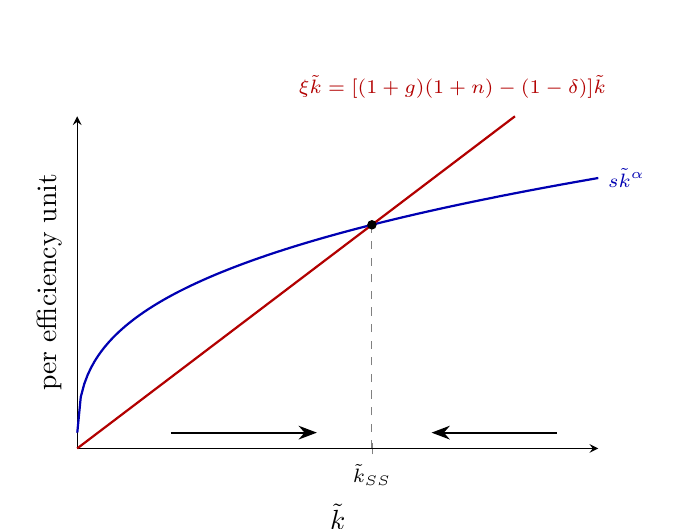
\begin{tikzpicture}
\begin{axis}[width=8.2cm,height=5.8cm,axis lines=left,xmin=0,xmax=5,ymin=0,ymax=0.42,clip=false,
  xlabel={$\tilde k$},ylabel={per efficiency unit},xtick={2.828},xticklabels={$\tilde k_{SS}$},ytick=\empty,
  every tick label/.append style={font=\scriptsize}]
\addplot[domain=0.001:5,samples=150,thick,blue!70!black]{0.2*x^(1/3)};
\addplot[domain=0:4.2,thick,red!70!black]{0.1*x};
\node[font=\scriptsize,blue!70!black,anchor=west] at (axis cs:5,0.342){$s\tilde k^{\alpha}$};
\node[font=\scriptsize,red!70!black,anchor=south] at (axis cs:3.6,0.43){$\xi\tilde k=[(1+g)(1+n)-(1-\delta)]\tilde k$};
\draw[dashed,gray](axis cs:2.828,0)--(axis cs:2.828,0.2828);
\addplot[only marks,mark=*,mark size=1.5pt]coordinates{(2.828,0.2828)};
\draw[-{Stealth},thick](axis cs:0.9,0.02)--(axis cs:2.3,0.02);
\draw[-{Stealth},thick](axis cs:4.6,0.02)--(axis cs:3.4,0.02);
\end{axis}
\end{tikzpicture}\\
{\footnotesize Figure 1. Steady state per efficiency unit. Left of $\tilde k_{SS}$ investment exceeds break-even
investment and $\tilde k$ rises; right of it, $\tilde k$ falls. (Drawn for $\alpha=1/3$, $s=0.2$, $\xi=0.1$.)}
\end{center}
\intuicao{Solow with technological progress is the no-progress model with one change of units: count
workers in efficiency units and the economy settles at a constant $\tilde k$; in per-worker units that same
point is a path growing at $g$.}
\refbib{Kurlat \S4.2, pp.~57--61 (law of motion, steady state, stability); \S4.5, pp.~69--72 (efficiency units,
balanced growth path).}
\rubrica{
\item Stationary variables defined and $\tilde y=\tilde k^{\alpha}$: 0.2 pt.
\item Ratio $\tilde k_{t+1}/\tilde k_t$ with $(1+g)(1+n)$ in the denominator: 0.3 pt.
\item $\tilde k_{SS}$: 0.2 pt. Diagram (axes, both curves named, $\tilde k_{SS}$ marked): 0.1 pt.
\item Growth rates of $y$ and $Y$ with the reason: 0.2 pt.
\item Dividing (2) by $A_tL_t$ instead of $A_{t+1}L_{t+1}$ (no $(1+g)(1+n)$): max.\ 0.5 pt. Working with $K/L$ as if stationary: max.\ 0.4 pt.
}
\end{sol}

\sub{2.b}{1 point} Show which saving rate maximises steady-state consumption per efficiency unit
of labour (the golden-rule rate, $s_{GR}$). Explain why the same $s_{GR}$ also maximises consumption
per worker at every date along the steady state, and how a faster rate of technological progress
$g$ changes $s_{GR}$ and $\tilde k_{GR}$. Give the economic intuition.
\resolespaco[7cm]
\begin{sol}
\begin{notacao}
\item As in 2.a. New: $\tilde c_{SS}(s)$, steady-state consumption per efficiency unit as a function
of the saving rate.
\item $f(\tilde k)\equiv\tilde k^{\alpha}$: output per efficiency unit, by \eqref{q2a:y}.
\item $s_{GR}\in(0,1)$, $\tilde k_{GR}>0$: golden-rule saving rate and capital per efficiency unit.
\item $c_t\equiv C_t/L_t$: consumption per worker. $A_0>0$: technology at date 0.
\end{notacao}
\passo{consumption in steady state}{Consumption is the part of output not saved:}
\begin{equation}
\tilde c_t=(1-s)\,\tilde y_t. \label{q2b:c}
\end{equation}
Substitute \eqref{q2a:yss} into \eqref{q2b:c}, carrying the exponent $\alpha$ of
$\tilde k_{SS}^{\alpha}$ through the substitution:
\begin{align}
\tilde c_{SS}(s) &= (1-s)\,\tilde k_{SS}^{\alpha}\nonumber\\
&= (1-s)\left[\left(\frac{s}{\xi}\right)^{\frac{1}{1-\alpha}}\right]^{\alpha}\nonumber\\
&= (1-s)\left(\frac{s}{\xi}\right)^{\frac{\alpha}{1-\alpha}}. \label{q2b:css}
\end{align}
\passo{first-order condition}{Take the log of \eqref{q2b:css}:}
\begin{equation}
\ln\tilde c_{SS}=\ln(1-s)+\frac{\alpha}{1-\alpha}\ln s-\frac{\alpha}{1-\alpha}\ln\xi. \label{q2b:log}
\end{equation}
Differentiate \eqref{q2b:log} with respect to $s$ and set it to zero:
\begin{equation}
\frac{d\ln\tilde c_{SS}}{ds}=-\frac{1}{1-s}+\frac{\alpha}{(1-\alpha)s}=0. \label{q2b:foc}
\end{equation}
Multiply \eqref{q2b:foc} by $(1-\alpha)s(1-s)>0$:
\begin{align*}
-(1-\alpha)s+\alpha(1-s) &= 0\\
\alpha(1-s) &= (1-\alpha)s\\
\alpha-\alpha s &= s-\alpha s\\
\alpha &= s.
\end{align*}
Hence
\begin{equation}
\boxed{s_{GR}=\alpha} \label{q2b:sgr}
\end{equation}
SOC: differentiate \eqref{q2b:foc} once more:
\[
\frac{d^2\ln\tilde c_{SS}}{ds^2}=-\frac{1}{(1-s)^2}-\frac{\alpha}{(1-\alpha)s^2}<0,
\]
so \eqref{q2b:sgr} is a maximum.
\passo{cross-check by $\tilde k$}{Substitute \eqref{q2a:y} into \eqref{q2b:c}, then use the
steady-state condition \eqref{q2a:break}, $s\tilde k^{\alpha}=\xi\tilde k$:}
\begin{align}
\tilde c &= (1-s)\big(\tilde k^{\alpha}\big)\nonumber\\
&= \tilde k^{\alpha}-s\tilde k^{\alpha}\nonumber\\
&= \tilde k^{\alpha}-\big(\xi\tilde k\big). \label{q2b:ck}
\end{align}
Maximise \eqref{q2b:ck} over $\tilde k$:
\begin{equation}
\boxed{f'(\tilde k_{GR})=\alpha\tilde k_{GR}^{\alpha-1}=\xi=(1+g)(1+n)-(1-\delta)} \label{q2b:mpk}
\end{equation}
The marginal product of capital equals break-even investment per unit of capital. Solve
\eqref{q2b:mpk} for $\tilde k_{GR}$:
\begin{equation}
\tilde k_{GR}^{1-\alpha}=\frac{\alpha}{\xi}. \label{q2b:kgr}
\end{equation}
Solve \eqref{q2a:break} for $s$ at $\tilde k_{GR}$ and use \eqref{q2b:kgr} in the third line:
\begin{align*}
s &= \frac{\xi\tilde k_{GR}}{\tilde k_{GR}^{\alpha}}\\
&= \xi\,\tilde k_{GR}^{1-\alpha}\\
&= \xi\cdot\frac{\alpha}{\xi}\\
&= \alpha\ \checkmark
\end{align*}
\passo{per worker, every date}{Invert \eqref{q2a:def} and use \eqref{q2:A}:}
\begin{align}
c_t &= \frac{C_t}{L_t}=A_t\,\tilde c_{SS}\nonumber\\
&= A_0(1+g)^t\,\tilde c_{SS}. \label{q2b:cpw}
\end{align}
Take logs of \eqref{q2b:cpw}:
\begin{equation}
\ln c_t=\ln A_0+t\ln(1+g)+\ln\tilde c_{SS}(s). \label{q2b:lncpw}
\end{equation}
$A_t$ does not depend on $s$, so the $s$ that maximises $\tilde c_{SS}$ raises the whole path
\eqref{q2b:lncpw} by the same amount at every $t$: the golden rule maximises consumption per worker
at \emph{every} date of the steady state.
\passo{effect of $g$}{$g$ does not appear in \eqref{q2b:sgr}: $s_{GR}=\alpha$ is
\textbf{unchanged}. Solving \eqref{q2b:kgr},}
\[
\tilde k_{GR}=\left(\frac{\alpha}{\xi}\right)^{\frac{1}{1-\alpha}},
\]
and by \eqref{q2a:xi}, $\partial\xi/\partial g=1+n>0$, so $\boxed{\tilde k_{GR}\downarrow}$. Faster
progress makes keeping $\tilde k$ constant more expensive (steeper break-even line), so the
consumption-maximising capital per efficiency unit is lower; but the \emph{share} of output to save
does not move, because with Cobb--Douglas the capital income $\alpha\tilde y$ always equals the
break-even investment $\xi\tilde k$ exactly at the golden rule.
\passo{knife-edge check}{$\alpha\to0$: capital is useless and $s_{GR}\to0$ in \eqref{q2b:sgr}.
Dropping the exponent (using $(s/\xi)^{1/(1-\alpha)}$ for $\tilde y$ in \eqref{q2b:css}) gives
$s=1/(2-\alpha)\to1/2$, which fails this test.}
\begin{center}
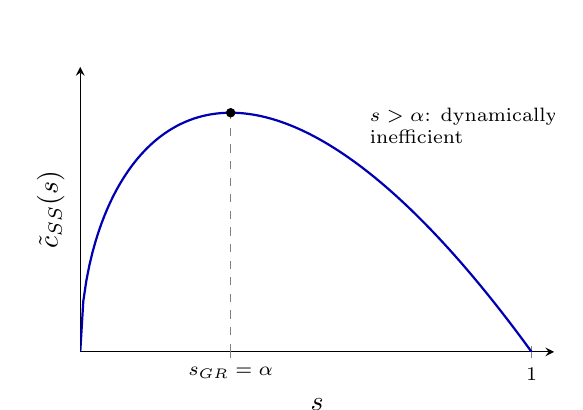
\begin{tikzpicture}
\begin{axis}[width=7.6cm,height=5.2cm,axis lines=left,xmin=0,xmax=1.05,ymin=0,ymax=1.45,
  xlabel={$s$},ylabel={$\tilde c_{SS}(s)$},xtick={0.3333,1},xticklabels={$s_{GR}=\alpha$,$1$},ytick=\empty,
  every tick label/.append style={font=\scriptsize}]
\addplot[domain=0:1,samples=150,thick,blue!70!black]{(1-x)*sqrt(x/0.1)};
\draw[dashed,gray](axis cs:0.3333,0)--(axis cs:0.3333,1.217);
\addplot[only marks,mark=*,mark size=1.5pt]coordinates{(0.3333,1.217)};
\node[font=\scriptsize,anchor=west,align=left] at (axis cs:0.62,1.15){$s>\alpha$: dynamically\\inefficient};
\end{axis}
\end{tikzpicture}\\
{\footnotesize Figure 2. Steady-state consumption per efficiency unit against $s$ (drawn for $\alpha=1/3$, $\xi=0.1$):
zero at $s=0$ (nothing to consume from) and at $s=1$ (nothing consumed), maximum at $s=\alpha$.}
\end{center}
\intuicao{Saving more raises $\tilde k$ and output, but each extra unit of capital also needs $\xi$ of
investment every period just to be kept per efficiency unit. Consumption is maximised when the last unit
of capital produces exactly what it costs to maintain: $f'(\tilde k)=\xi$. Above that point ($s>\alpha$) the
economy could consume more today and forever by saving less.}
\refbib{Kurlat \S4.3, pp.~61--63 (golden rule, $s_{gold}=\alpha$); \S4.5, pp.~69--72.}
\rubrica{
\item $\tilde c_{SS}(s)$ with exponent $\alpha/(1-\alpha)$: 0.3 pt.
\item FOC and $s_{GR}=\alpha$ (SOC or cross-check $f'=\xi$): 0.3 pt.
\item Per-worker consumption at every date maximised: 0.2 pt. Effect of $g$ on $s_{GR}$ and $\tilde k_{GR}$: 0.1 pt.
\item Intuition (marginal product equals break-even cost): 0.1 pt.
\item Exponent dropped in the substitution ($s=1/(2-\alpha)$): max.\ 0.4 pt. Maximising $\tilde k$ (answer $s=1$): max.\ 0.2 pt.
}
\gap{Prova 01, 2.b: the $\sigma$ (here $\alpha$) in the exponent of $c_{SS}$ was dropped.}
\end{sol}

\sub{2.c}{1 point} Consider now the competitive equilibrium of an economy that lasts only two
periods, $t=1,2$. There is an initial capital stock $K_1>0$, which belongs to the representative
firm and depreciates fully once used in period~1. The representative firm maximises profits in
perfectly competitive markets and has production function (1) in both periods, with
$A_2=(1+g)A_1$. The representative consumer owns the firm and receives its profits $\Pi_1$ and
$\Pi_2$. In each period the consumer has one unit of time, which it splits between work $L_t$ and
leisure $1-L_t$, and earns real labour income $w_tA_tL_t$ ($w_t$ is the real wage per efficiency
unit of labour). Income not consumed in period~1 is saved as an asset $a_1$ that pays the real
interest rate $r$; the only asset in this economy is the capital the firm uses in period~2, $K_2$,
which also depreciates fully once used. Intertemporal utility is
\[
U=\ln c_1+\gamma\ln(1-L_1)+\beta\left[\ln c_2+\gamma\ln(1-L_2)\right],\qquad \beta\in(0,1),\ \gamma>0.
\]
Derive and explain the intertemporal budget constraint of this consumer.
\resolespaco[6cm]
\begin{sol}
\begin{notacao}
\item $c_1$, $c_2>0$: consumption in periods 1 and 2. $L_t\in[0,1]$: hours worked; $1-L_t$: leisure
(time endowment normalised to 1).
\item $A_t>0$: technology, with $A_2=(1+g)A_1$. $w_t>0$: real wage per efficiency unit of labour, so
labour income is $w_tA_tL_t$.
\item $\Pi_1$, $\Pi_2$: the firm's profits, paid to the consumer who owns it.
\item $a_1$: asset carried from period 1 to period 2; of either sign for one consumer (in
equilibrium it is the capital $K_2>0$). $r>-1$: real interest rate between the periods.
\item $\beta\in(0,1)$: discount factor. $\gamma>0$: weight of leisure in utility.
\item $H>0$: full lifetime income, the present value of the time endowment plus profits (step 3).
\end{notacao}
\passo{period constraints}{In period 1, uses equal sources:}
\begin{equation}
\boxed{c_1+a_1=w_1A_1L_1+\Pi_1} \label{q2c:b1}
\end{equation}
Period 2 is the last: nothing is left for later, and nobody would lend to a consumer who cannot
repay after period 2. So the consumer spends the asset with its return plus period-2 income:
\begin{equation}
\boxed{c_2=(1+r)a_1+w_2A_2L_2+\Pi_2} \label{q2c:b2}
\end{equation}
Profits appear because the consumer owns the firm; with no initial financial wealth, they are its
only non-labour income besides the return on $a_1$.
\passo{eliminate $a_1$}{Solve \eqref{q2c:b2} for $a_1$:}
\begin{equation}
a_1=\frac{c_2-w_2A_2L_2-\Pi_2}{1+r}. \label{q2c:a1}
\end{equation}
Substitute \eqref{q2c:a1} into \eqref{q2c:b1}:
\[
c_1+\frac{c_2-w_2A_2L_2-\Pi_2}{1+r}=w_1A_1L_1+\Pi_1 .
\]
Move the period-2 income terms to the right side:
\begin{equation}
\boxed{c_1+\frac{c_2}{1+r}=w_1A_1L_1+\Pi_1+\frac{w_2A_2L_2+\Pi_2}{1+r}} \label{q2c:ibc}
\end{equation}
\passo{full-income form}{Value leisure at its opportunity cost, the wage. Add
$w_1A_1(1-L_1)+\frac{w_2A_2(1-L_2)}{1+r}$ to both sides of \eqref{q2c:ibc}; on the right,
$w_tA_tL_t+w_tA_t(1-L_t)=w_tA_t$:}
\begin{align}
&c_1+w_1A_1(1-L_1)+\frac{c_2+w_2A_2(1-L_2)}{1+r}\nonumber\\
&\qquad=\big[w_1A_1L_1+w_1A_1(1-L_1)\big]+\Pi_1+\frac{\big[w_2A_2L_2+w_2A_2(1-L_2)\big]+\Pi_2}{1+r}\nonumber\\
&\qquad=H, \label{q2c:full}
\end{align}
where
\begin{equation}
H\equiv w_1A_1+\Pi_1+\frac{w_2A_2+\Pi_2}{1+r}. \label{q2c:H}
\end{equation}
\passo{reading}{By \eqref{q2c:full}--\eqref{q2c:H}, the \textbf{present value} of lifetime
consumption (and of leisure, priced at the wage) equals the present value of lifetime income: the
value of the whole time endowment plus profits, with period-2 amounts discounted at $1+r$. $a_1$ may
be of either sign for one consumer; it disappears from the lifetime constraint \eqref{q2c:ibc}
because borrowing and lending only move resources across periods at the price $1/(1+r)$. The
constraint binds: $u'>0$, so unspent resources at the end are never optimal.}
\refbib{Kurlat \S6.2, pp.~105--112 (intertemporal budget constraint); \S7.2, pp.~131--137 (time endowment,
labour income); ch.~9, \S9.1 (households own the firms).}
\rubrica{
\item Two period constraints, with $\Pi_1,\Pi_2$ and the labour income of both periods: 0.4 pt.
\item Elimination of $a_1$ to the present-value constraint: 0.3 pt.
\item Explanation as a present-value statement (why $1+r$ discounts, why it binds): 0.3 pt.
\item Profits omitted: $-0.2$. ``Consumption adjusted by $r$'' without the present-value reading: max.\ 0.1 on the last line.
}
\gap{Prova 01, 2.c: firm profits omitted from the budget constraint; reading not stated in present value.}
\end{sol}

\sub{2.d}{1 point} Set up the problem of the consumer of item 2.c and derive the first-order
conditions for \emph{all} of its choice variables, including the equation describing the
intertemporal consumption decision and the consumption--leisure decision in each period. Then find
the equation that gives the optimal $c_1$ as a function only of parameters, prices and levels of
income and wealth, and interpret it economically.
\resolespaco[7cm]
\begin{sol}
\begin{notacao}
\item As in 2.c. New: $\lambda_1$, $\lambda_2>0$, the multipliers on \eqref{q2c:b1} and
\eqref{q2c:b2}: the marginal utility of one more unit of income in period $t$.
\end{notacao}
\passo{problem}{Choice variables: $c_1,c_2,L_1,L_2,a_1$; prices $w_1,w_2,r$ and profits
$\Pi_1,\Pi_2$ are taken as given. Maximise $U$ subject to \eqref{q2c:b1} and \eqref{q2c:b2}, with
one multiplier per period constraint:}
\begin{align}
\mathcal L={}&\ln c_1+\gamma\ln(1-L_1)+\beta\ln c_2+\beta\gamma\ln(1-L_2)\nonumber\\
&+\lambda_1\left[w_1A_1L_1+\Pi_1-c_1-a_1\right]+\lambda_2\left[(1+r)a_1+w_2A_2L_2+\Pi_2-c_2\right]. \label{q2d:lag}
\end{align}
\passo{FOCs}{Differentiate \eqref{q2d:lag} with respect to each choice variable and set the
derivative to zero:}
\begin{align}
c_1:&\quad \frac{1}{c_1}=\lambda_1, \label{q2d:c1}\\
c_2:&\quad \frac{\beta}{c_2}=\lambda_2, \label{q2d:c2}\\
L_1:&\quad \frac{\gamma}{1-L_1}=\lambda_1w_1A_1, \label{q2d:L1}\\
L_2:&\quad \frac{\beta\gamma}{1-L_2}=\lambda_2w_2A_2, \label{q2d:L2}\\
a_1:&\quad \lambda_1=(1+r)\lambda_2. \label{q2d:a1}
\end{align}
Log utility makes every solution interior: as $L_t\to1$ the marginal utility of leisure goes to
infinity, and as $c_t\to0$ that of consumption does.
\passo{Euler (intertemporal)}{Substitute \eqref{q2d:c1} and \eqref{q2d:c2} into \eqref{q2d:a1}:}
\begin{align*}
\left(\frac{1}{c_1}\right) &= (1+r)\left(\frac{\beta}{c_2}\right)\\
\frac{1}{c_1} &= \beta(1+r)\frac{1}{c_2}.
\end{align*}
Multiply by $c_1c_2$:
\begin{equation}
\boxed{c_2=\beta(1+r)\,c_1} \label{q2d:euler}
\end{equation}
The marginal rate of substitution between $c_1$ and $c_2$ equals the relative price $1+r$.
\passo{consumption--leisure (intratemporal)}{Divide \eqref{q2d:L1} by \eqref{q2d:c1}, and
\eqref{q2d:L2} by \eqref{q2d:c2}; the multipliers cancel:}
\begin{align*}
\frac{\gamma/(1-L_1)}{1/c_1} &= \frac{\lambda_1w_1A_1}{\lambda_1},\\
\frac{\beta\gamma/(1-L_2)}{\beta/c_2} &= \frac{\lambda_2w_2A_2}{\lambda_2}.
\end{align*}
\begin{equation}
\boxed{\frac{\gamma c_1}{1-L_1}=w_1A_1} \label{q2d:intra1}
\end{equation}
\begin{equation}
\boxed{\frac{\gamma c_2}{1-L_2}=w_2A_2} \label{q2d:intra2}
\end{equation}
In each period the MRS between leisure and consumption equals the real wage (the price of an hour
of leisure).
\passo{solve for $c_1$}{Express each term on the left of the full-income constraint
\eqref{q2c:full} in terms of $c_1$. From \eqref{q2d:euler}, \eqref{q2d:intra1}, and
\eqref{q2d:intra2} followed by \eqref{q2d:euler}:}
\begin{align}
\frac{c_2}{1+r} &= \frac{\big[\beta(1+r)c_1\big]}{1+r}\nonumber\\
&= \beta c_1, \label{q2d:t1}\\
w_1A_1(1-L_1) &= \gamma c_1, \label{q2d:t2}\\
\frac{w_2A_2(1-L_2)}{1+r} &= \frac{\gamma c_2}{1+r}\nonumber\\
&= \frac{\gamma\big[\beta(1+r)c_1\big]}{1+r}\nonumber\\
&= \beta\gamma c_1. \label{q2d:t3}
\end{align}
Split the fraction in \eqref{q2c:full} and substitute \eqref{q2d:t1}--\eqref{q2d:t3}:
\begin{align*}
c_1+w_1A_1(1-L_1)+\frac{c_2}{1+r}+\frac{w_2A_2(1-L_2)}{1+r} &= H\\
c_1+(\gamma c_1)+(\beta c_1)+(\beta\gamma c_1) &= H\\
c_1(1+\gamma+\beta+\beta\gamma) &= H\\
c_1(1+\beta)(1+\gamma) &= H.
\end{align*}
Divide by $(1+\beta)(1+\gamma)$ and write $H$ out with \eqref{q2c:H}:
\begin{align}
c_1 &= \frac{H}{(1+\beta)(1+\gamma)}\nonumber\\
&= \boxed{\frac{1}{(1+\beta)(1+\gamma)}\left[w_1A_1+\Pi_1+\frac{w_2A_2+\Pi_2}{1+r}\right]} \label{q2d:c1sol}
\end{align}
Then \eqref{q2d:euler}, \eqref{q2d:intra1}--\eqref{q2d:intra2} and \eqref{q2c:b1} give the other
choices:
\begin{align*}
c_2 &= \beta(1+r)\,c_1,\\
1-L_t &= \frac{\gamma c_t}{w_tA_t},\quad t=1,2,\\
a_1 &= w_1A_1L_1+\Pi_1-c_1.
\end{align*}
\passo{interpretation}{By \eqref{q2d:t1}--\eqref{q2d:c1sol}, with log utility the consumer spends fixed shares of full lifetime wealth $H$:
$\frac{1}{(1+\beta)(1+\gamma)}$ on $c_1$, $\frac{\gamma}{(1+\beta)(1+\gamma)}$ on leisure in period 1,
$\frac{\beta}{(1+\beta)(1+\gamma)}$ and $\frac{\beta\gamma}{(1+\beta)(1+\gamma)}$ on period~2.
$c_1$ depends on \emph{lifetime} resources, not on period-1 income alone (permanent income).
$\beta\uparrow\Rightarrow c_1\downarrow$ (patience moves spending to period 2); $\gamma\uparrow\Rightarrow
c_1\downarrow$ for given $H$ (more of full wealth is taken as leisure). Given $H$, $r$ does not enter: for
the shares, the income and substitution effects of $r$ cancel with log utility; $r$ moves $c_1$ only
through the present value of period-2 income in $H$ (a higher $r$ lowers it, so $c_1$ falls).}
\intuicao{Contrast with Prova 01: there work had no utility cost, so $L_1=1$ was a corner and saying so
was the FOC. Here leisure is valued, so hours are an interior choice and the wage is the price of leisure.}
\refbib{Kurlat \S6.2, pp.~105--115 (Euler equation, log closed forms); \S7.2, pp.~131--137 (consumption--leisure);
ch.~9, \S9.1, eq.~(9.1.7)--(9.1.8).}
\rubrica{
\item Problem stated with all five choice variables: 0.1 pt.
\item FOCs for $c_1,c_2$ and the Euler equation: 0.3 pt. FOCs for $L_1$ and $L_2$ (intratemporal conditions): 0.2 pt (0.1 each).
\item FOC for $a_1$ (or the substitution that eliminates it): 0.1 pt.
\item $c_1$ in closed form: 0.2 pt. Interpretation ($H$, $\beta$, $\gamma$, role of $r$): 0.1 pt.
\item No FOC for hours: max.\ 0.6 pt. Substitution route instead of Lagrangian: full credit.
}
\gap{Prova 01, 2.d: FOC for $L_1$ missing (``todas as variáveis de sua escolha'').}
\end{sol}

\sub{2.e}{1 point} Calculate the saving rate of this representative consumer (the share of saving
in the consumer's period-1 income), recalling that markets are perfectly competitive. Find the hours
worked in each period. Then find an expression for $\hat k_2\equiv K_2/A_2$ as a function only of
$\hat k_1\equiv K_1/A_1$ and of parameters. Treating this expression as a law of motion that applies
period after period, draw it with $\hat k_1$ on the horizontal axis and $\hat k_2$ on the vertical
axis, and show graphically the steady state of this economy. Is it stable? Justify.
\resolespaco[8cm]
\begin{sol}
\begin{notacao}
\item As in 2.c--2.d. New: $Y_1$, $Y_2>0$, output in each period by \eqref{q2:Y}; $K_2>0$, the
capital built from period-1 saving.
\item $s^\ast\in(0,1)$: the consumer's saving rate. $\hat k_t\equiv K_t/A_t>0$: capital per unit of
technology.
\item $\phi(\hat k)$: the law of motion $\hat k_{t+1}=\phi(\hat k_t)$. $\hat k_{SS}$: its fixed point.
$\hat k_{GR}$ (Figure 3): the fixed point of the same map with $s=s_{GR}$.
\end{notacao}
\passo{firm, period 1}{The firm owns $K_1$ and hires labour:}
\begin{equation}
\max_{L_1}\ K_1^{\alpha}(A_1L_1)^{1-\alpha}-w_1A_1L_1. \label{q2e:firm1}
\end{equation}
The FOC of \eqref{q2e:firm1}, with $Y_1$ from \eqref{q2:Y}:
\begin{equation}
(1-\alpha)\frac{Y_1}{L_1}=w_1A_1. \label{q2e:foc1}
\end{equation}
Multiply \eqref{q2e:foc1} by $L_1$ to get the wage bill:
\begin{equation}
w_1A_1L_1=(1-\alpha)Y_1. \label{q2e:wb1}
\end{equation}
Profit is output minus the wage bill \eqref{q2e:wb1}:
\begin{align}
\Pi_1 &= Y_1-w_1A_1L_1\nonumber\\
&= Y_1-(1-\alpha)Y_1\nonumber\\
&= \boxed{\alpha Y_1}, \label{q2e:pi1}
\end{align}
the return on the capital the firm owns, paid to its owner.
\passo{firm, period 2}{The firm borrows $K_2$ from the consumer and repays $(1+r)K_2$ (the capital
is used up):}
\begin{equation}
\max_{K_2,L_2}\ K_2^{\alpha}(A_2L_2)^{1-\alpha}-w_2A_2L_2-(1+r)K_2. \label{q2e:firm2}
\end{equation}
The FOCs of \eqref{q2e:firm2}:
\begin{align}
\alpha\frac{Y_2}{K_2} &= 1+r, \label{q2e:r}\\
(1-\alpha)\frac{Y_2}{L_2} &= w_2A_2. \label{q2e:w2}
\end{align}
Multiply \eqref{q2e:r} by $K_2$ and \eqref{q2e:w2} by $L_2$ and subtract both payments from output.
With constant returns:
\begin{align}
\Pi_2 &= Y_2-w_2A_2L_2-(1+r)K_2\nonumber\\
&= Y_2-(1-\alpha)Y_2-\alpha Y_2\nonumber\\
&= \boxed{0}. \label{q2e:pi2}
\end{align}
\passo{market clearing}{The only asset is the capital of period 2, so the asset market clears when}
\begin{equation}
\boxed{a_1=K_2} \label{q2e:mc}
\end{equation}
The goods markets clear when
\begin{align}
c_1+K_2 &= Y_1, \label{q2e:g1}\\
c_2 &= Y_2. \label{q2e:g2}
\end{align}
Labour: $L_t$ supplied $=$ $L_t$ demanded. Check: by \eqref{q2e:r}, \eqref{q2e:w2} and
\eqref{q2e:pi2}, period-2 income in \eqref{q2c:b2} is
\[
(1+r)K_2+w_2A_2L_2+\Pi_2=\alpha Y_2+(1-\alpha)Y_2+0=Y_2 .
\]
\passo{saving rate}{Substitute \eqref{q2e:g2} and \eqref{q2e:r} into the Euler equation
\eqref{q2d:euler}, then multiply by $K_2/Y_2$:}
\begin{align}
(Y_2) &= \beta\left(\frac{\alpha Y_2}{K_2}\right)c_1\nonumber\\
K_2 &= \alpha\beta\,c_1. \label{q2e:K2c1}
\end{align}
Substitute \eqref{q2e:K2c1} into the period-1 goods market \eqref{q2e:g1}:
\begin{align}
c_1+(\alpha\beta c_1) &= Y_1\nonumber\\
c_1 &= \frac{Y_1}{1+\alpha\beta}. \label{q2e:c1}
\end{align}
Substitute \eqref{q2e:c1} into \eqref{q2e:K2c1} and use \eqref{q2e:mc}:
\begin{align}
K_2 &= \alpha\beta\left(\frac{Y_1}{1+\alpha\beta}\right)\nonumber\\
a_1=K_2 &= \frac{\alpha\beta}{1+\alpha\beta}\,Y_1. \label{q2e:a1}
\end{align}
Period-1 income, by \eqref{q2e:wb1} and \eqref{q2e:pi1}:
\begin{align}
w_1A_1L_1+\Pi_1 &= (1-\alpha)Y_1+\alpha Y_1\nonumber\\
&= Y_1. \label{q2e:inc1}
\end{align}
Divide \eqref{q2e:a1} by \eqref{q2e:inc1}:
\begin{align}
s^\ast &= \frac{a_1}{w_1A_1L_1+\Pi_1}\nonumber\\
&= \frac{\left(\frac{\alpha\beta}{1+\alpha\beta}\,Y_1\right)}{(Y_1)}\nonumber\\
&= \boxed{\frac{\alpha\beta}{1+\alpha\beta}}\quad\text{(constant: no }K_1,A_1,g,\gamma\text{)}. \label{q2e:s}
\end{align}
\passo{hours}{Period 2: substitute \eqref{q2e:g2} for $c_2$ and \eqref{q2e:w2} for $w_2A_2$ into
\eqref{q2d:intra2}:}
\begin{align}
\frac{\gamma(Y_2)}{1-L_2} &= \left(\frac{(1-\alpha)Y_2}{L_2}\right)\nonumber\\
\gamma L_2 &= (1-\alpha)(1-L_2)\nonumber\\
L_2(1-\alpha+\gamma) &= 1-\alpha\nonumber\\
L_2 &= \boxed{\frac{1-\alpha}{1-\alpha+\gamma}}. \label{q2e:L2}
\end{align}
Period 1: substitute \eqref{q2e:c1} for $c_1$ and \eqref{q2e:foc1} for $w_1A_1$ into
\eqref{q2d:intra1}:
\begin{align}
\frac{\gamma\left(\frac{Y_1}{1+\alpha\beta}\right)}{1-L_1} &= \left(\frac{(1-\alpha)Y_1}{L_1}\right)\nonumber\\
\frac{\gamma Y_1}{(1+\alpha\beta)(1-L_1)} &= \frac{(1-\alpha)Y_1}{L_1}\nonumber\\
\gamma L_1 &= (1-\alpha)(1+\alpha\beta)(1-L_1)\nonumber\\
L_1\big[(1-\alpha)(1+\alpha\beta)+\gamma\big] &= (1-\alpha)(1+\alpha\beta)\nonumber\\
L_1 &= \boxed{\frac{(1-\alpha)(1+\alpha\beta)}{(1-\alpha)(1+\alpha\beta)+\gamma}}. \label{q2e:L1}
\end{align}
Neither \eqref{q2e:L2} nor \eqref{q2e:L1} depends on $K_1$ or $A_t$: with log utility the income and
substitution effects of a higher wage cancel. $L_1>L_2$: in period 1 consumption is only the share
$1/(1+\alpha\beta)$ of output, so a unit of income is worth more at the margin (part of it is saved)
and the consumer works more.
\passo{law of motion}{By \eqref{q2e:a1}, \eqref{q2e:s} and \eqref{q2:Y}:}
\begin{align}
K_2 &= s^\ast Y_1\nonumber\\
&= s^\ast K_1^{\alpha}(A_1L_1)^{1-\alpha}. \label{q2e:K2}
\end{align}
Divide \eqref{q2e:K2} by $A_2=(1+g)A_1$ and use $K_1=\hat k_1A_1$:
\begin{align}
\hat k_2 &= \frac{s^\ast(\hat k_1A_1)^{\alpha}(A_1L_1)^{1-\alpha}}{(1+g)A_1}\nonumber\\
&= \frac{s^\ast A_1\,\hat k_1^{\alpha}L_1^{1-\alpha}}{(1+g)A_1}\nonumber\\
&= \boxed{\frac{s^\ast L_1^{1-\alpha}}{1+g}\,\hat k_1^{\alpha}}\equiv\phi(\hat k_1). \label{q2e:phi}
\end{align}
\passo{steady state and stability}{From \eqref{q2e:phi}: $\phi(0)=0$, $\phi'>0$, $\phi''<0$,
$\phi'\to\infty$ as $\hat k\to0$ and $\phi'\to0$ as $\hat k\to\infty$. The curve starts above the
45-degree line and ends below it, so it crosses it exactly once at a positive point. Set
$\hat k=\phi(\hat k)$ in \eqref{q2e:phi}:}
\begin{align*}
\hat k &= \frac{s^\ast L_1^{1-\alpha}}{1+g}\,\hat k^{\alpha}\\
\hat k^{1-\alpha} &= \frac{s^\ast L_1^{1-\alpha}}{1+g}.
\end{align*}
Raise both sides to the power $1/(1-\alpha)$:
\begin{equation}
\boxed{\hat k_{SS}=\left(\frac{s^\ast L_1^{1-\alpha}}{1+g}\right)^{\frac{1}{1-\alpha}}} \label{q2e:kss}
\end{equation}
Differentiate \eqref{q2e:phi}:
\begin{align*}
\phi'(\hat k) &= \alpha\,\frac{s^\ast L_1^{1-\alpha}}{1+g}\,\hat k^{\alpha-1}\\
&= \alpha\,\frac{\phi(\hat k)}{\hat k}.
\end{align*}
At the fixed point $\phi(\hat k_{SS})=\hat k_{SS}$, so
\begin{align*}
\phi'(\hat k_{SS}) &= \alpha\,\frac{\phi(\hat k_{SS})}{\hat k_{SS}}\\
&= \alpha\,\frac{(\hat k_{SS})}{\hat k_{SS}}\\
&= \alpha<1\ \Rightarrow\ \text{stable}.
\end{align*}
From any $\hat k_1<\hat k_{SS}$ the staircase between $\phi$ and the 45-degree line climbs
monotonically to $\hat k_{SS}$ (Figure 3).
\begin{center}
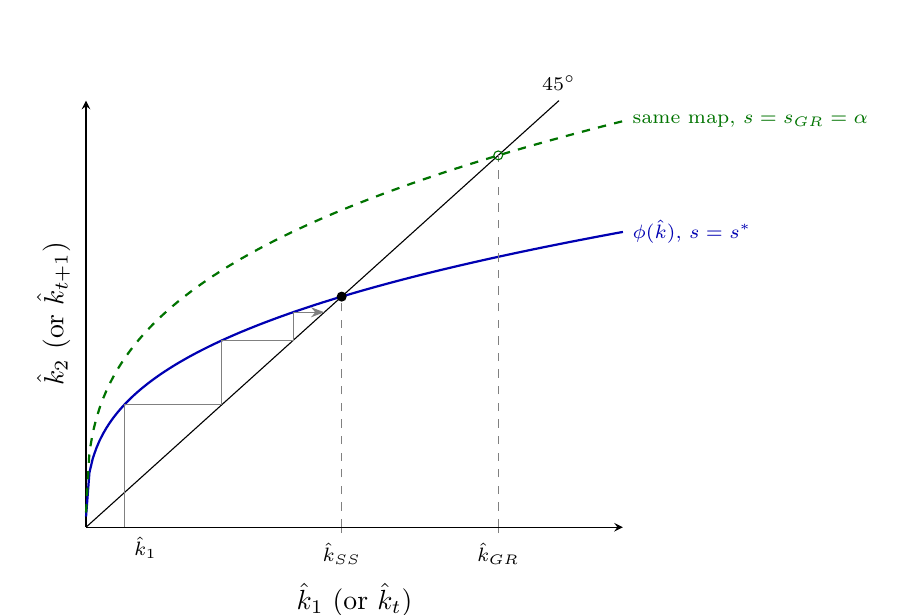
\begin{tikzpicture}
\begin{axis}[width=8.4cm,height=7cm,axis lines=left,xmin=0,xmax=2.1,ymin=0,ymax=1.85,clip=false,
  xlabel={$\hat k_1$ (or $\hat k_t$)},ylabel={$\hat k_2$ (or $\hat k_{t+1}$)},xtick={1,1.6124},
  xticklabels={$\hat k_{SS}$,$\hat k_{GR}$},ytick=\empty,every tick label/.append style={font=\scriptsize}]
\addplot[domain=0:1.85,thin,black]{x};
\addplot[domain=0.0001:2.1,samples=160,thick,blue!70!black]{x^(1/3)};
\addplot[domain=0.0001:2.1,samples=160,thick,dashed,green!45!black]{1.375*x^(1/3)};
\node[font=\scriptsize,anchor=south] at (axis cs:1.85,1.85){$45^\circ$};
\node[font=\scriptsize,blue!70!black,anchor=west] at (axis cs:2.1,1.281){$\phi(\hat k)$, $s=s^\ast$};
\node[font=\scriptsize,green!45!black,anchor=west] at (axis cs:2.1,1.761){same map, $s=s_{GR}=\alpha$};
\draw[gray,-{Stealth}](axis cs:0.15,0)--(axis cs:0.15,0.5313)--(axis cs:0.5313,0.5313)--(axis cs:0.5313,0.8099)
  --(axis cs:0.8099,0.8099)--(axis cs:0.8099,0.9321)--(axis cs:0.9321,0.9321);
\addplot[only marks,mark=*,mark size=1.6pt]coordinates{(1,1)};
\addplot[only marks,mark=o,mark size=1.6pt,green!45!black]coordinates{(1.6124,1.6124)};
\draw[dashed,gray](axis cs:1,0)--(axis cs:1,1);
\draw[dashed,gray](axis cs:1.6124,0)--(axis cs:1.6124,1.6124);
\node[font=\scriptsize,anchor=north west] at (axis cs:0.15,0){$\hat k_1$};
\end{axis}
\end{tikzpicture}\\
{\footnotesize Figure 3. The equilibrium law of motion (solid) crosses the 45-degree line once; the staircase
from a low $\hat k_1$ converges to $\hat k_{SS}$. Dashed: the same map with $s=\alpha$, whose fixed point is the
golden rule (used in 2.f). Drawn for $\alpha=1/3$, $\beta=0.96$, units chosen so that $\hat k_{SS}=1$.}
\end{center}
\intuicao{Patience and the productivity of capital set the saving rate; diminishing returns ($\alpha<1$) make
each extra unit of capital produce less, so saving a fixed share of a concave output cannot sustain unbounded
growth of $\hat k$.}
\refbib{Kurlat ch.~9, \S9.1 (firm FOCs, market clearing, $r=r^K-\delta$ with $\delta=1$); \S4.4, pp.~63--69
(factor shares, zero profit under constant returns); \S4.2, pp.~59--61 (stability).}
\rubrica{
\item Firm FOCs, $\Pi_1=\alpha Y_1$, $\Pi_2=0$, $1+r=\alpha Y_2/K_2$: 0.2 pt.
\item Market clearing $a_1=K_2$ (and goods): 0.1 pt. Saving rate $\alpha\beta/(1+\alpha\beta)$ derived: 0.2 pt.
\item Hours $L_1$, $L_2$: 0.1 pt. Map $\hat k_2(\hat k_1)$: 0.2 pt.
\item Diagram: axes, 45-degree line, concave map from the origin, $\hat k_{SS}$ at the crossing, stability argued: 0.2 pt.
\item Saving rate quoted from Solow's $s$ or left as a function of prices: 0 for that line. No market clearing ($K_2\neq a_1$): max.\ 0.5 pt. A map that does not cross the 45-degree line: 0 for the diagram.
}
\gap{Prova 01, 2.e: saving rate not derived; no market clearing $K_2=a_1$; diagram without a valid steady state.}
\end{sol}

\sub{2.f}{0.5 point} Discuss intuitively the relation between the model of items 2.c--2.e and the
Solow model of items 2.a--2.b. In particular, compare the saving rate found in 2.e with $s_{GR}$ and
explain the difference.
\resolespaco[5cm]
\begin{sol}
\begin{notacao}
\item As in 2.a--2.e. New: $\tilde k_t\equiv\hat k_t/L_1=K_t/(A_tL_1)>0$, capital per efficiency unit
of \emph{hours} (in 2.a, per efficiency unit of workers).
\end{notacao}
\passo{same law of motion}{Write \eqref{q2e:phi}, applied period after period, in terms of
$\tilde k_t=\hat k_t/L_1$:}
\begin{align}
L_1\tilde k_{t+1} &= \frac{s^\ast L_1^{1-\alpha}}{1+g}\,(L_1\tilde k_t)^{\alpha}\nonumber\\
&= \frac{s^\ast L_1}{1+g}\,\tilde k_t^{\alpha}\nonumber\\
(1+g)\tilde k_{t+1} &= s^\ast\tilde k_t^{\alpha}. \label{q2f:lom}
\end{align}
Set $\boxed{\delta=1}$ (capital used up in one period) and $\boxed{n=0}$ (one consumer) in the
Solow law of motion \eqref{q2a:lom}, which is equation \eqref{q2:K} divided as in 2.a:
\begin{align}
\tilde k_{t+1} &= \frac{(1-1)\tilde k_t+s\tilde k_t^{\alpha}}{(1+g)(1+0)}\nonumber\\
&= \frac{s\tilde k_t^{\alpha}}{1+g}\nonumber\\
(1+g)\tilde k_{t+1} &= s\,\tilde k_t^{\alpha}. \label{q2f:solow}
\end{align}
\eqref{q2f:lom} is \eqref{q2f:solow} with $s=s^\ast$. Indeed, by \eqref{q2e:kss},
\begin{align*}
\hat k_{SS} &= \left(\frac{s^\ast L_1^{1-\alpha}}{1+g}\right)^{\frac{1}{1-\alpha}}\\
&= L_1\left(\frac{s^\ast}{1+g}\right)^{\frac{1}{1-\alpha}}\\
&= L_1\left(\frac{s^\ast}{(1+g)(1+0)-(1-1)}\right)^{\frac{1}{1-\alpha}},
\end{align*}
which is 2.a's $\tilde k_{SS}$ \eqref{q2a:kss} times the hours worked.
\passo{what is new}{Solow \emph{assumes} $s$ and the labour input. Here both are \emph{chosen}:
$s^\ast=\alpha\beta/(1+\alpha\beta)$ in \eqref{q2e:s} comes from patience $\beta$ and the return to
capital $\alpha$, and log utility makes it constant (independent of $K$, $A$, $g$) --- a
microfoundation for Solow's constant saving rate. Hours $L_1$ in \eqref{q2e:L1} depend on the taste
for leisure $\gamma$ and on $\beta$.}
\passo{against the golden rule}{Compare \eqref{q2e:s} with $s_{GR}=\alpha$ from \eqref{q2b:sgr}:}
\begin{align*}
s^\ast<\alpha &\iff \frac{\alpha\beta}{1+\alpha\beta}<\alpha\\
&\iff \frac{\beta}{1+\alpha\beta}<1\\
&\iff \beta<1+\alpha\beta\\
&\iff \beta(1-\alpha)<1,
\end{align*}
always true, since $\beta<1$ and $1-\alpha<1$. So $\boxed{s^\ast<\alpha}$ and $\hat k_{SS}<\hat k_{GR}$
(Figure 3): the competitive economy accumulates \emph{less} than the golden rule. Even as
$\beta\to1$, $s^\ast\to\alpha/(1+\alpha)<\alpha$: here saving finances one period of consumption
only, since the horizon ends.
\passo{why this is not a failure}{The golden rule maximises steady-state consumption and ignores that
consumption earlier is worth more to an impatient consumer ($\beta<1$) and that reaching more capital costs
consumption on the way. Markets here are complete and competitive, with no externalities: by the first welfare
theorem the equilibrium is Pareto efficient, and it is below the golden rule, i.e.\ dynamically efficient. The
golden rule is a property of steady states, not a welfare criterion.}
\refbib{Kurlat \S4.3, pp.~61--63; ch.~9, \S9.2 (first welfare theorem) and \S9.3 (comparison with the golden rule).}
\rubrica{
\item Same law of motion with $\delta=1$, $n=0$: 0.1 pt.
\item Saving (and hours) chosen, not assumed, and from which primitives: 0.2 pt.
\item $s^\ast<\alpha$ shown, with the reason (impatience; golden rule not a welfare criterion): 0.2 pt.
\item ``It is Solow with $\delta=1$ and $n=0$'' and nothing else: max.\ 0.1 pt.
}
\gap{Prova 01, 2.f: the endogenous saving rate and its comparison with $s_{GR}$ were missing.}
\end{sol}

% =============================================================================
\questao{3}{3}{Consider the simplified New Keynesian model of Benigno (2015), based on the aggregate
demand and supply equations below (barred variables are long-run values, when all firms reset their
prices; the others are short-run values):
\begin{align}
y &= \bar y+(g-\bar g)-\sigma\left[i-(\bar p-p)\right]-\sigma\ln\beta, \tag{AD}\label{q3:AD}\\
p-p^e &= \kappa\,(y-y_n), \tag{AS}\label{q3:AS}
\end{align}
where $p^e$ is the price set by the firms that cannot reset prices and $y_n$ is short-run natural output,
\begin{equation}
y_n=\frac{1+\eta}{\sigma^{-1}+\eta}\,a+\frac{\sigma^{-1}}{\sigma^{-1}+\eta}\,g-\frac{1}{\sigma^{-1}+\eta}\,\mu , \tag{YN}\label{q3:YN}
\end{equation}
$\mu$ being the mark-up; $\bar y$ is given by the same expression evaluated at the long-run values
$\bar a$, $\bar g$, $\bar\mu$; and $y_e=\frac{1+\eta}{\sigma^{-1}+\eta}a+\frac{\sigma^{-1}}{\sigma^{-1}+\eta}g$ is the
efficient level of output. All variables are log deviations from an efficient steady state. Initially
$a=\bar a=g=\bar g=\mu=\bar\mu=0$, $\bar p=p^e$, and the central bank sets $i=\rho\equiv-\ln\beta$, so that
$y=y_n=y_e=\bar y$ and $p=p^e$.}

\sub{3.a}{1 point} News arrives that productivity will be permanently higher in the long run: $\bar a$
rises by $d\bar a>0$, while current productivity $a$ does not change. With $i$ unchanged, represent
graphically, explaining economically why, the initial equilibrium and the shift that defines the new
equilibrium. Compute $dy$ and $dp$. Indicate the gap $y-y_n$ and the gap $y-y_e$ and use both in your
explanation. Is this boom good for welfare today? Justify.
\resolespaco[7cm]
\begin{sol}
\begin{notacao}
\item $y$, $p$: output and price level today; $\bar y$, $\bar p$: their long-run values, when all
firms have reset prices. All are log deviations from the efficient steady state.
\item $p^e$: the price preset by the firms that cannot reset this period.
\item $i$: nominal interest rate, the central bank's instrument. $\beta\in(0,1)$: discount factor;
$\rho\equiv-\ln\beta>0$: the initial (neutral) rate.
\item $a$, $\bar a$: productivity today and in the long run. $g$, $\bar g$: government spending.
$\mu$, $\bar\mu$: the firms' mark-up. All start at 0.
\item $\sigma>0$: intertemporal elasticity of substitution. $\eta>0$: inverse Frisch elasticity of
labour supply. $\kappa>0$: slope of AS.
\item $y_n$: natural output (flexible prices, with the mark-up). $y_e$: efficient output (no mark-up).
\item $\Gamma\equiv\frac{1+\eta}{\sigma^{-1}+\eta}>0$: response of $y_n$, $y_e$ and $\bar y$ to
productivity.
\end{notacao}
\passo{0, the remaining statement equations}{With $\Gamma$ as defined above, the statement gives
long-run output (the expression \eqref{q3:YN} at long-run values) and efficient output:}
\begin{align}
\bar y &= \Gamma\,\bar a+\frac{\sigma^{-1}}{\sigma^{-1}+\eta}\,\bar g-\frac{1}{\sigma^{-1}+\eta}\,\bar\mu, \label{q3:ybar}\\
y_e &= \Gamma\,a+\frac{\sigma^{-1}}{\sigma^{-1}+\eta}\,g. \label{q3:ye}
\end{align}
Substitute $\rho=-\ln\beta$ into \eqref{q3:AD}, then use the initial values $g=\bar g=0$ and
$\bar p=p^e$:
\begin{align}
y &= \bar y+(g-\bar g)-\sigma\left[i-(\bar p-p)\right]-\sigma(-\rho)\nonumber\\
&= \bar y+(g-\bar g)-\sigma(i-\rho)-\sigma(p-\bar p)\nonumber\\
&= \bar y+(0-0)-\sigma(i-\rho)-\sigma\big(p-(p^e)\big)\nonumber\\
&= \bar y-\sigma(i-\rho)-\sigma(p-p^e). \label{q3:ADr}
\end{align}
\passo{which bar moves which curve}{Differentiate \eqref{q3:ybar} with only $\bar a$ moving:}
\begin{equation}
d\bar y=\Gamma\,d\bar a>0. \label{q3a:dybar}
\end{equation}
$\bar y$ is in AD \eqref{q3:ADr}, so \boxed{\text{AD shifts right}} by $\Gamma d\bar a$ at every
$p$ (up by $\Gamma d\bar a/\sigma$). $y_n$ in \eqref{q3:YN} and $y_e$ in \eqref{q3:ye} depend on the
\emph{current} $a$, $g$, $\mu$, none of which moved: \boxed{\text{AS does not move}} (it still passes
through $(y_n,p^e)$), and $y_e=y_n=0$ still.
\passo{why AD moves (Euler)}{Long-run consumption $\bar c=\bar y$ rises: households expect higher permanent
income and, to smooth consumption, want to consume more \emph{today} at the same real rate
$i-(\bar p-p)$. Current demand for goods rises at every price level.}
\passo{new equilibrium}{With $i=\rho$, \eqref{q3:ADr} and \eqref{q3a:dybar} give AD; with $y_n=0$,
\eqref{q3:AS} gives AS:}
\begin{align}
y &= (\Gamma\,d\bar a)-\sigma(\rho-\rho)-\sigma(p-p^e)\nonumber\\
&= \Gamma\,d\bar a-\sigma(p-p^e), \label{q3a:AD}\\
p-p^e &= \kappa\,(y-0)\nonumber\\
&= \kappa\,y. \label{q3a:AS}
\end{align}
Substitute \eqref{q3a:AS} into \eqref{q3a:AD}:
\begin{align*}
y &= \Gamma\,d\bar a-\sigma(\kappa\,y)\\
y(1+\sigma\kappa) &= \Gamma\,d\bar a.
\end{align*}
Divide by $1+\sigma\kappa$ (the initial $y$ is 0, so $y=dy$):
\begin{equation}
\boxed{dy=\frac{\Gamma\,d\bar a}{1+\sigma\kappa}>0} \label{q3a:dy}
\end{equation}
Substitute \eqref{q3a:dy} into \eqref{q3a:AS}:
\begin{align}
dp &= \kappa\,dy\nonumber\\
&= \kappa\left(\frac{\Gamma\,d\bar a}{1+\sigma\kappa}\right)\nonumber\\
&= \boxed{\frac{\kappa\,\Gamma\,d\bar a}{1+\sigma\kappa}>0}. \label{q3a:dp}
\end{align}
\passo{the two gaps}{Since $y_n=y_e=0$, both gaps equal \eqref{q3a:dy}. $y-y_n=dy>0$: output above
natural, which is why prices rise in \eqref{q3a:dp} (AS: flexible-price firms face higher real
marginal cost, because households must be paid a higher real wage to work more). $y-y_e=dy>0$:
output above the efficient level as well.
Chain: $\bar a\uparrow\to\bar y\uparrow\to c\uparrow$ (Euler) $\to$ AD right $\to y>y_n\to$ marginal cost $\uparrow\to$
flexible firms raise $p$ $\to$ real rate $i-(\bar p-p)\uparrow$, which limits the rise in $y$ (movement along AD).
Firms with preset prices keep $p^e$ and produce whatever is demanded.}
\passo{welfare}{\textbf{No.} Today's technology is unchanged, so the efficient output today is unchanged.
The extra output is produced by working beyond the point where the MRS between leisure and consumption equals
today's productivity, and the price surprise $p>p^e$ creates price dispersion across identical firms. Both
terms of the welfare loss are positive: the economy is overheating on a forecast.}
\begin{center}
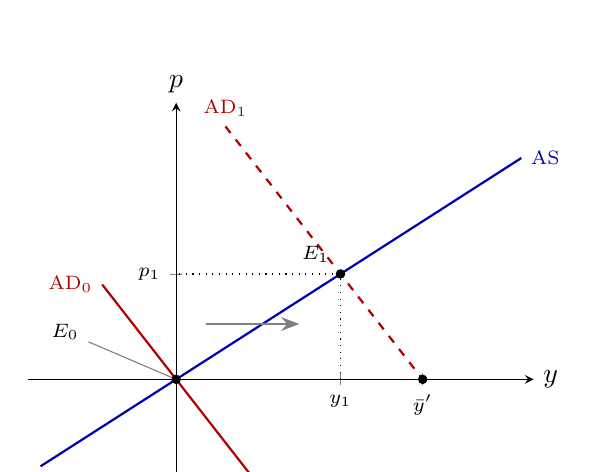
\begin{tikzpicture}
\begin{axis}[width=8cm,height=6.4cm,axis lines=middle,xmin=-0.6,xmax=1.45,ymin=-0.65,ymax=1.75,clip=false,
  xlabel={$y$},ylabel={$p$},xtick={0.6667,1},xticklabels={$y_1$,$\bar y'$},ytick={0.6667},yticklabels={$p_1$},
  every tick label/.append style={font=\scriptsize},x label style={anchor=west},y label style={anchor=south}]
\addplot[thick,blue!70!black,domain=-0.55:1.4]{x};
\addplot[thick,red!70!black,domain=-0.3:0.3]{-2*x};
\addplot[thick,red!70!black,dashed,domain=0.2:1.0]{2-2*x};
\node[font=\scriptsize,blue!70!black,anchor=west] at (axis cs:1.4,1.4){AS};
\node[font=\scriptsize,red!70!black,anchor=east] at (axis cs:-0.3,0.6){AD$_0$};
\node[font=\scriptsize,red!70!black,anchor=south] at (axis cs:0.2,1.6){AD$_1$};
\addplot[only marks,mark=*,mark size=1.5pt]coordinates{(0,0)(0.6667,0.6667)(1,0)};
\node[font=\scriptsize] (e0) at (axis cs:-0.45,0.3){$E_0$};
\draw[gray,thin](e0)--(axis cs:0,0);
\node[font=\scriptsize,anchor=south east] at (axis cs:0.66,0.68){$E_1$};
\draw[dotted](axis cs:0.6667,0)--(axis cs:0.6667,0.6667)--(axis cs:0,0.6667);
\draw[-{Stealth},thick,gray](axis cs:0.12,0.35)--(axis cs:0.5,0.35);
\end{axis}
\end{tikzpicture}\\
{\footnotesize Figure 4. News of higher $\bar a$ shifts AD right (it now passes through $(\bar y',\bar p)$ at $i=\rho$);
AS stays. $E_1$: $y_1-y_n=y_1-y_e>0$ and $p_1>p^e$. (Drawn for $\sigma=0.5$, $\kappa=1$, $\Gamma d\bar a=1$; the origin is
$(y_n,p^e)$.)}
\end{center}
\intuicao{Expectations about the future move demand today. Supply today has not changed, so the extra demand
can only be met by working harder with the same technology, and prices rise.}
\refbib{Benigno (2015) \S6.3, Fig.~8, pp.~511--513; \S5, eqs.~(20)--(21), pp.~509--511; \S4.2--\S4.4 ($y_n$, $y_e$), pp.~508--509.}
\rubrica{
\item AD shifts right, with the Euler/permanent-income reason: 0.3 pt.
\item AS does not move, because $y_n$ depends on current $a,\mu$ only: 0.2 pt.
\item $dy$ and $dp$: 0.2 pt.
\item Both gaps signed and used in the explanation: 0.2 pt. Welfare verdict with the reason: 0.1 pt.
\item Graph lines are inside the first two items (axes $y,p$; AD$_0$, AD$_1$, AS named; $E_0$, $E_1$; direction of the shift).
\item Shifting AS (treating the news as current productivity): max.\ 0.3 pt. Signs of $dy$, $dp$ inconsistent with the graph: $-0.2$.
}
\end{sol}

\sub{3.b}{1 point} Based on the previous item, explain intuitively what a monetary authority committed
to price stability should do after the news, by how much it must move its instrument, and what is the
economic cost of doing so. Show graphically the paths of $y$ and $p$ in the short and in the long run,
with and without that response. A commentator claims that ``whatever the central bank does, it must
give up either price stability or a closed output gap''. Evaluate the claim.
\resolespaco[7cm]
\begin{sol}
\begin{notacao}
\item As in 3.a. New: $r_n$, the natural real interest rate, the real rate that clears today's goods
market at natural output.
\end{notacao}
\passo{target}{Price stability: $p=p^e$. On AS \eqref{q3:AS} this requires $y=y_n$, and since
$y_n=y_e$ here, it also gives $y=y_e$.}
\passo{instrument}{AD must pass through $(y_n,p^e)=(0,p^e)$. Set $y=0$ and $p=p^e$ in \eqref{q3:ADr},
with $\bar y=\Gamma d\bar a$ from \eqref{q3a:dybar}:}
\begin{align*}
0 &= (\Gamma\,d\bar a)-\sigma(i-\rho)-\sigma(p^e-p^e)\\
0 &= \Gamma\,d\bar a-\sigma(i-\rho)\\
\sigma(i-\rho) &= \Gamma\,d\bar a.
\end{align*}
Divide by $\sigma$:
\begin{equation}
\boxed{i=\rho+\frac{\Gamma\,d\bar a}{\sigma}} \label{q3b:i}
\end{equation}
\textbf{Raise} $i$ by $\Gamma d\bar a/\sigma>0$. The natural real rate is
\begin{equation}
r_n=\rho+\sigma^{-1}(\bar y-y_n). \label{q3b:rn}
\end{equation}
Differentiate \eqref{q3b:rn} and substitute \eqref{q3a:dybar} and $dy_n=0$:
\begin{align*}
dr_n &= \sigma^{-1}\big[(\Gamma\,d\bar a)-(0)\big]\\
&= \frac{\Gamma\,d\bar a}{\sigma}.
\end{align*}
The rise in \eqref{q3b:i} is exactly the rise in $r_n$. The future is richer, so the real rate that clears today's goods market
at natural output is higher. AD returns to AD$_0$ in Figure 4.
\passo{cost}{\textbf{None} in terms of the two objectives: after the rise $y=y_n=y_e$ and $p=p^e$. The shock is
\emph{efficient}: it does not separate $y_n$ from $y_e$ (no mark-up moved), so one instrument closes both gaps
(divine coincidence). The commentator is wrong for this shock. A cut, the instinct to ``support the good
news'', would push output and prices further up.}
\passo{long run}{In period 2 all prices adjust and $y=\bar y'=\Gamma d\bar a$, $p=\bar p$, with or without the
response. The higher rate does not cancel the gain; it \emph{times} it: households wait for the productivity to
arrive instead of working beyond the efficient level today. The same response is right if the news is only
optimism; the model cannot tell the two apart in the short run.}
\begin{center}
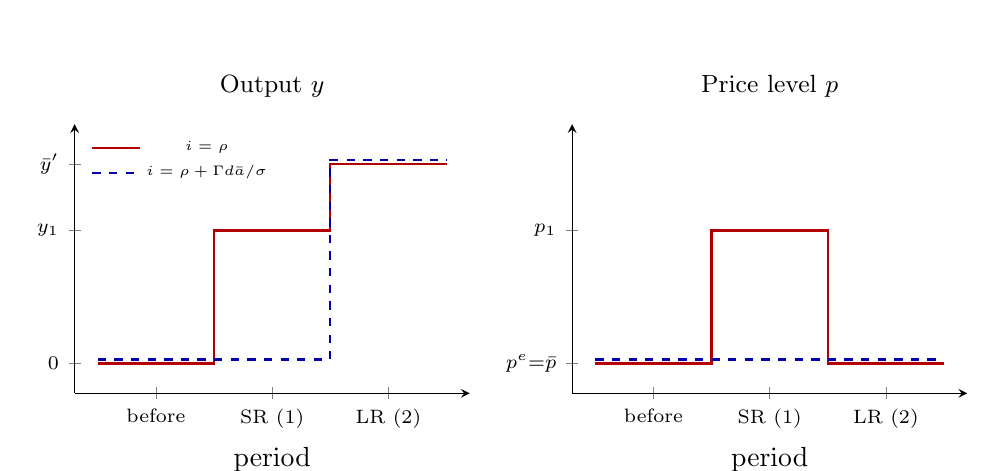
\begin{tikzpicture}
\begin{axis}[name=py,width=6.6cm,height=5cm,axis lines=left,xmin=-0.2,xmax=3.2,ymin=-0.15,ymax=1.2,
  xlabel={period},xtick={0.5,1.5,2.5},xticklabels={before,SR (1),LR (2)},ytick={0,0.6667,1},
  yticklabels={$0$,$y_1$,$\bar y'$},title={\small Output $y$},every tick label/.append style={font=\scriptsize},
  legend style={font=\tiny,draw=none,at={(0.02,0.98)},anchor=north west}]
\addplot[thick,red!70!black,const plot] coordinates {(0,0)(1,0.6667)(2,1)(3,1)};
\addplot[thick,blue!70!black,dashed,const plot] coordinates {(0,0.02)(1,0.02)(2,1.02)(3,1.02)};
\legend{$i=\rho$,$i=\rho+\Gamma d\bar a/\sigma$}
\end{axis}
\begin{axis}[at={(py.east)},anchor=west,xshift=1.3cm,width=6.6cm,height=5cm,axis lines=left,xmin=-0.2,xmax=3.2,
  ymin=-0.15,ymax=1.2,xlabel={period},xtick={0.5,1.5,2.5},xticklabels={before,SR (1),LR (2)},ytick={0,0.6667},
  yticklabels={$p^e{=}\bar p$,$p_1$},title={\small Price level $p$},every tick label/.append style={font=\scriptsize}]
\addplot[thick,red!70!black,const plot] coordinates {(0,0)(1,0.6667)(2,0)(3,0)};
\addplot[thick,blue!70!black,dashed,const plot] coordinates {(0,0.02)(3,0.02)};
\end{axis}
\end{tikzpicture}\\
{\footnotesize Figure 5. Solid: no response, a boom with a price surprise in the short run. Dashed: the rate rise
keeps $y=y_n=y_e$ and $p=p^e$ in the short run; in the long run both paths reach $\bar y'$ and $\bar p$.}
\end{center}
\intuicao{The central bank's job is to set the real rate to the one the economy would have with flexible prices.
Good news about the future raises that rate; tracking it is not ``fighting'' the news.}
\refbib{Benigno (2015) \S6.3, Fig.~8, pp.~511--513 (optimal response to expected productivity); \S5 ($r_n$); \S11, p.~522
(no trade-off when $y_n=y_e$).}
\rubrica{
\item Raise $i$, with the mechanism (AD back through $(y_n,p^e)$): 0.3 pt.
\item Size $\Gamma d\bar a/\sigma$, read as the rise in $r_n$: 0.2 pt.
\item Cost: none, both gaps closed, because the shock is efficient ($y_n=y_e$); claim rejected: 0.3 pt.
\item Paths SR/LR with and without the response: 0.2 pt (0.1 if the long run is missing).
\item Cutting $i$: max.\ 0.2 pt on the item. ``Cost: a recession'' (a trade-off asserted): max.\ 0.5 pt.
}
\gap{Prova 01, 3.a--3.b: which bar moves which curve; sign of the policy response to a pure AD shift; the cost
of a response when there is no trade-off.}
\end{sol}

\sub{3.c}{1 point} Suppose the monetary authority represents society's preferences by the quadratic
loss function, with parameter $\phi\geq0$,
\begin{equation}
L=\frac12\left(y-y_e\right)^2+\frac{\phi}{2\kappa}\left(p-p^e\right)^2 . \tag{LF}\label{q3:LF}
\end{equation}
In the same period as the news of item 3.a, the government temporarily raises a tax on firms' sales
revenue (an IPI-like tax), which raises the current mark-up by $d\mu>0$; the long-run mark-up $\bar\mu$
does not change. Derive the optimal monetary-policy rule (IT), find the optimal $y$, $p$ and $i$, and
show graphically the optimal policy. Discuss how your answer depends on $\phi$, separating the part of
the optimal response that answers the news from the part that answers the mark-up shock.
\resolespaco[8cm]
\begin{sol}
\begin{notacao}
\item As in 3.a--3.b. New: $\phi\ge0$, the weight on price surprises in \eqref{q3:LF}.
\item $m\equiv\frac{d\mu}{\sigma^{-1}+\eta}>0$: the fall in natural output caused by the tax.
$y_n'$: natural output after the tax.
\item $y^\ast$, $p^\ast$, $i^\ast$: optimal output, price level and interest rate; $O=(y^\ast,p^\ast)$.
\item $N$, $y_N$: the point on the new AS, and its output, reached when $i$ only offsets the news.
\end{notacao}
\passo{what the tax moves}{Differentiate \eqref{q3:YN} with respect to the current mark-up:}
\begin{equation}
y_n'=-\frac{d\mu}{\sigma^{-1}+\eta}=-m<0. \label{q3c:yn}
\end{equation}
Current natural output falls, so \textbf{AS shifts up/left} through $(y_n',p^e)$. $y_e$ in
\eqref{q3:ye} has no $\mu$: $y_e=0$ is unchanged. Now $y_n\neq y_e$: the tax is an
\emph{inefficient} shock. $\bar\mu$ is unchanged, so by \eqref{q3:ybar} the AD shift is only the
news ($\bar y=\Gamma d\bar a$, \eqref{q3a:dybar}).
\passo{AS is the constraint}{The central bank moves AD with $i$; for any point on AS there is an
$i$ that puts AD through it. AS, with $p^e$ preset, is what policy cannot move within the period:
it is the feasible set. So choose $y$ on AS and recover $i$ from AD. By \eqref{q3:AS} with
\eqref{q3c:yn}, the constraint is}
\begin{equation}
p-p^e=\kappa\,(y-y_n'). \label{q3c:AS}
\end{equation}
Substitute \eqref{q3c:AS} into \eqref{q3:LF}:
\begin{align}
L(y) &= \tfrac12(y-y_e)^2+\tfrac{\phi}{2\kappa}\big[\kappa\,(y-y_n')\big]^2\nonumber\\
&= \tfrac12(y-y_e)^2+\tfrac{\phi}{2\kappa}\kappa^2(y-y_n')^2\nonumber\\
&= \tfrac12(y-y_e)^2+\tfrac{\phi\kappa}{2}(y-y_n')^2 . \label{q3c:L}
\end{align}
\passo{targeting rule}{Differentiate \eqref{q3c:L} and set it to zero:}
\begin{equation}
\frac{dL}{dy}=(y-y_e)+\phi\kappa\,(y-y_n')=0. \label{q3c:foc}
\end{equation}
By \eqref{q3c:AS}, $\kappa(y-y_n')=p-p^e$. Substitute this into \eqref{q3c:foc}:
\begin{equation}
\boxed{(y-y_e)+\phi\,(p-p^e)=0}\qquad\text{(IT: a line through $(y_e,p^e)$ with slope $-1/\phi$).} \label{q3c:IT}
\end{equation}
SOC: from \eqref{q3c:L}, $d^2L/dy^2=1+\phi\kappa>0$.
\passo{optimal point}{Solve \eqref{q3c:foc} for $y$:}
\begin{align}
y(1+\phi\kappa) &= y_e+\phi\kappa\,y_n'\nonumber\\
y^\ast &= \frac{y_e+\phi\kappa\,y_n'}{1+\phi\kappa}. \label{q3c:ystar}
\end{align}
Substitute $y_e=0$ and \eqref{q3c:yn} into \eqref{q3c:ystar}:
\begin{align}
y^\ast &= \frac{(0)+\phi\kappa\,(-m)}{1+\phi\kappa}\nonumber\\
&= \boxed{-\frac{\phi\kappa}{1+\phi\kappa}\,m<0} \label{q3c:ystarm}
\end{align}
Substitute \eqref{q3c:ystarm} and \eqref{q3c:yn} into \eqref{q3c:AS}:
\begin{align}
p^\ast-p^e &= \kappa(y^\ast-y_n')\nonumber\\
&= \kappa\left[\left(-\frac{\phi\kappa}{1+\phi\kappa}\,m\right)-(-m)\right]\nonumber\\
&= \kappa\left(m-\frac{\phi\kappa\,m}{1+\phi\kappa}\right)\nonumber\\
&= \boxed{\frac{\kappa}{1+\phi\kappa}\,m>0}. \label{q3c:pstar}
\end{align}
Check in \eqref{q3c:IT}:
\begin{align*}
(y^\ast-y_e)+\phi(p^\ast-p^e) &= \left[\left(-\frac{\phi\kappa}{1+\phi\kappa}\,m\right)-(0)\right]
+\phi\left(\frac{\kappa}{1+\phi\kappa}\,m\right)\\
&= \frac{-\phi\kappa m+\phi\kappa m}{1+\phi\kappa}=0\ \checkmark
\end{align*}
The bank splits the shock: output below efficient \emph{and} prices above $p^e$.
\passo{optimal rate}{Evaluate AD \eqref{q3:ADr} at $(y^\ast,p^\ast)$, with $\bar y=\Gamma d\bar a$,
and solve for $i^\ast$:}
\begin{align}
(y^\ast) &= (\Gamma\,d\bar a)-\sigma(i^\ast-\rho)-\sigma\big((p^\ast)-p^e\big)\nonumber\\
\sigma(i^\ast-\rho) &= \Gamma\,d\bar a-y^\ast-\sigma(p^\ast-p^e)\nonumber\\
i^\ast &= \rho+\frac{\Gamma\,d\bar a-y^\ast}{\sigma}-(p^\ast-p^e). \label{q3c:igen}
\end{align}
Substitute \eqref{q3c:ystarm} and \eqref{q3c:pstar} into \eqref{q3c:igen}:
\begin{align}
i^\ast &= \rho+\frac{\Gamma\,d\bar a-\left(-\frac{\phi\kappa}{1+\phi\kappa}\,m\right)}{\sigma}
-\left(\frac{\kappa}{1+\phi\kappa}\,m\right)\nonumber\\
&= \rho+\frac{\Gamma\,d\bar a}{\sigma}+\frac{\phi\kappa m}{\sigma(1+\phi\kappa)}-\frac{\kappa m}{1+\phi\kappa}. \label{q3c:i4}
\end{align}
Put the last two terms of \eqref{q3c:i4} over the common denominator $\sigma(1+\phi\kappa)$:
\begin{equation}
\boxed{i^\ast=\rho+\underbrace{\frac{\Gamma\,d\bar a}{\sigma}}_{\text{news}}
+\underbrace{\frac{\kappa\,m\,(\phi-\sigma)}{\sigma(1+\phi\kappa)}}_{\text{mark-up}}} \label{q3c:istar}
\end{equation}
\passo{the news part does not depend on $\phi$}{The news moves neither $y_n$ nor $y_e$, so by
\eqref{q3c:ystar} it does not move the optimal point $O=(y^\ast,p^\ast)$ on AS. The bank simply
undoes the AD shift, $di=\Gamma d\bar a/\sigma$ in \eqref{q3c:istar}, for \emph{any} $\phi$, exactly
as in \eqref{q3b:i}.}
\passo{the mark-up part depends on $\phi$ against $\sigma$}{Substitute the news-offset rate
\eqref{q3b:i} and $\bar y=\Gamma d\bar a$ into AD \eqref{q3:ADr}: AD is back at AD$_0$. Then
substitute \eqref{q3c:AS} for $p-p^e$ to find the point $N$:}
\begin{align}
y &= (\Gamma\,d\bar a)-\sigma\left(\frac{\Gamma\,d\bar a}{\sigma}\right)-\sigma(p-p^e)\nonumber\\
&= -\sigma(p-p^e)\nonumber\\
y &= -\sigma\big[\kappa\,(y-y_n')\big]\nonumber\\
y_N &= \frac{\sigma\kappa}{1+\sigma\kappa}\,y_n'. \label{q3c:yN}
\end{align}
Subtract \eqref{q3c:yN}, with $y_n'=-m$, from \eqref{q3c:ystarm}:
\begin{align}
y^\ast-y_N &= \left(-\frac{\phi\kappa}{1+\phi\kappa}\,m\right)-\frac{\sigma\kappa}{1+\sigma\kappa}\,(-m)\nonumber\\
&= -\frac{\phi\kappa m}{1+\phi\kappa}+\frac{\sigma\kappa m}{1+\sigma\kappa}\nonumber\\
&= \frac{\kappa m(\sigma-\phi)}{(1+\phi\kappa)(1+\sigma\kappa)}. \label{q3c:diff}
\end{align}
If $\phi>\sigma$ (the IT line is flatter than AD), \eqref{q3c:diff} is negative: the bank raises $i$
further and accepts a deeper output loss for less price movement; if $\phi<\sigma$ it raises $i$ by
less than the news alone requires. Limits of \eqref{q3c:ystarm}, \eqref{q3c:pstar} and
\eqref{q3c:istar}:
\begin{align*}
\phi\to\infty\ \text{(strict price stability)}:&\quad y^\ast=y_n',\quad p^\ast=p^e,\quad
i^\ast=\rho+\frac{\Gamma d\bar a+m}{\sigma},\\
\phi=0:&\quad y^\ast=y_e,\quad p^\ast=p^e+\kappa m,\quad i^\ast=\rho+\frac{\Gamma d\bar a}{\sigma}-\kappa m.
\end{align*}
\passo{trade-off}{Unlike 3.b there is a trade-off: $y_n'\neq y_e$, so no rate closes both gaps;
$\phi$ chooses where on AS to sit.}
\begin{center}\begin{minipage}{\linewidth}\centering
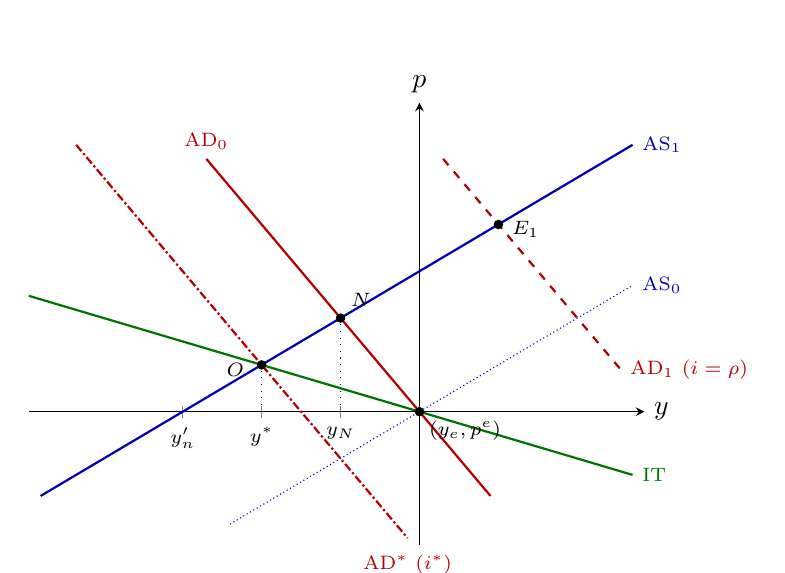
\begin{tikzpicture}
\begin{axis}[width=9.4cm,height=7.2cm,axis lines=middle,xmin=-1.65,xmax=0.95,ymin=-0.95,ymax=2.2,clip=false,
  xlabel={$y$},ylabel={$p$},xtick={-1,-0.6667,-0.3333},xticklabels={$y_n'$,$y^\ast$,$y_N$},ytick=\empty,
  every tick label/.append style={font=\scriptsize},x label style={anchor=west},y label style={anchor=south}]
\addplot[densely dotted,blue!70!black,domain=-0.8:0.9]{x};
\addplot[thick,blue!70!black,domain=-1.6:0.9]{x+1};
\addplot[thick,green!45!black,domain=-1.65:0.9]{-x/2};
\addplot[thick,red!70!black,dashed,domain=0.1:0.85]{2-2*x};
\addplot[thick,red!70!black,domain=-0.9:0.3]{-2*x};
\addplot[thick,red!70!black,densely dashdotted,domain=-1.45:-0.05]{-1-2*x};
\node[font=\scriptsize,blue!70!black,anchor=west] at (axis cs:0.9,0.9){AS$_0$};
\node[font=\scriptsize,blue!70!black,anchor=west] at (axis cs:0.9,1.9){AS$_1$};
\node[font=\scriptsize,green!45!black,anchor=west] at (axis cs:0.9,-0.45){IT};
\node[font=\scriptsize,red!70!black,anchor=west] at (axis cs:0.85,0.3){AD$_1$ ($i=\rho$)};
\node[font=\scriptsize,red!70!black,anchor=south] at (axis cs:-0.9,1.8){AD$_0$};
\node[font=\scriptsize,red!70!black,anchor=north] at (axis cs:-0.05,-0.95){AD$^\ast$ ($i^\ast$)};
\addplot[only marks,mark=*,mark size=1.5pt]coordinates{(0.3333,1.3333)(-0.3333,0.6667)(-0.6667,0.3333)(0,0)};
\node[font=\scriptsize,anchor=west] at (axis cs:0.35,1.3){$E_1$};
\node[font=\scriptsize,anchor=south west] at (axis cs:-0.33,0.68){$N$};
\node[font=\scriptsize,anchor=east] at (axis cs:-0.7,0.3){$O$};
\node[font=\scriptsize,anchor=north west] at (axis cs:0,0){$(y_e,p^e)$};
\draw[dotted](axis cs:-0.6667,0)--(axis cs:-0.6667,0.3333);
\draw[dotted](axis cs:-0.3333,0)--(axis cs:-0.3333,0.6667);
\end{axis}
\end{tikzpicture}\\
{\footnotesize Figure 6. The tax shifts AS from AS$_0$ to AS$_1$ (through $(y_n',p^e)$); the news shifts AD from AD$_0$ to
AD$_1$. With $i=\rho$ the economy is at $E_1$. Offsetting the news alone brings AD back to AD$_0$ and the economy to
$N$. The optimum $O$ is where AS$_1$ meets the IT line; drawn for $\phi=2>\sigma=0.5$, so the bank raises $i$ beyond
the news offset, to AD$^\ast$. ($\kappa=1$, $\Gamma d\bar a=m=1$.)}
\end{minipage}\end{center}
\intuicao{Two shocks, two different jobs. The news is a demand shock with no trade-off: offset it fully. The tax is a
cost shock that drives a wedge between natural and efficient output: no rate fixes both gaps, so the convex loss
spreads the miss, and $\phi$ says how much of it goes into prices.}
\refbib{Benigno (2015) \S11, eqs.~(33)--(35), Fig.~14, pp.~521--523; \S7, Fig.~9, pp.~513--514 (mark-up shocks; taxes in
$1+\mu$); \S4.4, p.~509.}
\rubrica{
\item AS shifts up/left, $y_e$ does not move, AD shift from the news only: 0.15 pt.
\item Why AS is the constraint; substitution into $L$: 0.15 pt.
\item Targeting rule $(y-y_e)+\phi(p-p^e)=0$ from $dL/dy=0$: 0.2 pt.
\item $y^\ast$, $p^\ast$: 0.15 pt. $i^\ast$ with its two components: 0.15 pt.
\item Role of $\phi$: news part independent of $\phi$; mark-up part signed by $\phi-\sigma$; a limit case: 0.1 pt.
\item Graph (AS$_1$, IT, AD before/after, $O$ labelled): 0.1 pt.
\item Differentiating in $i$ with AD as the constraint, or targeting $y_n$ instead of $y_e$: max.\ 0.4 pt. Claiming the whole
response (news included) depends on $\phi$ versus $\sigma$: max.\ 0.6 pt.
}
\gap{Prova 01, 3.c: $dL/dy=0$ along AS not used; the response to news wrongly made to depend on $\phi$.}
\end{sol}

\ifsolucoes\else
\vfill
\begin{center}\footnotesize\textit{End of exam.}\end{center}
\fi

\end{document}
"
% Check fonts: pdffonts <file>.pdf  (all Type 1).
% Every closed form and number in the key: python simulado_codigo/check_simulado_04.py
% Solution format (rules/00_estilo_avaliacao.md §4): each solution opens with a Notation list;
% every equation used later is numbered and cited with \eqref; one operation per displayed line.
% Numbering: Q1 solutions use (G1), (G2)...; Q2 keeps the statement's (1)-(4) and continues from
% (5); Q3 keeps the statement's (AD), (AS), (YN), (LF) and continues the numeric sequence.
% =============================================================================
\documentclass[11pt,a4paper]{article}
\usepackage[utf8]{inputenc}
\usepackage[T1]{fontenc}
\usepackage{lmodern}   % Type 1 vector fonts (replaces PK bitmaps)
\usepackage{cmap}      % ToUnicode CMap -> copyable text and accents
\usepackage[english]{babel}
\usepackage{amsmath,amssymb,amsfonts}
\usepackage[a4paper,margin=2.2cm]{geometry}
\usepackage{enumitem}
\usepackage{fancyhdr}
\usepackage{comment}
% Private cut file per build (sibling sources build in this folder). comment.sty resets
% \CommentCutFile from \DefaultCutFileName at every included environment, so redefine that.
\def\DefaultCutFileName{\def\CommentCutFile{\jobname.cut}}
\usepackage{xcolor}
\usepackage{microtype}
\usepackage{booktabs}
\usepackage{needspace}
\usepackage{pgfplots}
\pgfplotsset{compat=1.18}
\usetikzlibrary{arrows.meta}

% ====================== CONFIGURATION ======================
\newif\ifsolucoes
\ifdefined\withsolutions\solucoestrue\else\solucoesfalse\fi

\newcommand{\disciplina}{Macroeconomics I --- MPE Insper}
\newcommand{\listatema}{Mock Exam 4}

% ====================== MACHINERY ======================
\ifsolucoes\includecomment{sol}\else\excludecomment{sol}\fi

\pagestyle{fancy}\fancyhf{}
\lhead{\footnotesize\disciplina}
\rhead{\footnotesize \listatema\ifsolucoes{} --- Solutions and Rubric\fi}
\cfoot{\footnotesize\thepage}
\renewcommand{\headrulewidth}{0.3pt}
\setlength{\headheight}{14pt}
\setlist{topsep=2pt,itemsep=2pt}

% \questao{number}{points}{statement}
\newcommand{\questao}[3]{\Needspace{12\baselineskip}\bigskip\noindent
  {\large\bfseries\color{blue!55!black}Question #1}\ \textbf{(#2 points)}\par\smallskip\noindent #3\par}
% \item-like heading: \sub{2.a}{1 point}
\newcommand{\sub}[2]{\Needspace{8\baselineskip}\par\medskip\noindent\textbf{#1 (#2)}~}
\newcommand{\resolespaco}[1][6cm]{\ifsolucoes\else\par\textit{Solution:}\vspace{#1}\par\fi}
\newcommand{\passo}[2]{\par\smallskip\noindent\textbf{Step --- #1.}~#2}
\newcommand{\intuicao}[1]{\par\smallskip\noindent\textit{Intuition.}~#1}
\newcommand{\refbib}[1]{\par\smallskip\noindent{\footnotesize\color{black!60}\textbf{Ref:} #1}}
\newcommand{\gap}[1]{\par\smallskip\noindent{\footnotesize\color{red!55!black}\textbf{Gap targeted:} #1}}
\newcommand{\trap}[1]{\par\smallskip\noindent{\small\color{red!55!black}\#~#1}}
\newcommand{\rubrica}[1]{\par\smallskip\noindent\textbf{Grading rubric.}\begin{itemize}[leftmargin=1.4em,topsep=1pt]#1\end{itemize}}
\newenvironment{notacao}{\par\smallskip\noindent\textbf{Notation.}\begin{itemize}[leftmargin=1.4em,topsep=1pt,itemsep=0pt]\small}{\end{itemize}}
\allowdisplaybreaks

% =============================================================================
\begin{document}
\begin{center}
  {\Large\bfseries \disciplina}\\[2pt]
  {\large \listatema\ (Simulado 4) --- 2026, 3rd term}\ifsolucoes\\[2pt]\textit{Solutions and Grading Rubric}\fi
\end{center}
\vspace{2pt}

{\footnotesize\noindent\textbf{Instructions.} Three questions, 10 points in total. Suggested time:
2 hours, closed book, non-programmable calculator allowed. Show every step: a number or a formula
without the argument that produces it earns little. When an item says \emph{explain},
\emph{justify} or \emph{show graphically}, the explanation and the graph are graded on their own
lines: label the axes and every curve, mark the initial and the new point, and indicate the
direction of every shift. Where an item lists several approaches or several choice variables,
answer \emph{each} of them. Box your final answers. Notation: Kurlat (2020) in Questions 1--2,
Benigno (2015) in Question 3.\par}

% =============================================================================
\renewcommand{\theequation}{G\arabic{equation}}% Q1 solution equations: (G1), (G2)...
\questao{1}{1.5}{A simplified economy has, at first, no government. Values are in R\$ million
for one year. A coffee farm in Minas Gerais (Firm F) grows beans worth 400 and sells all of them
to a roastery (Firm R); F uses no inputs and pays 250 in wages. Firm R buys the 400 of beans and
imports packaging worth 100 from abroad; it sells roasted coffee worth 700 to domestic households
and worth 200 to foreign buyers, and pays 300 in wages. Each firm keeps whatever is left as profit.}

\sub{1.a}{0.5 point} Calculate the GDP of this economy by the product, the income and the
expenditure approaches, explaining precisely the concept used in each. Explain why the imported
packaging does not count in GDP, although Firm R used it to produce.
\resolespaco[5.5cm]
\begin{sol}
\begin{notacao}
\item F, R: the coffee farm and the roastery. All values in R\$ million for one year.
\item $VA_j\ge0$: value added of firm $j$, its production minus the intermediate inputs it uses up.
\item $W_j\ge0$: wages paid by firm $j$. $\Pi_j$: its profit (operating surplus), whatever is left
after wages; it can be of either sign.
\item $C$, $I$, $G$: household consumption, investment and government purchases (final domestic
uses). $X\ge0$, $M\ge0$: exports and imports. In 1.a, $I=G=0$.
\end{notacao}
\passo{0, the definitions used below}{GDP is the market value of the \emph{final} goods and
services produced in the territory in the year. It is computed three ways, which must agree:}
\begin{align}
\text{GDP} &= \textstyle\sum_j VA_j, \label{q1:prod}\\
VA_j &= \text{production}_j-\text{intermediate inputs}_j, \label{q1:va}\\
\Pi_j &= VA_j-W_j, \label{q1:profit}\\
\text{GDP} &= \textstyle\sum_j (W_j+\Pi_j), \label{q1:inc}\\
\text{GDP} &= C+I+G+X-M. \label{q1:exp}
\end{align}
\passo{product (value added)}{F uses no inputs; R uses the beans and the imported packaging.
Using \eqref{q1:va} for each firm:}
\begin{align}
VA_F &= 400-0=400, \label{q1a:vaF}\\
VA_R &= (700+200)-400-100\nonumber\\
&= 900-500\nonumber\\
&= 400. \label{q1a:vaR}
\end{align}
Summing \eqref{q1a:vaF} and \eqref{q1a:vaR} with \eqref{q1:prod}:
\begin{equation}
\text{GDP}=400+400=\boxed{800}. \label{q1a:gdp}
\end{equation}
\passo{income (factor payments)}{Profit is what is left of value added after wages. Using
\eqref{q1:profit} with \eqref{q1a:vaF} and \eqref{q1a:vaR}:}
\begin{align}
\Pi_F &= 400-250=150, \label{q1a:piF}\\
\Pi_R &= 400-300=100. \label{q1a:piR}
\end{align}
Add wages and profits, then apply \eqref{q1:inc}:
\begin{align*}
W_F+W_R &= 250+300=550,\\
\Pi_F+\Pi_R &= 150+100=250,\\
\text{GDP} &= 550+250=\boxed{800}.
\end{align*}
\passo{expenditure (final uses)}{The final uses are $C=700$, $I=0$, $G=0$, $X=200$ and
$M=100$. By \eqref{q1:exp}:}
\[
\text{GDP}=700+0+0+200-100=\boxed{800}.
\]
\passo{imports}{The packaging was produced abroad: its 100 is \emph{foreign} value added. In the
product approach it is an intermediate input of R and is subtracted from R's production in
\eqref{q1a:vaR}. In the expenditure approach \eqref{q1:exp}, $C$ and $X$ are measured at purchaser
prices and already contain the packaging, so $-M$ takes it back out. GDP measures what is produced
\emph{in the territory}.}
\trap{Adding sales, $400+900=1300$, counts the beans twice (once as F's sale, once inside R's price) and
counts foreign packaging. The three approaches agree because they are three ways of adding up the same
value added.}
\intuicao{Every real that a final buyer pays for coffee ends up as somebody's income: F's workers and
owners, R's workers and owners, or the foreign packaging producer. Take the foreigner out and the three
columns must match.}
\refbib{Kurlat \S1.1, pp.~15--21 (value added, the three approaches, imports).}
\rubrica{
\item Each approach with the right concept and the number 800: 0.15 pt each (0.45).
\item Why imports are excluded (foreign value added; $-M$ corrects purchaser prices): 0.05 pt.
\item Only one approach, number right: max.\ 0.2 pt. Summing sales (1300) or forgetting $-M$ (900): 0 for that line.
}
\end{sol}

\sub{1.b}{0.5 point} Suppose instead that in the same year households buy only 600 of roasted
coffee. Firm R produces exactly as before and keeps the remaining roasted coffee in its warehouse at
the end of the year, valued at its selling price. Nothing else changes. Calculate, justifying, the
GDP by the product, income and expenditure approaches, compare it with the value in 1.a and explain
what the comparison indicates. Then explain what the sale of that stock to households in the
following year adds to the following year's GDP, other things equal.
\resolespaco[6cm]
\begin{sol}
\begin{notacao}
\item As in 1.a. New: $\Delta\text{inventories}$, the change in R's stock of unsold roasted coffee
during the year, valued at its selling price. It is part of $I$ and can be negative (a drawdown).
\end{notacao}
\passo{what changed}{R's production is unchanged; only its destination moved: households,
exports, and the part left unsold in the warehouse.}
\begin{equation}
\text{production}_R=600+200+100=900. \label{q1b:prodR}
\end{equation}
An unsold good that was produced is a \textbf{change in inventories}, a component of investment:
\begin{equation}
I=\Delta\text{inventories}=100. \label{q1b:inv}
\end{equation}
\passo{product}{F is unchanged, $VA_F=400$ by \eqref{q1a:vaF}. Using \eqref{q1:va} with
\eqref{q1b:prodR}:}
\begin{align*}
VA_R &= 900-400-100\\
&= 400.
\end{align*}
By \eqref{q1:prod}, GDP $=400+400=\boxed{800}$.
\passo{income}{R's operating surplus is measured on production, the stock valued at 100. Using
\eqref{q1:profit}:}
\begin{align*}
\Pi_R &= 900-500-300\\
&= 100.
\end{align*}
Wages are $250+300=550$ and profits $150+100=250$, with $\Pi_F$ from \eqref{q1a:piF}. By
\eqref{q1:inc}, GDP $=550+250=\boxed{800}$.
\passo{expenditure}{Now $C=600$, $I=100$ from \eqref{q1b:inv}, $G=0$, $X=200$, $M=100$. By
\eqref{q1:exp}:}
\[
\text{GDP}=600+100+0+200-100=\boxed{800}.
\]
\passo{comparison}{GDP is the same as \eqref{q1a:gdp}: \textbf{GDP measures production, not sales}.
Only the composition of final demand moved, $C\downarrow100$ and $I\uparrow100$. A firm that cannot
sell is recorded as having invested in its own stock (involuntary, in this case).}
\passo{next year}{Households buy the 100 from stock, so $C$ rises by 100 and inventory investment
is $-100$ (a drawdown). The net contribution to next year's GDP, by \eqref{q1:exp}:}
\begin{align*}
\Delta C &= +100,\\
\Delta I=\Delta\text{inventories} &= -100,\\
\Delta\text{GDP} &= 100-100=\boxed{0}.
\end{align*}
The coffee was counted in the year it was produced; counting it again when sold would double-count it.
\intuicao{Inventories are the entry that makes the expenditure column add up when sales and production
differ. Without it the expenditure side would read $600+200-100=700\neq800$.}
\refbib{Kurlat \S1.1, p.~18 (inventories and their drawdown), pp.~15--21.}
\rubrica{
\item Three approaches with 800 and the inventory entry in $I$: 0.1 pt each (0.3).
\item Comparison: production vs sales, $C$ replaced by $I$: 0.1 pt.
\item Next year: $+C$, $-I$, net zero, with the reason: 0.1 pt.
\item GDP $=700$ (unsold output treated as not produced): max.\ 0.1 pt. One approach only: max.\ 0.25 pt.
}
\end{sol}

\sub{1.c}{0.5 point} Return to the situation of 1.a. The government now collects a lump-sum tax
of 200 from households and uses it to: (i) pay 120 in wages to nurses in public clinics, which treat
patients free of charge; (ii) buy 30 of imported medicines, handed out free at those clinics;
(iii) pay 50 in cash transfers to low-income families (Bolsa Fam\'ilia). Households' purchases of
roasted coffee stay at 700 and nothing else changes. Calculate, justifying, the GDP by the product,
income and expenditure approaches, compare it with 1.a and explain what the comparison indicates.
Explain why GDP does not rise by 200.
\resolespaco[6.5cm]
\begin{sol}
\begin{notacao}
\item As in 1.a. New: the public clinics as a producer, with value added $VA_{\text{clinics}}$.
\item $T=200$: the lump-sum tax. $TR=50$: the cash transfers. Both are flows between households and
government with nothing produced in exchange.
\end{notacao}
\passo{valuing a free service}{Public health care has no market price, so its output is valued
\textbf{at cost}, wages plus inputs:}
\begin{equation}
\text{output}_{\text{clinics}}=120+30=150. \label{q1c:out}
\end{equation}
The medicines are an intermediate input of the clinics. Using \eqref{q1:va} with \eqref{q1c:out}:
\begin{equation}
VA_{\text{clinics}}=150-30=120. \label{q1c:va}
\end{equation}
\passo{product}{Sum \eqref{q1a:vaF}, \eqref{q1a:vaR} and \eqref{q1c:va} with \eqref{q1:prod}:}
\begin{equation}
\text{GDP}=400+400+120=\boxed{920}. \label{q1c:gdp}
\end{equation}
\passo{income}{The clinics have no operating surplus: output is defined as cost, so by
\eqref{q1:profit} their profit is $120-120=0$. Adding up and applying \eqref{q1:inc}:}
\begin{align*}
\text{wages} &= 250+300+120=670,\\
\text{profits} &= 150+100+0=250,\\
\text{GDP} &= 670+250=\boxed{920}.
\end{align*}
\passo{expenditure}{$G=150$ is the clinics' output \eqref{q1c:out}, consumed on behalf of
households. Imports now include the medicines:}
\[
M=100+30=130.
\]
With $C=700$, $I=0$ and $X=200$, by \eqref{q1:exp}:
\[
\text{GDP}=700+0+150+200-130=\boxed{920}.
\]
\passo{what is left out, and why}{\textbf{The tax} (200) is a transfer from households to the
government, not a payment for a good: it is in no column. \textbf{Transfers} (50) buy nothing in
exchange: they are not in $G$ and not factor income (if the families spent them, the spending would
appear in $C$; here $C$ is unchanged by assumption). \textbf{Imported medicines} (30) enter $G$ but are
removed by $-M$: foreign value added.}
\passo{comparison}{Subtract \eqref{q1a:gdp} from \eqref{q1c:gdp}:}
\[
\Delta\text{GDP}=920-800=\boxed{120},
\]
the value added of public health care \eqref{q1c:va}, i.e.\ the nurses' wages. Not by 200 (the tax
is a financing flow), not by 150 (30 of $G$ is imported), not by 50 (transfers are redistribution).
\intuicao{Valuing government output at cost has a consequence: measured public-sector value added equals
its wage bill. If the nurses treated twice as many patients for the same pay, GDP would not record it.}
\refbib{Kurlat \S1.1, p.~20 (Example 1.7, government output at cost; Example 1.8, transfers), pp.~15--21.}
\rubrica{
\item Three approaches with 920, clinics' output at cost and $VA=120$: 0.1 pt each (0.3).
\item Tax, transfers and imported medicines each correctly excluded, with the reason: 0.1 pt.
\item Comparison: $+120$ is the nurses' value added: 0.1 pt.
\item Transfers counted in $G$ (GDP 970) or tax counted (1000): max.\ 0.2 pt. Medicines not netted by $M$ (950): $-0.1$.
}
\gap{Prova 01, 1.b--1.c: the three approaches were asked and only one was given; the classification of a
final use (there: software as investment; here: inventories as investment, clinics' output as $G$).}
\end{sol}

% =============================================================================
\questao{2}{5.5}{Consider an economy described by the Solow model, in which the aggregate variables
satisfy:
\begin{align}
Y_t &= K_t^{\alpha}(A_tL_t)^{1-\alpha}, \tag{1}\label{q2:Y}\\
K_{t+1} &= (1-\delta)K_t+s\,Y_t, \tag{2}\label{q2:K}\\
L_{t+1} &= (1+n)L_t, \tag{3}\label{q2:L}\\
A_{t+1} &= (1+g)A_t, \tag{4}\label{q2:A}
\end{align}
with $\{\alpha,\delta,s\}\in(0,1)$ and $n,g\geq0$.}
\setcounter{equation}{4}\renewcommand{\theequation}{\arabic{equation}}% Q2-Q3 continue from (5)

\sub{2.a}{1 point} Define the stationary variables, per efficiency unit of labour, with a tilde
($\tilde k_t$, $\tilde y_t$), and find an expression for $\tilde k_{t+1}/\tilde k_t$ and then the
steady-state value of $\tilde k$, denoted $\tilde k_{SS}$. Show the steady state graphically. Along
the steady state, at what rates do output per worker $y_t=Y_t/L_t$ and aggregate output $Y_t$ grow?
Justify, and explain why output per worker is not a stationary variable here.
\resolespaco[7cm]
\begin{sol}
\begin{notacao}
\item $Y_t$, $K_t$, $C_t>0$: aggregate output, capital and consumption. $L_t>0$: number of workers.
\item $A_t>0$: labour-augmenting technology; $A_tL_t$ is labour in efficiency units.
\item $\alpha\in(0,1)$: elasticity of output with respect to capital (capital's income share).
$\delta\in(0,1)$: depreciation rate. $s\in(0,1)$: saving rate. $n\ge0$: labour-force growth rate.
$g\ge0$: growth rate of technology.
\item $\tilde k_t$, $\tilde y_t$, $\tilde c_t>0$: capital, output and consumption per efficiency unit
of labour. $k_t=K_t/L_t$, $y_t=Y_t/L_t$: per worker.
\item $\xi\equiv(1+g)(1+n)-(1-\delta)>0$: break-even investment per unit of $\tilde k$ (defined in
step 3). $\tilde k_{SS}$, $\tilde y_{SS}$: steady-state values.
\end{notacao}
\passo{stationary variables}{Technology and labour both grow, so the variables that settle down are
those per efficiency unit:}
\begin{equation}
\tilde k_t\equiv\frac{K_t}{A_tL_t},\qquad \tilde y_t\equiv\frac{Y_t}{A_tL_t},\qquad
\tilde c_t\equiv\frac{C_t}{A_tL_t}. \label{q2a:def}
\end{equation}
Divide \eqref{q2:Y} by $A_tL_t$ and use \eqref{q2a:def}:
\begin{align}
\tilde y_t &= \frac{K_t^{\alpha}(A_tL_t)^{1-\alpha}}{A_tL_t}\nonumber\\
&= K_t^{\alpha}(A_tL_t)^{-\alpha}\nonumber\\
&= \left(\frac{K_t}{A_tL_t}\right)^{\alpha}\nonumber\\
&= \tilde k_t^{\alpha}. \label{q2a:y}
\end{align}
\passo{law of motion}{Multiply \eqref{q2:A} by \eqref{q2:L}:}
\begin{align}
A_{t+1}L_{t+1} &= \big[(1+g)A_t\big]\big[(1+n)L_t\big]\nonumber\\
&= (1+g)(1+n)A_tL_t. \label{q2a:AL}
\end{align}
Divide \eqref{q2:K} by \eqref{q2a:AL}. The second line splits the fraction, the third uses
\eqref{q2a:def}, the fourth \eqref{q2a:y}:
\begin{align}
\tilde k_{t+1} &= \frac{(1-\delta)K_t+sY_t}{(1+g)(1+n)A_tL_t}\nonumber\\
&= \frac{(1-\delta)\frac{K_t}{A_tL_t}+s\frac{Y_t}{A_tL_t}}{(1+g)(1+n)}\nonumber\\
&= \frac{(1-\delta)\tilde k_t+s\tilde y_t}{(1+g)(1+n)}\nonumber\\
&= \frac{(1-\delta)\tilde k_t+s\tilde k_t^{\alpha}}{(1+g)(1+n)}. \label{q2a:lom}
\end{align}
Divide \eqref{q2a:lom} by $\tilde k_t$:
\begin{equation}
\boxed{\frac{\tilde k_{t+1}}{\tilde k_t}=\frac{1-\delta+s\,\tilde k_t^{\alpha-1}}{(1+g)(1+n)}} \label{q2a:ratio}
\end{equation}
\passo{steady state}{Set \eqref{q2a:ratio} equal to 1 and isolate the term in $\tilde k$:}
\begin{align*}
1 &= \frac{1-\delta+s\tilde k^{\alpha-1}}{(1+g)(1+n)}\\
(1+g)(1+n) &= 1-\delta+s\tilde k^{\alpha-1}\\
s\tilde k^{\alpha-1} &= (1+g)(1+n)-(1-\delta).
\end{align*}
Call the right side $\xi$; expanding the product,
\begin{equation}
\xi\equiv(1+g)(1+n)-(1-\delta)=n+g+ng+\delta\ (\approx n+g+\delta). \label{q2a:xi}
\end{equation}
Using \eqref{q2a:xi}:
\begin{align*}
s\tilde k^{\alpha-1} &= \xi\\
\tilde k^{1-\alpha} &= \frac{s}{\xi}.
\end{align*}
Raise both sides to the power $1/(1-\alpha)$:
\begin{equation}
\boxed{\tilde k_{SS}=\left(\frac{s}{(1+g)(1+n)-(1-\delta)}\right)^{\frac{1}{1-\alpha}}} \label{q2a:kss}
\end{equation}
Evaluate \eqref{q2a:y} at \eqref{q2a:kss}, writing its denominator as $\xi$ by \eqref{q2a:xi}:
\begin{align}
\tilde y_{SS} &= \tilde k_{SS}^{\alpha}\nonumber\\
&= \left[\left(\frac{s}{\xi}\right)^{\frac{1}{1-\alpha}}\right]^{\alpha}\nonumber\\
&= \left(\frac{s}{\xi}\right)^{\frac{\alpha}{1-\alpha}}. \label{q2a:yss}
\end{align}
Multiplying the condition $s\tilde k^{\alpha-1}=\xi$ by $\tilde k$ gives the steady state as
investment equal to break-even investment:
\begin{equation}
s\tilde k_{SS}^{\alpha}=\xi\,\tilde k_{SS}. \label{q2a:break}
\end{equation}
\passo{stability}{In \eqref{q2a:ratio}, $\alpha-1<0$, so $\tilde k_{t+1}/\tilde k_t$ falls as
$\tilde k_t$ rises: it is $>1$ below $\tilde k_{SS}$ and $<1$ above. The positive steady state is
unique and every $\tilde k_0>0$ converges to it. Graphically (Figure 1): investment per efficiency
unit $s\tilde k^{\alpha}$ against break-even investment $\xi\tilde k$, the two sides of
\eqref{q2a:break}; $\xi$ is the amount needed to equip the new workers ($n$), the new efficiency
units ($g$) and to replace depreciation ($\delta$).}
\passo{growth rates}{In the steady state $\tilde y=\tilde y_{SS}$ is constant. Invert
\eqref{q2a:def}:}
\begin{align}
y_t &= \frac{Y_t}{L_t}=A_t\,\tilde y_{SS}, \label{q2a:ypw}\\
Y_t &= A_tL_t\,\tilde y_{SS}. \label{q2a:Yagg}
\end{align}
Take ratios of consecutive periods, using \eqref{q2:A} in \eqref{q2a:ypw} and \eqref{q2a:AL} in
\eqref{q2a:Yagg}:
\begin{align*}
\frac{y_{t+1}}{y_t} &= \frac{A_{t+1}\,\tilde y_{SS}}{A_t\,\tilde y_{SS}}\\
&= \frac{\big[(1+g)A_t\big]\tilde y_{SS}}{A_t\,\tilde y_{SS}}\\
&= 1+g &&\Rightarrow\ y_t\text{ grows at }\boxed{g},\\
\frac{Y_{t+1}}{Y_t} &= \frac{A_{t+1}L_{t+1}\,\tilde y_{SS}}{A_tL_t\,\tilde y_{SS}}\\
&= \frac{\big[(1+g)(1+n)A_tL_t\big]\tilde y_{SS}}{A_tL_t\,\tilde y_{SS}}\\
&= (1+g)(1+n) &&\Rightarrow\ Y_t\text{ grows at }\boxed{(1+g)(1+n)-1=g+n+gn}.
\end{align*}
The same holds for $k_t=K_t/L_t$ ($g$) and $K_t$ ($g+n+gn$); $K/Y$ is constant.
\passo{why $y$ is not stationary}{Each period every worker supplies $1+g$ times more efficiency units.
Capital per worker must grow at $g$ just to keep pace, so per-worker variables have a trend; dividing by
$A_tL_t$ removes it. Long-run growth of $y$ comes only from $g$, which the model takes as given.}
\begin{center}
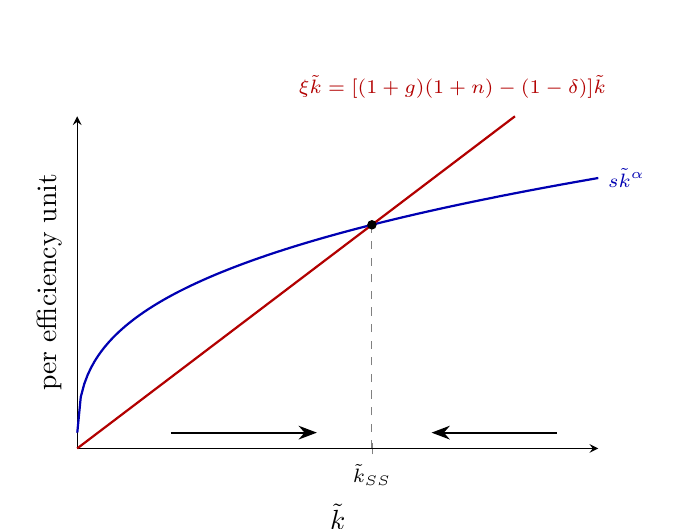
\begin{tikzpicture}
\begin{axis}[width=8.2cm,height=5.8cm,axis lines=left,xmin=0,xmax=5,ymin=0,ymax=0.42,clip=false,
  xlabel={$\tilde k$},ylabel={per efficiency unit},xtick={2.828},xticklabels={$\tilde k_{SS}$},ytick=\empty,
  every tick label/.append style={font=\scriptsize}]
\addplot[domain=0.001:5,samples=150,thick,blue!70!black]{0.2*x^(1/3)};
\addplot[domain=0:4.2,thick,red!70!black]{0.1*x};
\node[font=\scriptsize,blue!70!black,anchor=west] at (axis cs:5,0.342){$s\tilde k^{\alpha}$};
\node[font=\scriptsize,red!70!black,anchor=south] at (axis cs:3.6,0.43){$\xi\tilde k=[(1+g)(1+n)-(1-\delta)]\tilde k$};
\draw[dashed,gray](axis cs:2.828,0)--(axis cs:2.828,0.2828);
\addplot[only marks,mark=*,mark size=1.5pt]coordinates{(2.828,0.2828)};
\draw[-{Stealth},thick](axis cs:0.9,0.02)--(axis cs:2.3,0.02);
\draw[-{Stealth},thick](axis cs:4.6,0.02)--(axis cs:3.4,0.02);
\end{axis}
\end{tikzpicture}\\
{\footnotesize Figure 1. Steady state per efficiency unit. Left of $\tilde k_{SS}$ investment exceeds break-even
investment and $\tilde k$ rises; right of it, $\tilde k$ falls. (Drawn for $\alpha=1/3$, $s=0.2$, $\xi=0.1$.)}
\end{center}
\intuicao{Solow with technological progress is the no-progress model with one change of units: count
workers in efficiency units and the economy settles at a constant $\tilde k$; in per-worker units that same
point is a path growing at $g$.}
\refbib{Kurlat \S4.2, pp.~57--61 (law of motion, steady state, stability); \S4.5, pp.~69--72 (efficiency units,
balanced growth path).}
\rubrica{
\item Stationary variables defined and $\tilde y=\tilde k^{\alpha}$: 0.2 pt.
\item Ratio $\tilde k_{t+1}/\tilde k_t$ with $(1+g)(1+n)$ in the denominator: 0.3 pt.
\item $\tilde k_{SS}$: 0.2 pt. Diagram (axes, both curves named, $\tilde k_{SS}$ marked): 0.1 pt.
\item Growth rates of $y$ and $Y$ with the reason: 0.2 pt.
\item Dividing (2) by $A_tL_t$ instead of $A_{t+1}L_{t+1}$ (no $(1+g)(1+n)$): max.\ 0.5 pt. Working with $K/L$ as if stationary: max.\ 0.4 pt.
}
\end{sol}

\sub{2.b}{1 point} Show which saving rate maximises steady-state consumption per efficiency unit
of labour (the golden-rule rate, $s_{GR}$). Explain why the same $s_{GR}$ also maximises consumption
per worker at every date along the steady state, and how a faster rate of technological progress
$g$ changes $s_{GR}$ and $\tilde k_{GR}$. Give the economic intuition.
\resolespaco[7cm]
\begin{sol}
\begin{notacao}
\item As in 2.a. New: $\tilde c_{SS}(s)$, steady-state consumption per efficiency unit as a function
of the saving rate.
\item $f(\tilde k)\equiv\tilde k^{\alpha}$: output per efficiency unit, by \eqref{q2a:y}.
\item $s_{GR}\in(0,1)$, $\tilde k_{GR}>0$: golden-rule saving rate and capital per efficiency unit.
\item $c_t\equiv C_t/L_t$: consumption per worker. $A_0>0$: technology at date 0.
\end{notacao}
\passo{consumption in steady state}{Consumption is the part of output not saved:}
\begin{equation}
\tilde c_t=(1-s)\,\tilde y_t. \label{q2b:c}
\end{equation}
Substitute \eqref{q2a:yss} into \eqref{q2b:c}, carrying the exponent $\alpha$ of
$\tilde k_{SS}^{\alpha}$ through the substitution:
\begin{align}
\tilde c_{SS}(s) &= (1-s)\,\tilde k_{SS}^{\alpha}\nonumber\\
&= (1-s)\left[\left(\frac{s}{\xi}\right)^{\frac{1}{1-\alpha}}\right]^{\alpha}\nonumber\\
&= (1-s)\left(\frac{s}{\xi}\right)^{\frac{\alpha}{1-\alpha}}. \label{q2b:css}
\end{align}
\passo{first-order condition}{Take the log of \eqref{q2b:css}:}
\begin{equation}
\ln\tilde c_{SS}=\ln(1-s)+\frac{\alpha}{1-\alpha}\ln s-\frac{\alpha}{1-\alpha}\ln\xi. \label{q2b:log}
\end{equation}
Differentiate \eqref{q2b:log} with respect to $s$ and set it to zero:
\begin{equation}
\frac{d\ln\tilde c_{SS}}{ds}=-\frac{1}{1-s}+\frac{\alpha}{(1-\alpha)s}=0. \label{q2b:foc}
\end{equation}
Multiply \eqref{q2b:foc} by $(1-\alpha)s(1-s)>0$:
\begin{align*}
-(1-\alpha)s+\alpha(1-s) &= 0\\
\alpha(1-s) &= (1-\alpha)s\\
\alpha-\alpha s &= s-\alpha s\\
\alpha &= s.
\end{align*}
Hence
\begin{equation}
\boxed{s_{GR}=\alpha} \label{q2b:sgr}
\end{equation}
SOC: differentiate \eqref{q2b:foc} once more:
\[
\frac{d^2\ln\tilde c_{SS}}{ds^2}=-\frac{1}{(1-s)^2}-\frac{\alpha}{(1-\alpha)s^2}<0,
\]
so \eqref{q2b:sgr} is a maximum.
\passo{cross-check by $\tilde k$}{Substitute \eqref{q2a:y} into \eqref{q2b:c}, then use the
steady-state condition \eqref{q2a:break}, $s\tilde k^{\alpha}=\xi\tilde k$:}
\begin{align}
\tilde c &= (1-s)\big(\tilde k^{\alpha}\big)\nonumber\\
&= \tilde k^{\alpha}-s\tilde k^{\alpha}\nonumber\\
&= \tilde k^{\alpha}-\big(\xi\tilde k\big). \label{q2b:ck}
\end{align}
Maximise \eqref{q2b:ck} over $\tilde k$:
\begin{equation}
\boxed{f'(\tilde k_{GR})=\alpha\tilde k_{GR}^{\alpha-1}=\xi=(1+g)(1+n)-(1-\delta)} \label{q2b:mpk}
\end{equation}
The marginal product of capital equals break-even investment per unit of capital. Solve
\eqref{q2b:mpk} for $\tilde k_{GR}$:
\begin{equation}
\tilde k_{GR}^{1-\alpha}=\frac{\alpha}{\xi}. \label{q2b:kgr}
\end{equation}
Solve \eqref{q2a:break} for $s$ at $\tilde k_{GR}$ and use \eqref{q2b:kgr} in the third line:
\begin{align*}
s &= \frac{\xi\tilde k_{GR}}{\tilde k_{GR}^{\alpha}}\\
&= \xi\,\tilde k_{GR}^{1-\alpha}\\
&= \xi\cdot\frac{\alpha}{\xi}\\
&= \alpha\ \checkmark
\end{align*}
\passo{per worker, every date}{Invert \eqref{q2a:def} and use \eqref{q2:A}:}
\begin{align}
c_t &= \frac{C_t}{L_t}=A_t\,\tilde c_{SS}\nonumber\\
&= A_0(1+g)^t\,\tilde c_{SS}. \label{q2b:cpw}
\end{align}
Take logs of \eqref{q2b:cpw}:
\begin{equation}
\ln c_t=\ln A_0+t\ln(1+g)+\ln\tilde c_{SS}(s). \label{q2b:lncpw}
\end{equation}
$A_t$ does not depend on $s$, so the $s$ that maximises $\tilde c_{SS}$ raises the whole path
\eqref{q2b:lncpw} by the same amount at every $t$: the golden rule maximises consumption per worker
at \emph{every} date of the steady state.
\passo{effect of $g$}{$g$ does not appear in \eqref{q2b:sgr}: $s_{GR}=\alpha$ is
\textbf{unchanged}. Solving \eqref{q2b:kgr},}
\[
\tilde k_{GR}=\left(\frac{\alpha}{\xi}\right)^{\frac{1}{1-\alpha}},
\]
and by \eqref{q2a:xi}, $\partial\xi/\partial g=1+n>0$, so $\boxed{\tilde k_{GR}\downarrow}$. Faster
progress makes keeping $\tilde k$ constant more expensive (steeper break-even line), so the
consumption-maximising capital per efficiency unit is lower; but the \emph{share} of output to save
does not move, because with Cobb--Douglas the capital income $\alpha\tilde y$ always equals the
break-even investment $\xi\tilde k$ exactly at the golden rule.
\passo{knife-edge check}{$\alpha\to0$: capital is useless and $s_{GR}\to0$ in \eqref{q2b:sgr}.
Dropping the exponent (using $(s/\xi)^{1/(1-\alpha)}$ for $\tilde y$ in \eqref{q2b:css}) gives
$s=1/(2-\alpha)\to1/2$, which fails this test.}
\begin{center}
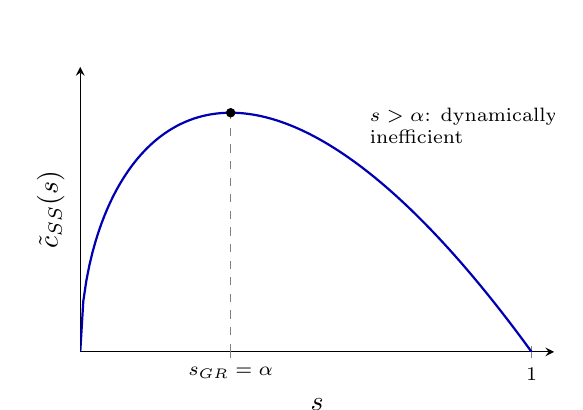
\begin{tikzpicture}
\begin{axis}[width=7.6cm,height=5.2cm,axis lines=left,xmin=0,xmax=1.05,ymin=0,ymax=1.45,
  xlabel={$s$},ylabel={$\tilde c_{SS}(s)$},xtick={0.3333,1},xticklabels={$s_{GR}=\alpha$,$1$},ytick=\empty,
  every tick label/.append style={font=\scriptsize}]
\addplot[domain=0:1,samples=150,thick,blue!70!black]{(1-x)*sqrt(x/0.1)};
\draw[dashed,gray](axis cs:0.3333,0)--(axis cs:0.3333,1.217);
\addplot[only marks,mark=*,mark size=1.5pt]coordinates{(0.3333,1.217)};
\node[font=\scriptsize,anchor=west,align=left] at (axis cs:0.62,1.15){$s>\alpha$: dynamically\\inefficient};
\end{axis}
\end{tikzpicture}\\
{\footnotesize Figure 2. Steady-state consumption per efficiency unit against $s$ (drawn for $\alpha=1/3$, $\xi=0.1$):
zero at $s=0$ (nothing to consume from) and at $s=1$ (nothing consumed), maximum at $s=\alpha$.}
\end{center}
\intuicao{Saving more raises $\tilde k$ and output, but each extra unit of capital also needs $\xi$ of
investment every period just to be kept per efficiency unit. Consumption is maximised when the last unit
of capital produces exactly what it costs to maintain: $f'(\tilde k)=\xi$. Above that point ($s>\alpha$) the
economy could consume more today and forever by saving less.}
\refbib{Kurlat \S4.3, pp.~61--63 (golden rule, $s_{gold}=\alpha$); \S4.5, pp.~69--72.}
\rubrica{
\item $\tilde c_{SS}(s)$ with exponent $\alpha/(1-\alpha)$: 0.3 pt.
\item FOC and $s_{GR}=\alpha$ (SOC or cross-check $f'=\xi$): 0.3 pt.
\item Per-worker consumption at every date maximised: 0.2 pt. Effect of $g$ on $s_{GR}$ and $\tilde k_{GR}$: 0.1 pt.
\item Intuition (marginal product equals break-even cost): 0.1 pt.
\item Exponent dropped in the substitution ($s=1/(2-\alpha)$): max.\ 0.4 pt. Maximising $\tilde k$ (answer $s=1$): max.\ 0.2 pt.
}
\gap{Prova 01, 2.b: the $\sigma$ (here $\alpha$) in the exponent of $c_{SS}$ was dropped.}
\end{sol}

\sub{2.c}{1 point} Consider now the competitive equilibrium of an economy that lasts only two
periods, $t=1,2$. There is an initial capital stock $K_1>0$, which belongs to the representative
firm and depreciates fully once used in period~1. The representative firm maximises profits in
perfectly competitive markets and has production function (1) in both periods, with
$A_2=(1+g)A_1$. The representative consumer owns the firm and receives its profits $\Pi_1$ and
$\Pi_2$. In each period the consumer has one unit of time, which it splits between work $L_t$ and
leisure $1-L_t$, and earns real labour income $w_tA_tL_t$ ($w_t$ is the real wage per efficiency
unit of labour). Income not consumed in period~1 is saved as an asset $a_1$ that pays the real
interest rate $r$; the only asset in this economy is the capital the firm uses in period~2, $K_2$,
which also depreciates fully once used. Intertemporal utility is
\[
U=\ln c_1+\gamma\ln(1-L_1)+\beta\left[\ln c_2+\gamma\ln(1-L_2)\right],\qquad \beta\in(0,1),\ \gamma>0.
\]
Derive and explain the intertemporal budget constraint of this consumer.
\resolespaco[6cm]
\begin{sol}
\begin{notacao}
\item $c_1$, $c_2>0$: consumption in periods 1 and 2. $L_t\in[0,1]$: hours worked; $1-L_t$: leisure
(time endowment normalised to 1).
\item $A_t>0$: technology, with $A_2=(1+g)A_1$. $w_t>0$: real wage per efficiency unit of labour, so
labour income is $w_tA_tL_t$.
\item $\Pi_1$, $\Pi_2$: the firm's profits, paid to the consumer who owns it.
\item $a_1$: asset carried from period 1 to period 2; of either sign for one consumer (in
equilibrium it is the capital $K_2>0$). $r>-1$: real interest rate between the periods.
\item $\beta\in(0,1)$: discount factor. $\gamma>0$: weight of leisure in utility.
\item $H>0$: full lifetime income, the present value of the time endowment plus profits (step 3).
\end{notacao}
\passo{period constraints}{In period 1, uses equal sources:}
\begin{equation}
\boxed{c_1+a_1=w_1A_1L_1+\Pi_1} \label{q2c:b1}
\end{equation}
Period 2 is the last: nothing is left for later, and nobody would lend to a consumer who cannot
repay after period 2. So the consumer spends the asset with its return plus period-2 income:
\begin{equation}
\boxed{c_2=(1+r)a_1+w_2A_2L_2+\Pi_2} \label{q2c:b2}
\end{equation}
Profits appear because the consumer owns the firm; with no initial financial wealth, they are its
only non-labour income besides the return on $a_1$.
\passo{eliminate $a_1$}{Solve \eqref{q2c:b2} for $a_1$:}
\begin{equation}
a_1=\frac{c_2-w_2A_2L_2-\Pi_2}{1+r}. \label{q2c:a1}
\end{equation}
Substitute \eqref{q2c:a1} into \eqref{q2c:b1}:
\[
c_1+\frac{c_2-w_2A_2L_2-\Pi_2}{1+r}=w_1A_1L_1+\Pi_1 .
\]
Move the period-2 income terms to the right side:
\begin{equation}
\boxed{c_1+\frac{c_2}{1+r}=w_1A_1L_1+\Pi_1+\frac{w_2A_2L_2+\Pi_2}{1+r}} \label{q2c:ibc}
\end{equation}
\passo{full-income form}{Value leisure at its opportunity cost, the wage. Add
$w_1A_1(1-L_1)+\frac{w_2A_2(1-L_2)}{1+r}$ to both sides of \eqref{q2c:ibc}; on the right,
$w_tA_tL_t+w_tA_t(1-L_t)=w_tA_t$:}
\begin{align}
&c_1+w_1A_1(1-L_1)+\frac{c_2+w_2A_2(1-L_2)}{1+r}\nonumber\\
&\qquad=\big[w_1A_1L_1+w_1A_1(1-L_1)\big]+\Pi_1+\frac{\big[w_2A_2L_2+w_2A_2(1-L_2)\big]+\Pi_2}{1+r}\nonumber\\
&\qquad=H, \label{q2c:full}
\end{align}
where
\begin{equation}
H\equiv w_1A_1+\Pi_1+\frac{w_2A_2+\Pi_2}{1+r}. \label{q2c:H}
\end{equation}
\passo{reading}{By \eqref{q2c:full}--\eqref{q2c:H}, the \textbf{present value} of lifetime
consumption (and of leisure, priced at the wage) equals the present value of lifetime income: the
value of the whole time endowment plus profits, with period-2 amounts discounted at $1+r$. $a_1$ may
be of either sign for one consumer; it disappears from the lifetime constraint \eqref{q2c:ibc}
because borrowing and lending only move resources across periods at the price $1/(1+r)$. The
constraint binds: $u'>0$, so unspent resources at the end are never optimal.}
\refbib{Kurlat \S6.2, pp.~105--112 (intertemporal budget constraint); \S7.2, pp.~131--137 (time endowment,
labour income); ch.~9, \S9.1 (households own the firms).}
\rubrica{
\item Two period constraints, with $\Pi_1,\Pi_2$ and the labour income of both periods: 0.4 pt.
\item Elimination of $a_1$ to the present-value constraint: 0.3 pt.
\item Explanation as a present-value statement (why $1+r$ discounts, why it binds): 0.3 pt.
\item Profits omitted: $-0.2$. ``Consumption adjusted by $r$'' without the present-value reading: max.\ 0.1 on the last line.
}
\gap{Prova 01, 2.c: firm profits omitted from the budget constraint; reading not stated in present value.}
\end{sol}

\sub{2.d}{1 point} Set up the problem of the consumer of item 2.c and derive the first-order
conditions for \emph{all} of its choice variables, including the equation describing the
intertemporal consumption decision and the consumption--leisure decision in each period. Then find
the equation that gives the optimal $c_1$ as a function only of parameters, prices and levels of
income and wealth, and interpret it economically.
\resolespaco[7cm]
\begin{sol}
\begin{notacao}
\item As in 2.c. New: $\lambda_1$, $\lambda_2>0$, the multipliers on \eqref{q2c:b1} and
\eqref{q2c:b2}: the marginal utility of one more unit of income in period $t$.
\end{notacao}
\passo{problem}{Choice variables: $c_1,c_2,L_1,L_2,a_1$; prices $w_1,w_2,r$ and profits
$\Pi_1,\Pi_2$ are taken as given. Maximise $U$ subject to \eqref{q2c:b1} and \eqref{q2c:b2}, with
one multiplier per period constraint:}
\begin{align}
\mathcal L={}&\ln c_1+\gamma\ln(1-L_1)+\beta\ln c_2+\beta\gamma\ln(1-L_2)\nonumber\\
&+\lambda_1\left[w_1A_1L_1+\Pi_1-c_1-a_1\right]+\lambda_2\left[(1+r)a_1+w_2A_2L_2+\Pi_2-c_2\right]. \label{q2d:lag}
\end{align}
\passo{FOCs}{Differentiate \eqref{q2d:lag} with respect to each choice variable and set the
derivative to zero:}
\begin{align}
c_1:&\quad \frac{1}{c_1}=\lambda_1, \label{q2d:c1}\\
c_2:&\quad \frac{\beta}{c_2}=\lambda_2, \label{q2d:c2}\\
L_1:&\quad \frac{\gamma}{1-L_1}=\lambda_1w_1A_1, \label{q2d:L1}\\
L_2:&\quad \frac{\beta\gamma}{1-L_2}=\lambda_2w_2A_2, \label{q2d:L2}\\
a_1:&\quad \lambda_1=(1+r)\lambda_2. \label{q2d:a1}
\end{align}
Log utility makes every solution interior: as $L_t\to1$ the marginal utility of leisure goes to
infinity, and as $c_t\to0$ that of consumption does.
\passo{Euler (intertemporal)}{Substitute \eqref{q2d:c1} and \eqref{q2d:c2} into \eqref{q2d:a1}:}
\begin{align*}
\left(\frac{1}{c_1}\right) &= (1+r)\left(\frac{\beta}{c_2}\right)\\
\frac{1}{c_1} &= \beta(1+r)\frac{1}{c_2}.
\end{align*}
Multiply by $c_1c_2$:
\begin{equation}
\boxed{c_2=\beta(1+r)\,c_1} \label{q2d:euler}
\end{equation}
The marginal rate of substitution between $c_1$ and $c_2$ equals the relative price $1+r$.
\passo{consumption--leisure (intratemporal)}{Divide \eqref{q2d:L1} by \eqref{q2d:c1}, and
\eqref{q2d:L2} by \eqref{q2d:c2}; the multipliers cancel:}
\begin{align*}
\frac{\gamma/(1-L_1)}{1/c_1} &= \frac{\lambda_1w_1A_1}{\lambda_1},\\
\frac{\beta\gamma/(1-L_2)}{\beta/c_2} &= \frac{\lambda_2w_2A_2}{\lambda_2}.
\end{align*}
\begin{equation}
\boxed{\frac{\gamma c_1}{1-L_1}=w_1A_1} \label{q2d:intra1}
\end{equation}
\begin{equation}
\boxed{\frac{\gamma c_2}{1-L_2}=w_2A_2} \label{q2d:intra2}
\end{equation}
In each period the MRS between leisure and consumption equals the real wage (the price of an hour
of leisure).
\passo{solve for $c_1$}{Express each term on the left of the full-income constraint
\eqref{q2c:full} in terms of $c_1$. From \eqref{q2d:euler}, \eqref{q2d:intra1}, and
\eqref{q2d:intra2} followed by \eqref{q2d:euler}:}
\begin{align}
\frac{c_2}{1+r} &= \frac{\big[\beta(1+r)c_1\big]}{1+r}\nonumber\\
&= \beta c_1, \label{q2d:t1}\\
w_1A_1(1-L_1) &= \gamma c_1, \label{q2d:t2}\\
\frac{w_2A_2(1-L_2)}{1+r} &= \frac{\gamma c_2}{1+r}\nonumber\\
&= \frac{\gamma\big[\beta(1+r)c_1\big]}{1+r}\nonumber\\
&= \beta\gamma c_1. \label{q2d:t3}
\end{align}
Split the fraction in \eqref{q2c:full} and substitute \eqref{q2d:t1}--\eqref{q2d:t3}:
\begin{align*}
c_1+w_1A_1(1-L_1)+\frac{c_2}{1+r}+\frac{w_2A_2(1-L_2)}{1+r} &= H\\
c_1+(\gamma c_1)+(\beta c_1)+(\beta\gamma c_1) &= H\\
c_1(1+\gamma+\beta+\beta\gamma) &= H\\
c_1(1+\beta)(1+\gamma) &= H.
\end{align*}
Divide by $(1+\beta)(1+\gamma)$ and write $H$ out with \eqref{q2c:H}:
\begin{align}
c_1 &= \frac{H}{(1+\beta)(1+\gamma)}\nonumber\\
&= \boxed{\frac{1}{(1+\beta)(1+\gamma)}\left[w_1A_1+\Pi_1+\frac{w_2A_2+\Pi_2}{1+r}\right]} \label{q2d:c1sol}
\end{align}
Then \eqref{q2d:euler}, \eqref{q2d:intra1}--\eqref{q2d:intra2} and \eqref{q2c:b1} give the other
choices:
\begin{align*}
c_2 &= \beta(1+r)\,c_1,\\
1-L_t &= \frac{\gamma c_t}{w_tA_t},\quad t=1,2,\\
a_1 &= w_1A_1L_1+\Pi_1-c_1.
\end{align*}
\passo{interpretation}{By \eqref{q2d:t1}--\eqref{q2d:c1sol}, with log utility the consumer spends fixed shares of full lifetime wealth $H$:
$\frac{1}{(1+\beta)(1+\gamma)}$ on $c_1$, $\frac{\gamma}{(1+\beta)(1+\gamma)}$ on leisure in period 1,
$\frac{\beta}{(1+\beta)(1+\gamma)}$ and $\frac{\beta\gamma}{(1+\beta)(1+\gamma)}$ on period~2.
$c_1$ depends on \emph{lifetime} resources, not on period-1 income alone (permanent income).
$\beta\uparrow\Rightarrow c_1\downarrow$ (patience moves spending to period 2); $\gamma\uparrow\Rightarrow
c_1\downarrow$ for given $H$ (more of full wealth is taken as leisure). Given $H$, $r$ does not enter: for
the shares, the income and substitution effects of $r$ cancel with log utility; $r$ moves $c_1$ only
through the present value of period-2 income in $H$ (a higher $r$ lowers it, so $c_1$ falls).}
\intuicao{Contrast with Prova 01: there work had no utility cost, so $L_1=1$ was a corner and saying so
was the FOC. Here leisure is valued, so hours are an interior choice and the wage is the price of leisure.}
\refbib{Kurlat \S6.2, pp.~105--115 (Euler equation, log closed forms); \S7.2, pp.~131--137 (consumption--leisure);
ch.~9, \S9.1, eq.~(9.1.7)--(9.1.8).}
\rubrica{
\item Problem stated with all five choice variables: 0.1 pt.
\item FOCs for $c_1,c_2$ and the Euler equation: 0.3 pt. FOCs for $L_1$ and $L_2$ (intratemporal conditions): 0.2 pt (0.1 each).
\item FOC for $a_1$ (or the substitution that eliminates it): 0.1 pt.
\item $c_1$ in closed form: 0.2 pt. Interpretation ($H$, $\beta$, $\gamma$, role of $r$): 0.1 pt.
\item No FOC for hours: max.\ 0.6 pt. Substitution route instead of Lagrangian: full credit.
}
\gap{Prova 01, 2.d: FOC for $L_1$ missing (``todas as variáveis de sua escolha'').}
\end{sol}

\sub{2.e}{1 point} Calculate the saving rate of this representative consumer (the share of saving
in the consumer's period-1 income), recalling that markets are perfectly competitive. Find the hours
worked in each period. Then find an expression for $\hat k_2\equiv K_2/A_2$ as a function only of
$\hat k_1\equiv K_1/A_1$ and of parameters. Treating this expression as a law of motion that applies
period after period, draw it with $\hat k_1$ on the horizontal axis and $\hat k_2$ on the vertical
axis, and show graphically the steady state of this economy. Is it stable? Justify.
\resolespaco[8cm]
\begin{sol}
\begin{notacao}
\item As in 2.c--2.d. New: $Y_1$, $Y_2>0$, output in each period by \eqref{q2:Y}; $K_2>0$, the
capital built from period-1 saving.
\item $s^\ast\in(0,1)$: the consumer's saving rate. $\hat k_t\equiv K_t/A_t>0$: capital per unit of
technology.
\item $\phi(\hat k)$: the law of motion $\hat k_{t+1}=\phi(\hat k_t)$. $\hat k_{SS}$: its fixed point.
$\hat k_{GR}$ (Figure 3): the fixed point of the same map with $s=s_{GR}$.
\end{notacao}
\passo{firm, period 1}{The firm owns $K_1$ and hires labour:}
\begin{equation}
\max_{L_1}\ K_1^{\alpha}(A_1L_1)^{1-\alpha}-w_1A_1L_1. \label{q2e:firm1}
\end{equation}
The FOC of \eqref{q2e:firm1}, with $Y_1$ from \eqref{q2:Y}:
\begin{equation}
(1-\alpha)\frac{Y_1}{L_1}=w_1A_1. \label{q2e:foc1}
\end{equation}
Multiply \eqref{q2e:foc1} by $L_1$ to get the wage bill:
\begin{equation}
w_1A_1L_1=(1-\alpha)Y_1. \label{q2e:wb1}
\end{equation}
Profit is output minus the wage bill \eqref{q2e:wb1}:
\begin{align}
\Pi_1 &= Y_1-w_1A_1L_1\nonumber\\
&= Y_1-(1-\alpha)Y_1\nonumber\\
&= \boxed{\alpha Y_1}, \label{q2e:pi1}
\end{align}
the return on the capital the firm owns, paid to its owner.
\passo{firm, period 2}{The firm borrows $K_2$ from the consumer and repays $(1+r)K_2$ (the capital
is used up):}
\begin{equation}
\max_{K_2,L_2}\ K_2^{\alpha}(A_2L_2)^{1-\alpha}-w_2A_2L_2-(1+r)K_2. \label{q2e:firm2}
\end{equation}
The FOCs of \eqref{q2e:firm2}:
\begin{align}
\alpha\frac{Y_2}{K_2} &= 1+r, \label{q2e:r}\\
(1-\alpha)\frac{Y_2}{L_2} &= w_2A_2. \label{q2e:w2}
\end{align}
Multiply \eqref{q2e:r} by $K_2$ and \eqref{q2e:w2} by $L_2$ and subtract both payments from output.
With constant returns:
\begin{align}
\Pi_2 &= Y_2-w_2A_2L_2-(1+r)K_2\nonumber\\
&= Y_2-(1-\alpha)Y_2-\alpha Y_2\nonumber\\
&= \boxed{0}. \label{q2e:pi2}
\end{align}
\passo{market clearing}{The only asset is the capital of period 2, so the asset market clears when}
\begin{equation}
\boxed{a_1=K_2} \label{q2e:mc}
\end{equation}
The goods markets clear when
\begin{align}
c_1+K_2 &= Y_1, \label{q2e:g1}\\
c_2 &= Y_2. \label{q2e:g2}
\end{align}
Labour: $L_t$ supplied $=$ $L_t$ demanded. Check: by \eqref{q2e:r}, \eqref{q2e:w2} and
\eqref{q2e:pi2}, period-2 income in \eqref{q2c:b2} is
\[
(1+r)K_2+w_2A_2L_2+\Pi_2=\alpha Y_2+(1-\alpha)Y_2+0=Y_2 .
\]
\passo{saving rate}{Substitute \eqref{q2e:g2} and \eqref{q2e:r} into the Euler equation
\eqref{q2d:euler}, then multiply by $K_2/Y_2$:}
\begin{align}
(Y_2) &= \beta\left(\frac{\alpha Y_2}{K_2}\right)c_1\nonumber\\
K_2 &= \alpha\beta\,c_1. \label{q2e:K2c1}
\end{align}
Substitute \eqref{q2e:K2c1} into the period-1 goods market \eqref{q2e:g1}:
\begin{align}
c_1+(\alpha\beta c_1) &= Y_1\nonumber\\
c_1 &= \frac{Y_1}{1+\alpha\beta}. \label{q2e:c1}
\end{align}
Substitute \eqref{q2e:c1} into \eqref{q2e:K2c1} and use \eqref{q2e:mc}:
\begin{align}
K_2 &= \alpha\beta\left(\frac{Y_1}{1+\alpha\beta}\right)\nonumber\\
a_1=K_2 &= \frac{\alpha\beta}{1+\alpha\beta}\,Y_1. \label{q2e:a1}
\end{align}
Period-1 income, by \eqref{q2e:wb1} and \eqref{q2e:pi1}:
\begin{align}
w_1A_1L_1+\Pi_1 &= (1-\alpha)Y_1+\alpha Y_1\nonumber\\
&= Y_1. \label{q2e:inc1}
\end{align}
Divide \eqref{q2e:a1} by \eqref{q2e:inc1}:
\begin{align}
s^\ast &= \frac{a_1}{w_1A_1L_1+\Pi_1}\nonumber\\
&= \frac{\left(\frac{\alpha\beta}{1+\alpha\beta}\,Y_1\right)}{(Y_1)}\nonumber\\
&= \boxed{\frac{\alpha\beta}{1+\alpha\beta}}\quad\text{(constant: no }K_1,A_1,g,\gamma\text{)}. \label{q2e:s}
\end{align}
\passo{hours}{Period 2: substitute \eqref{q2e:g2} for $c_2$ and \eqref{q2e:w2} for $w_2A_2$ into
\eqref{q2d:intra2}:}
\begin{align}
\frac{\gamma(Y_2)}{1-L_2} &= \left(\frac{(1-\alpha)Y_2}{L_2}\right)\nonumber\\
\gamma L_2 &= (1-\alpha)(1-L_2)\nonumber\\
L_2(1-\alpha+\gamma) &= 1-\alpha\nonumber\\
L_2 &= \boxed{\frac{1-\alpha}{1-\alpha+\gamma}}. \label{q2e:L2}
\end{align}
Period 1: substitute \eqref{q2e:c1} for $c_1$ and \eqref{q2e:foc1} for $w_1A_1$ into
\eqref{q2d:intra1}:
\begin{align}
\frac{\gamma\left(\frac{Y_1}{1+\alpha\beta}\right)}{1-L_1} &= \left(\frac{(1-\alpha)Y_1}{L_1}\right)\nonumber\\
\frac{\gamma Y_1}{(1+\alpha\beta)(1-L_1)} &= \frac{(1-\alpha)Y_1}{L_1}\nonumber\\
\gamma L_1 &= (1-\alpha)(1+\alpha\beta)(1-L_1)\nonumber\\
L_1\big[(1-\alpha)(1+\alpha\beta)+\gamma\big] &= (1-\alpha)(1+\alpha\beta)\nonumber\\
L_1 &= \boxed{\frac{(1-\alpha)(1+\alpha\beta)}{(1-\alpha)(1+\alpha\beta)+\gamma}}. \label{q2e:L1}
\end{align}
Neither \eqref{q2e:L2} nor \eqref{q2e:L1} depends on $K_1$ or $A_t$: with log utility the income and
substitution effects of a higher wage cancel. $L_1>L_2$: in period 1 consumption is only the share
$1/(1+\alpha\beta)$ of output, so a unit of income is worth more at the margin (part of it is saved)
and the consumer works more.
\passo{law of motion}{By \eqref{q2e:a1}, \eqref{q2e:s} and \eqref{q2:Y}:}
\begin{align}
K_2 &= s^\ast Y_1\nonumber\\
&= s^\ast K_1^{\alpha}(A_1L_1)^{1-\alpha}. \label{q2e:K2}
\end{align}
Divide \eqref{q2e:K2} by $A_2=(1+g)A_1$ and use $K_1=\hat k_1A_1$:
\begin{align}
\hat k_2 &= \frac{s^\ast(\hat k_1A_1)^{\alpha}(A_1L_1)^{1-\alpha}}{(1+g)A_1}\nonumber\\
&= \frac{s^\ast A_1\,\hat k_1^{\alpha}L_1^{1-\alpha}}{(1+g)A_1}\nonumber\\
&= \boxed{\frac{s^\ast L_1^{1-\alpha}}{1+g}\,\hat k_1^{\alpha}}\equiv\phi(\hat k_1). \label{q2e:phi}
\end{align}
\passo{steady state and stability}{From \eqref{q2e:phi}: $\phi(0)=0$, $\phi'>0$, $\phi''<0$,
$\phi'\to\infty$ as $\hat k\to0$ and $\phi'\to0$ as $\hat k\to\infty$. The curve starts above the
45-degree line and ends below it, so it crosses it exactly once at a positive point. Set
$\hat k=\phi(\hat k)$ in \eqref{q2e:phi}:}
\begin{align*}
\hat k &= \frac{s^\ast L_1^{1-\alpha}}{1+g}\,\hat k^{\alpha}\\
\hat k^{1-\alpha} &= \frac{s^\ast L_1^{1-\alpha}}{1+g}.
\end{align*}
Raise both sides to the power $1/(1-\alpha)$:
\begin{equation}
\boxed{\hat k_{SS}=\left(\frac{s^\ast L_1^{1-\alpha}}{1+g}\right)^{\frac{1}{1-\alpha}}} \label{q2e:kss}
\end{equation}
Differentiate \eqref{q2e:phi}:
\begin{align*}
\phi'(\hat k) &= \alpha\,\frac{s^\ast L_1^{1-\alpha}}{1+g}\,\hat k^{\alpha-1}\\
&= \alpha\,\frac{\phi(\hat k)}{\hat k}.
\end{align*}
At the fixed point $\phi(\hat k_{SS})=\hat k_{SS}$, so
\begin{align*}
\phi'(\hat k_{SS}) &= \alpha\,\frac{\phi(\hat k_{SS})}{\hat k_{SS}}\\
&= \alpha\,\frac{(\hat k_{SS})}{\hat k_{SS}}\\
&= \alpha<1\ \Rightarrow\ \text{stable}.
\end{align*}
From any $\hat k_1<\hat k_{SS}$ the staircase between $\phi$ and the 45-degree line climbs
monotonically to $\hat k_{SS}$ (Figure 3).
\begin{center}
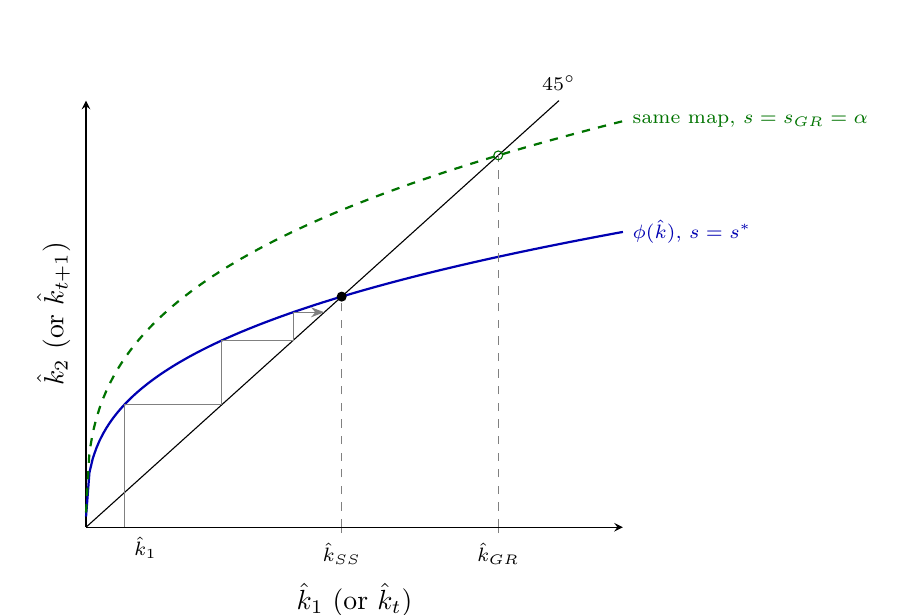
\begin{tikzpicture}
\begin{axis}[width=8.4cm,height=7cm,axis lines=left,xmin=0,xmax=2.1,ymin=0,ymax=1.85,clip=false,
  xlabel={$\hat k_1$ (or $\hat k_t$)},ylabel={$\hat k_2$ (or $\hat k_{t+1}$)},xtick={1,1.6124},
  xticklabels={$\hat k_{SS}$,$\hat k_{GR}$},ytick=\empty,every tick label/.append style={font=\scriptsize}]
\addplot[domain=0:1.85,thin,black]{x};
\addplot[domain=0.0001:2.1,samples=160,thick,blue!70!black]{x^(1/3)};
\addplot[domain=0.0001:2.1,samples=160,thick,dashed,green!45!black]{1.375*x^(1/3)};
\node[font=\scriptsize,anchor=south] at (axis cs:1.85,1.85){$45^\circ$};
\node[font=\scriptsize,blue!70!black,anchor=west] at (axis cs:2.1,1.281){$\phi(\hat k)$, $s=s^\ast$};
\node[font=\scriptsize,green!45!black,anchor=west] at (axis cs:2.1,1.761){same map, $s=s_{GR}=\alpha$};
\draw[gray,-{Stealth}](axis cs:0.15,0)--(axis cs:0.15,0.5313)--(axis cs:0.5313,0.5313)--(axis cs:0.5313,0.8099)
  --(axis cs:0.8099,0.8099)--(axis cs:0.8099,0.9321)--(axis cs:0.9321,0.9321);
\addplot[only marks,mark=*,mark size=1.6pt]coordinates{(1,1)};
\addplot[only marks,mark=o,mark size=1.6pt,green!45!black]coordinates{(1.6124,1.6124)};
\draw[dashed,gray](axis cs:1,0)--(axis cs:1,1);
\draw[dashed,gray](axis cs:1.6124,0)--(axis cs:1.6124,1.6124);
\node[font=\scriptsize,anchor=north west] at (axis cs:0.15,0){$\hat k_1$};
\end{axis}
\end{tikzpicture}\\
{\footnotesize Figure 3. The equilibrium law of motion (solid) crosses the 45-degree line once; the staircase
from a low $\hat k_1$ converges to $\hat k_{SS}$. Dashed: the same map with $s=\alpha$, whose fixed point is the
golden rule (used in 2.f). Drawn for $\alpha=1/3$, $\beta=0.96$, units chosen so that $\hat k_{SS}=1$.}
\end{center}
\intuicao{Patience and the productivity of capital set the saving rate; diminishing returns ($\alpha<1$) make
each extra unit of capital produce less, so saving a fixed share of a concave output cannot sustain unbounded
growth of $\hat k$.}
\refbib{Kurlat ch.~9, \S9.1 (firm FOCs, market clearing, $r=r^K-\delta$ with $\delta=1$); \S4.4, pp.~63--69
(factor shares, zero profit under constant returns); \S4.2, pp.~59--61 (stability).}
\rubrica{
\item Firm FOCs, $\Pi_1=\alpha Y_1$, $\Pi_2=0$, $1+r=\alpha Y_2/K_2$: 0.2 pt.
\item Market clearing $a_1=K_2$ (and goods): 0.1 pt. Saving rate $\alpha\beta/(1+\alpha\beta)$ derived: 0.2 pt.
\item Hours $L_1$, $L_2$: 0.1 pt. Map $\hat k_2(\hat k_1)$: 0.2 pt.
\item Diagram: axes, 45-degree line, concave map from the origin, $\hat k_{SS}$ at the crossing, stability argued: 0.2 pt.
\item Saving rate quoted from Solow's $s$ or left as a function of prices: 0 for that line. No market clearing ($K_2\neq a_1$): max.\ 0.5 pt. A map that does not cross the 45-degree line: 0 for the diagram.
}
\gap{Prova 01, 2.e: saving rate not derived; no market clearing $K_2=a_1$; diagram without a valid steady state.}
\end{sol}

\sub{2.f}{0.5 point} Discuss intuitively the relation between the model of items 2.c--2.e and the
Solow model of items 2.a--2.b. In particular, compare the saving rate found in 2.e with $s_{GR}$ and
explain the difference.
\resolespaco[5cm]
\begin{sol}
\begin{notacao}
\item As in 2.a--2.e. New: $\tilde k_t\equiv\hat k_t/L_1=K_t/(A_tL_1)>0$, capital per efficiency unit
of \emph{hours} (in 2.a, per efficiency unit of workers).
\end{notacao}
\passo{same law of motion}{Write \eqref{q2e:phi}, applied period after period, in terms of
$\tilde k_t=\hat k_t/L_1$:}
\begin{align}
L_1\tilde k_{t+1} &= \frac{s^\ast L_1^{1-\alpha}}{1+g}\,(L_1\tilde k_t)^{\alpha}\nonumber\\
&= \frac{s^\ast L_1}{1+g}\,\tilde k_t^{\alpha}\nonumber\\
(1+g)\tilde k_{t+1} &= s^\ast\tilde k_t^{\alpha}. \label{q2f:lom}
\end{align}
Set $\boxed{\delta=1}$ (capital used up in one period) and $\boxed{n=0}$ (one consumer) in the
Solow law of motion \eqref{q2a:lom}, which is equation \eqref{q2:K} divided as in 2.a:
\begin{align}
\tilde k_{t+1} &= \frac{(1-1)\tilde k_t+s\tilde k_t^{\alpha}}{(1+g)(1+0)}\nonumber\\
&= \frac{s\tilde k_t^{\alpha}}{1+g}\nonumber\\
(1+g)\tilde k_{t+1} &= s\,\tilde k_t^{\alpha}. \label{q2f:solow}
\end{align}
\eqref{q2f:lom} is \eqref{q2f:solow} with $s=s^\ast$. Indeed, by \eqref{q2e:kss},
\begin{align*}
\hat k_{SS} &= \left(\frac{s^\ast L_1^{1-\alpha}}{1+g}\right)^{\frac{1}{1-\alpha}}\\
&= L_1\left(\frac{s^\ast}{1+g}\right)^{\frac{1}{1-\alpha}}\\
&= L_1\left(\frac{s^\ast}{(1+g)(1+0)-(1-1)}\right)^{\frac{1}{1-\alpha}},
\end{align*}
which is 2.a's $\tilde k_{SS}$ \eqref{q2a:kss} times the hours worked.
\passo{what is new}{Solow \emph{assumes} $s$ and the labour input. Here both are \emph{chosen}:
$s^\ast=\alpha\beta/(1+\alpha\beta)$ in \eqref{q2e:s} comes from patience $\beta$ and the return to
capital $\alpha$, and log utility makes it constant (independent of $K$, $A$, $g$) --- a
microfoundation for Solow's constant saving rate. Hours $L_1$ in \eqref{q2e:L1} depend on the taste
for leisure $\gamma$ and on $\beta$.}
\passo{against the golden rule}{Compare \eqref{q2e:s} with $s_{GR}=\alpha$ from \eqref{q2b:sgr}:}
\begin{align*}
s^\ast<\alpha &\iff \frac{\alpha\beta}{1+\alpha\beta}<\alpha\\
&\iff \frac{\beta}{1+\alpha\beta}<1\\
&\iff \beta<1+\alpha\beta\\
&\iff \beta(1-\alpha)<1,
\end{align*}
always true, since $\beta<1$ and $1-\alpha<1$. So $\boxed{s^\ast<\alpha}$ and $\hat k_{SS}<\hat k_{GR}$
(Figure 3): the competitive economy accumulates \emph{less} than the golden rule. Even as
$\beta\to1$, $s^\ast\to\alpha/(1+\alpha)<\alpha$: here saving finances one period of consumption
only, since the horizon ends.
\passo{why this is not a failure}{The golden rule maximises steady-state consumption and ignores that
consumption earlier is worth more to an impatient consumer ($\beta<1$) and that reaching more capital costs
consumption on the way. Markets here are complete and competitive, with no externalities: by the first welfare
theorem the equilibrium is Pareto efficient, and it is below the golden rule, i.e.\ dynamically efficient. The
golden rule is a property of steady states, not a welfare criterion.}
\refbib{Kurlat \S4.3, pp.~61--63; ch.~9, \S9.2 (first welfare theorem) and \S9.3 (comparison with the golden rule).}
\rubrica{
\item Same law of motion with $\delta=1$, $n=0$: 0.1 pt.
\item Saving (and hours) chosen, not assumed, and from which primitives: 0.2 pt.
\item $s^\ast<\alpha$ shown, with the reason (impatience; golden rule not a welfare criterion): 0.2 pt.
\item ``It is Solow with $\delta=1$ and $n=0$'' and nothing else: max.\ 0.1 pt.
}
\gap{Prova 01, 2.f: the endogenous saving rate and its comparison with $s_{GR}$ were missing.}
\end{sol}

% =============================================================================
\questao{3}{3}{Consider the simplified New Keynesian model of Benigno (2015), based on the aggregate
demand and supply equations below (barred variables are long-run values, when all firms reset their
prices; the others are short-run values):
\begin{align}
y &= \bar y+(g-\bar g)-\sigma\left[i-(\bar p-p)\right]-\sigma\ln\beta, \tag{AD}\label{q3:AD}\\
p-p^e &= \kappa\,(y-y_n), \tag{AS}\label{q3:AS}
\end{align}
where $p^e$ is the price set by the firms that cannot reset prices and $y_n$ is short-run natural output,
\begin{equation}
y_n=\frac{1+\eta}{\sigma^{-1}+\eta}\,a+\frac{\sigma^{-1}}{\sigma^{-1}+\eta}\,g-\frac{1}{\sigma^{-1}+\eta}\,\mu , \tag{YN}\label{q3:YN}
\end{equation}
$\mu$ being the mark-up; $\bar y$ is given by the same expression evaluated at the long-run values
$\bar a$, $\bar g$, $\bar\mu$; and $y_e=\frac{1+\eta}{\sigma^{-1}+\eta}a+\frac{\sigma^{-1}}{\sigma^{-1}+\eta}g$ is the
efficient level of output. All variables are log deviations from an efficient steady state. Initially
$a=\bar a=g=\bar g=\mu=\bar\mu=0$, $\bar p=p^e$, and the central bank sets $i=\rho\equiv-\ln\beta$, so that
$y=y_n=y_e=\bar y$ and $p=p^e$.}

\sub{3.a}{1 point} News arrives that productivity will be permanently higher in the long run: $\bar a$
rises by $d\bar a>0$, while current productivity $a$ does not change. With $i$ unchanged, represent
graphically, explaining economically why, the initial equilibrium and the shift that defines the new
equilibrium. Compute $dy$ and $dp$. Indicate the gap $y-y_n$ and the gap $y-y_e$ and use both in your
explanation. Is this boom good for welfare today? Justify.
\resolespaco[7cm]
\begin{sol}
\begin{notacao}
\item $y$, $p$: output and price level today; $\bar y$, $\bar p$: their long-run values, when all
firms have reset prices. All are log deviations from the efficient steady state.
\item $p^e$: the price preset by the firms that cannot reset this period.
\item $i$: nominal interest rate, the central bank's instrument. $\beta\in(0,1)$: discount factor;
$\rho\equiv-\ln\beta>0$: the initial (neutral) rate.
\item $a$, $\bar a$: productivity today and in the long run. $g$, $\bar g$: government spending.
$\mu$, $\bar\mu$: the firms' mark-up. All start at 0.
\item $\sigma>0$: intertemporal elasticity of substitution. $\eta>0$: inverse Frisch elasticity of
labour supply. $\kappa>0$: slope of AS.
\item $y_n$: natural output (flexible prices, with the mark-up). $y_e$: efficient output (no mark-up).
\item $\Gamma\equiv\frac{1+\eta}{\sigma^{-1}+\eta}>0$: response of $y_n$, $y_e$ and $\bar y$ to
productivity.
\end{notacao}
\passo{0, the remaining statement equations}{With $\Gamma$ as defined above, the statement gives
long-run output (the expression \eqref{q3:YN} at long-run values) and efficient output:}
\begin{align}
\bar y &= \Gamma\,\bar a+\frac{\sigma^{-1}}{\sigma^{-1}+\eta}\,\bar g-\frac{1}{\sigma^{-1}+\eta}\,\bar\mu, \label{q3:ybar}\\
y_e &= \Gamma\,a+\frac{\sigma^{-1}}{\sigma^{-1}+\eta}\,g. \label{q3:ye}
\end{align}
Substitute $\rho=-\ln\beta$ into \eqref{q3:AD}, then use the initial values $g=\bar g=0$ and
$\bar p=p^e$:
\begin{align}
y &= \bar y+(g-\bar g)-\sigma\left[i-(\bar p-p)\right]-\sigma(-\rho)\nonumber\\
&= \bar y+(g-\bar g)-\sigma(i-\rho)-\sigma(p-\bar p)\nonumber\\
&= \bar y+(0-0)-\sigma(i-\rho)-\sigma\big(p-(p^e)\big)\nonumber\\
&= \bar y-\sigma(i-\rho)-\sigma(p-p^e). \label{q3:ADr}
\end{align}
\passo{which bar moves which curve}{Differentiate \eqref{q3:ybar} with only $\bar a$ moving:}
\begin{equation}
d\bar y=\Gamma\,d\bar a>0. \label{q3a:dybar}
\end{equation}
$\bar y$ is in AD \eqref{q3:ADr}, so \boxed{\text{AD shifts right}} by $\Gamma d\bar a$ at every
$p$ (up by $\Gamma d\bar a/\sigma$). $y_n$ in \eqref{q3:YN} and $y_e$ in \eqref{q3:ye} depend on the
\emph{current} $a$, $g$, $\mu$, none of which moved: \boxed{\text{AS does not move}} (it still passes
through $(y_n,p^e)$), and $y_e=y_n=0$ still.
\passo{why AD moves (Euler)}{Long-run consumption $\bar c=\bar y$ rises: households expect higher permanent
income and, to smooth consumption, want to consume more \emph{today} at the same real rate
$i-(\bar p-p)$. Current demand for goods rises at every price level.}
\passo{new equilibrium}{With $i=\rho$, \eqref{q3:ADr} and \eqref{q3a:dybar} give AD; with $y_n=0$,
\eqref{q3:AS} gives AS:}
\begin{align}
y &= (\Gamma\,d\bar a)-\sigma(\rho-\rho)-\sigma(p-p^e)\nonumber\\
&= \Gamma\,d\bar a-\sigma(p-p^e), \label{q3a:AD}\\
p-p^e &= \kappa\,(y-0)\nonumber\\
&= \kappa\,y. \label{q3a:AS}
\end{align}
Substitute \eqref{q3a:AS} into \eqref{q3a:AD}:
\begin{align*}
y &= \Gamma\,d\bar a-\sigma(\kappa\,y)\\
y(1+\sigma\kappa) &= \Gamma\,d\bar a.
\end{align*}
Divide by $1+\sigma\kappa$ (the initial $y$ is 0, so $y=dy$):
\begin{equation}
\boxed{dy=\frac{\Gamma\,d\bar a}{1+\sigma\kappa}>0} \label{q3a:dy}
\end{equation}
Substitute \eqref{q3a:dy} into \eqref{q3a:AS}:
\begin{align}
dp &= \kappa\,dy\nonumber\\
&= \kappa\left(\frac{\Gamma\,d\bar a}{1+\sigma\kappa}\right)\nonumber\\
&= \boxed{\frac{\kappa\,\Gamma\,d\bar a}{1+\sigma\kappa}>0}. \label{q3a:dp}
\end{align}
\passo{the two gaps}{Since $y_n=y_e=0$, both gaps equal \eqref{q3a:dy}. $y-y_n=dy>0$: output above
natural, which is why prices rise in \eqref{q3a:dp} (AS: flexible-price firms face higher real
marginal cost, because households must be paid a higher real wage to work more). $y-y_e=dy>0$:
output above the efficient level as well.
Chain: $\bar a\uparrow\to\bar y\uparrow\to c\uparrow$ (Euler) $\to$ AD right $\to y>y_n\to$ marginal cost $\uparrow\to$
flexible firms raise $p$ $\to$ real rate $i-(\bar p-p)\uparrow$, which limits the rise in $y$ (movement along AD).
Firms with preset prices keep $p^e$ and produce whatever is demanded.}
\passo{welfare}{\textbf{No.} Today's technology is unchanged, so the efficient output today is unchanged.
The extra output is produced by working beyond the point where the MRS between leisure and consumption equals
today's productivity, and the price surprise $p>p^e$ creates price dispersion across identical firms. Both
terms of the welfare loss are positive: the economy is overheating on a forecast.}
\begin{center}
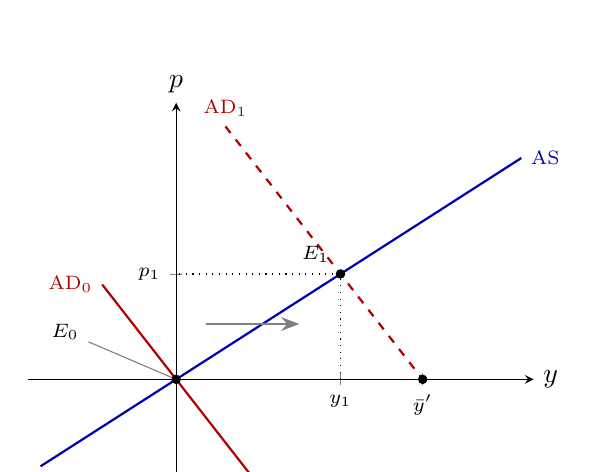
\begin{tikzpicture}
\begin{axis}[width=8cm,height=6.4cm,axis lines=middle,xmin=-0.6,xmax=1.45,ymin=-0.65,ymax=1.75,clip=false,
  xlabel={$y$},ylabel={$p$},xtick={0.6667,1},xticklabels={$y_1$,$\bar y'$},ytick={0.6667},yticklabels={$p_1$},
  every tick label/.append style={font=\scriptsize},x label style={anchor=west},y label style={anchor=south}]
\addplot[thick,blue!70!black,domain=-0.55:1.4]{x};
\addplot[thick,red!70!black,domain=-0.3:0.3]{-2*x};
\addplot[thick,red!70!black,dashed,domain=0.2:1.0]{2-2*x};
\node[font=\scriptsize,blue!70!black,anchor=west] at (axis cs:1.4,1.4){AS};
\node[font=\scriptsize,red!70!black,anchor=east] at (axis cs:-0.3,0.6){AD$_0$};
\node[font=\scriptsize,red!70!black,anchor=south] at (axis cs:0.2,1.6){AD$_1$};
\addplot[only marks,mark=*,mark size=1.5pt]coordinates{(0,0)(0.6667,0.6667)(1,0)};
\node[font=\scriptsize] (e0) at (axis cs:-0.45,0.3){$E_0$};
\draw[gray,thin](e0)--(axis cs:0,0);
\node[font=\scriptsize,anchor=south east] at (axis cs:0.66,0.68){$E_1$};
\draw[dotted](axis cs:0.6667,0)--(axis cs:0.6667,0.6667)--(axis cs:0,0.6667);
\draw[-{Stealth},thick,gray](axis cs:0.12,0.35)--(axis cs:0.5,0.35);
\end{axis}
\end{tikzpicture}\\
{\footnotesize Figure 4. News of higher $\bar a$ shifts AD right (it now passes through $(\bar y',\bar p)$ at $i=\rho$);
AS stays. $E_1$: $y_1-y_n=y_1-y_e>0$ and $p_1>p^e$. (Drawn for $\sigma=0.5$, $\kappa=1$, $\Gamma d\bar a=1$; the origin is
$(y_n,p^e)$.)}
\end{center}
\intuicao{Expectations about the future move demand today. Supply today has not changed, so the extra demand
can only be met by working harder with the same technology, and prices rise.}
\refbib{Benigno (2015) \S6.3, Fig.~8, pp.~511--513; \S5, eqs.~(20)--(21), pp.~509--511; \S4.2--\S4.4 ($y_n$, $y_e$), pp.~508--509.}
\rubrica{
\item AD shifts right, with the Euler/permanent-income reason: 0.3 pt.
\item AS does not move, because $y_n$ depends on current $a,\mu$ only: 0.2 pt.
\item $dy$ and $dp$: 0.2 pt.
\item Both gaps signed and used in the explanation: 0.2 pt. Welfare verdict with the reason: 0.1 pt.
\item Graph lines are inside the first two items (axes $y,p$; AD$_0$, AD$_1$, AS named; $E_0$, $E_1$; direction of the shift).
\item Shifting AS (treating the news as current productivity): max.\ 0.3 pt. Signs of $dy$, $dp$ inconsistent with the graph: $-0.2$.
}
\end{sol}

\sub{3.b}{1 point} Based on the previous item, explain intuitively what a monetary authority committed
to price stability should do after the news, by how much it must move its instrument, and what is the
economic cost of doing so. Show graphically the paths of $y$ and $p$ in the short and in the long run,
with and without that response. A commentator claims that ``whatever the central bank does, it must
give up either price stability or a closed output gap''. Evaluate the claim.
\resolespaco[7cm]
\begin{sol}
\begin{notacao}
\item As in 3.a. New: $r_n$, the natural real interest rate, the real rate that clears today's goods
market at natural output.
\end{notacao}
\passo{target}{Price stability: $p=p^e$. On AS \eqref{q3:AS} this requires $y=y_n$, and since
$y_n=y_e$ here, it also gives $y=y_e$.}
\passo{instrument}{AD must pass through $(y_n,p^e)=(0,p^e)$. Set $y=0$ and $p=p^e$ in \eqref{q3:ADr},
with $\bar y=\Gamma d\bar a$ from \eqref{q3a:dybar}:}
\begin{align*}
0 &= (\Gamma\,d\bar a)-\sigma(i-\rho)-\sigma(p^e-p^e)\\
0 &= \Gamma\,d\bar a-\sigma(i-\rho)\\
\sigma(i-\rho) &= \Gamma\,d\bar a.
\end{align*}
Divide by $\sigma$:
\begin{equation}
\boxed{i=\rho+\frac{\Gamma\,d\bar a}{\sigma}} \label{q3b:i}
\end{equation}
\textbf{Raise} $i$ by $\Gamma d\bar a/\sigma>0$. The natural real rate is
\begin{equation}
r_n=\rho+\sigma^{-1}(\bar y-y_n). \label{q3b:rn}
\end{equation}
Differentiate \eqref{q3b:rn} and substitute \eqref{q3a:dybar} and $dy_n=0$:
\begin{align*}
dr_n &= \sigma^{-1}\big[(\Gamma\,d\bar a)-(0)\big]\\
&= \frac{\Gamma\,d\bar a}{\sigma}.
\end{align*}
The rise in \eqref{q3b:i} is exactly the rise in $r_n$. The future is richer, so the real rate that clears today's goods market
at natural output is higher. AD returns to AD$_0$ in Figure 4.
\passo{cost}{\textbf{None} in terms of the two objectives: after the rise $y=y_n=y_e$ and $p=p^e$. The shock is
\emph{efficient}: it does not separate $y_n$ from $y_e$ (no mark-up moved), so one instrument closes both gaps
(divine coincidence). The commentator is wrong for this shock. A cut, the instinct to ``support the good
news'', would push output and prices further up.}
\passo{long run}{In period 2 all prices adjust and $y=\bar y'=\Gamma d\bar a$, $p=\bar p$, with or without the
response. The higher rate does not cancel the gain; it \emph{times} it: households wait for the productivity to
arrive instead of working beyond the efficient level today. The same response is right if the news is only
optimism; the model cannot tell the two apart in the short run.}
\begin{center}
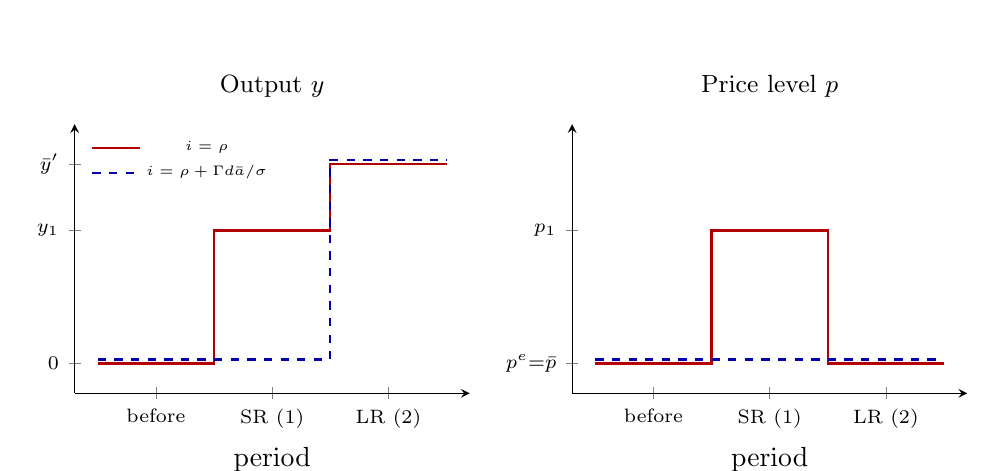
\begin{tikzpicture}
\begin{axis}[name=py,width=6.6cm,height=5cm,axis lines=left,xmin=-0.2,xmax=3.2,ymin=-0.15,ymax=1.2,
  xlabel={period},xtick={0.5,1.5,2.5},xticklabels={before,SR (1),LR (2)},ytick={0,0.6667,1},
  yticklabels={$0$,$y_1$,$\bar y'$},title={\small Output $y$},every tick label/.append style={font=\scriptsize},
  legend style={font=\tiny,draw=none,at={(0.02,0.98)},anchor=north west}]
\addplot[thick,red!70!black,const plot] coordinates {(0,0)(1,0.6667)(2,1)(3,1)};
\addplot[thick,blue!70!black,dashed,const plot] coordinates {(0,0.02)(1,0.02)(2,1.02)(3,1.02)};
\legend{$i=\rho$,$i=\rho+\Gamma d\bar a/\sigma$}
\end{axis}
\begin{axis}[at={(py.east)},anchor=west,xshift=1.3cm,width=6.6cm,height=5cm,axis lines=left,xmin=-0.2,xmax=3.2,
  ymin=-0.15,ymax=1.2,xlabel={period},xtick={0.5,1.5,2.5},xticklabels={before,SR (1),LR (2)},ytick={0,0.6667},
  yticklabels={$p^e{=}\bar p$,$p_1$},title={\small Price level $p$},every tick label/.append style={font=\scriptsize}]
\addplot[thick,red!70!black,const plot] coordinates {(0,0)(1,0.6667)(2,0)(3,0)};
\addplot[thick,blue!70!black,dashed,const plot] coordinates {(0,0.02)(3,0.02)};
\end{axis}
\end{tikzpicture}\\
{\footnotesize Figure 5. Solid: no response, a boom with a price surprise in the short run. Dashed: the rate rise
keeps $y=y_n=y_e$ and $p=p^e$ in the short run; in the long run both paths reach $\bar y'$ and $\bar p$.}
\end{center}
\intuicao{The central bank's job is to set the real rate to the one the economy would have with flexible prices.
Good news about the future raises that rate; tracking it is not ``fighting'' the news.}
\refbib{Benigno (2015) \S6.3, Fig.~8, pp.~511--513 (optimal response to expected productivity); \S5 ($r_n$); \S11, p.~522
(no trade-off when $y_n=y_e$).}
\rubrica{
\item Raise $i$, with the mechanism (AD back through $(y_n,p^e)$): 0.3 pt.
\item Size $\Gamma d\bar a/\sigma$, read as the rise in $r_n$: 0.2 pt.
\item Cost: none, both gaps closed, because the shock is efficient ($y_n=y_e$); claim rejected: 0.3 pt.
\item Paths SR/LR with and without the response: 0.2 pt (0.1 if the long run is missing).
\item Cutting $i$: max.\ 0.2 pt on the item. ``Cost: a recession'' (a trade-off asserted): max.\ 0.5 pt.
}
\gap{Prova 01, 3.a--3.b: which bar moves which curve; sign of the policy response to a pure AD shift; the cost
of a response when there is no trade-off.}
\end{sol}

\sub{3.c}{1 point} Suppose the monetary authority represents society's preferences by the quadratic
loss function, with parameter $\phi\geq0$,
\begin{equation}
L=\frac12\left(y-y_e\right)^2+\frac{\phi}{2\kappa}\left(p-p^e\right)^2 . \tag{LF}\label{q3:LF}
\end{equation}
In the same period as the news of item 3.a, the government temporarily raises a tax on firms' sales
revenue (an IPI-like tax), which raises the current mark-up by $d\mu>0$; the long-run mark-up $\bar\mu$
does not change. Derive the optimal monetary-policy rule (IT), find the optimal $y$, $p$ and $i$, and
show graphically the optimal policy. Discuss how your answer depends on $\phi$, separating the part of
the optimal response that answers the news from the part that answers the mark-up shock.
\resolespaco[8cm]
\begin{sol}
\begin{notacao}
\item As in 3.a--3.b. New: $\phi\ge0$, the weight on price surprises in \eqref{q3:LF}.
\item $m\equiv\frac{d\mu}{\sigma^{-1}+\eta}>0$: the fall in natural output caused by the tax.
$y_n'$: natural output after the tax.
\item $y^\ast$, $p^\ast$, $i^\ast$: optimal output, price level and interest rate; $O=(y^\ast,p^\ast)$.
\item $N$, $y_N$: the point on the new AS, and its output, reached when $i$ only offsets the news.
\end{notacao}
\passo{what the tax moves}{Differentiate \eqref{q3:YN} with respect to the current mark-up:}
\begin{equation}
y_n'=-\frac{d\mu}{\sigma^{-1}+\eta}=-m<0. \label{q3c:yn}
\end{equation}
Current natural output falls, so \textbf{AS shifts up/left} through $(y_n',p^e)$. $y_e$ in
\eqref{q3:ye} has no $\mu$: $y_e=0$ is unchanged. Now $y_n\neq y_e$: the tax is an
\emph{inefficient} shock. $\bar\mu$ is unchanged, so by \eqref{q3:ybar} the AD shift is only the
news ($\bar y=\Gamma d\bar a$, \eqref{q3a:dybar}).
\passo{AS is the constraint}{The central bank moves AD with $i$; for any point on AS there is an
$i$ that puts AD through it. AS, with $p^e$ preset, is what policy cannot move within the period:
it is the feasible set. So choose $y$ on AS and recover $i$ from AD. By \eqref{q3:AS} with
\eqref{q3c:yn}, the constraint is}
\begin{equation}
p-p^e=\kappa\,(y-y_n'). \label{q3c:AS}
\end{equation}
Substitute \eqref{q3c:AS} into \eqref{q3:LF}:
\begin{align}
L(y) &= \tfrac12(y-y_e)^2+\tfrac{\phi}{2\kappa}\big[\kappa\,(y-y_n')\big]^2\nonumber\\
&= \tfrac12(y-y_e)^2+\tfrac{\phi}{2\kappa}\kappa^2(y-y_n')^2\nonumber\\
&= \tfrac12(y-y_e)^2+\tfrac{\phi\kappa}{2}(y-y_n')^2 . \label{q3c:L}
\end{align}
\passo{targeting rule}{Differentiate \eqref{q3c:L} and set it to zero:}
\begin{equation}
\frac{dL}{dy}=(y-y_e)+\phi\kappa\,(y-y_n')=0. \label{q3c:foc}
\end{equation}
By \eqref{q3c:AS}, $\kappa(y-y_n')=p-p^e$. Substitute this into \eqref{q3c:foc}:
\begin{equation}
\boxed{(y-y_e)+\phi\,(p-p^e)=0}\qquad\text{(IT: a line through $(y_e,p^e)$ with slope $-1/\phi$).} \label{q3c:IT}
\end{equation}
SOC: from \eqref{q3c:L}, $d^2L/dy^2=1+\phi\kappa>0$.
\passo{optimal point}{Solve \eqref{q3c:foc} for $y$:}
\begin{align}
y(1+\phi\kappa) &= y_e+\phi\kappa\,y_n'\nonumber\\
y^\ast &= \frac{y_e+\phi\kappa\,y_n'}{1+\phi\kappa}. \label{q3c:ystar}
\end{align}
Substitute $y_e=0$ and \eqref{q3c:yn} into \eqref{q3c:ystar}:
\begin{align}
y^\ast &= \frac{(0)+\phi\kappa\,(-m)}{1+\phi\kappa}\nonumber\\
&= \boxed{-\frac{\phi\kappa}{1+\phi\kappa}\,m<0} \label{q3c:ystarm}
\end{align}
Substitute \eqref{q3c:ystarm} and \eqref{q3c:yn} into \eqref{q3c:AS}:
\begin{align}
p^\ast-p^e &= \kappa(y^\ast-y_n')\nonumber\\
&= \kappa\left[\left(-\frac{\phi\kappa}{1+\phi\kappa}\,m\right)-(-m)\right]\nonumber\\
&= \kappa\left(m-\frac{\phi\kappa\,m}{1+\phi\kappa}\right)\nonumber\\
&= \boxed{\frac{\kappa}{1+\phi\kappa}\,m>0}. \label{q3c:pstar}
\end{align}
Check in \eqref{q3c:IT}:
\begin{align*}
(y^\ast-y_e)+\phi(p^\ast-p^e) &= \left[\left(-\frac{\phi\kappa}{1+\phi\kappa}\,m\right)-(0)\right]
+\phi\left(\frac{\kappa}{1+\phi\kappa}\,m\right)\\
&= \frac{-\phi\kappa m+\phi\kappa m}{1+\phi\kappa}=0\ \checkmark
\end{align*}
The bank splits the shock: output below efficient \emph{and} prices above $p^e$.
\passo{optimal rate}{Evaluate AD \eqref{q3:ADr} at $(y^\ast,p^\ast)$, with $\bar y=\Gamma d\bar a$,
and solve for $i^\ast$:}
\begin{align}
(y^\ast) &= (\Gamma\,d\bar a)-\sigma(i^\ast-\rho)-\sigma\big((p^\ast)-p^e\big)\nonumber\\
\sigma(i^\ast-\rho) &= \Gamma\,d\bar a-y^\ast-\sigma(p^\ast-p^e)\nonumber\\
i^\ast &= \rho+\frac{\Gamma\,d\bar a-y^\ast}{\sigma}-(p^\ast-p^e). \label{q3c:igen}
\end{align}
Substitute \eqref{q3c:ystarm} and \eqref{q3c:pstar} into \eqref{q3c:igen}:
\begin{align}
i^\ast &= \rho+\frac{\Gamma\,d\bar a-\left(-\frac{\phi\kappa}{1+\phi\kappa}\,m\right)}{\sigma}
-\left(\frac{\kappa}{1+\phi\kappa}\,m\right)\nonumber\\
&= \rho+\frac{\Gamma\,d\bar a}{\sigma}+\frac{\phi\kappa m}{\sigma(1+\phi\kappa)}-\frac{\kappa m}{1+\phi\kappa}. \label{q3c:i4}
\end{align}
Put the last two terms of \eqref{q3c:i4} over the common denominator $\sigma(1+\phi\kappa)$:
\begin{equation}
\boxed{i^\ast=\rho+\underbrace{\frac{\Gamma\,d\bar a}{\sigma}}_{\text{news}}
+\underbrace{\frac{\kappa\,m\,(\phi-\sigma)}{\sigma(1+\phi\kappa)}}_{\text{mark-up}}} \label{q3c:istar}
\end{equation}
\passo{the news part does not depend on $\phi$}{The news moves neither $y_n$ nor $y_e$, so by
\eqref{q3c:ystar} it does not move the optimal point $O=(y^\ast,p^\ast)$ on AS. The bank simply
undoes the AD shift, $di=\Gamma d\bar a/\sigma$ in \eqref{q3c:istar}, for \emph{any} $\phi$, exactly
as in \eqref{q3b:i}.}
\passo{the mark-up part depends on $\phi$ against $\sigma$}{Substitute the news-offset rate
\eqref{q3b:i} and $\bar y=\Gamma d\bar a$ into AD \eqref{q3:ADr}: AD is back at AD$_0$. Then
substitute \eqref{q3c:AS} for $p-p^e$ to find the point $N$:}
\begin{align}
y &= (\Gamma\,d\bar a)-\sigma\left(\frac{\Gamma\,d\bar a}{\sigma}\right)-\sigma(p-p^e)\nonumber\\
&= -\sigma(p-p^e)\nonumber\\
y &= -\sigma\big[\kappa\,(y-y_n')\big]\nonumber\\
y_N &= \frac{\sigma\kappa}{1+\sigma\kappa}\,y_n'. \label{q3c:yN}
\end{align}
Subtract \eqref{q3c:yN}, with $y_n'=-m$, from \eqref{q3c:ystarm}:
\begin{align}
y^\ast-y_N &= \left(-\frac{\phi\kappa}{1+\phi\kappa}\,m\right)-\frac{\sigma\kappa}{1+\sigma\kappa}\,(-m)\nonumber\\
&= -\frac{\phi\kappa m}{1+\phi\kappa}+\frac{\sigma\kappa m}{1+\sigma\kappa}\nonumber\\
&= \frac{\kappa m(\sigma-\phi)}{(1+\phi\kappa)(1+\sigma\kappa)}. \label{q3c:diff}
\end{align}
If $\phi>\sigma$ (the IT line is flatter than AD), \eqref{q3c:diff} is negative: the bank raises $i$
further and accepts a deeper output loss for less price movement; if $\phi<\sigma$ it raises $i$ by
less than the news alone requires. Limits of \eqref{q3c:ystarm}, \eqref{q3c:pstar} and
\eqref{q3c:istar}:
\begin{align*}
\phi\to\infty\ \text{(strict price stability)}:&\quad y^\ast=y_n',\quad p^\ast=p^e,\quad
i^\ast=\rho+\frac{\Gamma d\bar a+m}{\sigma},\\
\phi=0:&\quad y^\ast=y_e,\quad p^\ast=p^e+\kappa m,\quad i^\ast=\rho+\frac{\Gamma d\bar a}{\sigma}-\kappa m.
\end{align*}
\passo{trade-off}{Unlike 3.b there is a trade-off: $y_n'\neq y_e$, so no rate closes both gaps;
$\phi$ chooses where on AS to sit.}
\begin{center}\begin{minipage}{\linewidth}\centering
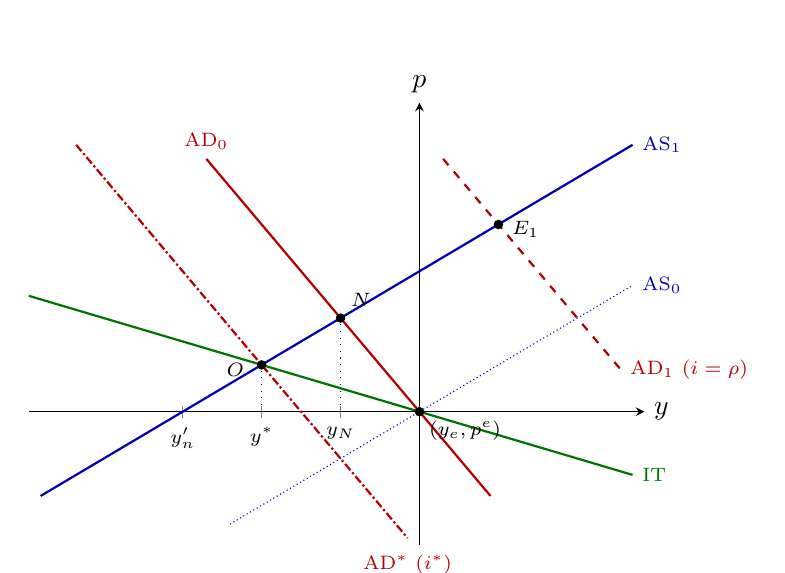
\begin{tikzpicture}
\begin{axis}[width=9.4cm,height=7.2cm,axis lines=middle,xmin=-1.65,xmax=0.95,ymin=-0.95,ymax=2.2,clip=false,
  xlabel={$y$},ylabel={$p$},xtick={-1,-0.6667,-0.3333},xticklabels={$y_n'$,$y^\ast$,$y_N$},ytick=\empty,
  every tick label/.append style={font=\scriptsize},x label style={anchor=west},y label style={anchor=south}]
\addplot[densely dotted,blue!70!black,domain=-0.8:0.9]{x};
\addplot[thick,blue!70!black,domain=-1.6:0.9]{x+1};
\addplot[thick,green!45!black,domain=-1.65:0.9]{-x/2};
\addplot[thick,red!70!black,dashed,domain=0.1:0.85]{2-2*x};
\addplot[thick,red!70!black,domain=-0.9:0.3]{-2*x};
\addplot[thick,red!70!black,densely dashdotted,domain=-1.45:-0.05]{-1-2*x};
\node[font=\scriptsize,blue!70!black,anchor=west] at (axis cs:0.9,0.9){AS$_0$};
\node[font=\scriptsize,blue!70!black,anchor=west] at (axis cs:0.9,1.9){AS$_1$};
\node[font=\scriptsize,green!45!black,anchor=west] at (axis cs:0.9,-0.45){IT};
\node[font=\scriptsize,red!70!black,anchor=west] at (axis cs:0.85,0.3){AD$_1$ ($i=\rho$)};
\node[font=\scriptsize,red!70!black,anchor=south] at (axis cs:-0.9,1.8){AD$_0$};
\node[font=\scriptsize,red!70!black,anchor=north] at (axis cs:-0.05,-0.95){AD$^\ast$ ($i^\ast$)};
\addplot[only marks,mark=*,mark size=1.5pt]coordinates{(0.3333,1.3333)(-0.3333,0.6667)(-0.6667,0.3333)(0,0)};
\node[font=\scriptsize,anchor=west] at (axis cs:0.35,1.3){$E_1$};
\node[font=\scriptsize,anchor=south west] at (axis cs:-0.33,0.68){$N$};
\node[font=\scriptsize,anchor=east] at (axis cs:-0.7,0.3){$O$};
\node[font=\scriptsize,anchor=north west] at (axis cs:0,0){$(y_e,p^e)$};
\draw[dotted](axis cs:-0.6667,0)--(axis cs:-0.6667,0.3333);
\draw[dotted](axis cs:-0.3333,0)--(axis cs:-0.3333,0.6667);
\end{axis}
\end{tikzpicture}\\
{\footnotesize Figure 6. The tax shifts AS from AS$_0$ to AS$_1$ (through $(y_n',p^e)$); the news shifts AD from AD$_0$ to
AD$_1$. With $i=\rho$ the economy is at $E_1$. Offsetting the news alone brings AD back to AD$_0$ and the economy to
$N$. The optimum $O$ is where AS$_1$ meets the IT line; drawn for $\phi=2>\sigma=0.5$, so the bank raises $i$ beyond
the news offset, to AD$^\ast$. ($\kappa=1$, $\Gamma d\bar a=m=1$.)}
\end{minipage}\end{center}
\intuicao{Two shocks, two different jobs. The news is a demand shock with no trade-off: offset it fully. The tax is a
cost shock that drives a wedge between natural and efficient output: no rate fixes both gaps, so the convex loss
spreads the miss, and $\phi$ says how much of it goes into prices.}
\refbib{Benigno (2015) \S11, eqs.~(33)--(35), Fig.~14, pp.~521--523; \S7, Fig.~9, pp.~513--514 (mark-up shocks; taxes in
$1+\mu$); \S4.4, p.~509.}
\rubrica{
\item AS shifts up/left, $y_e$ does not move, AD shift from the news only: 0.15 pt.
\item Why AS is the constraint; substitution into $L$: 0.15 pt.
\item Targeting rule $(y-y_e)+\phi(p-p^e)=0$ from $dL/dy=0$: 0.2 pt.
\item $y^\ast$, $p^\ast$: 0.15 pt. $i^\ast$ with its two components: 0.15 pt.
\item Role of $\phi$: news part independent of $\phi$; mark-up part signed by $\phi-\sigma$; a limit case: 0.1 pt.
\item Graph (AS$_1$, IT, AD before/after, $O$ labelled): 0.1 pt.
\item Differentiating in $i$ with AD as the constraint, or targeting $y_n$ instead of $y_e$: max.\ 0.4 pt. Claiming the whole
response (news included) depends on $\phi$ versus $\sigma$: max.\ 0.6 pt.
}
\gap{Prova 01, 3.c: $dL/dy=0$ along AS not used; the response to news wrongly made to depend on $\phi$.}
\end{sol}

\ifsolucoes\else
\vfill
\begin{center}\footnotesize\textit{End of exam.}\end{center}
\fi

\end{document}
"
% Check fonts: pdffonts <file>.pdf  (all Type 1).
% Every closed form and number in the key: python simulado_codigo/check_simulado_04.py
% Solution format (rules/00_estilo_avaliacao.md §4): each solution opens with a Notation list;
% every equation used later is numbered and cited with \eqref; one operation per displayed line.
% Numbering: Q1 solutions use (G1), (G2)...; Q2 keeps the statement's (1)-(4) and continues from
% (5); Q3 keeps the statement's (AD), (AS), (YN), (LF) and continues the numeric sequence.
% =============================================================================
\documentclass[11pt,a4paper]{article}
\usepackage[utf8]{inputenc}
\usepackage[T1]{fontenc}
\usepackage{lmodern}   % Type 1 vector fonts (replaces PK bitmaps)
\usepackage{cmap}      % ToUnicode CMap -> copyable text and accents
\usepackage[english]{babel}
\usepackage{amsmath,amssymb,amsfonts}
\usepackage[a4paper,margin=2.2cm]{geometry}
\usepackage{enumitem}
\usepackage{fancyhdr}
\usepackage{comment}
% Private cut file per build (sibling sources build in this folder). comment.sty resets
% \CommentCutFile from \DefaultCutFileName at every included environment, so redefine that.
\def\DefaultCutFileName{\def\CommentCutFile{\jobname.cut}}
\usepackage{xcolor}
\usepackage{microtype}
\usepackage{booktabs}
\usepackage{needspace}
\usepackage{pgfplots}
\pgfplotsset{compat=1.18}
\usetikzlibrary{arrows.meta}

% ====================== CONFIGURATION ======================
\newif\ifsolucoes
\ifdefined\withsolutions\solucoestrue\else\solucoesfalse\fi

\newcommand{\disciplina}{Macroeconomics I --- MPE Insper}
\newcommand{\listatema}{Mock Exam 4}

% ====================== MACHINERY ======================
\ifsolucoes\includecomment{sol}\else\excludecomment{sol}\fi

\pagestyle{fancy}\fancyhf{}
\lhead{\footnotesize\disciplina}
\rhead{\footnotesize \listatema\ifsolucoes{} --- Solutions and Rubric\fi}
\cfoot{\footnotesize\thepage}
\renewcommand{\headrulewidth}{0.3pt}
\setlength{\headheight}{14pt}
\setlist{topsep=2pt,itemsep=2pt}

% \questao{number}{points}{statement}
\newcommand{\questao}[3]{\Needspace{12\baselineskip}\bigskip\noindent
  {\large\bfseries\color{blue!55!black}Question #1}\ \textbf{(#2 points)}\par\smallskip\noindent #3\par}
% \item-like heading: \sub{2.a}{1 point}
\newcommand{\sub}[2]{\Needspace{8\baselineskip}\par\medskip\noindent\textbf{#1 (#2)}~}
\newcommand{\resolespaco}[1][6cm]{\ifsolucoes\else\par\textit{Solution:}\vspace{#1}\par\fi}
\newcommand{\passo}[2]{\par\smallskip\noindent\textbf{Step --- #1.}~#2}
\newcommand{\intuicao}[1]{\par\smallskip\noindent\textit{Intuition.}~#1}
\newcommand{\refbib}[1]{\par\smallskip\noindent{\footnotesize\color{black!60}\textbf{Ref:} #1}}
\newcommand{\gap}[1]{\par\smallskip\noindent{\footnotesize\color{red!55!black}\textbf{Gap targeted:} #1}}
\newcommand{\trap}[1]{\par\smallskip\noindent{\small\color{red!55!black}\#~#1}}
\newcommand{\rubrica}[1]{\par\smallskip\noindent\textbf{Grading rubric.}\begin{itemize}[leftmargin=1.4em,topsep=1pt]#1\end{itemize}}
\newenvironment{notacao}{\par\smallskip\noindent\textbf{Notation.}\begin{itemize}[leftmargin=1.4em,topsep=1pt,itemsep=0pt]\small}{\end{itemize}}
\allowdisplaybreaks

% =============================================================================
\begin{document}
\begin{center}
  {\Large\bfseries \disciplina}\\[2pt]
  {\large \listatema\ (Simulado 4) --- 2026, 3rd term}\ifsolucoes\\[2pt]\textit{Solutions and Grading Rubric}\fi
\end{center}
\vspace{2pt}

{\footnotesize\noindent\textbf{Instructions.} Three questions, 10 points in total. Suggested time:
2 hours, closed book, non-programmable calculator allowed. Show every step: a number or a formula
without the argument that produces it earns little. When an item says \emph{explain},
\emph{justify} or \emph{show graphically}, the explanation and the graph are graded on their own
lines: label the axes and every curve, mark the initial and the new point, and indicate the
direction of every shift. Where an item lists several approaches or several choice variables,
answer \emph{each} of them. Box your final answers. Notation: Kurlat (2020) in Questions 1--2,
Benigno (2015) in Question 3.\par}

% =============================================================================
\renewcommand{\theequation}{G\arabic{equation}}% Q1 solution equations: (G1), (G2)...
\questao{1}{1.5}{A simplified economy has, at first, no government. Values are in R\$ million
for one year. A coffee farm in Minas Gerais (Firm F) grows beans worth 400 and sells all of them
to a roastery (Firm R); F uses no inputs and pays 250 in wages. Firm R buys the 400 of beans and
imports packaging worth 100 from abroad; it sells roasted coffee worth 700 to domestic households
and worth 200 to foreign buyers, and pays 300 in wages. Each firm keeps whatever is left as profit.}

\sub{1.a}{0.5 point} Calculate the GDP of this economy by the product, the income and the
expenditure approaches, explaining precisely the concept used in each. Explain why the imported
packaging does not count in GDP, although Firm R used it to produce.
\resolespaco[5.5cm]
\begin{sol}
\begin{notacao}
\item F, R: the coffee farm and the roastery. All values in R\$ million for one year.
\item $VA_j\ge0$: value added of firm $j$, its production minus the intermediate inputs it uses up.
\item $W_j\ge0$: wages paid by firm $j$. $\Pi_j$: its profit (operating surplus), whatever is left
after wages; it can be of either sign.
\item $C$, $I$, $G$: household consumption, investment and government purchases (final domestic
uses). $X\ge0$, $M\ge0$: exports and imports. In 1.a, $I=G=0$.
\end{notacao}
\passo{0, the definitions used below}{GDP is the market value of the \emph{final} goods and
services produced in the territory in the year. It is computed three ways, which must agree:}
\begin{align}
\text{GDP} &= \textstyle\sum_j VA_j, \label{q1:prod}\\
VA_j &= \text{production}_j-\text{intermediate inputs}_j, \label{q1:va}\\
\Pi_j &= VA_j-W_j, \label{q1:profit}\\
\text{GDP} &= \textstyle\sum_j (W_j+\Pi_j), \label{q1:inc}\\
\text{GDP} &= C+I+G+X-M. \label{q1:exp}
\end{align}
\passo{product (value added)}{F uses no inputs; R uses the beans and the imported packaging.
Using \eqref{q1:va} for each firm:}
\begin{align}
VA_F &= 400-0=400, \label{q1a:vaF}\\
VA_R &= (700+200)-400-100\nonumber\\
&= 900-500\nonumber\\
&= 400. \label{q1a:vaR}
\end{align}
Summing \eqref{q1a:vaF} and \eqref{q1a:vaR} with \eqref{q1:prod}:
\begin{equation}
\text{GDP}=400+400=\boxed{800}. \label{q1a:gdp}
\end{equation}
\passo{income (factor payments)}{Profit is what is left of value added after wages. Using
\eqref{q1:profit} with \eqref{q1a:vaF} and \eqref{q1a:vaR}:}
\begin{align}
\Pi_F &= 400-250=150, \label{q1a:piF}\\
\Pi_R &= 400-300=100. \label{q1a:piR}
\end{align}
Add wages and profits, then apply \eqref{q1:inc}:
\begin{align*}
W_F+W_R &= 250+300=550,\\
\Pi_F+\Pi_R &= 150+100=250,\\
\text{GDP} &= 550+250=\boxed{800}.
\end{align*}
\passo{expenditure (final uses)}{The final uses are $C=700$, $I=0$, $G=0$, $X=200$ and
$M=100$. By \eqref{q1:exp}:}
\[
\text{GDP}=700+0+0+200-100=\boxed{800}.
\]
\passo{imports}{The packaging was produced abroad: its 100 is \emph{foreign} value added. In the
product approach it is an intermediate input of R and is subtracted from R's production in
\eqref{q1a:vaR}. In the expenditure approach \eqref{q1:exp}, $C$ and $X$ are measured at purchaser
prices and already contain the packaging, so $-M$ takes it back out. GDP measures what is produced
\emph{in the territory}.}
\trap{Adding sales, $400+900=1300$, counts the beans twice (once as F's sale, once inside R's price) and
counts foreign packaging. The three approaches agree because they are three ways of adding up the same
value added.}
\intuicao{Every real that a final buyer pays for coffee ends up as somebody's income: F's workers and
owners, R's workers and owners, or the foreign packaging producer. Take the foreigner out and the three
columns must match.}
\refbib{Kurlat \S1.1, pp.~15--21 (value added, the three approaches, imports).}
\rubrica{
\item Each approach with the right concept and the number 800: 0.15 pt each (0.45).
\item Why imports are excluded (foreign value added; $-M$ corrects purchaser prices): 0.05 pt.
\item Only one approach, number right: max.\ 0.2 pt. Summing sales (1300) or forgetting $-M$ (900): 0 for that line.
}
\end{sol}

\sub{1.b}{0.5 point} Suppose instead that in the same year households buy only 600 of roasted
coffee. Firm R produces exactly as before and keeps the remaining roasted coffee in its warehouse at
the end of the year, valued at its selling price. Nothing else changes. Calculate, justifying, the
GDP by the product, income and expenditure approaches, compare it with the value in 1.a and explain
what the comparison indicates. Then explain what the sale of that stock to households in the
following year adds to the following year's GDP, other things equal.
\resolespaco[6cm]
\begin{sol}
\begin{notacao}
\item As in 1.a. New: $\Delta\text{inventories}$, the change in R's stock of unsold roasted coffee
during the year, valued at its selling price. It is part of $I$ and can be negative (a drawdown).
\end{notacao}
\passo{what changed}{R's production is unchanged; only its destination moved: households,
exports, and the part left unsold in the warehouse.}
\begin{equation}
\text{production}_R=600+200+100=900. \label{q1b:prodR}
\end{equation}
An unsold good that was produced is a \textbf{change in inventories}, a component of investment:
\begin{equation}
I=\Delta\text{inventories}=100. \label{q1b:inv}
\end{equation}
\passo{product}{F is unchanged, $VA_F=400$ by \eqref{q1a:vaF}. Using \eqref{q1:va} with
\eqref{q1b:prodR}:}
\begin{align*}
VA_R &= 900-400-100\\
&= 400.
\end{align*}
By \eqref{q1:prod}, GDP $=400+400=\boxed{800}$.
\passo{income}{R's operating surplus is measured on production, the stock valued at 100. Using
\eqref{q1:profit}:}
\begin{align*}
\Pi_R &= 900-500-300\\
&= 100.
\end{align*}
Wages are $250+300=550$ and profits $150+100=250$, with $\Pi_F$ from \eqref{q1a:piF}. By
\eqref{q1:inc}, GDP $=550+250=\boxed{800}$.
\passo{expenditure}{Now $C=600$, $I=100$ from \eqref{q1b:inv}, $G=0$, $X=200$, $M=100$. By
\eqref{q1:exp}:}
\[
\text{GDP}=600+100+0+200-100=\boxed{800}.
\]
\passo{comparison}{GDP is the same as \eqref{q1a:gdp}: \textbf{GDP measures production, not sales}.
Only the composition of final demand moved, $C\downarrow100$ and $I\uparrow100$. A firm that cannot
sell is recorded as having invested in its own stock (involuntary, in this case).}
\passo{next year}{Households buy the 100 from stock, so $C$ rises by 100 and inventory investment
is $-100$ (a drawdown). The net contribution to next year's GDP, by \eqref{q1:exp}:}
\begin{align*}
\Delta C &= +100,\\
\Delta I=\Delta\text{inventories} &= -100,\\
\Delta\text{GDP} &= 100-100=\boxed{0}.
\end{align*}
The coffee was counted in the year it was produced; counting it again when sold would double-count it.
\intuicao{Inventories are the entry that makes the expenditure column add up when sales and production
differ. Without it the expenditure side would read $600+200-100=700\neq800$.}
\refbib{Kurlat \S1.1, p.~18 (inventories and their drawdown), pp.~15--21.}
\rubrica{
\item Three approaches with 800 and the inventory entry in $I$: 0.1 pt each (0.3).
\item Comparison: production vs sales, $C$ replaced by $I$: 0.1 pt.
\item Next year: $+C$, $-I$, net zero, with the reason: 0.1 pt.
\item GDP $=700$ (unsold output treated as not produced): max.\ 0.1 pt. One approach only: max.\ 0.25 pt.
}
\end{sol}

\sub{1.c}{0.5 point} Return to the situation of 1.a. The government now collects a lump-sum tax
of 200 from households and uses it to: (i) pay 120 in wages to nurses in public clinics, which treat
patients free of charge; (ii) buy 30 of imported medicines, handed out free at those clinics;
(iii) pay 50 in cash transfers to low-income families (Bolsa Fam\'ilia). Households' purchases of
roasted coffee stay at 700 and nothing else changes. Calculate, justifying, the GDP by the product,
income and expenditure approaches, compare it with 1.a and explain what the comparison indicates.
Explain why GDP does not rise by 200.
\resolespaco[6.5cm]
\begin{sol}
\begin{notacao}
\item As in 1.a. New: the public clinics as a producer, with value added $VA_{\text{clinics}}$.
\item $T=200$: the lump-sum tax. $TR=50$: the cash transfers. Both are flows between households and
government with nothing produced in exchange.
\end{notacao}
\passo{valuing a free service}{Public health care has no market price, so its output is valued
\textbf{at cost}, wages plus inputs:}
\begin{equation}
\text{output}_{\text{clinics}}=120+30=150. \label{q1c:out}
\end{equation}
The medicines are an intermediate input of the clinics. Using \eqref{q1:va} with \eqref{q1c:out}:
\begin{equation}
VA_{\text{clinics}}=150-30=120. \label{q1c:va}
\end{equation}
\passo{product}{Sum \eqref{q1a:vaF}, \eqref{q1a:vaR} and \eqref{q1c:va} with \eqref{q1:prod}:}
\begin{equation}
\text{GDP}=400+400+120=\boxed{920}. \label{q1c:gdp}
\end{equation}
\passo{income}{The clinics have no operating surplus: output is defined as cost, so by
\eqref{q1:profit} their profit is $120-120=0$. Adding up and applying \eqref{q1:inc}:}
\begin{align*}
\text{wages} &= 250+300+120=670,\\
\text{profits} &= 150+100+0=250,\\
\text{GDP} &= 670+250=\boxed{920}.
\end{align*}
\passo{expenditure}{$G=150$ is the clinics' output \eqref{q1c:out}, consumed on behalf of
households. Imports now include the medicines:}
\[
M=100+30=130.
\]
With $C=700$, $I=0$ and $X=200$, by \eqref{q1:exp}:
\[
\text{GDP}=700+0+150+200-130=\boxed{920}.
\]
\passo{what is left out, and why}{\textbf{The tax} (200) is a transfer from households to the
government, not a payment for a good: it is in no column. \textbf{Transfers} (50) buy nothing in
exchange: they are not in $G$ and not factor income (if the families spent them, the spending would
appear in $C$; here $C$ is unchanged by assumption). \textbf{Imported medicines} (30) enter $G$ but are
removed by $-M$: foreign value added.}
\passo{comparison}{Subtract \eqref{q1a:gdp} from \eqref{q1c:gdp}:}
\[
\Delta\text{GDP}=920-800=\boxed{120},
\]
the value added of public health care \eqref{q1c:va}, i.e.\ the nurses' wages. Not by 200 (the tax
is a financing flow), not by 150 (30 of $G$ is imported), not by 50 (transfers are redistribution).
\intuicao{Valuing government output at cost has a consequence: measured public-sector value added equals
its wage bill. If the nurses treated twice as many patients for the same pay, GDP would not record it.}
\refbib{Kurlat \S1.1, p.~20 (Example 1.7, government output at cost; Example 1.8, transfers), pp.~15--21.}
\rubrica{
\item Three approaches with 920, clinics' output at cost and $VA=120$: 0.1 pt each (0.3).
\item Tax, transfers and imported medicines each correctly excluded, with the reason: 0.1 pt.
\item Comparison: $+120$ is the nurses' value added: 0.1 pt.
\item Transfers counted in $G$ (GDP 970) or tax counted (1000): max.\ 0.2 pt. Medicines not netted by $M$ (950): $-0.1$.
}
\gap{Prova 01, 1.b--1.c: the three approaches were asked and only one was given; the classification of a
final use (there: software as investment; here: inventories as investment, clinics' output as $G$).}
\end{sol}

% =============================================================================
\questao{2}{5.5}{Consider an economy described by the Solow model, in which the aggregate variables
satisfy:
\begin{align}
Y_t &= K_t^{\alpha}(A_tL_t)^{1-\alpha}, \tag{1}\label{q2:Y}\\
K_{t+1} &= (1-\delta)K_t+s\,Y_t, \tag{2}\label{q2:K}\\
L_{t+1} &= (1+n)L_t, \tag{3}\label{q2:L}\\
A_{t+1} &= (1+g)A_t, \tag{4}\label{q2:A}
\end{align}
with $\{\alpha,\delta,s\}\in(0,1)$ and $n,g\geq0$.}
\setcounter{equation}{4}\renewcommand{\theequation}{\arabic{equation}}% Q2-Q3 continue from (5)

\sub{2.a}{1 point} Define the stationary variables, per efficiency unit of labour, with a tilde
($\tilde k_t$, $\tilde y_t$), and find an expression for $\tilde k_{t+1}/\tilde k_t$ and then the
steady-state value of $\tilde k$, denoted $\tilde k_{SS}$. Show the steady state graphically. Along
the steady state, at what rates do output per worker $y_t=Y_t/L_t$ and aggregate output $Y_t$ grow?
Justify, and explain why output per worker is not a stationary variable here.
\resolespaco[7cm]
\begin{sol}
\begin{notacao}
\item $Y_t$, $K_t$, $C_t>0$: aggregate output, capital and consumption. $L_t>0$: number of workers.
\item $A_t>0$: labour-augmenting technology; $A_tL_t$ is labour in efficiency units.
\item $\alpha\in(0,1)$: elasticity of output with respect to capital (capital's income share).
$\delta\in(0,1)$: depreciation rate. $s\in(0,1)$: saving rate. $n\ge0$: labour-force growth rate.
$g\ge0$: growth rate of technology.
\item $\tilde k_t$, $\tilde y_t$, $\tilde c_t>0$: capital, output and consumption per efficiency unit
of labour. $k_t=K_t/L_t$, $y_t=Y_t/L_t$: per worker.
\item $\xi\equiv(1+g)(1+n)-(1-\delta)>0$: break-even investment per unit of $\tilde k$ (defined in
step 3). $\tilde k_{SS}$, $\tilde y_{SS}$: steady-state values.
\end{notacao}
\passo{stationary variables}{Technology and labour both grow, so the variables that settle down are
those per efficiency unit:}
\begin{equation}
\tilde k_t\equiv\frac{K_t}{A_tL_t},\qquad \tilde y_t\equiv\frac{Y_t}{A_tL_t},\qquad
\tilde c_t\equiv\frac{C_t}{A_tL_t}. \label{q2a:def}
\end{equation}
Divide \eqref{q2:Y} by $A_tL_t$ and use \eqref{q2a:def}:
\begin{align}
\tilde y_t &= \frac{K_t^{\alpha}(A_tL_t)^{1-\alpha}}{A_tL_t}\nonumber\\
&= K_t^{\alpha}(A_tL_t)^{-\alpha}\nonumber\\
&= \left(\frac{K_t}{A_tL_t}\right)^{\alpha}\nonumber\\
&= \tilde k_t^{\alpha}. \label{q2a:y}
\end{align}
\passo{law of motion}{Multiply \eqref{q2:A} by \eqref{q2:L}:}
\begin{align}
A_{t+1}L_{t+1} &= \big[(1+g)A_t\big]\big[(1+n)L_t\big]\nonumber\\
&= (1+g)(1+n)A_tL_t. \label{q2a:AL}
\end{align}
Divide \eqref{q2:K} by \eqref{q2a:AL}. The second line splits the fraction, the third uses
\eqref{q2a:def}, the fourth \eqref{q2a:y}:
\begin{align}
\tilde k_{t+1} &= \frac{(1-\delta)K_t+sY_t}{(1+g)(1+n)A_tL_t}\nonumber\\
&= \frac{(1-\delta)\frac{K_t}{A_tL_t}+s\frac{Y_t}{A_tL_t}}{(1+g)(1+n)}\nonumber\\
&= \frac{(1-\delta)\tilde k_t+s\tilde y_t}{(1+g)(1+n)}\nonumber\\
&= \frac{(1-\delta)\tilde k_t+s\tilde k_t^{\alpha}}{(1+g)(1+n)}. \label{q2a:lom}
\end{align}
Divide \eqref{q2a:lom} by $\tilde k_t$:
\begin{equation}
\boxed{\frac{\tilde k_{t+1}}{\tilde k_t}=\frac{1-\delta+s\,\tilde k_t^{\alpha-1}}{(1+g)(1+n)}} \label{q2a:ratio}
\end{equation}
\passo{steady state}{Set \eqref{q2a:ratio} equal to 1 and isolate the term in $\tilde k$:}
\begin{align*}
1 &= \frac{1-\delta+s\tilde k^{\alpha-1}}{(1+g)(1+n)}\\
(1+g)(1+n) &= 1-\delta+s\tilde k^{\alpha-1}\\
s\tilde k^{\alpha-1} &= (1+g)(1+n)-(1-\delta).
\end{align*}
Call the right side $\xi$; expanding the product,
\begin{equation}
\xi\equiv(1+g)(1+n)-(1-\delta)=n+g+ng+\delta\ (\approx n+g+\delta). \label{q2a:xi}
\end{equation}
Using \eqref{q2a:xi}:
\begin{align*}
s\tilde k^{\alpha-1} &= \xi\\
\tilde k^{1-\alpha} &= \frac{s}{\xi}.
\end{align*}
Raise both sides to the power $1/(1-\alpha)$:
\begin{equation}
\boxed{\tilde k_{SS}=\left(\frac{s}{(1+g)(1+n)-(1-\delta)}\right)^{\frac{1}{1-\alpha}}} \label{q2a:kss}
\end{equation}
Evaluate \eqref{q2a:y} at \eqref{q2a:kss}, writing its denominator as $\xi$ by \eqref{q2a:xi}:
\begin{align}
\tilde y_{SS} &= \tilde k_{SS}^{\alpha}\nonumber\\
&= \left[\left(\frac{s}{\xi}\right)^{\frac{1}{1-\alpha}}\right]^{\alpha}\nonumber\\
&= \left(\frac{s}{\xi}\right)^{\frac{\alpha}{1-\alpha}}. \label{q2a:yss}
\end{align}
Multiplying the condition $s\tilde k^{\alpha-1}=\xi$ by $\tilde k$ gives the steady state as
investment equal to break-even investment:
\begin{equation}
s\tilde k_{SS}^{\alpha}=\xi\,\tilde k_{SS}. \label{q2a:break}
\end{equation}
\passo{stability}{In \eqref{q2a:ratio}, $\alpha-1<0$, so $\tilde k_{t+1}/\tilde k_t$ falls as
$\tilde k_t$ rises: it is $>1$ below $\tilde k_{SS}$ and $<1$ above. The positive steady state is
unique and every $\tilde k_0>0$ converges to it. Graphically (Figure 1): investment per efficiency
unit $s\tilde k^{\alpha}$ against break-even investment $\xi\tilde k$, the two sides of
\eqref{q2a:break}; $\xi$ is the amount needed to equip the new workers ($n$), the new efficiency
units ($g$) and to replace depreciation ($\delta$).}
\passo{growth rates}{In the steady state $\tilde y=\tilde y_{SS}$ is constant. Invert
\eqref{q2a:def}:}
\begin{align}
y_t &= \frac{Y_t}{L_t}=A_t\,\tilde y_{SS}, \label{q2a:ypw}\\
Y_t &= A_tL_t\,\tilde y_{SS}. \label{q2a:Yagg}
\end{align}
Take ratios of consecutive periods, using \eqref{q2:A} in \eqref{q2a:ypw} and \eqref{q2a:AL} in
\eqref{q2a:Yagg}:
\begin{align*}
\frac{y_{t+1}}{y_t} &= \frac{A_{t+1}\,\tilde y_{SS}}{A_t\,\tilde y_{SS}}\\
&= \frac{\big[(1+g)A_t\big]\tilde y_{SS}}{A_t\,\tilde y_{SS}}\\
&= 1+g &&\Rightarrow\ y_t\text{ grows at }\boxed{g},\\
\frac{Y_{t+1}}{Y_t} &= \frac{A_{t+1}L_{t+1}\,\tilde y_{SS}}{A_tL_t\,\tilde y_{SS}}\\
&= \frac{\big[(1+g)(1+n)A_tL_t\big]\tilde y_{SS}}{A_tL_t\,\tilde y_{SS}}\\
&= (1+g)(1+n) &&\Rightarrow\ Y_t\text{ grows at }\boxed{(1+g)(1+n)-1=g+n+gn}.
\end{align*}
The same holds for $k_t=K_t/L_t$ ($g$) and $K_t$ ($g+n+gn$); $K/Y$ is constant.
\passo{why $y$ is not stationary}{Each period every worker supplies $1+g$ times more efficiency units.
Capital per worker must grow at $g$ just to keep pace, so per-worker variables have a trend; dividing by
$A_tL_t$ removes it. Long-run growth of $y$ comes only from $g$, which the model takes as given.}
\begin{center}
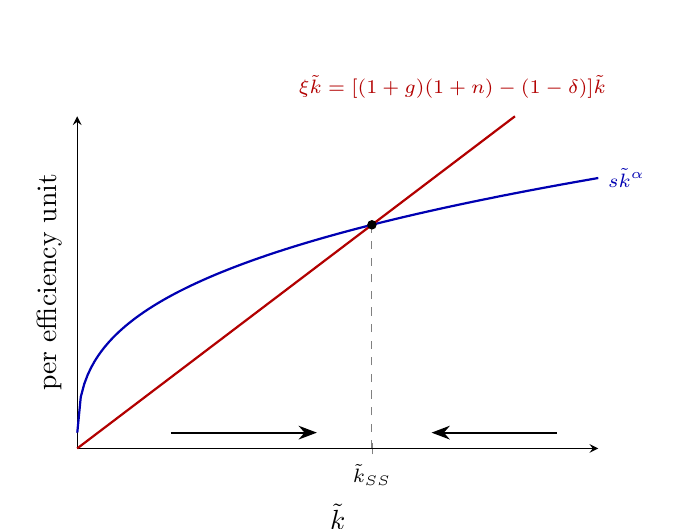
\begin{tikzpicture}
\begin{axis}[width=8.2cm,height=5.8cm,axis lines=left,xmin=0,xmax=5,ymin=0,ymax=0.42,clip=false,
  xlabel={$\tilde k$},ylabel={per efficiency unit},xtick={2.828},xticklabels={$\tilde k_{SS}$},ytick=\empty,
  every tick label/.append style={font=\scriptsize}]
\addplot[domain=0.001:5,samples=150,thick,blue!70!black]{0.2*x^(1/3)};
\addplot[domain=0:4.2,thick,red!70!black]{0.1*x};
\node[font=\scriptsize,blue!70!black,anchor=west] at (axis cs:5,0.342){$s\tilde k^{\alpha}$};
\node[font=\scriptsize,red!70!black,anchor=south] at (axis cs:3.6,0.43){$\xi\tilde k=[(1+g)(1+n)-(1-\delta)]\tilde k$};
\draw[dashed,gray](axis cs:2.828,0)--(axis cs:2.828,0.2828);
\addplot[only marks,mark=*,mark size=1.5pt]coordinates{(2.828,0.2828)};
\draw[-{Stealth},thick](axis cs:0.9,0.02)--(axis cs:2.3,0.02);
\draw[-{Stealth},thick](axis cs:4.6,0.02)--(axis cs:3.4,0.02);
\end{axis}
\end{tikzpicture}\\
{\footnotesize Figure 1. Steady state per efficiency unit. Left of $\tilde k_{SS}$ investment exceeds break-even
investment and $\tilde k$ rises; right of it, $\tilde k$ falls. (Drawn for $\alpha=1/3$, $s=0.2$, $\xi=0.1$.)}
\end{center}
\intuicao{Solow with technological progress is the no-progress model with one change of units: count
workers in efficiency units and the economy settles at a constant $\tilde k$; in per-worker units that same
point is a path growing at $g$.}
\refbib{Kurlat \S4.2, pp.~57--61 (law of motion, steady state, stability); \S4.5, pp.~69--72 (efficiency units,
balanced growth path).}
\rubrica{
\item Stationary variables defined and $\tilde y=\tilde k^{\alpha}$: 0.2 pt.
\item Ratio $\tilde k_{t+1}/\tilde k_t$ with $(1+g)(1+n)$ in the denominator: 0.3 pt.
\item $\tilde k_{SS}$: 0.2 pt. Diagram (axes, both curves named, $\tilde k_{SS}$ marked): 0.1 pt.
\item Growth rates of $y$ and $Y$ with the reason: 0.2 pt.
\item Dividing (2) by $A_tL_t$ instead of $A_{t+1}L_{t+1}$ (no $(1+g)(1+n)$): max.\ 0.5 pt. Working with $K/L$ as if stationary: max.\ 0.4 pt.
}
\end{sol}

\sub{2.b}{1 point} Show which saving rate maximises steady-state consumption per efficiency unit
of labour (the golden-rule rate, $s_{GR}$). Explain why the same $s_{GR}$ also maximises consumption
per worker at every date along the steady state, and how a faster rate of technological progress
$g$ changes $s_{GR}$ and $\tilde k_{GR}$. Give the economic intuition.
\resolespaco[7cm]
\begin{sol}
\begin{notacao}
\item As in 2.a. New: $\tilde c_{SS}(s)$, steady-state consumption per efficiency unit as a function
of the saving rate.
\item $f(\tilde k)\equiv\tilde k^{\alpha}$: output per efficiency unit, by \eqref{q2a:y}.
\item $s_{GR}\in(0,1)$, $\tilde k_{GR}>0$: golden-rule saving rate and capital per efficiency unit.
\item $c_t\equiv C_t/L_t$: consumption per worker. $A_0>0$: technology at date 0.
\end{notacao}
\passo{consumption in steady state}{Consumption is the part of output not saved:}
\begin{equation}
\tilde c_t=(1-s)\,\tilde y_t. \label{q2b:c}
\end{equation}
Substitute \eqref{q2a:yss} into \eqref{q2b:c}, carrying the exponent $\alpha$ of
$\tilde k_{SS}^{\alpha}$ through the substitution:
\begin{align}
\tilde c_{SS}(s) &= (1-s)\,\tilde k_{SS}^{\alpha}\nonumber\\
&= (1-s)\left[\left(\frac{s}{\xi}\right)^{\frac{1}{1-\alpha}}\right]^{\alpha}\nonumber\\
&= (1-s)\left(\frac{s}{\xi}\right)^{\frac{\alpha}{1-\alpha}}. \label{q2b:css}
\end{align}
\passo{first-order condition}{Take the log of \eqref{q2b:css}:}
\begin{equation}
\ln\tilde c_{SS}=\ln(1-s)+\frac{\alpha}{1-\alpha}\ln s-\frac{\alpha}{1-\alpha}\ln\xi. \label{q2b:log}
\end{equation}
Differentiate \eqref{q2b:log} with respect to $s$ and set it to zero:
\begin{equation}
\frac{d\ln\tilde c_{SS}}{ds}=-\frac{1}{1-s}+\frac{\alpha}{(1-\alpha)s}=0. \label{q2b:foc}
\end{equation}
Multiply \eqref{q2b:foc} by $(1-\alpha)s(1-s)>0$:
\begin{align*}
-(1-\alpha)s+\alpha(1-s) &= 0\\
\alpha(1-s) &= (1-\alpha)s\\
\alpha-\alpha s &= s-\alpha s\\
\alpha &= s.
\end{align*}
Hence
\begin{equation}
\boxed{s_{GR}=\alpha} \label{q2b:sgr}
\end{equation}
SOC: differentiate \eqref{q2b:foc} once more:
\[
\frac{d^2\ln\tilde c_{SS}}{ds^2}=-\frac{1}{(1-s)^2}-\frac{\alpha}{(1-\alpha)s^2}<0,
\]
so \eqref{q2b:sgr} is a maximum.
\passo{cross-check by $\tilde k$}{Substitute \eqref{q2a:y} into \eqref{q2b:c}, then use the
steady-state condition \eqref{q2a:break}, $s\tilde k^{\alpha}=\xi\tilde k$:}
\begin{align}
\tilde c &= (1-s)\big(\tilde k^{\alpha}\big)\nonumber\\
&= \tilde k^{\alpha}-s\tilde k^{\alpha}\nonumber\\
&= \tilde k^{\alpha}-\big(\xi\tilde k\big). \label{q2b:ck}
\end{align}
Maximise \eqref{q2b:ck} over $\tilde k$:
\begin{equation}
\boxed{f'(\tilde k_{GR})=\alpha\tilde k_{GR}^{\alpha-1}=\xi=(1+g)(1+n)-(1-\delta)} \label{q2b:mpk}
\end{equation}
The marginal product of capital equals break-even investment per unit of capital. Solve
\eqref{q2b:mpk} for $\tilde k_{GR}$:
\begin{equation}
\tilde k_{GR}^{1-\alpha}=\frac{\alpha}{\xi}. \label{q2b:kgr}
\end{equation}
Solve \eqref{q2a:break} for $s$ at $\tilde k_{GR}$ and use \eqref{q2b:kgr} in the third line:
\begin{align*}
s &= \frac{\xi\tilde k_{GR}}{\tilde k_{GR}^{\alpha}}\\
&= \xi\,\tilde k_{GR}^{1-\alpha}\\
&= \xi\cdot\frac{\alpha}{\xi}\\
&= \alpha\ \checkmark
\end{align*}
\passo{per worker, every date}{Invert \eqref{q2a:def} and use \eqref{q2:A}:}
\begin{align}
c_t &= \frac{C_t}{L_t}=A_t\,\tilde c_{SS}\nonumber\\
&= A_0(1+g)^t\,\tilde c_{SS}. \label{q2b:cpw}
\end{align}
Take logs of \eqref{q2b:cpw}:
\begin{equation}
\ln c_t=\ln A_0+t\ln(1+g)+\ln\tilde c_{SS}(s). \label{q2b:lncpw}
\end{equation}
$A_t$ does not depend on $s$, so the $s$ that maximises $\tilde c_{SS}$ raises the whole path
\eqref{q2b:lncpw} by the same amount at every $t$: the golden rule maximises consumption per worker
at \emph{every} date of the steady state.
\passo{effect of $g$}{$g$ does not appear in \eqref{q2b:sgr}: $s_{GR}=\alpha$ is
\textbf{unchanged}. Solving \eqref{q2b:kgr},}
\[
\tilde k_{GR}=\left(\frac{\alpha}{\xi}\right)^{\frac{1}{1-\alpha}},
\]
and by \eqref{q2a:xi}, $\partial\xi/\partial g=1+n>0$, so $\boxed{\tilde k_{GR}\downarrow}$. Faster
progress makes keeping $\tilde k$ constant more expensive (steeper break-even line), so the
consumption-maximising capital per efficiency unit is lower; but the \emph{share} of output to save
does not move, because with Cobb--Douglas the capital income $\alpha\tilde y$ always equals the
break-even investment $\xi\tilde k$ exactly at the golden rule.
\passo{knife-edge check}{$\alpha\to0$: capital is useless and $s_{GR}\to0$ in \eqref{q2b:sgr}.
Dropping the exponent (using $(s/\xi)^{1/(1-\alpha)}$ for $\tilde y$ in \eqref{q2b:css}) gives
$s=1/(2-\alpha)\to1/2$, which fails this test.}
\begin{center}
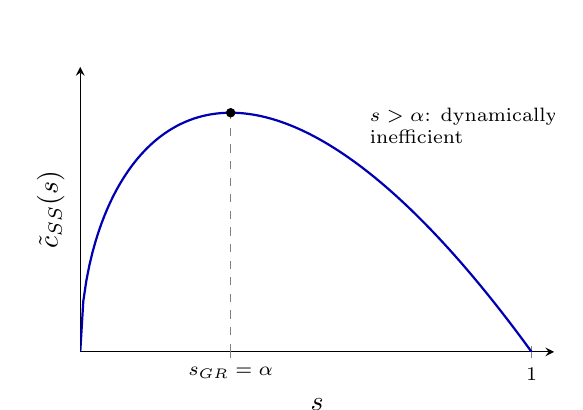
\begin{tikzpicture}
\begin{axis}[width=7.6cm,height=5.2cm,axis lines=left,xmin=0,xmax=1.05,ymin=0,ymax=1.45,
  xlabel={$s$},ylabel={$\tilde c_{SS}(s)$},xtick={0.3333,1},xticklabels={$s_{GR}=\alpha$,$1$},ytick=\empty,
  every tick label/.append style={font=\scriptsize}]
\addplot[domain=0:1,samples=150,thick,blue!70!black]{(1-x)*sqrt(x/0.1)};
\draw[dashed,gray](axis cs:0.3333,0)--(axis cs:0.3333,1.217);
\addplot[only marks,mark=*,mark size=1.5pt]coordinates{(0.3333,1.217)};
\node[font=\scriptsize,anchor=west,align=left] at (axis cs:0.62,1.15){$s>\alpha$: dynamically\\inefficient};
\end{axis}
\end{tikzpicture}\\
{\footnotesize Figure 2. Steady-state consumption per efficiency unit against $s$ (drawn for $\alpha=1/3$, $\xi=0.1$):
zero at $s=0$ (nothing to consume from) and at $s=1$ (nothing consumed), maximum at $s=\alpha$.}
\end{center}
\intuicao{Saving more raises $\tilde k$ and output, but each extra unit of capital also needs $\xi$ of
investment every period just to be kept per efficiency unit. Consumption is maximised when the last unit
of capital produces exactly what it costs to maintain: $f'(\tilde k)=\xi$. Above that point ($s>\alpha$) the
economy could consume more today and forever by saving less.}
\refbib{Kurlat \S4.3, pp.~61--63 (golden rule, $s_{gold}=\alpha$); \S4.5, pp.~69--72.}
\rubrica{
\item $\tilde c_{SS}(s)$ with exponent $\alpha/(1-\alpha)$: 0.3 pt.
\item FOC and $s_{GR}=\alpha$ (SOC or cross-check $f'=\xi$): 0.3 pt.
\item Per-worker consumption at every date maximised: 0.2 pt. Effect of $g$ on $s_{GR}$ and $\tilde k_{GR}$: 0.1 pt.
\item Intuition (marginal product equals break-even cost): 0.1 pt.
\item Exponent dropped in the substitution ($s=1/(2-\alpha)$): max.\ 0.4 pt. Maximising $\tilde k$ (answer $s=1$): max.\ 0.2 pt.
}
\gap{Prova 01, 2.b: the $\sigma$ (here $\alpha$) in the exponent of $c_{SS}$ was dropped.}
\end{sol}

\sub{2.c}{1 point} Consider now the competitive equilibrium of an economy that lasts only two
periods, $t=1,2$. There is an initial capital stock $K_1>0$, which belongs to the representative
firm and depreciates fully once used in period~1. The representative firm maximises profits in
perfectly competitive markets and has production function (1) in both periods, with
$A_2=(1+g)A_1$. The representative consumer owns the firm and receives its profits $\Pi_1$ and
$\Pi_2$. In each period the consumer has one unit of time, which it splits between work $L_t$ and
leisure $1-L_t$, and earns real labour income $w_tA_tL_t$ ($w_t$ is the real wage per efficiency
unit of labour). Income not consumed in period~1 is saved as an asset $a_1$ that pays the real
interest rate $r$; the only asset in this economy is the capital the firm uses in period~2, $K_2$,
which also depreciates fully once used. Intertemporal utility is
\[
U=\ln c_1+\gamma\ln(1-L_1)+\beta\left[\ln c_2+\gamma\ln(1-L_2)\right],\qquad \beta\in(0,1),\ \gamma>0.
\]
Derive and explain the intertemporal budget constraint of this consumer.
\resolespaco[6cm]
\begin{sol}
\begin{notacao}
\item $c_1$, $c_2>0$: consumption in periods 1 and 2. $L_t\in[0,1]$: hours worked; $1-L_t$: leisure
(time endowment normalised to 1).
\item $A_t>0$: technology, with $A_2=(1+g)A_1$. $w_t>0$: real wage per efficiency unit of labour, so
labour income is $w_tA_tL_t$.
\item $\Pi_1$, $\Pi_2$: the firm's profits, paid to the consumer who owns it.
\item $a_1$: asset carried from period 1 to period 2; of either sign for one consumer (in
equilibrium it is the capital $K_2>0$). $r>-1$: real interest rate between the periods.
\item $\beta\in(0,1)$: discount factor. $\gamma>0$: weight of leisure in utility.
\item $H>0$: full lifetime income, the present value of the time endowment plus profits (step 3).
\end{notacao}
\passo{period constraints}{In period 1, uses equal sources:}
\begin{equation}
\boxed{c_1+a_1=w_1A_1L_1+\Pi_1} \label{q2c:b1}
\end{equation}
Period 2 is the last: nothing is left for later, and nobody would lend to a consumer who cannot
repay after period 2. So the consumer spends the asset with its return plus period-2 income:
\begin{equation}
\boxed{c_2=(1+r)a_1+w_2A_2L_2+\Pi_2} \label{q2c:b2}
\end{equation}
Profits appear because the consumer owns the firm; with no initial financial wealth, they are its
only non-labour income besides the return on $a_1$.
\passo{eliminate $a_1$}{Solve \eqref{q2c:b2} for $a_1$:}
\begin{equation}
a_1=\frac{c_2-w_2A_2L_2-\Pi_2}{1+r}. \label{q2c:a1}
\end{equation}
Substitute \eqref{q2c:a1} into \eqref{q2c:b1}:
\[
c_1+\frac{c_2-w_2A_2L_2-\Pi_2}{1+r}=w_1A_1L_1+\Pi_1 .
\]
Move the period-2 income terms to the right side:
\begin{equation}
\boxed{c_1+\frac{c_2}{1+r}=w_1A_1L_1+\Pi_1+\frac{w_2A_2L_2+\Pi_2}{1+r}} \label{q2c:ibc}
\end{equation}
\passo{full-income form}{Value leisure at its opportunity cost, the wage. Add
$w_1A_1(1-L_1)+\frac{w_2A_2(1-L_2)}{1+r}$ to both sides of \eqref{q2c:ibc}; on the right,
$w_tA_tL_t+w_tA_t(1-L_t)=w_tA_t$:}
\begin{align}
&c_1+w_1A_1(1-L_1)+\frac{c_2+w_2A_2(1-L_2)}{1+r}\nonumber\\
&\qquad=\big[w_1A_1L_1+w_1A_1(1-L_1)\big]+\Pi_1+\frac{\big[w_2A_2L_2+w_2A_2(1-L_2)\big]+\Pi_2}{1+r}\nonumber\\
&\qquad=H, \label{q2c:full}
\end{align}
where
\begin{equation}
H\equiv w_1A_1+\Pi_1+\frac{w_2A_2+\Pi_2}{1+r}. \label{q2c:H}
\end{equation}
\passo{reading}{By \eqref{q2c:full}--\eqref{q2c:H}, the \textbf{present value} of lifetime
consumption (and of leisure, priced at the wage) equals the present value of lifetime income: the
value of the whole time endowment plus profits, with period-2 amounts discounted at $1+r$. $a_1$ may
be of either sign for one consumer; it disappears from the lifetime constraint \eqref{q2c:ibc}
because borrowing and lending only move resources across periods at the price $1/(1+r)$. The
constraint binds: $u'>0$, so unspent resources at the end are never optimal.}
\refbib{Kurlat \S6.2, pp.~105--112 (intertemporal budget constraint); \S7.2, pp.~131--137 (time endowment,
labour income); ch.~9, \S9.1 (households own the firms).}
\rubrica{
\item Two period constraints, with $\Pi_1,\Pi_2$ and the labour income of both periods: 0.4 pt.
\item Elimination of $a_1$ to the present-value constraint: 0.3 pt.
\item Explanation as a present-value statement (why $1+r$ discounts, why it binds): 0.3 pt.
\item Profits omitted: $-0.2$. ``Consumption adjusted by $r$'' without the present-value reading: max.\ 0.1 on the last line.
}
\gap{Prova 01, 2.c: firm profits omitted from the budget constraint; reading not stated in present value.}
\end{sol}

\sub{2.d}{1 point} Set up the problem of the consumer of item 2.c and derive the first-order
conditions for \emph{all} of its choice variables, including the equation describing the
intertemporal consumption decision and the consumption--leisure decision in each period. Then find
the equation that gives the optimal $c_1$ as a function only of parameters, prices and levels of
income and wealth, and interpret it economically.
\resolespaco[7cm]
\begin{sol}
\begin{notacao}
\item As in 2.c. New: $\lambda_1$, $\lambda_2>0$, the multipliers on \eqref{q2c:b1} and
\eqref{q2c:b2}: the marginal utility of one more unit of income in period $t$.
\end{notacao}
\passo{problem}{Choice variables: $c_1,c_2,L_1,L_2,a_1$; prices $w_1,w_2,r$ and profits
$\Pi_1,\Pi_2$ are taken as given. Maximise $U$ subject to \eqref{q2c:b1} and \eqref{q2c:b2}, with
one multiplier per period constraint:}
\begin{align}
\mathcal L={}&\ln c_1+\gamma\ln(1-L_1)+\beta\ln c_2+\beta\gamma\ln(1-L_2)\nonumber\\
&+\lambda_1\left[w_1A_1L_1+\Pi_1-c_1-a_1\right]+\lambda_2\left[(1+r)a_1+w_2A_2L_2+\Pi_2-c_2\right]. \label{q2d:lag}
\end{align}
\passo{FOCs}{Differentiate \eqref{q2d:lag} with respect to each choice variable and set the
derivative to zero:}
\begin{align}
c_1:&\quad \frac{1}{c_1}=\lambda_1, \label{q2d:c1}\\
c_2:&\quad \frac{\beta}{c_2}=\lambda_2, \label{q2d:c2}\\
L_1:&\quad \frac{\gamma}{1-L_1}=\lambda_1w_1A_1, \label{q2d:L1}\\
L_2:&\quad \frac{\beta\gamma}{1-L_2}=\lambda_2w_2A_2, \label{q2d:L2}\\
a_1:&\quad \lambda_1=(1+r)\lambda_2. \label{q2d:a1}
\end{align}
Log utility makes every solution interior: as $L_t\to1$ the marginal utility of leisure goes to
infinity, and as $c_t\to0$ that of consumption does.
\passo{Euler (intertemporal)}{Substitute \eqref{q2d:c1} and \eqref{q2d:c2} into \eqref{q2d:a1}:}
\begin{align*}
\left(\frac{1}{c_1}\right) &= (1+r)\left(\frac{\beta}{c_2}\right)\\
\frac{1}{c_1} &= \beta(1+r)\frac{1}{c_2}.
\end{align*}
Multiply by $c_1c_2$:
\begin{equation}
\boxed{c_2=\beta(1+r)\,c_1} \label{q2d:euler}
\end{equation}
The marginal rate of substitution between $c_1$ and $c_2$ equals the relative price $1+r$.
\passo{consumption--leisure (intratemporal)}{Divide \eqref{q2d:L1} by \eqref{q2d:c1}, and
\eqref{q2d:L2} by \eqref{q2d:c2}; the multipliers cancel:}
\begin{align*}
\frac{\gamma/(1-L_1)}{1/c_1} &= \frac{\lambda_1w_1A_1}{\lambda_1},\\
\frac{\beta\gamma/(1-L_2)}{\beta/c_2} &= \frac{\lambda_2w_2A_2}{\lambda_2}.
\end{align*}
\begin{equation}
\boxed{\frac{\gamma c_1}{1-L_1}=w_1A_1} \label{q2d:intra1}
\end{equation}
\begin{equation}
\boxed{\frac{\gamma c_2}{1-L_2}=w_2A_2} \label{q2d:intra2}
\end{equation}
In each period the MRS between leisure and consumption equals the real wage (the price of an hour
of leisure).
\passo{solve for $c_1$}{Express each term on the left of the full-income constraint
\eqref{q2c:full} in terms of $c_1$. From \eqref{q2d:euler}, \eqref{q2d:intra1}, and
\eqref{q2d:intra2} followed by \eqref{q2d:euler}:}
\begin{align}
\frac{c_2}{1+r} &= \frac{\big[\beta(1+r)c_1\big]}{1+r}\nonumber\\
&= \beta c_1, \label{q2d:t1}\\
w_1A_1(1-L_1) &= \gamma c_1, \label{q2d:t2}\\
\frac{w_2A_2(1-L_2)}{1+r} &= \frac{\gamma c_2}{1+r}\nonumber\\
&= \frac{\gamma\big[\beta(1+r)c_1\big]}{1+r}\nonumber\\
&= \beta\gamma c_1. \label{q2d:t3}
\end{align}
Split the fraction in \eqref{q2c:full} and substitute \eqref{q2d:t1}--\eqref{q2d:t3}:
\begin{align*}
c_1+w_1A_1(1-L_1)+\frac{c_2}{1+r}+\frac{w_2A_2(1-L_2)}{1+r} &= H\\
c_1+(\gamma c_1)+(\beta c_1)+(\beta\gamma c_1) &= H\\
c_1(1+\gamma+\beta+\beta\gamma) &= H\\
c_1(1+\beta)(1+\gamma) &= H.
\end{align*}
Divide by $(1+\beta)(1+\gamma)$ and write $H$ out with \eqref{q2c:H}:
\begin{align}
c_1 &= \frac{H}{(1+\beta)(1+\gamma)}\nonumber\\
&= \boxed{\frac{1}{(1+\beta)(1+\gamma)}\left[w_1A_1+\Pi_1+\frac{w_2A_2+\Pi_2}{1+r}\right]} \label{q2d:c1sol}
\end{align}
Then \eqref{q2d:euler}, \eqref{q2d:intra1}--\eqref{q2d:intra2} and \eqref{q2c:b1} give the other
choices:
\begin{align*}
c_2 &= \beta(1+r)\,c_1,\\
1-L_t &= \frac{\gamma c_t}{w_tA_t},\quad t=1,2,\\
a_1 &= w_1A_1L_1+\Pi_1-c_1.
\end{align*}
\passo{interpretation}{By \eqref{q2d:t1}--\eqref{q2d:c1sol}, with log utility the consumer spends fixed shares of full lifetime wealth $H$:
$\frac{1}{(1+\beta)(1+\gamma)}$ on $c_1$, $\frac{\gamma}{(1+\beta)(1+\gamma)}$ on leisure in period 1,
$\frac{\beta}{(1+\beta)(1+\gamma)}$ and $\frac{\beta\gamma}{(1+\beta)(1+\gamma)}$ on period~2.
$c_1$ depends on \emph{lifetime} resources, not on period-1 income alone (permanent income).
$\beta\uparrow\Rightarrow c_1\downarrow$ (patience moves spending to period 2); $\gamma\uparrow\Rightarrow
c_1\downarrow$ for given $H$ (more of full wealth is taken as leisure). Given $H$, $r$ does not enter: for
the shares, the income and substitution effects of $r$ cancel with log utility; $r$ moves $c_1$ only
through the present value of period-2 income in $H$ (a higher $r$ lowers it, so $c_1$ falls).}
\intuicao{Contrast with Prova 01: there work had no utility cost, so $L_1=1$ was a corner and saying so
was the FOC. Here leisure is valued, so hours are an interior choice and the wage is the price of leisure.}
\refbib{Kurlat \S6.2, pp.~105--115 (Euler equation, log closed forms); \S7.2, pp.~131--137 (consumption--leisure);
ch.~9, \S9.1, eq.~(9.1.7)--(9.1.8).}
\rubrica{
\item Problem stated with all five choice variables: 0.1 pt.
\item FOCs for $c_1,c_2$ and the Euler equation: 0.3 pt. FOCs for $L_1$ and $L_2$ (intratemporal conditions): 0.2 pt (0.1 each).
\item FOC for $a_1$ (or the substitution that eliminates it): 0.1 pt.
\item $c_1$ in closed form: 0.2 pt. Interpretation ($H$, $\beta$, $\gamma$, role of $r$): 0.1 pt.
\item No FOC for hours: max.\ 0.6 pt. Substitution route instead of Lagrangian: full credit.
}
\gap{Prova 01, 2.d: FOC for $L_1$ missing (``todas as variáveis de sua escolha'').}
\end{sol}

\sub{2.e}{1 point} Calculate the saving rate of this representative consumer (the share of saving
in the consumer's period-1 income), recalling that markets are perfectly competitive. Find the hours
worked in each period. Then find an expression for $\hat k_2\equiv K_2/A_2$ as a function only of
$\hat k_1\equiv K_1/A_1$ and of parameters. Treating this expression as a law of motion that applies
period after period, draw it with $\hat k_1$ on the horizontal axis and $\hat k_2$ on the vertical
axis, and show graphically the steady state of this economy. Is it stable? Justify.
\resolespaco[8cm]
\begin{sol}
\begin{notacao}
\item As in 2.c--2.d. New: $Y_1$, $Y_2>0$, output in each period by \eqref{q2:Y}; $K_2>0$, the
capital built from period-1 saving.
\item $s^\ast\in(0,1)$: the consumer's saving rate. $\hat k_t\equiv K_t/A_t>0$: capital per unit of
technology.
\item $\phi(\hat k)$: the law of motion $\hat k_{t+1}=\phi(\hat k_t)$. $\hat k_{SS}$: its fixed point.
$\hat k_{GR}$ (Figure 3): the fixed point of the same map with $s=s_{GR}$.
\end{notacao}
\passo{firm, period 1}{The firm owns $K_1$ and hires labour:}
\begin{equation}
\max_{L_1}\ K_1^{\alpha}(A_1L_1)^{1-\alpha}-w_1A_1L_1. \label{q2e:firm1}
\end{equation}
The FOC of \eqref{q2e:firm1}, with $Y_1$ from \eqref{q2:Y}:
\begin{equation}
(1-\alpha)\frac{Y_1}{L_1}=w_1A_1. \label{q2e:foc1}
\end{equation}
Multiply \eqref{q2e:foc1} by $L_1$ to get the wage bill:
\begin{equation}
w_1A_1L_1=(1-\alpha)Y_1. \label{q2e:wb1}
\end{equation}
Profit is output minus the wage bill \eqref{q2e:wb1}:
\begin{align}
\Pi_1 &= Y_1-w_1A_1L_1\nonumber\\
&= Y_1-(1-\alpha)Y_1\nonumber\\
&= \boxed{\alpha Y_1}, \label{q2e:pi1}
\end{align}
the return on the capital the firm owns, paid to its owner.
\passo{firm, period 2}{The firm borrows $K_2$ from the consumer and repays $(1+r)K_2$ (the capital
is used up):}
\begin{equation}
\max_{K_2,L_2}\ K_2^{\alpha}(A_2L_2)^{1-\alpha}-w_2A_2L_2-(1+r)K_2. \label{q2e:firm2}
\end{equation}
The FOCs of \eqref{q2e:firm2}:
\begin{align}
\alpha\frac{Y_2}{K_2} &= 1+r, \label{q2e:r}\\
(1-\alpha)\frac{Y_2}{L_2} &= w_2A_2. \label{q2e:w2}
\end{align}
Multiply \eqref{q2e:r} by $K_2$ and \eqref{q2e:w2} by $L_2$ and subtract both payments from output.
With constant returns:
\begin{align}
\Pi_2 &= Y_2-w_2A_2L_2-(1+r)K_2\nonumber\\
&= Y_2-(1-\alpha)Y_2-\alpha Y_2\nonumber\\
&= \boxed{0}. \label{q2e:pi2}
\end{align}
\passo{market clearing}{The only asset is the capital of period 2, so the asset market clears when}
\begin{equation}
\boxed{a_1=K_2} \label{q2e:mc}
\end{equation}
The goods markets clear when
\begin{align}
c_1+K_2 &= Y_1, \label{q2e:g1}\\
c_2 &= Y_2. \label{q2e:g2}
\end{align}
Labour: $L_t$ supplied $=$ $L_t$ demanded. Check: by \eqref{q2e:r}, \eqref{q2e:w2} and
\eqref{q2e:pi2}, period-2 income in \eqref{q2c:b2} is
\[
(1+r)K_2+w_2A_2L_2+\Pi_2=\alpha Y_2+(1-\alpha)Y_2+0=Y_2 .
\]
\passo{saving rate}{Substitute \eqref{q2e:g2} and \eqref{q2e:r} into the Euler equation
\eqref{q2d:euler}, then multiply by $K_2/Y_2$:}
\begin{align}
(Y_2) &= \beta\left(\frac{\alpha Y_2}{K_2}\right)c_1\nonumber\\
K_2 &= \alpha\beta\,c_1. \label{q2e:K2c1}
\end{align}
Substitute \eqref{q2e:K2c1} into the period-1 goods market \eqref{q2e:g1}:
\begin{align}
c_1+(\alpha\beta c_1) &= Y_1\nonumber\\
c_1 &= \frac{Y_1}{1+\alpha\beta}. \label{q2e:c1}
\end{align}
Substitute \eqref{q2e:c1} into \eqref{q2e:K2c1} and use \eqref{q2e:mc}:
\begin{align}
K_2 &= \alpha\beta\left(\frac{Y_1}{1+\alpha\beta}\right)\nonumber\\
a_1=K_2 &= \frac{\alpha\beta}{1+\alpha\beta}\,Y_1. \label{q2e:a1}
\end{align}
Period-1 income, by \eqref{q2e:wb1} and \eqref{q2e:pi1}:
\begin{align}
w_1A_1L_1+\Pi_1 &= (1-\alpha)Y_1+\alpha Y_1\nonumber\\
&= Y_1. \label{q2e:inc1}
\end{align}
Divide \eqref{q2e:a1} by \eqref{q2e:inc1}:
\begin{align}
s^\ast &= \frac{a_1}{w_1A_1L_1+\Pi_1}\nonumber\\
&= \frac{\left(\frac{\alpha\beta}{1+\alpha\beta}\,Y_1\right)}{(Y_1)}\nonumber\\
&= \boxed{\frac{\alpha\beta}{1+\alpha\beta}}\quad\text{(constant: no }K_1,A_1,g,\gamma\text{)}. \label{q2e:s}
\end{align}
\passo{hours}{Period 2: substitute \eqref{q2e:g2} for $c_2$ and \eqref{q2e:w2} for $w_2A_2$ into
\eqref{q2d:intra2}:}
\begin{align}
\frac{\gamma(Y_2)}{1-L_2} &= \left(\frac{(1-\alpha)Y_2}{L_2}\right)\nonumber\\
\gamma L_2 &= (1-\alpha)(1-L_2)\nonumber\\
L_2(1-\alpha+\gamma) &= 1-\alpha\nonumber\\
L_2 &= \boxed{\frac{1-\alpha}{1-\alpha+\gamma}}. \label{q2e:L2}
\end{align}
Period 1: substitute \eqref{q2e:c1} for $c_1$ and \eqref{q2e:foc1} for $w_1A_1$ into
\eqref{q2d:intra1}:
\begin{align}
\frac{\gamma\left(\frac{Y_1}{1+\alpha\beta}\right)}{1-L_1} &= \left(\frac{(1-\alpha)Y_1}{L_1}\right)\nonumber\\
\frac{\gamma Y_1}{(1+\alpha\beta)(1-L_1)} &= \frac{(1-\alpha)Y_1}{L_1}\nonumber\\
\gamma L_1 &= (1-\alpha)(1+\alpha\beta)(1-L_1)\nonumber\\
L_1\big[(1-\alpha)(1+\alpha\beta)+\gamma\big] &= (1-\alpha)(1+\alpha\beta)\nonumber\\
L_1 &= \boxed{\frac{(1-\alpha)(1+\alpha\beta)}{(1-\alpha)(1+\alpha\beta)+\gamma}}. \label{q2e:L1}
\end{align}
Neither \eqref{q2e:L2} nor \eqref{q2e:L1} depends on $K_1$ or $A_t$: with log utility the income and
substitution effects of a higher wage cancel. $L_1>L_2$: in period 1 consumption is only the share
$1/(1+\alpha\beta)$ of output, so a unit of income is worth more at the margin (part of it is saved)
and the consumer works more.
\passo{law of motion}{By \eqref{q2e:a1}, \eqref{q2e:s} and \eqref{q2:Y}:}
\begin{align}
K_2 &= s^\ast Y_1\nonumber\\
&= s^\ast K_1^{\alpha}(A_1L_1)^{1-\alpha}. \label{q2e:K2}
\end{align}
Divide \eqref{q2e:K2} by $A_2=(1+g)A_1$ and use $K_1=\hat k_1A_1$:
\begin{align}
\hat k_2 &= \frac{s^\ast(\hat k_1A_1)^{\alpha}(A_1L_1)^{1-\alpha}}{(1+g)A_1}\nonumber\\
&= \frac{s^\ast A_1\,\hat k_1^{\alpha}L_1^{1-\alpha}}{(1+g)A_1}\nonumber\\
&= \boxed{\frac{s^\ast L_1^{1-\alpha}}{1+g}\,\hat k_1^{\alpha}}\equiv\phi(\hat k_1). \label{q2e:phi}
\end{align}
\passo{steady state and stability}{From \eqref{q2e:phi}: $\phi(0)=0$, $\phi'>0$, $\phi''<0$,
$\phi'\to\infty$ as $\hat k\to0$ and $\phi'\to0$ as $\hat k\to\infty$. The curve starts above the
45-degree line and ends below it, so it crosses it exactly once at a positive point. Set
$\hat k=\phi(\hat k)$ in \eqref{q2e:phi}:}
\begin{align*}
\hat k &= \frac{s^\ast L_1^{1-\alpha}}{1+g}\,\hat k^{\alpha}\\
\hat k^{1-\alpha} &= \frac{s^\ast L_1^{1-\alpha}}{1+g}.
\end{align*}
Raise both sides to the power $1/(1-\alpha)$:
\begin{equation}
\boxed{\hat k_{SS}=\left(\frac{s^\ast L_1^{1-\alpha}}{1+g}\right)^{\frac{1}{1-\alpha}}} \label{q2e:kss}
\end{equation}
Differentiate \eqref{q2e:phi}:
\begin{align*}
\phi'(\hat k) &= \alpha\,\frac{s^\ast L_1^{1-\alpha}}{1+g}\,\hat k^{\alpha-1}\\
&= \alpha\,\frac{\phi(\hat k)}{\hat k}.
\end{align*}
At the fixed point $\phi(\hat k_{SS})=\hat k_{SS}$, so
\begin{align*}
\phi'(\hat k_{SS}) &= \alpha\,\frac{\phi(\hat k_{SS})}{\hat k_{SS}}\\
&= \alpha\,\frac{(\hat k_{SS})}{\hat k_{SS}}\\
&= \alpha<1\ \Rightarrow\ \text{stable}.
\end{align*}
From any $\hat k_1<\hat k_{SS}$ the staircase between $\phi$ and the 45-degree line climbs
monotonically to $\hat k_{SS}$ (Figure 3).
\begin{center}
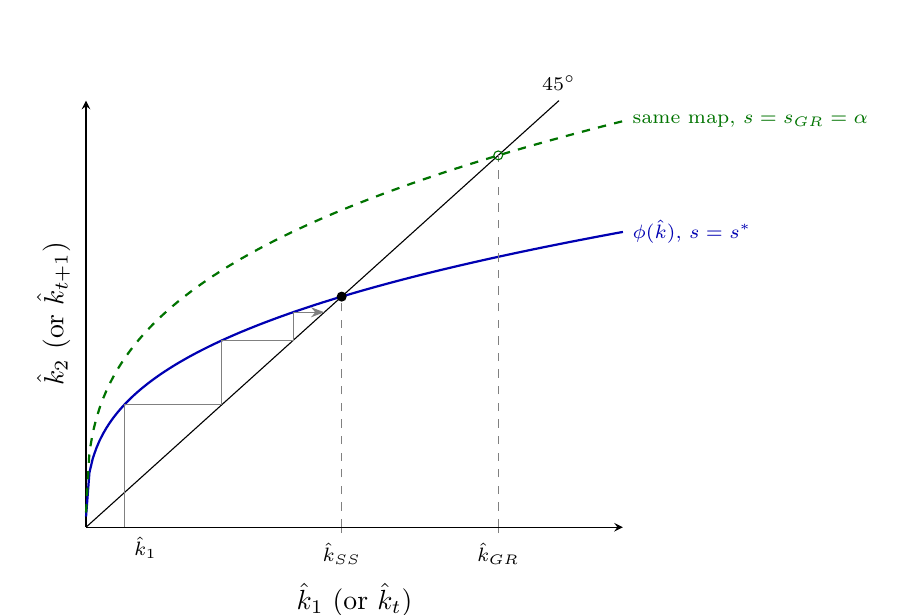
\begin{tikzpicture}
\begin{axis}[width=8.4cm,height=7cm,axis lines=left,xmin=0,xmax=2.1,ymin=0,ymax=1.85,clip=false,
  xlabel={$\hat k_1$ (or $\hat k_t$)},ylabel={$\hat k_2$ (or $\hat k_{t+1}$)},xtick={1,1.6124},
  xticklabels={$\hat k_{SS}$,$\hat k_{GR}$},ytick=\empty,every tick label/.append style={font=\scriptsize}]
\addplot[domain=0:1.85,thin,black]{x};
\addplot[domain=0.0001:2.1,samples=160,thick,blue!70!black]{x^(1/3)};
\addplot[domain=0.0001:2.1,samples=160,thick,dashed,green!45!black]{1.375*x^(1/3)};
\node[font=\scriptsize,anchor=south] at (axis cs:1.85,1.85){$45^\circ$};
\node[font=\scriptsize,blue!70!black,anchor=west] at (axis cs:2.1,1.281){$\phi(\hat k)$, $s=s^\ast$};
\node[font=\scriptsize,green!45!black,anchor=west] at (axis cs:2.1,1.761){same map, $s=s_{GR}=\alpha$};
\draw[gray,-{Stealth}](axis cs:0.15,0)--(axis cs:0.15,0.5313)--(axis cs:0.5313,0.5313)--(axis cs:0.5313,0.8099)
  --(axis cs:0.8099,0.8099)--(axis cs:0.8099,0.9321)--(axis cs:0.9321,0.9321);
\addplot[only marks,mark=*,mark size=1.6pt]coordinates{(1,1)};
\addplot[only marks,mark=o,mark size=1.6pt,green!45!black]coordinates{(1.6124,1.6124)};
\draw[dashed,gray](axis cs:1,0)--(axis cs:1,1);
\draw[dashed,gray](axis cs:1.6124,0)--(axis cs:1.6124,1.6124);
\node[font=\scriptsize,anchor=north west] at (axis cs:0.15,0){$\hat k_1$};
\end{axis}
\end{tikzpicture}\\
{\footnotesize Figure 3. The equilibrium law of motion (solid) crosses the 45-degree line once; the staircase
from a low $\hat k_1$ converges to $\hat k_{SS}$. Dashed: the same map with $s=\alpha$, whose fixed point is the
golden rule (used in 2.f). Drawn for $\alpha=1/3$, $\beta=0.96$, units chosen so that $\hat k_{SS}=1$.}
\end{center}
\intuicao{Patience and the productivity of capital set the saving rate; diminishing returns ($\alpha<1$) make
each extra unit of capital produce less, so saving a fixed share of a concave output cannot sustain unbounded
growth of $\hat k$.}
\refbib{Kurlat ch.~9, \S9.1 (firm FOCs, market clearing, $r=r^K-\delta$ with $\delta=1$); \S4.4, pp.~63--69
(factor shares, zero profit under constant returns); \S4.2, pp.~59--61 (stability).}
\rubrica{
\item Firm FOCs, $\Pi_1=\alpha Y_1$, $\Pi_2=0$, $1+r=\alpha Y_2/K_2$: 0.2 pt.
\item Market clearing $a_1=K_2$ (and goods): 0.1 pt. Saving rate $\alpha\beta/(1+\alpha\beta)$ derived: 0.2 pt.
\item Hours $L_1$, $L_2$: 0.1 pt. Map $\hat k_2(\hat k_1)$: 0.2 pt.
\item Diagram: axes, 45-degree line, concave map from the origin, $\hat k_{SS}$ at the crossing, stability argued: 0.2 pt.
\item Saving rate quoted from Solow's $s$ or left as a function of prices: 0 for that line. No market clearing ($K_2\neq a_1$): max.\ 0.5 pt. A map that does not cross the 45-degree line: 0 for the diagram.
}
\gap{Prova 01, 2.e: saving rate not derived; no market clearing $K_2=a_1$; diagram without a valid steady state.}
\end{sol}

\sub{2.f}{0.5 point} Discuss intuitively the relation between the model of items 2.c--2.e and the
Solow model of items 2.a--2.b. In particular, compare the saving rate found in 2.e with $s_{GR}$ and
explain the difference.
\resolespaco[5cm]
\begin{sol}
\begin{notacao}
\item As in 2.a--2.e. New: $\tilde k_t\equiv\hat k_t/L_1=K_t/(A_tL_1)>0$, capital per efficiency unit
of \emph{hours} (in 2.a, per efficiency unit of workers).
\end{notacao}
\passo{same law of motion}{Write \eqref{q2e:phi}, applied period after period, in terms of
$\tilde k_t=\hat k_t/L_1$:}
\begin{align}
L_1\tilde k_{t+1} &= \frac{s^\ast L_1^{1-\alpha}}{1+g}\,(L_1\tilde k_t)^{\alpha}\nonumber\\
&= \frac{s^\ast L_1}{1+g}\,\tilde k_t^{\alpha}\nonumber\\
(1+g)\tilde k_{t+1} &= s^\ast\tilde k_t^{\alpha}. \label{q2f:lom}
\end{align}
Set $\boxed{\delta=1}$ (capital used up in one period) and $\boxed{n=0}$ (one consumer) in the
Solow law of motion \eqref{q2a:lom}, which is equation \eqref{q2:K} divided as in 2.a:
\begin{align}
\tilde k_{t+1} &= \frac{(1-1)\tilde k_t+s\tilde k_t^{\alpha}}{(1+g)(1+0)}\nonumber\\
&= \frac{s\tilde k_t^{\alpha}}{1+g}\nonumber\\
(1+g)\tilde k_{t+1} &= s\,\tilde k_t^{\alpha}. \label{q2f:solow}
\end{align}
\eqref{q2f:lom} is \eqref{q2f:solow} with $s=s^\ast$. Indeed, by \eqref{q2e:kss},
\begin{align*}
\hat k_{SS} &= \left(\frac{s^\ast L_1^{1-\alpha}}{1+g}\right)^{\frac{1}{1-\alpha}}\\
&= L_1\left(\frac{s^\ast}{1+g}\right)^{\frac{1}{1-\alpha}}\\
&= L_1\left(\frac{s^\ast}{(1+g)(1+0)-(1-1)}\right)^{\frac{1}{1-\alpha}},
\end{align*}
which is 2.a's $\tilde k_{SS}$ \eqref{q2a:kss} times the hours worked.
\passo{what is new}{Solow \emph{assumes} $s$ and the labour input. Here both are \emph{chosen}:
$s^\ast=\alpha\beta/(1+\alpha\beta)$ in \eqref{q2e:s} comes from patience $\beta$ and the return to
capital $\alpha$, and log utility makes it constant (independent of $K$, $A$, $g$) --- a
microfoundation for Solow's constant saving rate. Hours $L_1$ in \eqref{q2e:L1} depend on the taste
for leisure $\gamma$ and on $\beta$.}
\passo{against the golden rule}{Compare \eqref{q2e:s} with $s_{GR}=\alpha$ from \eqref{q2b:sgr}:}
\begin{align*}
s^\ast<\alpha &\iff \frac{\alpha\beta}{1+\alpha\beta}<\alpha\\
&\iff \frac{\beta}{1+\alpha\beta}<1\\
&\iff \beta<1+\alpha\beta\\
&\iff \beta(1-\alpha)<1,
\end{align*}
always true, since $\beta<1$ and $1-\alpha<1$. So $\boxed{s^\ast<\alpha}$ and $\hat k_{SS}<\hat k_{GR}$
(Figure 3): the competitive economy accumulates \emph{less} than the golden rule. Even as
$\beta\to1$, $s^\ast\to\alpha/(1+\alpha)<\alpha$: here saving finances one period of consumption
only, since the horizon ends.
\passo{why this is not a failure}{The golden rule maximises steady-state consumption and ignores that
consumption earlier is worth more to an impatient consumer ($\beta<1$) and that reaching more capital costs
consumption on the way. Markets here are complete and competitive, with no externalities: by the first welfare
theorem the equilibrium is Pareto efficient, and it is below the golden rule, i.e.\ dynamically efficient. The
golden rule is a property of steady states, not a welfare criterion.}
\refbib{Kurlat \S4.3, pp.~61--63; ch.~9, \S9.2 (first welfare theorem) and \S9.3 (comparison with the golden rule).}
\rubrica{
\item Same law of motion with $\delta=1$, $n=0$: 0.1 pt.
\item Saving (and hours) chosen, not assumed, and from which primitives: 0.2 pt.
\item $s^\ast<\alpha$ shown, with the reason (impatience; golden rule not a welfare criterion): 0.2 pt.
\item ``It is Solow with $\delta=1$ and $n=0$'' and nothing else: max.\ 0.1 pt.
}
\gap{Prova 01, 2.f: the endogenous saving rate and its comparison with $s_{GR}$ were missing.}
\end{sol}

% =============================================================================
\questao{3}{3}{Consider the simplified New Keynesian model of Benigno (2015), based on the aggregate
demand and supply equations below (barred variables are long-run values, when all firms reset their
prices; the others are short-run values):
\begin{align}
y &= \bar y+(g-\bar g)-\sigma\left[i-(\bar p-p)\right]-\sigma\ln\beta, \tag{AD}\label{q3:AD}\\
p-p^e &= \kappa\,(y-y_n), \tag{AS}\label{q3:AS}
\end{align}
where $p^e$ is the price set by the firms that cannot reset prices and $y_n$ is short-run natural output,
\begin{equation}
y_n=\frac{1+\eta}{\sigma^{-1}+\eta}\,a+\frac{\sigma^{-1}}{\sigma^{-1}+\eta}\,g-\frac{1}{\sigma^{-1}+\eta}\,\mu , \tag{YN}\label{q3:YN}
\end{equation}
$\mu$ being the mark-up; $\bar y$ is given by the same expression evaluated at the long-run values
$\bar a$, $\bar g$, $\bar\mu$; and $y_e=\frac{1+\eta}{\sigma^{-1}+\eta}a+\frac{\sigma^{-1}}{\sigma^{-1}+\eta}g$ is the
efficient level of output. All variables are log deviations from an efficient steady state. Initially
$a=\bar a=g=\bar g=\mu=\bar\mu=0$, $\bar p=p^e$, and the central bank sets $i=\rho\equiv-\ln\beta$, so that
$y=y_n=y_e=\bar y$ and $p=p^e$.}

\sub{3.a}{1 point} News arrives that productivity will be permanently higher in the long run: $\bar a$
rises by $d\bar a>0$, while current productivity $a$ does not change. With $i$ unchanged, represent
graphically, explaining economically why, the initial equilibrium and the shift that defines the new
equilibrium. Compute $dy$ and $dp$. Indicate the gap $y-y_n$ and the gap $y-y_e$ and use both in your
explanation. Is this boom good for welfare today? Justify.
\resolespaco[7cm]
\begin{sol}
\begin{notacao}
\item $y$, $p$: output and price level today; $\bar y$, $\bar p$: their long-run values, when all
firms have reset prices. All are log deviations from the efficient steady state.
\item $p^e$: the price preset by the firms that cannot reset this period.
\item $i$: nominal interest rate, the central bank's instrument. $\beta\in(0,1)$: discount factor;
$\rho\equiv-\ln\beta>0$: the initial (neutral) rate.
\item $a$, $\bar a$: productivity today and in the long run. $g$, $\bar g$: government spending.
$\mu$, $\bar\mu$: the firms' mark-up. All start at 0.
\item $\sigma>0$: intertemporal elasticity of substitution. $\eta>0$: inverse Frisch elasticity of
labour supply. $\kappa>0$: slope of AS.
\item $y_n$: natural output (flexible prices, with the mark-up). $y_e$: efficient output (no mark-up).
\item $\Gamma\equiv\frac{1+\eta}{\sigma^{-1}+\eta}>0$: response of $y_n$, $y_e$ and $\bar y$ to
productivity.
\end{notacao}
\passo{0, the remaining statement equations}{With $\Gamma$ as defined above, the statement gives
long-run output (the expression \eqref{q3:YN} at long-run values) and efficient output:}
\begin{align}
\bar y &= \Gamma\,\bar a+\frac{\sigma^{-1}}{\sigma^{-1}+\eta}\,\bar g-\frac{1}{\sigma^{-1}+\eta}\,\bar\mu, \label{q3:ybar}\\
y_e &= \Gamma\,a+\frac{\sigma^{-1}}{\sigma^{-1}+\eta}\,g. \label{q3:ye}
\end{align}
Substitute $\rho=-\ln\beta$ into \eqref{q3:AD}, then use the initial values $g=\bar g=0$ and
$\bar p=p^e$:
\begin{align}
y &= \bar y+(g-\bar g)-\sigma\left[i-(\bar p-p)\right]-\sigma(-\rho)\nonumber\\
&= \bar y+(g-\bar g)-\sigma(i-\rho)-\sigma(p-\bar p)\nonumber\\
&= \bar y+(0-0)-\sigma(i-\rho)-\sigma\big(p-(p^e)\big)\nonumber\\
&= \bar y-\sigma(i-\rho)-\sigma(p-p^e). \label{q3:ADr}
\end{align}
\passo{which bar moves which curve}{Differentiate \eqref{q3:ybar} with only $\bar a$ moving:}
\begin{equation}
d\bar y=\Gamma\,d\bar a>0. \label{q3a:dybar}
\end{equation}
$\bar y$ is in AD \eqref{q3:ADr}, so \boxed{\text{AD shifts right}} by $\Gamma d\bar a$ at every
$p$ (up by $\Gamma d\bar a/\sigma$). $y_n$ in \eqref{q3:YN} and $y_e$ in \eqref{q3:ye} depend on the
\emph{current} $a$, $g$, $\mu$, none of which moved: \boxed{\text{AS does not move}} (it still passes
through $(y_n,p^e)$), and $y_e=y_n=0$ still.
\passo{why AD moves (Euler)}{Long-run consumption $\bar c=\bar y$ rises: households expect higher permanent
income and, to smooth consumption, want to consume more \emph{today} at the same real rate
$i-(\bar p-p)$. Current demand for goods rises at every price level.}
\passo{new equilibrium}{With $i=\rho$, \eqref{q3:ADr} and \eqref{q3a:dybar} give AD; with $y_n=0$,
\eqref{q3:AS} gives AS:}
\begin{align}
y &= (\Gamma\,d\bar a)-\sigma(\rho-\rho)-\sigma(p-p^e)\nonumber\\
&= \Gamma\,d\bar a-\sigma(p-p^e), \label{q3a:AD}\\
p-p^e &= \kappa\,(y-0)\nonumber\\
&= \kappa\,y. \label{q3a:AS}
\end{align}
Substitute \eqref{q3a:AS} into \eqref{q3a:AD}:
\begin{align*}
y &= \Gamma\,d\bar a-\sigma(\kappa\,y)\\
y(1+\sigma\kappa) &= \Gamma\,d\bar a.
\end{align*}
Divide by $1+\sigma\kappa$ (the initial $y$ is 0, so $y=dy$):
\begin{equation}
\boxed{dy=\frac{\Gamma\,d\bar a}{1+\sigma\kappa}>0} \label{q3a:dy}
\end{equation}
Substitute \eqref{q3a:dy} into \eqref{q3a:AS}:
\begin{align}
dp &= \kappa\,dy\nonumber\\
&= \kappa\left(\frac{\Gamma\,d\bar a}{1+\sigma\kappa}\right)\nonumber\\
&= \boxed{\frac{\kappa\,\Gamma\,d\bar a}{1+\sigma\kappa}>0}. \label{q3a:dp}
\end{align}
\passo{the two gaps}{Since $y_n=y_e=0$, both gaps equal \eqref{q3a:dy}. $y-y_n=dy>0$: output above
natural, which is why prices rise in \eqref{q3a:dp} (AS: flexible-price firms face higher real
marginal cost, because households must be paid a higher real wage to work more). $y-y_e=dy>0$:
output above the efficient level as well.
Chain: $\bar a\uparrow\to\bar y\uparrow\to c\uparrow$ (Euler) $\to$ AD right $\to y>y_n\to$ marginal cost $\uparrow\to$
flexible firms raise $p$ $\to$ real rate $i-(\bar p-p)\uparrow$, which limits the rise in $y$ (movement along AD).
Firms with preset prices keep $p^e$ and produce whatever is demanded.}
\passo{welfare}{\textbf{No.} Today's technology is unchanged, so the efficient output today is unchanged.
The extra output is produced by working beyond the point where the MRS between leisure and consumption equals
today's productivity, and the price surprise $p>p^e$ creates price dispersion across identical firms. Both
terms of the welfare loss are positive: the economy is overheating on a forecast.}
\begin{center}
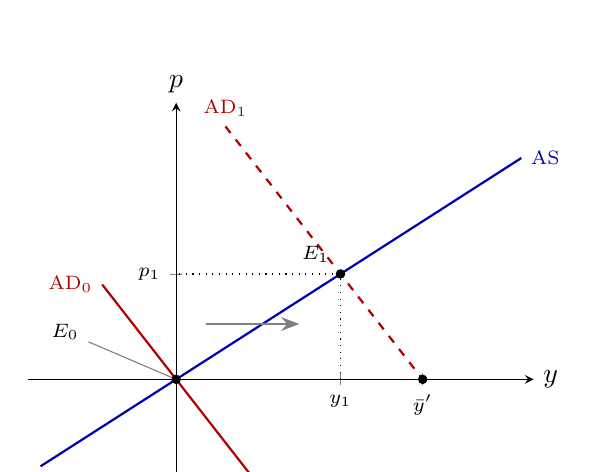
\begin{tikzpicture}
\begin{axis}[width=8cm,height=6.4cm,axis lines=middle,xmin=-0.6,xmax=1.45,ymin=-0.65,ymax=1.75,clip=false,
  xlabel={$y$},ylabel={$p$},xtick={0.6667,1},xticklabels={$y_1$,$\bar y'$},ytick={0.6667},yticklabels={$p_1$},
  every tick label/.append style={font=\scriptsize},x label style={anchor=west},y label style={anchor=south}]
\addplot[thick,blue!70!black,domain=-0.55:1.4]{x};
\addplot[thick,red!70!black,domain=-0.3:0.3]{-2*x};
\addplot[thick,red!70!black,dashed,domain=0.2:1.0]{2-2*x};
\node[font=\scriptsize,blue!70!black,anchor=west] at (axis cs:1.4,1.4){AS};
\node[font=\scriptsize,red!70!black,anchor=east] at (axis cs:-0.3,0.6){AD$_0$};
\node[font=\scriptsize,red!70!black,anchor=south] at (axis cs:0.2,1.6){AD$_1$};
\addplot[only marks,mark=*,mark size=1.5pt]coordinates{(0,0)(0.6667,0.6667)(1,0)};
\node[font=\scriptsize] (e0) at (axis cs:-0.45,0.3){$E_0$};
\draw[gray,thin](e0)--(axis cs:0,0);
\node[font=\scriptsize,anchor=south east] at (axis cs:0.66,0.68){$E_1$};
\draw[dotted](axis cs:0.6667,0)--(axis cs:0.6667,0.6667)--(axis cs:0,0.6667);
\draw[-{Stealth},thick,gray](axis cs:0.12,0.35)--(axis cs:0.5,0.35);
\end{axis}
\end{tikzpicture}\\
{\footnotesize Figure 4. News of higher $\bar a$ shifts AD right (it now passes through $(\bar y',\bar p)$ at $i=\rho$);
AS stays. $E_1$: $y_1-y_n=y_1-y_e>0$ and $p_1>p^e$. (Drawn for $\sigma=0.5$, $\kappa=1$, $\Gamma d\bar a=1$; the origin is
$(y_n,p^e)$.)}
\end{center}
\intuicao{Expectations about the future move demand today. Supply today has not changed, so the extra demand
can only be met by working harder with the same technology, and prices rise.}
\refbib{Benigno (2015) \S6.3, Fig.~8, pp.~511--513; \S5, eqs.~(20)--(21), pp.~509--511; \S4.2--\S4.4 ($y_n$, $y_e$), pp.~508--509.}
\rubrica{
\item AD shifts right, with the Euler/permanent-income reason: 0.3 pt.
\item AS does not move, because $y_n$ depends on current $a,\mu$ only: 0.2 pt.
\item $dy$ and $dp$: 0.2 pt.
\item Both gaps signed and used in the explanation: 0.2 pt. Welfare verdict with the reason: 0.1 pt.
\item Graph lines are inside the first two items (axes $y,p$; AD$_0$, AD$_1$, AS named; $E_0$, $E_1$; direction of the shift).
\item Shifting AS (treating the news as current productivity): max.\ 0.3 pt. Signs of $dy$, $dp$ inconsistent with the graph: $-0.2$.
}
\end{sol}

\sub{3.b}{1 point} Based on the previous item, explain intuitively what a monetary authority committed
to price stability should do after the news, by how much it must move its instrument, and what is the
economic cost of doing so. Show graphically the paths of $y$ and $p$ in the short and in the long run,
with and without that response. A commentator claims that ``whatever the central bank does, it must
give up either price stability or a closed output gap''. Evaluate the claim.
\resolespaco[7cm]
\begin{sol}
\begin{notacao}
\item As in 3.a. New: $r_n$, the natural real interest rate, the real rate that clears today's goods
market at natural output.
\end{notacao}
\passo{target}{Price stability: $p=p^e$. On AS \eqref{q3:AS} this requires $y=y_n$, and since
$y_n=y_e$ here, it also gives $y=y_e$.}
\passo{instrument}{AD must pass through $(y_n,p^e)=(0,p^e)$. Set $y=0$ and $p=p^e$ in \eqref{q3:ADr},
with $\bar y=\Gamma d\bar a$ from \eqref{q3a:dybar}:}
\begin{align*}
0 &= (\Gamma\,d\bar a)-\sigma(i-\rho)-\sigma(p^e-p^e)\\
0 &= \Gamma\,d\bar a-\sigma(i-\rho)\\
\sigma(i-\rho) &= \Gamma\,d\bar a.
\end{align*}
Divide by $\sigma$:
\begin{equation}
\boxed{i=\rho+\frac{\Gamma\,d\bar a}{\sigma}} \label{q3b:i}
\end{equation}
\textbf{Raise} $i$ by $\Gamma d\bar a/\sigma>0$. The natural real rate is
\begin{equation}
r_n=\rho+\sigma^{-1}(\bar y-y_n). \label{q3b:rn}
\end{equation}
Differentiate \eqref{q3b:rn} and substitute \eqref{q3a:dybar} and $dy_n=0$:
\begin{align*}
dr_n &= \sigma^{-1}\big[(\Gamma\,d\bar a)-(0)\big]\\
&= \frac{\Gamma\,d\bar a}{\sigma}.
\end{align*}
The rise in \eqref{q3b:i} is exactly the rise in $r_n$. The future is richer, so the real rate that clears today's goods market
at natural output is higher. AD returns to AD$_0$ in Figure 4.
\passo{cost}{\textbf{None} in terms of the two objectives: after the rise $y=y_n=y_e$ and $p=p^e$. The shock is
\emph{efficient}: it does not separate $y_n$ from $y_e$ (no mark-up moved), so one instrument closes both gaps
(divine coincidence). The commentator is wrong for this shock. A cut, the instinct to ``support the good
news'', would push output and prices further up.}
\passo{long run}{In period 2 all prices adjust and $y=\bar y'=\Gamma d\bar a$, $p=\bar p$, with or without the
response. The higher rate does not cancel the gain; it \emph{times} it: households wait for the productivity to
arrive instead of working beyond the efficient level today. The same response is right if the news is only
optimism; the model cannot tell the two apart in the short run.}
\begin{center}
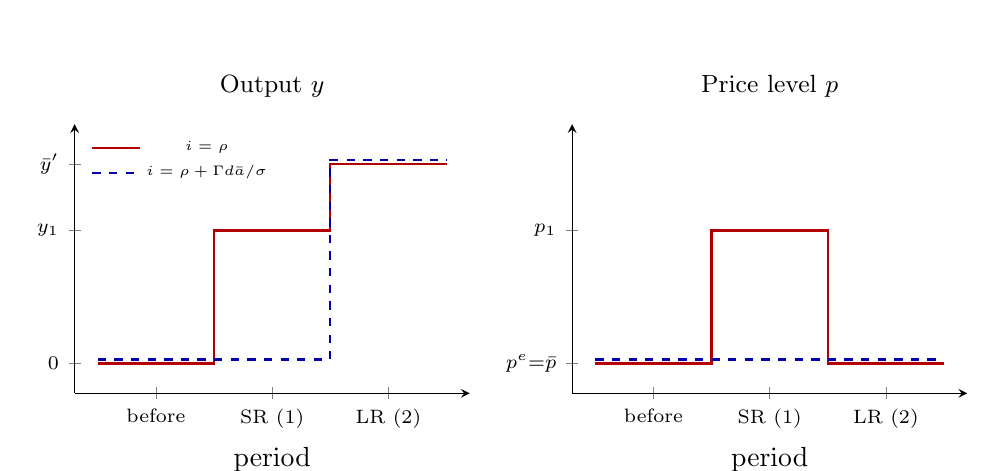
\begin{tikzpicture}
\begin{axis}[name=py,width=6.6cm,height=5cm,axis lines=left,xmin=-0.2,xmax=3.2,ymin=-0.15,ymax=1.2,
  xlabel={period},xtick={0.5,1.5,2.5},xticklabels={before,SR (1),LR (2)},ytick={0,0.6667,1},
  yticklabels={$0$,$y_1$,$\bar y'$},title={\small Output $y$},every tick label/.append style={font=\scriptsize},
  legend style={font=\tiny,draw=none,at={(0.02,0.98)},anchor=north west}]
\addplot[thick,red!70!black,const plot] coordinates {(0,0)(1,0.6667)(2,1)(3,1)};
\addplot[thick,blue!70!black,dashed,const plot] coordinates {(0,0.02)(1,0.02)(2,1.02)(3,1.02)};
\legend{$i=\rho$,$i=\rho+\Gamma d\bar a/\sigma$}
\end{axis}
\begin{axis}[at={(py.east)},anchor=west,xshift=1.3cm,width=6.6cm,height=5cm,axis lines=left,xmin=-0.2,xmax=3.2,
  ymin=-0.15,ymax=1.2,xlabel={period},xtick={0.5,1.5,2.5},xticklabels={before,SR (1),LR (2)},ytick={0,0.6667},
  yticklabels={$p^e{=}\bar p$,$p_1$},title={\small Price level $p$},every tick label/.append style={font=\scriptsize}]
\addplot[thick,red!70!black,const plot] coordinates {(0,0)(1,0.6667)(2,0)(3,0)};
\addplot[thick,blue!70!black,dashed,const plot] coordinates {(0,0.02)(3,0.02)};
\end{axis}
\end{tikzpicture}\\
{\footnotesize Figure 5. Solid: no response, a boom with a price surprise in the short run. Dashed: the rate rise
keeps $y=y_n=y_e$ and $p=p^e$ in the short run; in the long run both paths reach $\bar y'$ and $\bar p$.}
\end{center}
\intuicao{The central bank's job is to set the real rate to the one the economy would have with flexible prices.
Good news about the future raises that rate; tracking it is not ``fighting'' the news.}
\refbib{Benigno (2015) \S6.3, Fig.~8, pp.~511--513 (optimal response to expected productivity); \S5 ($r_n$); \S11, p.~522
(no trade-off when $y_n=y_e$).}
\rubrica{
\item Raise $i$, with the mechanism (AD back through $(y_n,p^e)$): 0.3 pt.
\item Size $\Gamma d\bar a/\sigma$, read as the rise in $r_n$: 0.2 pt.
\item Cost: none, both gaps closed, because the shock is efficient ($y_n=y_e$); claim rejected: 0.3 pt.
\item Paths SR/LR with and without the response: 0.2 pt (0.1 if the long run is missing).
\item Cutting $i$: max.\ 0.2 pt on the item. ``Cost: a recession'' (a trade-off asserted): max.\ 0.5 pt.
}
\gap{Prova 01, 3.a--3.b: which bar moves which curve; sign of the policy response to a pure AD shift; the cost
of a response when there is no trade-off.}
\end{sol}

\sub{3.c}{1 point} Suppose the monetary authority represents society's preferences by the quadratic
loss function, with parameter $\phi\geq0$,
\begin{equation}
L=\frac12\left(y-y_e\right)^2+\frac{\phi}{2\kappa}\left(p-p^e\right)^2 . \tag{LF}\label{q3:LF}
\end{equation}
In the same period as the news of item 3.a, the government temporarily raises a tax on firms' sales
revenue (an IPI-like tax), which raises the current mark-up by $d\mu>0$; the long-run mark-up $\bar\mu$
does not change. Derive the optimal monetary-policy rule (IT), find the optimal $y$, $p$ and $i$, and
show graphically the optimal policy. Discuss how your answer depends on $\phi$, separating the part of
the optimal response that answers the news from the part that answers the mark-up shock.
\resolespaco[8cm]
\begin{sol}
\begin{notacao}
\item As in 3.a--3.b. New: $\phi\ge0$, the weight on price surprises in \eqref{q3:LF}.
\item $m\equiv\frac{d\mu}{\sigma^{-1}+\eta}>0$: the fall in natural output caused by the tax.
$y_n'$: natural output after the tax.
\item $y^\ast$, $p^\ast$, $i^\ast$: optimal output, price level and interest rate; $O=(y^\ast,p^\ast)$.
\item $N$, $y_N$: the point on the new AS, and its output, reached when $i$ only offsets the news.
\end{notacao}
\passo{what the tax moves}{Differentiate \eqref{q3:YN} with respect to the current mark-up:}
\begin{equation}
y_n'=-\frac{d\mu}{\sigma^{-1}+\eta}=-m<0. \label{q3c:yn}
\end{equation}
Current natural output falls, so \textbf{AS shifts up/left} through $(y_n',p^e)$. $y_e$ in
\eqref{q3:ye} has no $\mu$: $y_e=0$ is unchanged. Now $y_n\neq y_e$: the tax is an
\emph{inefficient} shock. $\bar\mu$ is unchanged, so by \eqref{q3:ybar} the AD shift is only the
news ($\bar y=\Gamma d\bar a$, \eqref{q3a:dybar}).
\passo{AS is the constraint}{The central bank moves AD with $i$; for any point on AS there is an
$i$ that puts AD through it. AS, with $p^e$ preset, is what policy cannot move within the period:
it is the feasible set. So choose $y$ on AS and recover $i$ from AD. By \eqref{q3:AS} with
\eqref{q3c:yn}, the constraint is}
\begin{equation}
p-p^e=\kappa\,(y-y_n'). \label{q3c:AS}
\end{equation}
Substitute \eqref{q3c:AS} into \eqref{q3:LF}:
\begin{align}
L(y) &= \tfrac12(y-y_e)^2+\tfrac{\phi}{2\kappa}\big[\kappa\,(y-y_n')\big]^2\nonumber\\
&= \tfrac12(y-y_e)^2+\tfrac{\phi}{2\kappa}\kappa^2(y-y_n')^2\nonumber\\
&= \tfrac12(y-y_e)^2+\tfrac{\phi\kappa}{2}(y-y_n')^2 . \label{q3c:L}
\end{align}
\passo{targeting rule}{Differentiate \eqref{q3c:L} and set it to zero:}
\begin{equation}
\frac{dL}{dy}=(y-y_e)+\phi\kappa\,(y-y_n')=0. \label{q3c:foc}
\end{equation}
By \eqref{q3c:AS}, $\kappa(y-y_n')=p-p^e$. Substitute this into \eqref{q3c:foc}:
\begin{equation}
\boxed{(y-y_e)+\phi\,(p-p^e)=0}\qquad\text{(IT: a line through $(y_e,p^e)$ with slope $-1/\phi$).} \label{q3c:IT}
\end{equation}
SOC: from \eqref{q3c:L}, $d^2L/dy^2=1+\phi\kappa>0$.
\passo{optimal point}{Solve \eqref{q3c:foc} for $y$:}
\begin{align}
y(1+\phi\kappa) &= y_e+\phi\kappa\,y_n'\nonumber\\
y^\ast &= \frac{y_e+\phi\kappa\,y_n'}{1+\phi\kappa}. \label{q3c:ystar}
\end{align}
Substitute $y_e=0$ and \eqref{q3c:yn} into \eqref{q3c:ystar}:
\begin{align}
y^\ast &= \frac{(0)+\phi\kappa\,(-m)}{1+\phi\kappa}\nonumber\\
&= \boxed{-\frac{\phi\kappa}{1+\phi\kappa}\,m<0} \label{q3c:ystarm}
\end{align}
Substitute \eqref{q3c:ystarm} and \eqref{q3c:yn} into \eqref{q3c:AS}:
\begin{align}
p^\ast-p^e &= \kappa(y^\ast-y_n')\nonumber\\
&= \kappa\left[\left(-\frac{\phi\kappa}{1+\phi\kappa}\,m\right)-(-m)\right]\nonumber\\
&= \kappa\left(m-\frac{\phi\kappa\,m}{1+\phi\kappa}\right)\nonumber\\
&= \boxed{\frac{\kappa}{1+\phi\kappa}\,m>0}. \label{q3c:pstar}
\end{align}
Check in \eqref{q3c:IT}:
\begin{align*}
(y^\ast-y_e)+\phi(p^\ast-p^e) &= \left[\left(-\frac{\phi\kappa}{1+\phi\kappa}\,m\right)-(0)\right]
+\phi\left(\frac{\kappa}{1+\phi\kappa}\,m\right)\\
&= \frac{-\phi\kappa m+\phi\kappa m}{1+\phi\kappa}=0\ \checkmark
\end{align*}
The bank splits the shock: output below efficient \emph{and} prices above $p^e$.
\passo{optimal rate}{Evaluate AD \eqref{q3:ADr} at $(y^\ast,p^\ast)$, with $\bar y=\Gamma d\bar a$,
and solve for $i^\ast$:}
\begin{align}
(y^\ast) &= (\Gamma\,d\bar a)-\sigma(i^\ast-\rho)-\sigma\big((p^\ast)-p^e\big)\nonumber\\
\sigma(i^\ast-\rho) &= \Gamma\,d\bar a-y^\ast-\sigma(p^\ast-p^e)\nonumber\\
i^\ast &= \rho+\frac{\Gamma\,d\bar a-y^\ast}{\sigma}-(p^\ast-p^e). \label{q3c:igen}
\end{align}
Substitute \eqref{q3c:ystarm} and \eqref{q3c:pstar} into \eqref{q3c:igen}:
\begin{align}
i^\ast &= \rho+\frac{\Gamma\,d\bar a-\left(-\frac{\phi\kappa}{1+\phi\kappa}\,m\right)}{\sigma}
-\left(\frac{\kappa}{1+\phi\kappa}\,m\right)\nonumber\\
&= \rho+\frac{\Gamma\,d\bar a}{\sigma}+\frac{\phi\kappa m}{\sigma(1+\phi\kappa)}-\frac{\kappa m}{1+\phi\kappa}. \label{q3c:i4}
\end{align}
Put the last two terms of \eqref{q3c:i4} over the common denominator $\sigma(1+\phi\kappa)$:
\begin{equation}
\boxed{i^\ast=\rho+\underbrace{\frac{\Gamma\,d\bar a}{\sigma}}_{\text{news}}
+\underbrace{\frac{\kappa\,m\,(\phi-\sigma)}{\sigma(1+\phi\kappa)}}_{\text{mark-up}}} \label{q3c:istar}
\end{equation}
\passo{the news part does not depend on $\phi$}{The news moves neither $y_n$ nor $y_e$, so by
\eqref{q3c:ystar} it does not move the optimal point $O=(y^\ast,p^\ast)$ on AS. The bank simply
undoes the AD shift, $di=\Gamma d\bar a/\sigma$ in \eqref{q3c:istar}, for \emph{any} $\phi$, exactly
as in \eqref{q3b:i}.}
\passo{the mark-up part depends on $\phi$ against $\sigma$}{Substitute the news-offset rate
\eqref{q3b:i} and $\bar y=\Gamma d\bar a$ into AD \eqref{q3:ADr}: AD is back at AD$_0$. Then
substitute \eqref{q3c:AS} for $p-p^e$ to find the point $N$:}
\begin{align}
y &= (\Gamma\,d\bar a)-\sigma\left(\frac{\Gamma\,d\bar a}{\sigma}\right)-\sigma(p-p^e)\nonumber\\
&= -\sigma(p-p^e)\nonumber\\
y &= -\sigma\big[\kappa\,(y-y_n')\big]\nonumber\\
y_N &= \frac{\sigma\kappa}{1+\sigma\kappa}\,y_n'. \label{q3c:yN}
\end{align}
Subtract \eqref{q3c:yN}, with $y_n'=-m$, from \eqref{q3c:ystarm}:
\begin{align}
y^\ast-y_N &= \left(-\frac{\phi\kappa}{1+\phi\kappa}\,m\right)-\frac{\sigma\kappa}{1+\sigma\kappa}\,(-m)\nonumber\\
&= -\frac{\phi\kappa m}{1+\phi\kappa}+\frac{\sigma\kappa m}{1+\sigma\kappa}\nonumber\\
&= \frac{\kappa m(\sigma-\phi)}{(1+\phi\kappa)(1+\sigma\kappa)}. \label{q3c:diff}
\end{align}
If $\phi>\sigma$ (the IT line is flatter than AD), \eqref{q3c:diff} is negative: the bank raises $i$
further and accepts a deeper output loss for less price movement; if $\phi<\sigma$ it raises $i$ by
less than the news alone requires. Limits of \eqref{q3c:ystarm}, \eqref{q3c:pstar} and
\eqref{q3c:istar}:
\begin{align*}
\phi\to\infty\ \text{(strict price stability)}:&\quad y^\ast=y_n',\quad p^\ast=p^e,\quad
i^\ast=\rho+\frac{\Gamma d\bar a+m}{\sigma},\\
\phi=0:&\quad y^\ast=y_e,\quad p^\ast=p^e+\kappa m,\quad i^\ast=\rho+\frac{\Gamma d\bar a}{\sigma}-\kappa m.
\end{align*}
\passo{trade-off}{Unlike 3.b there is a trade-off: $y_n'\neq y_e$, so no rate closes both gaps;
$\phi$ chooses where on AS to sit.}
\begin{center}\begin{minipage}{\linewidth}\centering
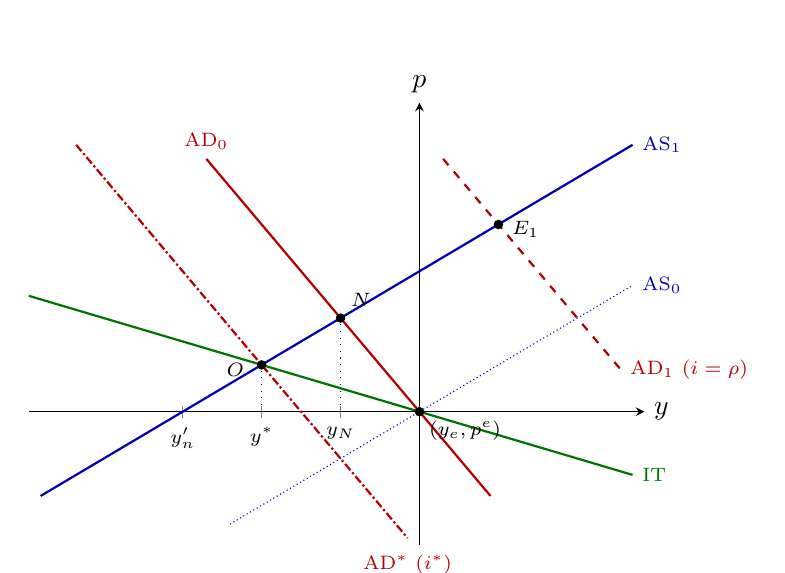
\begin{tikzpicture}
\begin{axis}[width=9.4cm,height=7.2cm,axis lines=middle,xmin=-1.65,xmax=0.95,ymin=-0.95,ymax=2.2,clip=false,
  xlabel={$y$},ylabel={$p$},xtick={-1,-0.6667,-0.3333},xticklabels={$y_n'$,$y^\ast$,$y_N$},ytick=\empty,
  every tick label/.append style={font=\scriptsize},x label style={anchor=west},y label style={anchor=south}]
\addplot[densely dotted,blue!70!black,domain=-0.8:0.9]{x};
\addplot[thick,blue!70!black,domain=-1.6:0.9]{x+1};
\addplot[thick,green!45!black,domain=-1.65:0.9]{-x/2};
\addplot[thick,red!70!black,dashed,domain=0.1:0.85]{2-2*x};
\addplot[thick,red!70!black,domain=-0.9:0.3]{-2*x};
\addplot[thick,red!70!black,densely dashdotted,domain=-1.45:-0.05]{-1-2*x};
\node[font=\scriptsize,blue!70!black,anchor=west] at (axis cs:0.9,0.9){AS$_0$};
\node[font=\scriptsize,blue!70!black,anchor=west] at (axis cs:0.9,1.9){AS$_1$};
\node[font=\scriptsize,green!45!black,anchor=west] at (axis cs:0.9,-0.45){IT};
\node[font=\scriptsize,red!70!black,anchor=west] at (axis cs:0.85,0.3){AD$_1$ ($i=\rho$)};
\node[font=\scriptsize,red!70!black,anchor=south] at (axis cs:-0.9,1.8){AD$_0$};
\node[font=\scriptsize,red!70!black,anchor=north] at (axis cs:-0.05,-0.95){AD$^\ast$ ($i^\ast$)};
\addplot[only marks,mark=*,mark size=1.5pt]coordinates{(0.3333,1.3333)(-0.3333,0.6667)(-0.6667,0.3333)(0,0)};
\node[font=\scriptsize,anchor=west] at (axis cs:0.35,1.3){$E_1$};
\node[font=\scriptsize,anchor=south west] at (axis cs:-0.33,0.68){$N$};
\node[font=\scriptsize,anchor=east] at (axis cs:-0.7,0.3){$O$};
\node[font=\scriptsize,anchor=north west] at (axis cs:0,0){$(y_e,p^e)$};
\draw[dotted](axis cs:-0.6667,0)--(axis cs:-0.6667,0.3333);
\draw[dotted](axis cs:-0.3333,0)--(axis cs:-0.3333,0.6667);
\end{axis}
\end{tikzpicture}\\
{\footnotesize Figure 6. The tax shifts AS from AS$_0$ to AS$_1$ (through $(y_n',p^e)$); the news shifts AD from AD$_0$ to
AD$_1$. With $i=\rho$ the economy is at $E_1$. Offsetting the news alone brings AD back to AD$_0$ and the economy to
$N$. The optimum $O$ is where AS$_1$ meets the IT line; drawn for $\phi=2>\sigma=0.5$, so the bank raises $i$ beyond
the news offset, to AD$^\ast$. ($\kappa=1$, $\Gamma d\bar a=m=1$.)}
\end{minipage}\end{center}
\intuicao{Two shocks, two different jobs. The news is a demand shock with no trade-off: offset it fully. The tax is a
cost shock that drives a wedge between natural and efficient output: no rate fixes both gaps, so the convex loss
spreads the miss, and $\phi$ says how much of it goes into prices.}
\refbib{Benigno (2015) \S11, eqs.~(33)--(35), Fig.~14, pp.~521--523; \S7, Fig.~9, pp.~513--514 (mark-up shocks; taxes in
$1+\mu$); \S4.4, p.~509.}
\rubrica{
\item AS shifts up/left, $y_e$ does not move, AD shift from the news only: 0.15 pt.
\item Why AS is the constraint; substitution into $L$: 0.15 pt.
\item Targeting rule $(y-y_e)+\phi(p-p^e)=0$ from $dL/dy=0$: 0.2 pt.
\item $y^\ast$, $p^\ast$: 0.15 pt. $i^\ast$ with its two components: 0.15 pt.
\item Role of $\phi$: news part independent of $\phi$; mark-up part signed by $\phi-\sigma$; a limit case: 0.1 pt.
\item Graph (AS$_1$, IT, AD before/after, $O$ labelled): 0.1 pt.
\item Differentiating in $i$ with AD as the constraint, or targeting $y_n$ instead of $y_e$: max.\ 0.4 pt. Claiming the whole
response (news included) depends on $\phi$ versus $\sigma$: max.\ 0.6 pt.
}
\gap{Prova 01, 3.c: $dL/dy=0$ along AS not used; the response to news wrongly made to depend on $\phi$.}
\end{sol}

\ifsolucoes\else
\vfill
\begin{center}\footnotesize\textit{End of exam.}\end{center}
\fi

\end{document}
"
% Check fonts: pdffonts <file>.pdf  (all Type 1).
% Every closed form and number in the key: python simulado_codigo/check_simulado_04.py
% Solution format (rules/00_estilo_avaliacao.md §4): each solution opens with a Notation list;
% every equation used later is numbered and cited with \eqref; one operation per displayed line.
% Numbering: Q1 solutions use (G1), (G2)...; Q2 keeps the statement's (1)-(4) and continues from
% (5); Q3 keeps the statement's (AD), (AS), (YN), (LF) and continues the numeric sequence.
% =============================================================================
\documentclass[11pt,a4paper]{article}
\usepackage[utf8]{inputenc}
\usepackage[T1]{fontenc}
\usepackage{lmodern}   % Type 1 vector fonts (replaces PK bitmaps)
\usepackage{cmap}      % ToUnicode CMap -> copyable text and accents
\usepackage[english]{babel}
\usepackage{amsmath,amssymb,amsfonts}
\usepackage[a4paper,margin=2.2cm]{geometry}
\usepackage{enumitem}
\usepackage{fancyhdr}
\usepackage{comment}
% Private cut file per build (sibling sources build in this folder). comment.sty resets
% \CommentCutFile from \DefaultCutFileName at every included environment, so redefine that.
\def\DefaultCutFileName{\def\CommentCutFile{\jobname.cut}}
\usepackage{xcolor}
\usepackage{microtype}
\usepackage{booktabs}
\usepackage{needspace}
\usepackage{pgfplots}
\pgfplotsset{compat=1.18}
\usetikzlibrary{arrows.meta}

% ====================== CONFIGURATION ======================
\newif\ifsolucoes
\ifdefined\withsolutions\solucoestrue\else\solucoesfalse\fi

\newcommand{\disciplina}{Macroeconomics I --- MPE Insper}
\newcommand{\listatema}{Mock Exam 4}

% ====================== MACHINERY ======================
\ifsolucoes\includecomment{sol}\else\excludecomment{sol}\fi

\pagestyle{fancy}\fancyhf{}
\lhead{\footnotesize\disciplina}
\rhead{\footnotesize \listatema\ifsolucoes{} --- Solutions and Rubric\fi}
\cfoot{\footnotesize\thepage}
\renewcommand{\headrulewidth}{0.3pt}
\setlength{\headheight}{14pt}
\setlist{topsep=2pt,itemsep=2pt}

% \questao{number}{points}{statement}
\newcommand{\questao}[3]{\Needspace{12\baselineskip}\bigskip\noindent
  {\large\bfseries\color{blue!55!black}Question #1}\ \textbf{(#2 points)}\par\smallskip\noindent #3\par}
% \item-like heading: \sub{2.a}{1 point}
\newcommand{\sub}[2]{\Needspace{8\baselineskip}\par\medskip\noindent\textbf{#1 (#2)}~}
\newcommand{\resolespaco}[1][6cm]{\ifsolucoes\else\par\textit{Solution:}\vspace{#1}\par\fi}
\newcommand{\passo}[2]{\par\smallskip\noindent\textbf{Step --- #1.}~#2}
\newcommand{\intuicao}[1]{\par\smallskip\noindent\textit{Intuition.}~#1}
\newcommand{\refbib}[1]{\par\smallskip\noindent{\footnotesize\color{black!60}\textbf{Ref:} #1}}
\newcommand{\gap}[1]{\par\smallskip\noindent{\footnotesize\color{red!55!black}\textbf{Gap targeted:} #1}}
\newcommand{\trap}[1]{\par\smallskip\noindent{\small\color{red!55!black}\#~#1}}
\newcommand{\rubrica}[1]{\par\smallskip\noindent\textbf{Grading rubric.}\begin{itemize}[leftmargin=1.4em,topsep=1pt]#1\end{itemize}}
\newenvironment{notacao}{\par\smallskip\noindent\textbf{Notation.}\begin{itemize}[leftmargin=1.4em,topsep=1pt,itemsep=0pt]\small}{\end{itemize}}
\allowdisplaybreaks

% =============================================================================
\begin{document}
\begin{center}
  {\Large\bfseries \disciplina}\\[2pt]
  {\large \listatema\ (Simulado 4) --- 2026, 3rd term}\ifsolucoes\\[2pt]\textit{Solutions and Grading Rubric}\fi
\end{center}
\vspace{2pt}

{\footnotesize\noindent\textbf{Instructions.} Three questions, 10 points in total. Suggested time:
2 hours, closed book, non-programmable calculator allowed. Show every step: a number or a formula
without the argument that produces it earns little. When an item says \emph{explain},
\emph{justify} or \emph{show graphically}, the explanation and the graph are graded on their own
lines: label the axes and every curve, mark the initial and the new point, and indicate the
direction of every shift. Where an item lists several approaches or several choice variables,
answer \emph{each} of them. Box your final answers. Notation: Kurlat (2020) in Questions 1--2,
Benigno (2015) in Question 3.\par}

% =============================================================================
\renewcommand{\theequation}{G\arabic{equation}}% Q1 solution equations: (G1), (G2)...
\questao{1}{1.5}{A simplified economy has, at first, no government. Values are in R\$ million
for one year. A coffee farm in Minas Gerais (Firm F) grows beans worth 400 and sells all of them
to a roastery (Firm R); F uses no inputs and pays 250 in wages. Firm R buys the 400 of beans and
imports packaging worth 100 from abroad; it sells roasted coffee worth 700 to domestic households
and worth 200 to foreign buyers, and pays 300 in wages. Each firm keeps whatever is left as profit.}

\sub{1.a}{0.5 point} Calculate the GDP of this economy by the product, the income and the
expenditure approaches, explaining precisely the concept used in each. Explain why the imported
packaging does not count in GDP, although Firm R used it to produce.
\resolespaco[5.5cm]
\begin{sol}
\begin{notacao}
\item F, R: the coffee farm and the roastery. All values in R\$ million for one year.
\item $VA_j\ge0$: value added of firm $j$, its production minus the intermediate inputs it uses up.
\item $W_j\ge0$: wages paid by firm $j$. $\Pi_j$: its profit (operating surplus), whatever is left
after wages; it can be of either sign.
\item $C$, $I$, $G$: household consumption, investment and government purchases (final domestic
uses). $X\ge0$, $M\ge0$: exports and imports. In 1.a, $I=G=0$.
\end{notacao}
\passo{0, the definitions used below}{GDP is the market value of the \emph{final} goods and
services produced in the territory in the year. It is computed three ways, which must agree:}
\begin{align}
\text{GDP} &= \textstyle\sum_j VA_j, \label{q1:prod}\\
VA_j &= \text{production}_j-\text{intermediate inputs}_j, \label{q1:va}\\
\Pi_j &= VA_j-W_j, \label{q1:profit}\\
\text{GDP} &= \textstyle\sum_j (W_j+\Pi_j), \label{q1:inc}\\
\text{GDP} &= C+I+G+X-M. \label{q1:exp}
\end{align}
\passo{product (value added)}{F uses no inputs; R uses the beans and the imported packaging.
Using \eqref{q1:va} for each firm:}
\begin{align}
VA_F &= 400-0=400, \label{q1a:vaF}\\
VA_R &= (700+200)-400-100\nonumber\\
&= 900-500\nonumber\\
&= 400. \label{q1a:vaR}
\end{align}
Summing \eqref{q1a:vaF} and \eqref{q1a:vaR} with \eqref{q1:prod}:
\begin{equation}
\text{GDP}=400+400=\boxed{800}. \label{q1a:gdp}
\end{equation}
\passo{income (factor payments)}{Profit is what is left of value added after wages. Using
\eqref{q1:profit} with \eqref{q1a:vaF} and \eqref{q1a:vaR}:}
\begin{align}
\Pi_F &= 400-250=150, \label{q1a:piF}\\
\Pi_R &= 400-300=100. \label{q1a:piR}
\end{align}
Add wages and profits, then apply \eqref{q1:inc}:
\begin{align*}
W_F+W_R &= 250+300=550,\\
\Pi_F+\Pi_R &= 150+100=250,\\
\text{GDP} &= 550+250=\boxed{800}.
\end{align*}
\passo{expenditure (final uses)}{The final uses are $C=700$, $I=0$, $G=0$, $X=200$ and
$M=100$. By \eqref{q1:exp}:}
\[
\text{GDP}=700+0+0+200-100=\boxed{800}.
\]
\passo{imports}{The packaging was produced abroad: its 100 is \emph{foreign} value added. In the
product approach it is an intermediate input of R and is subtracted from R's production in
\eqref{q1a:vaR}. In the expenditure approach \eqref{q1:exp}, $C$ and $X$ are measured at purchaser
prices and already contain the packaging, so $-M$ takes it back out. GDP measures what is produced
\emph{in the territory}.}
\trap{Adding sales, $400+900=1300$, counts the beans twice (once as F's sale, once inside R's price) and
counts foreign packaging. The three approaches agree because they are three ways of adding up the same
value added.}
\intuicao{Every real that a final buyer pays for coffee ends up as somebody's income: F's workers and
owners, R's workers and owners, or the foreign packaging producer. Take the foreigner out and the three
columns must match.}
\refbib{Kurlat \S1.1, pp.~15--21 (value added, the three approaches, imports).}
\rubrica{
\item Each approach with the right concept and the number 800: 0.15 pt each (0.45).
\item Why imports are excluded (foreign value added; $-M$ corrects purchaser prices): 0.05 pt.
\item Only one approach, number right: max.\ 0.2 pt. Summing sales (1300) or forgetting $-M$ (900): 0 for that line.
}
\end{sol}

\sub{1.b}{0.5 point} Suppose instead that in the same year households buy only 600 of roasted
coffee. Firm R produces exactly as before and keeps the remaining roasted coffee in its warehouse at
the end of the year, valued at its selling price. Nothing else changes. Calculate, justifying, the
GDP by the product, income and expenditure approaches, compare it with the value in 1.a and explain
what the comparison indicates. Then explain what the sale of that stock to households in the
following year adds to the following year's GDP, other things equal.
\resolespaco[6cm]
\begin{sol}
\begin{notacao}
\item As in 1.a. New: $\Delta\text{inventories}$, the change in R's stock of unsold roasted coffee
during the year, valued at its selling price. It is part of $I$ and can be negative (a drawdown).
\end{notacao}
\passo{what changed}{R's production is unchanged; only its destination moved: households,
exports, and the part left unsold in the warehouse.}
\begin{equation}
\text{production}_R=600+200+100=900. \label{q1b:prodR}
\end{equation}
An unsold good that was produced is a \textbf{change in inventories}, a component of investment:
\begin{equation}
I=\Delta\text{inventories}=100. \label{q1b:inv}
\end{equation}
\passo{product}{F is unchanged, $VA_F=400$ by \eqref{q1a:vaF}. Using \eqref{q1:va} with
\eqref{q1b:prodR}:}
\begin{align*}
VA_R &= 900-400-100\\
&= 400.
\end{align*}
By \eqref{q1:prod}, GDP $=400+400=\boxed{800}$.
\passo{income}{R's operating surplus is measured on production, the stock valued at 100. Using
\eqref{q1:profit}:}
\begin{align*}
\Pi_R &= 900-500-300\\
&= 100.
\end{align*}
Wages are $250+300=550$ and profits $150+100=250$, with $\Pi_F$ from \eqref{q1a:piF}. By
\eqref{q1:inc}, GDP $=550+250=\boxed{800}$.
\passo{expenditure}{Now $C=600$, $I=100$ from \eqref{q1b:inv}, $G=0$, $X=200$, $M=100$. By
\eqref{q1:exp}:}
\[
\text{GDP}=600+100+0+200-100=\boxed{800}.
\]
\passo{comparison}{GDP is the same as \eqref{q1a:gdp}: \textbf{GDP measures production, not sales}.
Only the composition of final demand moved, $C\downarrow100$ and $I\uparrow100$. A firm that cannot
sell is recorded as having invested in its own stock (involuntary, in this case).}
\passo{next year}{Households buy the 100 from stock, so $C$ rises by 100 and inventory investment
is $-100$ (a drawdown). The net contribution to next year's GDP, by \eqref{q1:exp}:}
\begin{align*}
\Delta C &= +100,\\
\Delta I=\Delta\text{inventories} &= -100,\\
\Delta\text{GDP} &= 100-100=\boxed{0}.
\end{align*}
The coffee was counted in the year it was produced; counting it again when sold would double-count it.
\intuicao{Inventories are the entry that makes the expenditure column add up when sales and production
differ. Without it the expenditure side would read $600+200-100=700\neq800$.}
\refbib{Kurlat \S1.1, p.~18 (inventories and their drawdown), pp.~15--21.}
\rubrica{
\item Three approaches with 800 and the inventory entry in $I$: 0.1 pt each (0.3).
\item Comparison: production vs sales, $C$ replaced by $I$: 0.1 pt.
\item Next year: $+C$, $-I$, net zero, with the reason: 0.1 pt.
\item GDP $=700$ (unsold output treated as not produced): max.\ 0.1 pt. One approach only: max.\ 0.25 pt.
}
\end{sol}

\sub{1.c}{0.5 point} Return to the situation of 1.a. The government now collects a lump-sum tax
of 200 from households and uses it to: (i) pay 120 in wages to nurses in public clinics, which treat
patients free of charge; (ii) buy 30 of imported medicines, handed out free at those clinics;
(iii) pay 50 in cash transfers to low-income families (Bolsa Fam\'ilia). Households' purchases of
roasted coffee stay at 700 and nothing else changes. Calculate, justifying, the GDP by the product,
income and expenditure approaches, compare it with 1.a and explain what the comparison indicates.
Explain why GDP does not rise by 200.
\resolespaco[6.5cm]
\begin{sol}
\begin{notacao}
\item As in 1.a. New: the public clinics as a producer, with value added $VA_{\text{clinics}}$.
\item $T=200$: the lump-sum tax. $TR=50$: the cash transfers. Both are flows between households and
government with nothing produced in exchange.
\end{notacao}
\passo{valuing a free service}{Public health care has no market price, so its output is valued
\textbf{at cost}, wages plus inputs:}
\begin{equation}
\text{output}_{\text{clinics}}=120+30=150. \label{q1c:out}
\end{equation}
The medicines are an intermediate input of the clinics. Using \eqref{q1:va} with \eqref{q1c:out}:
\begin{equation}
VA_{\text{clinics}}=150-30=120. \label{q1c:va}
\end{equation}
\passo{product}{Sum \eqref{q1a:vaF}, \eqref{q1a:vaR} and \eqref{q1c:va} with \eqref{q1:prod}:}
\begin{equation}
\text{GDP}=400+400+120=\boxed{920}. \label{q1c:gdp}
\end{equation}
\passo{income}{The clinics have no operating surplus: output is defined as cost, so by
\eqref{q1:profit} their profit is $120-120=0$. Adding up and applying \eqref{q1:inc}:}
\begin{align*}
\text{wages} &= 250+300+120=670,\\
\text{profits} &= 150+100+0=250,\\
\text{GDP} &= 670+250=\boxed{920}.
\end{align*}
\passo{expenditure}{$G=150$ is the clinics' output \eqref{q1c:out}, consumed on behalf of
households. Imports now include the medicines:}
\[
M=100+30=130.
\]
With $C=700$, $I=0$ and $X=200$, by \eqref{q1:exp}:
\[
\text{GDP}=700+0+150+200-130=\boxed{920}.
\]
\passo{what is left out, and why}{\textbf{The tax} (200) is a transfer from households to the
government, not a payment for a good: it is in no column. \textbf{Transfers} (50) buy nothing in
exchange: they are not in $G$ and not factor income (if the families spent them, the spending would
appear in $C$; here $C$ is unchanged by assumption). \textbf{Imported medicines} (30) enter $G$ but are
removed by $-M$: foreign value added.}
\passo{comparison}{Subtract \eqref{q1a:gdp} from \eqref{q1c:gdp}:}
\[
\Delta\text{GDP}=920-800=\boxed{120},
\]
the value added of public health care \eqref{q1c:va}, i.e.\ the nurses' wages. Not by 200 (the tax
is a financing flow), not by 150 (30 of $G$ is imported), not by 50 (transfers are redistribution).
\intuicao{Valuing government output at cost has a consequence: measured public-sector value added equals
its wage bill. If the nurses treated twice as many patients for the same pay, GDP would not record it.}
\refbib{Kurlat \S1.1, p.~20 (Example 1.7, government output at cost; Example 1.8, transfers), pp.~15--21.}
\rubrica{
\item Three approaches with 920, clinics' output at cost and $VA=120$: 0.1 pt each (0.3).
\item Tax, transfers and imported medicines each correctly excluded, with the reason: 0.1 pt.
\item Comparison: $+120$ is the nurses' value added: 0.1 pt.
\item Transfers counted in $G$ (GDP 970) or tax counted (1000): max.\ 0.2 pt. Medicines not netted by $M$ (950): $-0.1$.
}
\gap{Prova 01, 1.b--1.c: the three approaches were asked and only one was given; the classification of a
final use (there: software as investment; here: inventories as investment, clinics' output as $G$).}
\end{sol}

% =============================================================================
\questao{2}{5.5}{Consider an economy described by the Solow model, in which the aggregate variables
satisfy:
\begin{align}
Y_t &= K_t^{\alpha}(A_tL_t)^{1-\alpha}, \tag{1}\label{q2:Y}\\
K_{t+1} &= (1-\delta)K_t+s\,Y_t, \tag{2}\label{q2:K}\\
L_{t+1} &= (1+n)L_t, \tag{3}\label{q2:L}\\
A_{t+1} &= (1+g)A_t, \tag{4}\label{q2:A}
\end{align}
with $\{\alpha,\delta,s\}\in(0,1)$ and $n,g\geq0$.}
\setcounter{equation}{4}\renewcommand{\theequation}{\arabic{equation}}% Q2-Q3 continue from (5)

\sub{2.a}{1 point} Define the stationary variables, per efficiency unit of labour, with a tilde
($\tilde k_t$, $\tilde y_t$), and find an expression for $\tilde k_{t+1}/\tilde k_t$ and then the
steady-state value of $\tilde k$, denoted $\tilde k_{SS}$. Show the steady state graphically. Along
the steady state, at what rates do output per worker $y_t=Y_t/L_t$ and aggregate output $Y_t$ grow?
Justify, and explain why output per worker is not a stationary variable here.
\resolespaco[7cm]
\begin{sol}
\begin{notacao}
\item $Y_t$, $K_t$, $C_t>0$: aggregate output, capital and consumption. $L_t>0$: number of workers.
\item $A_t>0$: labour-augmenting technology; $A_tL_t$ is labour in efficiency units.
\item $\alpha\in(0,1)$: elasticity of output with respect to capital (capital's income share).
$\delta\in(0,1)$: depreciation rate. $s\in(0,1)$: saving rate. $n\ge0$: labour-force growth rate.
$g\ge0$: growth rate of technology.
\item $\tilde k_t$, $\tilde y_t$, $\tilde c_t>0$: capital, output and consumption per efficiency unit
of labour. $k_t=K_t/L_t$, $y_t=Y_t/L_t$: per worker.
\item $\xi\equiv(1+g)(1+n)-(1-\delta)>0$: break-even investment per unit of $\tilde k$ (defined in
step 3). $\tilde k_{SS}$, $\tilde y_{SS}$: steady-state values.
\end{notacao}
\passo{stationary variables}{Technology and labour both grow, so the variables that settle down are
those per efficiency unit:}
\begin{equation}
\tilde k_t\equiv\frac{K_t}{A_tL_t},\qquad \tilde y_t\equiv\frac{Y_t}{A_tL_t},\qquad
\tilde c_t\equiv\frac{C_t}{A_tL_t}. \label{q2a:def}
\end{equation}
Divide \eqref{q2:Y} by $A_tL_t$ and use \eqref{q2a:def}:
\begin{align}
\tilde y_t &= \frac{K_t^{\alpha}(A_tL_t)^{1-\alpha}}{A_tL_t}\nonumber\\
&= K_t^{\alpha}(A_tL_t)^{-\alpha}\nonumber\\
&= \left(\frac{K_t}{A_tL_t}\right)^{\alpha}\nonumber\\
&= \tilde k_t^{\alpha}. \label{q2a:y}
\end{align}
\passo{law of motion}{Multiply \eqref{q2:A} by \eqref{q2:L}:}
\begin{align}
A_{t+1}L_{t+1} &= \big[(1+g)A_t\big]\big[(1+n)L_t\big]\nonumber\\
&= (1+g)(1+n)A_tL_t. \label{q2a:AL}
\end{align}
Divide \eqref{q2:K} by \eqref{q2a:AL}. The second line splits the fraction, the third uses
\eqref{q2a:def}, the fourth \eqref{q2a:y}:
\begin{align}
\tilde k_{t+1} &= \frac{(1-\delta)K_t+sY_t}{(1+g)(1+n)A_tL_t}\nonumber\\
&= \frac{(1-\delta)\frac{K_t}{A_tL_t}+s\frac{Y_t}{A_tL_t}}{(1+g)(1+n)}\nonumber\\
&= \frac{(1-\delta)\tilde k_t+s\tilde y_t}{(1+g)(1+n)}\nonumber\\
&= \frac{(1-\delta)\tilde k_t+s\tilde k_t^{\alpha}}{(1+g)(1+n)}. \label{q2a:lom}
\end{align}
Divide \eqref{q2a:lom} by $\tilde k_t$:
\begin{equation}
\boxed{\frac{\tilde k_{t+1}}{\tilde k_t}=\frac{1-\delta+s\,\tilde k_t^{\alpha-1}}{(1+g)(1+n)}} \label{q2a:ratio}
\end{equation}
\passo{steady state}{Set \eqref{q2a:ratio} equal to 1 and isolate the term in $\tilde k$:}
\begin{align*}
1 &= \frac{1-\delta+s\tilde k^{\alpha-1}}{(1+g)(1+n)}\\
(1+g)(1+n) &= 1-\delta+s\tilde k^{\alpha-1}\\
s\tilde k^{\alpha-1} &= (1+g)(1+n)-(1-\delta).
\end{align*}
Call the right side $\xi$; expanding the product,
\begin{equation}
\xi\equiv(1+g)(1+n)-(1-\delta)=n+g+ng+\delta\ (\approx n+g+\delta). \label{q2a:xi}
\end{equation}
Using \eqref{q2a:xi}:
\begin{align*}
s\tilde k^{\alpha-1} &= \xi\\
\tilde k^{1-\alpha} &= \frac{s}{\xi}.
\end{align*}
Raise both sides to the power $1/(1-\alpha)$:
\begin{equation}
\boxed{\tilde k_{SS}=\left(\frac{s}{(1+g)(1+n)-(1-\delta)}\right)^{\frac{1}{1-\alpha}}} \label{q2a:kss}
\end{equation}
Evaluate \eqref{q2a:y} at \eqref{q2a:kss}, writing its denominator as $\xi$ by \eqref{q2a:xi}:
\begin{align}
\tilde y_{SS} &= \tilde k_{SS}^{\alpha}\nonumber\\
&= \left[\left(\frac{s}{\xi}\right)^{\frac{1}{1-\alpha}}\right]^{\alpha}\nonumber\\
&= \left(\frac{s}{\xi}\right)^{\frac{\alpha}{1-\alpha}}. \label{q2a:yss}
\end{align}
Multiplying the condition $s\tilde k^{\alpha-1}=\xi$ by $\tilde k$ gives the steady state as
investment equal to break-even investment:
\begin{equation}
s\tilde k_{SS}^{\alpha}=\xi\,\tilde k_{SS}. \label{q2a:break}
\end{equation}
\passo{stability}{In \eqref{q2a:ratio}, $\alpha-1<0$, so $\tilde k_{t+1}/\tilde k_t$ falls as
$\tilde k_t$ rises: it is $>1$ below $\tilde k_{SS}$ and $<1$ above. The positive steady state is
unique and every $\tilde k_0>0$ converges to it. Graphically (Figure 1): investment per efficiency
unit $s\tilde k^{\alpha}$ against break-even investment $\xi\tilde k$, the two sides of
\eqref{q2a:break}; $\xi$ is the amount needed to equip the new workers ($n$), the new efficiency
units ($g$) and to replace depreciation ($\delta$).}
\passo{growth rates}{In the steady state $\tilde y=\tilde y_{SS}$ is constant. Invert
\eqref{q2a:def}:}
\begin{align}
y_t &= \frac{Y_t}{L_t}=A_t\,\tilde y_{SS}, \label{q2a:ypw}\\
Y_t &= A_tL_t\,\tilde y_{SS}. \label{q2a:Yagg}
\end{align}
Take ratios of consecutive periods, using \eqref{q2:A} in \eqref{q2a:ypw} and \eqref{q2a:AL} in
\eqref{q2a:Yagg}:
\begin{align*}
\frac{y_{t+1}}{y_t} &= \frac{A_{t+1}\,\tilde y_{SS}}{A_t\,\tilde y_{SS}}\\
&= \frac{\big[(1+g)A_t\big]\tilde y_{SS}}{A_t\,\tilde y_{SS}}\\
&= 1+g &&\Rightarrow\ y_t\text{ grows at }\boxed{g},\\
\frac{Y_{t+1}}{Y_t} &= \frac{A_{t+1}L_{t+1}\,\tilde y_{SS}}{A_tL_t\,\tilde y_{SS}}\\
&= \frac{\big[(1+g)(1+n)A_tL_t\big]\tilde y_{SS}}{A_tL_t\,\tilde y_{SS}}\\
&= (1+g)(1+n) &&\Rightarrow\ Y_t\text{ grows at }\boxed{(1+g)(1+n)-1=g+n+gn}.
\end{align*}
The same holds for $k_t=K_t/L_t$ ($g$) and $K_t$ ($g+n+gn$); $K/Y$ is constant.
\passo{why $y$ is not stationary}{Each period every worker supplies $1+g$ times more efficiency units.
Capital per worker must grow at $g$ just to keep pace, so per-worker variables have a trend; dividing by
$A_tL_t$ removes it. Long-run growth of $y$ comes only from $g$, which the model takes as given.}
\begin{center}
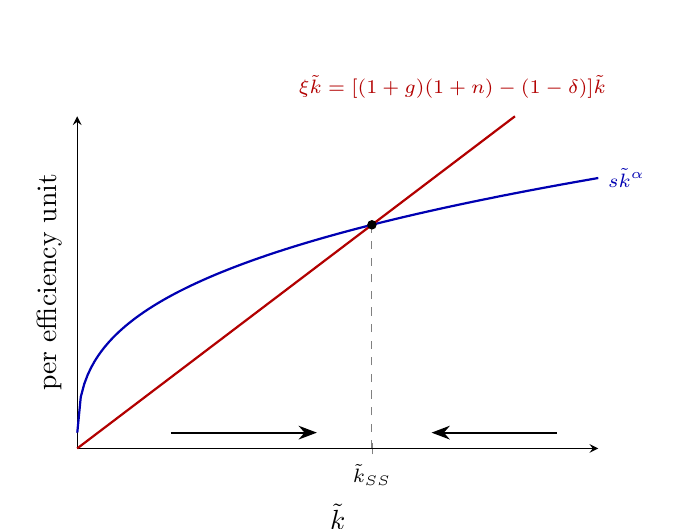
\begin{tikzpicture}
\begin{axis}[width=8.2cm,height=5.8cm,axis lines=left,xmin=0,xmax=5,ymin=0,ymax=0.42,clip=false,
  xlabel={$\tilde k$},ylabel={per efficiency unit},xtick={2.828},xticklabels={$\tilde k_{SS}$},ytick=\empty,
  every tick label/.append style={font=\scriptsize}]
\addplot[domain=0.001:5,samples=150,thick,blue!70!black]{0.2*x^(1/3)};
\addplot[domain=0:4.2,thick,red!70!black]{0.1*x};
\node[font=\scriptsize,blue!70!black,anchor=west] at (axis cs:5,0.342){$s\tilde k^{\alpha}$};
\node[font=\scriptsize,red!70!black,anchor=south] at (axis cs:3.6,0.43){$\xi\tilde k=[(1+g)(1+n)-(1-\delta)]\tilde k$};
\draw[dashed,gray](axis cs:2.828,0)--(axis cs:2.828,0.2828);
\addplot[only marks,mark=*,mark size=1.5pt]coordinates{(2.828,0.2828)};
\draw[-{Stealth},thick](axis cs:0.9,0.02)--(axis cs:2.3,0.02);
\draw[-{Stealth},thick](axis cs:4.6,0.02)--(axis cs:3.4,0.02);
\end{axis}
\end{tikzpicture}\\
{\footnotesize Figure 1. Steady state per efficiency unit. Left of $\tilde k_{SS}$ investment exceeds break-even
investment and $\tilde k$ rises; right of it, $\tilde k$ falls. (Drawn for $\alpha=1/3$, $s=0.2$, $\xi=0.1$.)}
\end{center}
\intuicao{Solow with technological progress is the no-progress model with one change of units: count
workers in efficiency units and the economy settles at a constant $\tilde k$; in per-worker units that same
point is a path growing at $g$.}
\refbib{Kurlat \S4.2, pp.~57--61 (law of motion, steady state, stability); \S4.5, pp.~69--72 (efficiency units,
balanced growth path).}
\rubrica{
\item Stationary variables defined and $\tilde y=\tilde k^{\alpha}$: 0.2 pt.
\item Ratio $\tilde k_{t+1}/\tilde k_t$ with $(1+g)(1+n)$ in the denominator: 0.3 pt.
\item $\tilde k_{SS}$: 0.2 pt. Diagram (axes, both curves named, $\tilde k_{SS}$ marked): 0.1 pt.
\item Growth rates of $y$ and $Y$ with the reason: 0.2 pt.
\item Dividing (2) by $A_tL_t$ instead of $A_{t+1}L_{t+1}$ (no $(1+g)(1+n)$): max.\ 0.5 pt. Working with $K/L$ as if stationary: max.\ 0.4 pt.
}
\end{sol}

\sub{2.b}{1 point} Show which saving rate maximises steady-state consumption per efficiency unit
of labour (the golden-rule rate, $s_{GR}$). Explain why the same $s_{GR}$ also maximises consumption
per worker at every date along the steady state, and how a faster rate of technological progress
$g$ changes $s_{GR}$ and $\tilde k_{GR}$. Give the economic intuition.
\resolespaco[7cm]
\begin{sol}
\begin{notacao}
\item As in 2.a. New: $\tilde c_{SS}(s)$, steady-state consumption per efficiency unit as a function
of the saving rate.
\item $f(\tilde k)\equiv\tilde k^{\alpha}$: output per efficiency unit, by \eqref{q2a:y}.
\item $s_{GR}\in(0,1)$, $\tilde k_{GR}>0$: golden-rule saving rate and capital per efficiency unit.
\item $c_t\equiv C_t/L_t$: consumption per worker. $A_0>0$: technology at date 0.
\end{notacao}
\passo{consumption in steady state}{Consumption is the part of output not saved:}
\begin{equation}
\tilde c_t=(1-s)\,\tilde y_t. \label{q2b:c}
\end{equation}
Substitute \eqref{q2a:yss} into \eqref{q2b:c}, carrying the exponent $\alpha$ of
$\tilde k_{SS}^{\alpha}$ through the substitution:
\begin{align}
\tilde c_{SS}(s) &= (1-s)\,\tilde k_{SS}^{\alpha}\nonumber\\
&= (1-s)\left[\left(\frac{s}{\xi}\right)^{\frac{1}{1-\alpha}}\right]^{\alpha}\nonumber\\
&= (1-s)\left(\frac{s}{\xi}\right)^{\frac{\alpha}{1-\alpha}}. \label{q2b:css}
\end{align}
\passo{first-order condition}{Take the log of \eqref{q2b:css}:}
\begin{equation}
\ln\tilde c_{SS}=\ln(1-s)+\frac{\alpha}{1-\alpha}\ln s-\frac{\alpha}{1-\alpha}\ln\xi. \label{q2b:log}
\end{equation}
Differentiate \eqref{q2b:log} with respect to $s$ and set it to zero:
\begin{equation}
\frac{d\ln\tilde c_{SS}}{ds}=-\frac{1}{1-s}+\frac{\alpha}{(1-\alpha)s}=0. \label{q2b:foc}
\end{equation}
Multiply \eqref{q2b:foc} by $(1-\alpha)s(1-s)>0$:
\begin{align*}
-(1-\alpha)s+\alpha(1-s) &= 0\\
\alpha(1-s) &= (1-\alpha)s\\
\alpha-\alpha s &= s-\alpha s\\
\alpha &= s.
\end{align*}
Hence
\begin{equation}
\boxed{s_{GR}=\alpha} \label{q2b:sgr}
\end{equation}
SOC: differentiate \eqref{q2b:foc} once more:
\[
\frac{d^2\ln\tilde c_{SS}}{ds^2}=-\frac{1}{(1-s)^2}-\frac{\alpha}{(1-\alpha)s^2}<0,
\]
so \eqref{q2b:sgr} is a maximum.
\passo{cross-check by $\tilde k$}{Substitute \eqref{q2a:y} into \eqref{q2b:c}, then use the
steady-state condition \eqref{q2a:break}, $s\tilde k^{\alpha}=\xi\tilde k$:}
\begin{align}
\tilde c &= (1-s)\big(\tilde k^{\alpha}\big)\nonumber\\
&= \tilde k^{\alpha}-s\tilde k^{\alpha}\nonumber\\
&= \tilde k^{\alpha}-\big(\xi\tilde k\big). \label{q2b:ck}
\end{align}
Maximise \eqref{q2b:ck} over $\tilde k$:
\begin{equation}
\boxed{f'(\tilde k_{GR})=\alpha\tilde k_{GR}^{\alpha-1}=\xi=(1+g)(1+n)-(1-\delta)} \label{q2b:mpk}
\end{equation}
The marginal product of capital equals break-even investment per unit of capital. Solve
\eqref{q2b:mpk} for $\tilde k_{GR}$:
\begin{equation}
\tilde k_{GR}^{1-\alpha}=\frac{\alpha}{\xi}. \label{q2b:kgr}
\end{equation}
Solve \eqref{q2a:break} for $s$ at $\tilde k_{GR}$ and use \eqref{q2b:kgr} in the third line:
\begin{align*}
s &= \frac{\xi\tilde k_{GR}}{\tilde k_{GR}^{\alpha}}\\
&= \xi\,\tilde k_{GR}^{1-\alpha}\\
&= \xi\cdot\frac{\alpha}{\xi}\\
&= \alpha\ \checkmark
\end{align*}
\passo{per worker, every date}{Invert \eqref{q2a:def} and use \eqref{q2:A}:}
\begin{align}
c_t &= \frac{C_t}{L_t}=A_t\,\tilde c_{SS}\nonumber\\
&= A_0(1+g)^t\,\tilde c_{SS}. \label{q2b:cpw}
\end{align}
Take logs of \eqref{q2b:cpw}:
\begin{equation}
\ln c_t=\ln A_0+t\ln(1+g)+\ln\tilde c_{SS}(s). \label{q2b:lncpw}
\end{equation}
$A_t$ does not depend on $s$, so the $s$ that maximises $\tilde c_{SS}$ raises the whole path
\eqref{q2b:lncpw} by the same amount at every $t$: the golden rule maximises consumption per worker
at \emph{every} date of the steady state.
\passo{effect of $g$}{$g$ does not appear in \eqref{q2b:sgr}: $s_{GR}=\alpha$ is
\textbf{unchanged}. Solving \eqref{q2b:kgr},}
\[
\tilde k_{GR}=\left(\frac{\alpha}{\xi}\right)^{\frac{1}{1-\alpha}},
\]
and by \eqref{q2a:xi}, $\partial\xi/\partial g=1+n>0$, so $\boxed{\tilde k_{GR}\downarrow}$. Faster
progress makes keeping $\tilde k$ constant more expensive (steeper break-even line), so the
consumption-maximising capital per efficiency unit is lower; but the \emph{share} of output to save
does not move, because with Cobb--Douglas the capital income $\alpha\tilde y$ always equals the
break-even investment $\xi\tilde k$ exactly at the golden rule.
\passo{knife-edge check}{$\alpha\to0$: capital is useless and $s_{GR}\to0$ in \eqref{q2b:sgr}.
Dropping the exponent (using $(s/\xi)^{1/(1-\alpha)}$ for $\tilde y$ in \eqref{q2b:css}) gives
$s=1/(2-\alpha)\to1/2$, which fails this test.}
\begin{center}
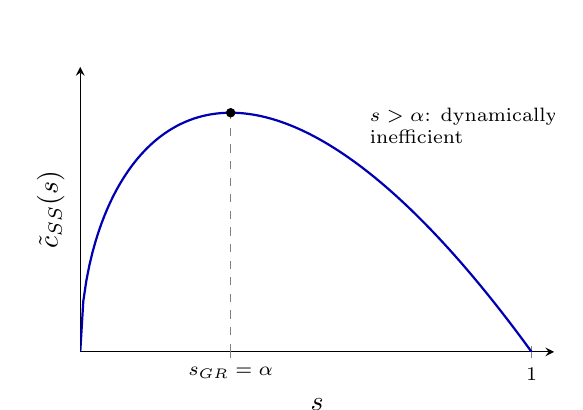
\begin{tikzpicture}
\begin{axis}[width=7.6cm,height=5.2cm,axis lines=left,xmin=0,xmax=1.05,ymin=0,ymax=1.45,
  xlabel={$s$},ylabel={$\tilde c_{SS}(s)$},xtick={0.3333,1},xticklabels={$s_{GR}=\alpha$,$1$},ytick=\empty,
  every tick label/.append style={font=\scriptsize}]
\addplot[domain=0:1,samples=150,thick,blue!70!black]{(1-x)*sqrt(x/0.1)};
\draw[dashed,gray](axis cs:0.3333,0)--(axis cs:0.3333,1.217);
\addplot[only marks,mark=*,mark size=1.5pt]coordinates{(0.3333,1.217)};
\node[font=\scriptsize,anchor=west,align=left] at (axis cs:0.62,1.15){$s>\alpha$: dynamically\\inefficient};
\end{axis}
\end{tikzpicture}\\
{\footnotesize Figure 2. Steady-state consumption per efficiency unit against $s$ (drawn for $\alpha=1/3$, $\xi=0.1$):
zero at $s=0$ (nothing to consume from) and at $s=1$ (nothing consumed), maximum at $s=\alpha$.}
\end{center}
\intuicao{Saving more raises $\tilde k$ and output, but each extra unit of capital also needs $\xi$ of
investment every period just to be kept per efficiency unit. Consumption is maximised when the last unit
of capital produces exactly what it costs to maintain: $f'(\tilde k)=\xi$. Above that point ($s>\alpha$) the
economy could consume more today and forever by saving less.}
\refbib{Kurlat \S4.3, pp.~61--63 (golden rule, $s_{gold}=\alpha$); \S4.5, pp.~69--72.}
\rubrica{
\item $\tilde c_{SS}(s)$ with exponent $\alpha/(1-\alpha)$: 0.3 pt.
\item FOC and $s_{GR}=\alpha$ (SOC or cross-check $f'=\xi$): 0.3 pt.
\item Per-worker consumption at every date maximised: 0.2 pt. Effect of $g$ on $s_{GR}$ and $\tilde k_{GR}$: 0.1 pt.
\item Intuition (marginal product equals break-even cost): 0.1 pt.
\item Exponent dropped in the substitution ($s=1/(2-\alpha)$): max.\ 0.4 pt. Maximising $\tilde k$ (answer $s=1$): max.\ 0.2 pt.
}
\gap{Prova 01, 2.b: the $\sigma$ (here $\alpha$) in the exponent of $c_{SS}$ was dropped.}
\end{sol}

\sub{2.c}{1 point} Consider now the competitive equilibrium of an economy that lasts only two
periods, $t=1,2$. There is an initial capital stock $K_1>0$, which belongs to the representative
firm and depreciates fully once used in period~1. The representative firm maximises profits in
perfectly competitive markets and has production function (1) in both periods, with
$A_2=(1+g)A_1$. The representative consumer owns the firm and receives its profits $\Pi_1$ and
$\Pi_2$. In each period the consumer has one unit of time, which it splits between work $L_t$ and
leisure $1-L_t$, and earns real labour income $w_tA_tL_t$ ($w_t$ is the real wage per efficiency
unit of labour). Income not consumed in period~1 is saved as an asset $a_1$ that pays the real
interest rate $r$; the only asset in this economy is the capital the firm uses in period~2, $K_2$,
which also depreciates fully once used. Intertemporal utility is
\[
U=\ln c_1+\gamma\ln(1-L_1)+\beta\left[\ln c_2+\gamma\ln(1-L_2)\right],\qquad \beta\in(0,1),\ \gamma>0.
\]
Derive and explain the intertemporal budget constraint of this consumer.
\resolespaco[6cm]
\begin{sol}
\begin{notacao}
\item $c_1$, $c_2>0$: consumption in periods 1 and 2. $L_t\in[0,1]$: hours worked; $1-L_t$: leisure
(time endowment normalised to 1).
\item $A_t>0$: technology, with $A_2=(1+g)A_1$. $w_t>0$: real wage per efficiency unit of labour, so
labour income is $w_tA_tL_t$.
\item $\Pi_1$, $\Pi_2$: the firm's profits, paid to the consumer who owns it.
\item $a_1$: asset carried from period 1 to period 2; of either sign for one consumer (in
equilibrium it is the capital $K_2>0$). $r>-1$: real interest rate between the periods.
\item $\beta\in(0,1)$: discount factor. $\gamma>0$: weight of leisure in utility.
\item $H>0$: full lifetime income, the present value of the time endowment plus profits (step 3).
\end{notacao}
\passo{period constraints}{In period 1, uses equal sources:}
\begin{equation}
\boxed{c_1+a_1=w_1A_1L_1+\Pi_1} \label{q2c:b1}
\end{equation}
Period 2 is the last: nothing is left for later, and nobody would lend to a consumer who cannot
repay after period 2. So the consumer spends the asset with its return plus period-2 income:
\begin{equation}
\boxed{c_2=(1+r)a_1+w_2A_2L_2+\Pi_2} \label{q2c:b2}
\end{equation}
Profits appear because the consumer owns the firm; with no initial financial wealth, they are its
only non-labour income besides the return on $a_1$.
\passo{eliminate $a_1$}{Solve \eqref{q2c:b2} for $a_1$:}
\begin{equation}
a_1=\frac{c_2-w_2A_2L_2-\Pi_2}{1+r}. \label{q2c:a1}
\end{equation}
Substitute \eqref{q2c:a1} into \eqref{q2c:b1}:
\[
c_1+\frac{c_2-w_2A_2L_2-\Pi_2}{1+r}=w_1A_1L_1+\Pi_1 .
\]
Move the period-2 income terms to the right side:
\begin{equation}
\boxed{c_1+\frac{c_2}{1+r}=w_1A_1L_1+\Pi_1+\frac{w_2A_2L_2+\Pi_2}{1+r}} \label{q2c:ibc}
\end{equation}
\passo{full-income form}{Value leisure at its opportunity cost, the wage. Add
$w_1A_1(1-L_1)+\frac{w_2A_2(1-L_2)}{1+r}$ to both sides of \eqref{q2c:ibc}; on the right,
$w_tA_tL_t+w_tA_t(1-L_t)=w_tA_t$:}
\begin{align}
&c_1+w_1A_1(1-L_1)+\frac{c_2+w_2A_2(1-L_2)}{1+r}\nonumber\\
&\qquad=\big[w_1A_1L_1+w_1A_1(1-L_1)\big]+\Pi_1+\frac{\big[w_2A_2L_2+w_2A_2(1-L_2)\big]+\Pi_2}{1+r}\nonumber\\
&\qquad=H, \label{q2c:full}
\end{align}
where
\begin{equation}
H\equiv w_1A_1+\Pi_1+\frac{w_2A_2+\Pi_2}{1+r}. \label{q2c:H}
\end{equation}
\passo{reading}{By \eqref{q2c:full}--\eqref{q2c:H}, the \textbf{present value} of lifetime
consumption (and of leisure, priced at the wage) equals the present value of lifetime income: the
value of the whole time endowment plus profits, with period-2 amounts discounted at $1+r$. $a_1$ may
be of either sign for one consumer; it disappears from the lifetime constraint \eqref{q2c:ibc}
because borrowing and lending only move resources across periods at the price $1/(1+r)$. The
constraint binds: $u'>0$, so unspent resources at the end are never optimal.}
\refbib{Kurlat \S6.2, pp.~105--112 (intertemporal budget constraint); \S7.2, pp.~131--137 (time endowment,
labour income); ch.~9, \S9.1 (households own the firms).}
\rubrica{
\item Two period constraints, with $\Pi_1,\Pi_2$ and the labour income of both periods: 0.4 pt.
\item Elimination of $a_1$ to the present-value constraint: 0.3 pt.
\item Explanation as a present-value statement (why $1+r$ discounts, why it binds): 0.3 pt.
\item Profits omitted: $-0.2$. ``Consumption adjusted by $r$'' without the present-value reading: max.\ 0.1 on the last line.
}
\gap{Prova 01, 2.c: firm profits omitted from the budget constraint; reading not stated in present value.}
\end{sol}

\sub{2.d}{1 point} Set up the problem of the consumer of item 2.c and derive the first-order
conditions for \emph{all} of its choice variables, including the equation describing the
intertemporal consumption decision and the consumption--leisure decision in each period. Then find
the equation that gives the optimal $c_1$ as a function only of parameters, prices and levels of
income and wealth, and interpret it economically.
\resolespaco[7cm]
\begin{sol}
\begin{notacao}
\item As in 2.c. New: $\lambda_1$, $\lambda_2>0$, the multipliers on \eqref{q2c:b1} and
\eqref{q2c:b2}: the marginal utility of one more unit of income in period $t$.
\end{notacao}
\passo{problem}{Choice variables: $c_1,c_2,L_1,L_2,a_1$; prices $w_1,w_2,r$ and profits
$\Pi_1,\Pi_2$ are taken as given. Maximise $U$ subject to \eqref{q2c:b1} and \eqref{q2c:b2}, with
one multiplier per period constraint:}
\begin{align}
\mathcal L={}&\ln c_1+\gamma\ln(1-L_1)+\beta\ln c_2+\beta\gamma\ln(1-L_2)\nonumber\\
&+\lambda_1\left[w_1A_1L_1+\Pi_1-c_1-a_1\right]+\lambda_2\left[(1+r)a_1+w_2A_2L_2+\Pi_2-c_2\right]. \label{q2d:lag}
\end{align}
\passo{FOCs}{Differentiate \eqref{q2d:lag} with respect to each choice variable and set the
derivative to zero:}
\begin{align}
c_1:&\quad \frac{1}{c_1}=\lambda_1, \label{q2d:c1}\\
c_2:&\quad \frac{\beta}{c_2}=\lambda_2, \label{q2d:c2}\\
L_1:&\quad \frac{\gamma}{1-L_1}=\lambda_1w_1A_1, \label{q2d:L1}\\
L_2:&\quad \frac{\beta\gamma}{1-L_2}=\lambda_2w_2A_2, \label{q2d:L2}\\
a_1:&\quad \lambda_1=(1+r)\lambda_2. \label{q2d:a1}
\end{align}
Log utility makes every solution interior: as $L_t\to1$ the marginal utility of leisure goes to
infinity, and as $c_t\to0$ that of consumption does.
\passo{Euler (intertemporal)}{Substitute \eqref{q2d:c1} and \eqref{q2d:c2} into \eqref{q2d:a1}:}
\begin{align*}
\left(\frac{1}{c_1}\right) &= (1+r)\left(\frac{\beta}{c_2}\right)\\
\frac{1}{c_1} &= \beta(1+r)\frac{1}{c_2}.
\end{align*}
Multiply by $c_1c_2$:
\begin{equation}
\boxed{c_2=\beta(1+r)\,c_1} \label{q2d:euler}
\end{equation}
The marginal rate of substitution between $c_1$ and $c_2$ equals the relative price $1+r$.
\passo{consumption--leisure (intratemporal)}{Divide \eqref{q2d:L1} by \eqref{q2d:c1}, and
\eqref{q2d:L2} by \eqref{q2d:c2}; the multipliers cancel:}
\begin{align*}
\frac{\gamma/(1-L_1)}{1/c_1} &= \frac{\lambda_1w_1A_1}{\lambda_1},\\
\frac{\beta\gamma/(1-L_2)}{\beta/c_2} &= \frac{\lambda_2w_2A_2}{\lambda_2}.
\end{align*}
\begin{equation}
\boxed{\frac{\gamma c_1}{1-L_1}=w_1A_1} \label{q2d:intra1}
\end{equation}
\begin{equation}
\boxed{\frac{\gamma c_2}{1-L_2}=w_2A_2} \label{q2d:intra2}
\end{equation}
In each period the MRS between leisure and consumption equals the real wage (the price of an hour
of leisure).
\passo{solve for $c_1$}{Express each term on the left of the full-income constraint
\eqref{q2c:full} in terms of $c_1$. From \eqref{q2d:euler}, \eqref{q2d:intra1}, and
\eqref{q2d:intra2} followed by \eqref{q2d:euler}:}
\begin{align}
\frac{c_2}{1+r} &= \frac{\big[\beta(1+r)c_1\big]}{1+r}\nonumber\\
&= \beta c_1, \label{q2d:t1}\\
w_1A_1(1-L_1) &= \gamma c_1, \label{q2d:t2}\\
\frac{w_2A_2(1-L_2)}{1+r} &= \frac{\gamma c_2}{1+r}\nonumber\\
&= \frac{\gamma\big[\beta(1+r)c_1\big]}{1+r}\nonumber\\
&= \beta\gamma c_1. \label{q2d:t3}
\end{align}
Split the fraction in \eqref{q2c:full} and substitute \eqref{q2d:t1}--\eqref{q2d:t3}:
\begin{align*}
c_1+w_1A_1(1-L_1)+\frac{c_2}{1+r}+\frac{w_2A_2(1-L_2)}{1+r} &= H\\
c_1+(\gamma c_1)+(\beta c_1)+(\beta\gamma c_1) &= H\\
c_1(1+\gamma+\beta+\beta\gamma) &= H\\
c_1(1+\beta)(1+\gamma) &= H.
\end{align*}
Divide by $(1+\beta)(1+\gamma)$ and write $H$ out with \eqref{q2c:H}:
\begin{align}
c_1 &= \frac{H}{(1+\beta)(1+\gamma)}\nonumber\\
&= \boxed{\frac{1}{(1+\beta)(1+\gamma)}\left[w_1A_1+\Pi_1+\frac{w_2A_2+\Pi_2}{1+r}\right]} \label{q2d:c1sol}
\end{align}
Then \eqref{q2d:euler}, \eqref{q2d:intra1}--\eqref{q2d:intra2} and \eqref{q2c:b1} give the other
choices:
\begin{align*}
c_2 &= \beta(1+r)\,c_1,\\
1-L_t &= \frac{\gamma c_t}{w_tA_t},\quad t=1,2,\\
a_1 &= w_1A_1L_1+\Pi_1-c_1.
\end{align*}
\passo{interpretation}{By \eqref{q2d:t1}--\eqref{q2d:c1sol}, with log utility the consumer spends fixed shares of full lifetime wealth $H$:
$\frac{1}{(1+\beta)(1+\gamma)}$ on $c_1$, $\frac{\gamma}{(1+\beta)(1+\gamma)}$ on leisure in period 1,
$\frac{\beta}{(1+\beta)(1+\gamma)}$ and $\frac{\beta\gamma}{(1+\beta)(1+\gamma)}$ on period~2.
$c_1$ depends on \emph{lifetime} resources, not on period-1 income alone (permanent income).
$\beta\uparrow\Rightarrow c_1\downarrow$ (patience moves spending to period 2); $\gamma\uparrow\Rightarrow
c_1\downarrow$ for given $H$ (more of full wealth is taken as leisure). Given $H$, $r$ does not enter: for
the shares, the income and substitution effects of $r$ cancel with log utility; $r$ moves $c_1$ only
through the present value of period-2 income in $H$ (a higher $r$ lowers it, so $c_1$ falls).}
\intuicao{Contrast with Prova 01: there work had no utility cost, so $L_1=1$ was a corner and saying so
was the FOC. Here leisure is valued, so hours are an interior choice and the wage is the price of leisure.}
\refbib{Kurlat \S6.2, pp.~105--115 (Euler equation, log closed forms); \S7.2, pp.~131--137 (consumption--leisure);
ch.~9, \S9.1, eq.~(9.1.7)--(9.1.8).}
\rubrica{
\item Problem stated with all five choice variables: 0.1 pt.
\item FOCs for $c_1,c_2$ and the Euler equation: 0.3 pt. FOCs for $L_1$ and $L_2$ (intratemporal conditions): 0.2 pt (0.1 each).
\item FOC for $a_1$ (or the substitution that eliminates it): 0.1 pt.
\item $c_1$ in closed form: 0.2 pt. Interpretation ($H$, $\beta$, $\gamma$, role of $r$): 0.1 pt.
\item No FOC for hours: max.\ 0.6 pt. Substitution route instead of Lagrangian: full credit.
}
\gap{Prova 01, 2.d: FOC for $L_1$ missing (``todas as variáveis de sua escolha'').}
\end{sol}

\sub{2.e}{1 point} Calculate the saving rate of this representative consumer (the share of saving
in the consumer's period-1 income), recalling that markets are perfectly competitive. Find the hours
worked in each period. Then find an expression for $\hat k_2\equiv K_2/A_2$ as a function only of
$\hat k_1\equiv K_1/A_1$ and of parameters. Treating this expression as a law of motion that applies
period after period, draw it with $\hat k_1$ on the horizontal axis and $\hat k_2$ on the vertical
axis, and show graphically the steady state of this economy. Is it stable? Justify.
\resolespaco[8cm]
\begin{sol}
\begin{notacao}
\item As in 2.c--2.d. New: $Y_1$, $Y_2>0$, output in each period by \eqref{q2:Y}; $K_2>0$, the
capital built from period-1 saving.
\item $s^\ast\in(0,1)$: the consumer's saving rate. $\hat k_t\equiv K_t/A_t>0$: capital per unit of
technology.
\item $\phi(\hat k)$: the law of motion $\hat k_{t+1}=\phi(\hat k_t)$. $\hat k_{SS}$: its fixed point.
$\hat k_{GR}$ (Figure 3): the fixed point of the same map with $s=s_{GR}$.
\end{notacao}
\passo{firm, period 1}{The firm owns $K_1$ and hires labour:}
\begin{equation}
\max_{L_1}\ K_1^{\alpha}(A_1L_1)^{1-\alpha}-w_1A_1L_1. \label{q2e:firm1}
\end{equation}
The FOC of \eqref{q2e:firm1}, with $Y_1$ from \eqref{q2:Y}:
\begin{equation}
(1-\alpha)\frac{Y_1}{L_1}=w_1A_1. \label{q2e:foc1}
\end{equation}
Multiply \eqref{q2e:foc1} by $L_1$ to get the wage bill:
\begin{equation}
w_1A_1L_1=(1-\alpha)Y_1. \label{q2e:wb1}
\end{equation}
Profit is output minus the wage bill \eqref{q2e:wb1}:
\begin{align}
\Pi_1 &= Y_1-w_1A_1L_1\nonumber\\
&= Y_1-(1-\alpha)Y_1\nonumber\\
&= \boxed{\alpha Y_1}, \label{q2e:pi1}
\end{align}
the return on the capital the firm owns, paid to its owner.
\passo{firm, period 2}{The firm borrows $K_2$ from the consumer and repays $(1+r)K_2$ (the capital
is used up):}
\begin{equation}
\max_{K_2,L_2}\ K_2^{\alpha}(A_2L_2)^{1-\alpha}-w_2A_2L_2-(1+r)K_2. \label{q2e:firm2}
\end{equation}
The FOCs of \eqref{q2e:firm2}:
\begin{align}
\alpha\frac{Y_2}{K_2} &= 1+r, \label{q2e:r}\\
(1-\alpha)\frac{Y_2}{L_2} &= w_2A_2. \label{q2e:w2}
\end{align}
Multiply \eqref{q2e:r} by $K_2$ and \eqref{q2e:w2} by $L_2$ and subtract both payments from output.
With constant returns:
\begin{align}
\Pi_2 &= Y_2-w_2A_2L_2-(1+r)K_2\nonumber\\
&= Y_2-(1-\alpha)Y_2-\alpha Y_2\nonumber\\
&= \boxed{0}. \label{q2e:pi2}
\end{align}
\passo{market clearing}{The only asset is the capital of period 2, so the asset market clears when}
\begin{equation}
\boxed{a_1=K_2} \label{q2e:mc}
\end{equation}
The goods markets clear when
\begin{align}
c_1+K_2 &= Y_1, \label{q2e:g1}\\
c_2 &= Y_2. \label{q2e:g2}
\end{align}
Labour: $L_t$ supplied $=$ $L_t$ demanded. Check: by \eqref{q2e:r}, \eqref{q2e:w2} and
\eqref{q2e:pi2}, period-2 income in \eqref{q2c:b2} is
\[
(1+r)K_2+w_2A_2L_2+\Pi_2=\alpha Y_2+(1-\alpha)Y_2+0=Y_2 .
\]
\passo{saving rate}{Substitute \eqref{q2e:g2} and \eqref{q2e:r} into the Euler equation
\eqref{q2d:euler}, then multiply by $K_2/Y_2$:}
\begin{align}
(Y_2) &= \beta\left(\frac{\alpha Y_2}{K_2}\right)c_1\nonumber\\
K_2 &= \alpha\beta\,c_1. \label{q2e:K2c1}
\end{align}
Substitute \eqref{q2e:K2c1} into the period-1 goods market \eqref{q2e:g1}:
\begin{align}
c_1+(\alpha\beta c_1) &= Y_1\nonumber\\
c_1 &= \frac{Y_1}{1+\alpha\beta}. \label{q2e:c1}
\end{align}
Substitute \eqref{q2e:c1} into \eqref{q2e:K2c1} and use \eqref{q2e:mc}:
\begin{align}
K_2 &= \alpha\beta\left(\frac{Y_1}{1+\alpha\beta}\right)\nonumber\\
a_1=K_2 &= \frac{\alpha\beta}{1+\alpha\beta}\,Y_1. \label{q2e:a1}
\end{align}
Period-1 income, by \eqref{q2e:wb1} and \eqref{q2e:pi1}:
\begin{align}
w_1A_1L_1+\Pi_1 &= (1-\alpha)Y_1+\alpha Y_1\nonumber\\
&= Y_1. \label{q2e:inc1}
\end{align}
Divide \eqref{q2e:a1} by \eqref{q2e:inc1}:
\begin{align}
s^\ast &= \frac{a_1}{w_1A_1L_1+\Pi_1}\nonumber\\
&= \frac{\left(\frac{\alpha\beta}{1+\alpha\beta}\,Y_1\right)}{(Y_1)}\nonumber\\
&= \boxed{\frac{\alpha\beta}{1+\alpha\beta}}\quad\text{(constant: no }K_1,A_1,g,\gamma\text{)}. \label{q2e:s}
\end{align}
\passo{hours}{Period 2: substitute \eqref{q2e:g2} for $c_2$ and \eqref{q2e:w2} for $w_2A_2$ into
\eqref{q2d:intra2}:}
\begin{align}
\frac{\gamma(Y_2)}{1-L_2} &= \left(\frac{(1-\alpha)Y_2}{L_2}\right)\nonumber\\
\gamma L_2 &= (1-\alpha)(1-L_2)\nonumber\\
L_2(1-\alpha+\gamma) &= 1-\alpha\nonumber\\
L_2 &= \boxed{\frac{1-\alpha}{1-\alpha+\gamma}}. \label{q2e:L2}
\end{align}
Period 1: substitute \eqref{q2e:c1} for $c_1$ and \eqref{q2e:foc1} for $w_1A_1$ into
\eqref{q2d:intra1}:
\begin{align}
\frac{\gamma\left(\frac{Y_1}{1+\alpha\beta}\right)}{1-L_1} &= \left(\frac{(1-\alpha)Y_1}{L_1}\right)\nonumber\\
\frac{\gamma Y_1}{(1+\alpha\beta)(1-L_1)} &= \frac{(1-\alpha)Y_1}{L_1}\nonumber\\
\gamma L_1 &= (1-\alpha)(1+\alpha\beta)(1-L_1)\nonumber\\
L_1\big[(1-\alpha)(1+\alpha\beta)+\gamma\big] &= (1-\alpha)(1+\alpha\beta)\nonumber\\
L_1 &= \boxed{\frac{(1-\alpha)(1+\alpha\beta)}{(1-\alpha)(1+\alpha\beta)+\gamma}}. \label{q2e:L1}
\end{align}
Neither \eqref{q2e:L2} nor \eqref{q2e:L1} depends on $K_1$ or $A_t$: with log utility the income and
substitution effects of a higher wage cancel. $L_1>L_2$: in period 1 consumption is only the share
$1/(1+\alpha\beta)$ of output, so a unit of income is worth more at the margin (part of it is saved)
and the consumer works more.
\passo{law of motion}{By \eqref{q2e:a1}, \eqref{q2e:s} and \eqref{q2:Y}:}
\begin{align}
K_2 &= s^\ast Y_1\nonumber\\
&= s^\ast K_1^{\alpha}(A_1L_1)^{1-\alpha}. \label{q2e:K2}
\end{align}
Divide \eqref{q2e:K2} by $A_2=(1+g)A_1$ and use $K_1=\hat k_1A_1$:
\begin{align}
\hat k_2 &= \frac{s^\ast(\hat k_1A_1)^{\alpha}(A_1L_1)^{1-\alpha}}{(1+g)A_1}\nonumber\\
&= \frac{s^\ast A_1\,\hat k_1^{\alpha}L_1^{1-\alpha}}{(1+g)A_1}\nonumber\\
&= \boxed{\frac{s^\ast L_1^{1-\alpha}}{1+g}\,\hat k_1^{\alpha}}\equiv\phi(\hat k_1). \label{q2e:phi}
\end{align}
\passo{steady state and stability}{From \eqref{q2e:phi}: $\phi(0)=0$, $\phi'>0$, $\phi''<0$,
$\phi'\to\infty$ as $\hat k\to0$ and $\phi'\to0$ as $\hat k\to\infty$. The curve starts above the
45-degree line and ends below it, so it crosses it exactly once at a positive point. Set
$\hat k=\phi(\hat k)$ in \eqref{q2e:phi}:}
\begin{align*}
\hat k &= \frac{s^\ast L_1^{1-\alpha}}{1+g}\,\hat k^{\alpha}\\
\hat k^{1-\alpha} &= \frac{s^\ast L_1^{1-\alpha}}{1+g}.
\end{align*}
Raise both sides to the power $1/(1-\alpha)$:
\begin{equation}
\boxed{\hat k_{SS}=\left(\frac{s^\ast L_1^{1-\alpha}}{1+g}\right)^{\frac{1}{1-\alpha}}} \label{q2e:kss}
\end{equation}
Differentiate \eqref{q2e:phi}:
\begin{align*}
\phi'(\hat k) &= \alpha\,\frac{s^\ast L_1^{1-\alpha}}{1+g}\,\hat k^{\alpha-1}\\
&= \alpha\,\frac{\phi(\hat k)}{\hat k}.
\end{align*}
At the fixed point $\phi(\hat k_{SS})=\hat k_{SS}$, so
\begin{align*}
\phi'(\hat k_{SS}) &= \alpha\,\frac{\phi(\hat k_{SS})}{\hat k_{SS}}\\
&= \alpha\,\frac{(\hat k_{SS})}{\hat k_{SS}}\\
&= \alpha<1\ \Rightarrow\ \text{stable}.
\end{align*}
From any $\hat k_1<\hat k_{SS}$ the staircase between $\phi$ and the 45-degree line climbs
monotonically to $\hat k_{SS}$ (Figure 3).
\begin{center}
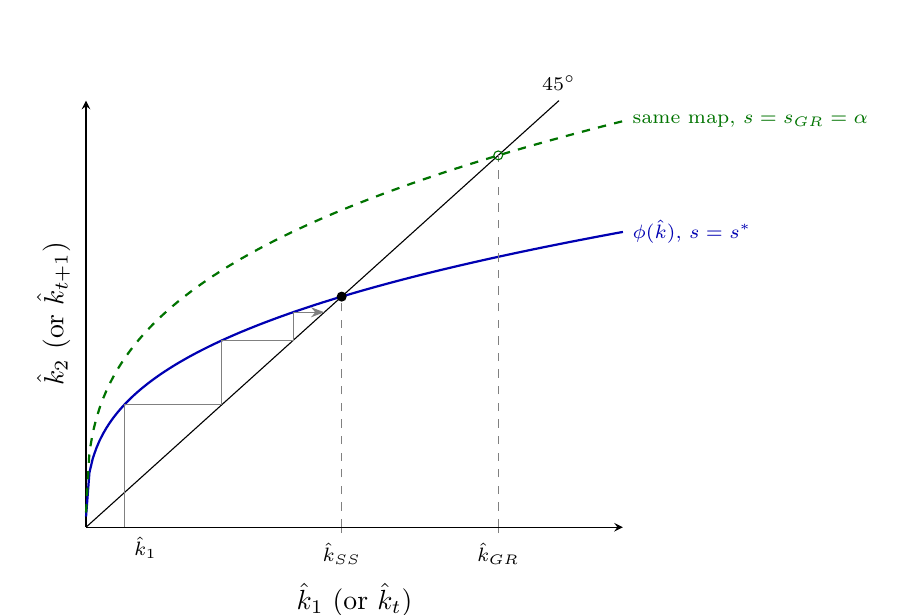
\begin{tikzpicture}
\begin{axis}[width=8.4cm,height=7cm,axis lines=left,xmin=0,xmax=2.1,ymin=0,ymax=1.85,clip=false,
  xlabel={$\hat k_1$ (or $\hat k_t$)},ylabel={$\hat k_2$ (or $\hat k_{t+1}$)},xtick={1,1.6124},
  xticklabels={$\hat k_{SS}$,$\hat k_{GR}$},ytick=\empty,every tick label/.append style={font=\scriptsize}]
\addplot[domain=0:1.85,thin,black]{x};
\addplot[domain=0.0001:2.1,samples=160,thick,blue!70!black]{x^(1/3)};
\addplot[domain=0.0001:2.1,samples=160,thick,dashed,green!45!black]{1.375*x^(1/3)};
\node[font=\scriptsize,anchor=south] at (axis cs:1.85,1.85){$45^\circ$};
\node[font=\scriptsize,blue!70!black,anchor=west] at (axis cs:2.1,1.281){$\phi(\hat k)$, $s=s^\ast$};
\node[font=\scriptsize,green!45!black,anchor=west] at (axis cs:2.1,1.761){same map, $s=s_{GR}=\alpha$};
\draw[gray,-{Stealth}](axis cs:0.15,0)--(axis cs:0.15,0.5313)--(axis cs:0.5313,0.5313)--(axis cs:0.5313,0.8099)
  --(axis cs:0.8099,0.8099)--(axis cs:0.8099,0.9321)--(axis cs:0.9321,0.9321);
\addplot[only marks,mark=*,mark size=1.6pt]coordinates{(1,1)};
\addplot[only marks,mark=o,mark size=1.6pt,green!45!black]coordinates{(1.6124,1.6124)};
\draw[dashed,gray](axis cs:1,0)--(axis cs:1,1);
\draw[dashed,gray](axis cs:1.6124,0)--(axis cs:1.6124,1.6124);
\node[font=\scriptsize,anchor=north west] at (axis cs:0.15,0){$\hat k_1$};
\end{axis}
\end{tikzpicture}\\
{\footnotesize Figure 3. The equilibrium law of motion (solid) crosses the 45-degree line once; the staircase
from a low $\hat k_1$ converges to $\hat k_{SS}$. Dashed: the same map with $s=\alpha$, whose fixed point is the
golden rule (used in 2.f). Drawn for $\alpha=1/3$, $\beta=0.96$, units chosen so that $\hat k_{SS}=1$.}
\end{center}
\intuicao{Patience and the productivity of capital set the saving rate; diminishing returns ($\alpha<1$) make
each extra unit of capital produce less, so saving a fixed share of a concave output cannot sustain unbounded
growth of $\hat k$.}
\refbib{Kurlat ch.~9, \S9.1 (firm FOCs, market clearing, $r=r^K-\delta$ with $\delta=1$); \S4.4, pp.~63--69
(factor shares, zero profit under constant returns); \S4.2, pp.~59--61 (stability).}
\rubrica{
\item Firm FOCs, $\Pi_1=\alpha Y_1$, $\Pi_2=0$, $1+r=\alpha Y_2/K_2$: 0.2 pt.
\item Market clearing $a_1=K_2$ (and goods): 0.1 pt. Saving rate $\alpha\beta/(1+\alpha\beta)$ derived: 0.2 pt.
\item Hours $L_1$, $L_2$: 0.1 pt. Map $\hat k_2(\hat k_1)$: 0.2 pt.
\item Diagram: axes, 45-degree line, concave map from the origin, $\hat k_{SS}$ at the crossing, stability argued: 0.2 pt.
\item Saving rate quoted from Solow's $s$ or left as a function of prices: 0 for that line. No market clearing ($K_2\neq a_1$): max.\ 0.5 pt. A map that does not cross the 45-degree line: 0 for the diagram.
}
\gap{Prova 01, 2.e: saving rate not derived; no market clearing $K_2=a_1$; diagram without a valid steady state.}
\end{sol}

\sub{2.f}{0.5 point} Discuss intuitively the relation between the model of items 2.c--2.e and the
Solow model of items 2.a--2.b. In particular, compare the saving rate found in 2.e with $s_{GR}$ and
explain the difference.
\resolespaco[5cm]
\begin{sol}
\begin{notacao}
\item As in 2.a--2.e. New: $\tilde k_t\equiv\hat k_t/L_1=K_t/(A_tL_1)>0$, capital per efficiency unit
of \emph{hours} (in 2.a, per efficiency unit of workers).
\end{notacao}
\passo{same law of motion}{Write \eqref{q2e:phi}, applied period after period, in terms of
$\tilde k_t=\hat k_t/L_1$:}
\begin{align}
L_1\tilde k_{t+1} &= \frac{s^\ast L_1^{1-\alpha}}{1+g}\,(L_1\tilde k_t)^{\alpha}\nonumber\\
&= \frac{s^\ast L_1}{1+g}\,\tilde k_t^{\alpha}\nonumber\\
(1+g)\tilde k_{t+1} &= s^\ast\tilde k_t^{\alpha}. \label{q2f:lom}
\end{align}
Set $\boxed{\delta=1}$ (capital used up in one period) and $\boxed{n=0}$ (one consumer) in the
Solow law of motion \eqref{q2a:lom}, which is equation \eqref{q2:K} divided as in 2.a:
\begin{align}
\tilde k_{t+1} &= \frac{(1-1)\tilde k_t+s\tilde k_t^{\alpha}}{(1+g)(1+0)}\nonumber\\
&= \frac{s\tilde k_t^{\alpha}}{1+g}\nonumber\\
(1+g)\tilde k_{t+1} &= s\,\tilde k_t^{\alpha}. \label{q2f:solow}
\end{align}
\eqref{q2f:lom} is \eqref{q2f:solow} with $s=s^\ast$. Indeed, by \eqref{q2e:kss},
\begin{align*}
\hat k_{SS} &= \left(\frac{s^\ast L_1^{1-\alpha}}{1+g}\right)^{\frac{1}{1-\alpha}}\\
&= L_1\left(\frac{s^\ast}{1+g}\right)^{\frac{1}{1-\alpha}}\\
&= L_1\left(\frac{s^\ast}{(1+g)(1+0)-(1-1)}\right)^{\frac{1}{1-\alpha}},
\end{align*}
which is 2.a's $\tilde k_{SS}$ \eqref{q2a:kss} times the hours worked.
\passo{what is new}{Solow \emph{assumes} $s$ and the labour input. Here both are \emph{chosen}:
$s^\ast=\alpha\beta/(1+\alpha\beta)$ in \eqref{q2e:s} comes from patience $\beta$ and the return to
capital $\alpha$, and log utility makes it constant (independent of $K$, $A$, $g$) --- a
microfoundation for Solow's constant saving rate. Hours $L_1$ in \eqref{q2e:L1} depend on the taste
for leisure $\gamma$ and on $\beta$.}
\passo{against the golden rule}{Compare \eqref{q2e:s} with $s_{GR}=\alpha$ from \eqref{q2b:sgr}:}
\begin{align*}
s^\ast<\alpha &\iff \frac{\alpha\beta}{1+\alpha\beta}<\alpha\\
&\iff \frac{\beta}{1+\alpha\beta}<1\\
&\iff \beta<1+\alpha\beta\\
&\iff \beta(1-\alpha)<1,
\end{align*}
always true, since $\beta<1$ and $1-\alpha<1$. So $\boxed{s^\ast<\alpha}$ and $\hat k_{SS}<\hat k_{GR}$
(Figure 3): the competitive economy accumulates \emph{less} than the golden rule. Even as
$\beta\to1$, $s^\ast\to\alpha/(1+\alpha)<\alpha$: here saving finances one period of consumption
only, since the horizon ends.
\passo{why this is not a failure}{The golden rule maximises steady-state consumption and ignores that
consumption earlier is worth more to an impatient consumer ($\beta<1$) and that reaching more capital costs
consumption on the way. Markets here are complete and competitive, with no externalities: by the first welfare
theorem the equilibrium is Pareto efficient, and it is below the golden rule, i.e.\ dynamically efficient. The
golden rule is a property of steady states, not a welfare criterion.}
\refbib{Kurlat \S4.3, pp.~61--63; ch.~9, \S9.2 (first welfare theorem) and \S9.3 (comparison with the golden rule).}
\rubrica{
\item Same law of motion with $\delta=1$, $n=0$: 0.1 pt.
\item Saving (and hours) chosen, not assumed, and from which primitives: 0.2 pt.
\item $s^\ast<\alpha$ shown, with the reason (impatience; golden rule not a welfare criterion): 0.2 pt.
\item ``It is Solow with $\delta=1$ and $n=0$'' and nothing else: max.\ 0.1 pt.
}
\gap{Prova 01, 2.f: the endogenous saving rate and its comparison with $s_{GR}$ were missing.}
\end{sol}

% =============================================================================
\questao{3}{3}{Consider the simplified New Keynesian model of Benigno (2015), based on the aggregate
demand and supply equations below (barred variables are long-run values, when all firms reset their
prices; the others are short-run values):
\begin{align}
y &= \bar y+(g-\bar g)-\sigma\left[i-(\bar p-p)\right]-\sigma\ln\beta, \tag{AD}\label{q3:AD}\\
p-p^e &= \kappa\,(y-y_n), \tag{AS}\label{q3:AS}
\end{align}
where $p^e$ is the price set by the firms that cannot reset prices and $y_n$ is short-run natural output,
\begin{equation}
y_n=\frac{1+\eta}{\sigma^{-1}+\eta}\,a+\frac{\sigma^{-1}}{\sigma^{-1}+\eta}\,g-\frac{1}{\sigma^{-1}+\eta}\,\mu , \tag{YN}\label{q3:YN}
\end{equation}
$\mu$ being the mark-up; $\bar y$ is given by the same expression evaluated at the long-run values
$\bar a$, $\bar g$, $\bar\mu$; and $y_e=\frac{1+\eta}{\sigma^{-1}+\eta}a+\frac{\sigma^{-1}}{\sigma^{-1}+\eta}g$ is the
efficient level of output. All variables are log deviations from an efficient steady state. Initially
$a=\bar a=g=\bar g=\mu=\bar\mu=0$, $\bar p=p^e$, and the central bank sets $i=\rho\equiv-\ln\beta$, so that
$y=y_n=y_e=\bar y$ and $p=p^e$.}

\sub{3.a}{1 point} News arrives that productivity will be permanently higher in the long run: $\bar a$
rises by $d\bar a>0$, while current productivity $a$ does not change. With $i$ unchanged, represent
graphically, explaining economically why, the initial equilibrium and the shift that defines the new
equilibrium. Compute $dy$ and $dp$. Indicate the gap $y-y_n$ and the gap $y-y_e$ and use both in your
explanation. Is this boom good for welfare today? Justify.
\resolespaco[7cm]
\begin{sol}
\begin{notacao}
\item $y$, $p$: output and price level today; $\bar y$, $\bar p$: their long-run values, when all
firms have reset prices. All are log deviations from the efficient steady state.
\item $p^e$: the price preset by the firms that cannot reset this period.
\item $i$: nominal interest rate, the central bank's instrument. $\beta\in(0,1)$: discount factor;
$\rho\equiv-\ln\beta>0$: the initial (neutral) rate.
\item $a$, $\bar a$: productivity today and in the long run. $g$, $\bar g$: government spending.
$\mu$, $\bar\mu$: the firms' mark-up. All start at 0.
\item $\sigma>0$: intertemporal elasticity of substitution. $\eta>0$: inverse Frisch elasticity of
labour supply. $\kappa>0$: slope of AS.
\item $y_n$: natural output (flexible prices, with the mark-up). $y_e$: efficient output (no mark-up).
\item $\Gamma\equiv\frac{1+\eta}{\sigma^{-1}+\eta}>0$: response of $y_n$, $y_e$ and $\bar y$ to
productivity.
\end{notacao}
\passo{0, the remaining statement equations}{With $\Gamma$ as defined above, the statement gives
long-run output (the expression \eqref{q3:YN} at long-run values) and efficient output:}
\begin{align}
\bar y &= \Gamma\,\bar a+\frac{\sigma^{-1}}{\sigma^{-1}+\eta}\,\bar g-\frac{1}{\sigma^{-1}+\eta}\,\bar\mu, \label{q3:ybar}\\
y_e &= \Gamma\,a+\frac{\sigma^{-1}}{\sigma^{-1}+\eta}\,g. \label{q3:ye}
\end{align}
Substitute $\rho=-\ln\beta$ into \eqref{q3:AD}, then use the initial values $g=\bar g=0$ and
$\bar p=p^e$:
\begin{align}
y &= \bar y+(g-\bar g)-\sigma\left[i-(\bar p-p)\right]-\sigma(-\rho)\nonumber\\
&= \bar y+(g-\bar g)-\sigma(i-\rho)-\sigma(p-\bar p)\nonumber\\
&= \bar y+(0-0)-\sigma(i-\rho)-\sigma\big(p-(p^e)\big)\nonumber\\
&= \bar y-\sigma(i-\rho)-\sigma(p-p^e). \label{q3:ADr}
\end{align}
\passo{which bar moves which curve}{Differentiate \eqref{q3:ybar} with only $\bar a$ moving:}
\begin{equation}
d\bar y=\Gamma\,d\bar a>0. \label{q3a:dybar}
\end{equation}
$\bar y$ is in AD \eqref{q3:ADr}, so \boxed{\text{AD shifts right}} by $\Gamma d\bar a$ at every
$p$ (up by $\Gamma d\bar a/\sigma$). $y_n$ in \eqref{q3:YN} and $y_e$ in \eqref{q3:ye} depend on the
\emph{current} $a$, $g$, $\mu$, none of which moved: \boxed{\text{AS does not move}} (it still passes
through $(y_n,p^e)$), and $y_e=y_n=0$ still.
\passo{why AD moves (Euler)}{Long-run consumption $\bar c=\bar y$ rises: households expect higher permanent
income and, to smooth consumption, want to consume more \emph{today} at the same real rate
$i-(\bar p-p)$. Current demand for goods rises at every price level.}
\passo{new equilibrium}{With $i=\rho$, \eqref{q3:ADr} and \eqref{q3a:dybar} give AD; with $y_n=0$,
\eqref{q3:AS} gives AS:}
\begin{align}
y &= (\Gamma\,d\bar a)-\sigma(\rho-\rho)-\sigma(p-p^e)\nonumber\\
&= \Gamma\,d\bar a-\sigma(p-p^e), \label{q3a:AD}\\
p-p^e &= \kappa\,(y-0)\nonumber\\
&= \kappa\,y. \label{q3a:AS}
\end{align}
Substitute \eqref{q3a:AS} into \eqref{q3a:AD}:
\begin{align*}
y &= \Gamma\,d\bar a-\sigma(\kappa\,y)\\
y(1+\sigma\kappa) &= \Gamma\,d\bar a.
\end{align*}
Divide by $1+\sigma\kappa$ (the initial $y$ is 0, so $y=dy$):
\begin{equation}
\boxed{dy=\frac{\Gamma\,d\bar a}{1+\sigma\kappa}>0} \label{q3a:dy}
\end{equation}
Substitute \eqref{q3a:dy} into \eqref{q3a:AS}:
\begin{align}
dp &= \kappa\,dy\nonumber\\
&= \kappa\left(\frac{\Gamma\,d\bar a}{1+\sigma\kappa}\right)\nonumber\\
&= \boxed{\frac{\kappa\,\Gamma\,d\bar a}{1+\sigma\kappa}>0}. \label{q3a:dp}
\end{align}
\passo{the two gaps}{Since $y_n=y_e=0$, both gaps equal \eqref{q3a:dy}. $y-y_n=dy>0$: output above
natural, which is why prices rise in \eqref{q3a:dp} (AS: flexible-price firms face higher real
marginal cost, because households must be paid a higher real wage to work more). $y-y_e=dy>0$:
output above the efficient level as well.
Chain: $\bar a\uparrow\to\bar y\uparrow\to c\uparrow$ (Euler) $\to$ AD right $\to y>y_n\to$ marginal cost $\uparrow\to$
flexible firms raise $p$ $\to$ real rate $i-(\bar p-p)\uparrow$, which limits the rise in $y$ (movement along AD).
Firms with preset prices keep $p^e$ and produce whatever is demanded.}
\passo{welfare}{\textbf{No.} Today's technology is unchanged, so the efficient output today is unchanged.
The extra output is produced by working beyond the point where the MRS between leisure and consumption equals
today's productivity, and the price surprise $p>p^e$ creates price dispersion across identical firms. Both
terms of the welfare loss are positive: the economy is overheating on a forecast.}
\begin{center}
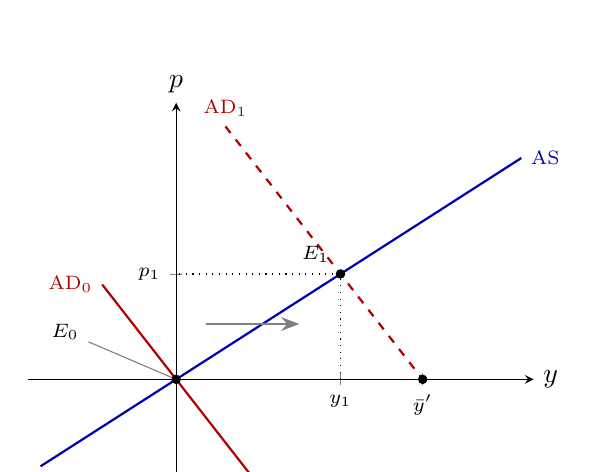
\begin{tikzpicture}
\begin{axis}[width=8cm,height=6.4cm,axis lines=middle,xmin=-0.6,xmax=1.45,ymin=-0.65,ymax=1.75,clip=false,
  xlabel={$y$},ylabel={$p$},xtick={0.6667,1},xticklabels={$y_1$,$\bar y'$},ytick={0.6667},yticklabels={$p_1$},
  every tick label/.append style={font=\scriptsize},x label style={anchor=west},y label style={anchor=south}]
\addplot[thick,blue!70!black,domain=-0.55:1.4]{x};
\addplot[thick,red!70!black,domain=-0.3:0.3]{-2*x};
\addplot[thick,red!70!black,dashed,domain=0.2:1.0]{2-2*x};
\node[font=\scriptsize,blue!70!black,anchor=west] at (axis cs:1.4,1.4){AS};
\node[font=\scriptsize,red!70!black,anchor=east] at (axis cs:-0.3,0.6){AD$_0$};
\node[font=\scriptsize,red!70!black,anchor=south] at (axis cs:0.2,1.6){AD$_1$};
\addplot[only marks,mark=*,mark size=1.5pt]coordinates{(0,0)(0.6667,0.6667)(1,0)};
\node[font=\scriptsize] (e0) at (axis cs:-0.45,0.3){$E_0$};
\draw[gray,thin](e0)--(axis cs:0,0);
\node[font=\scriptsize,anchor=south east] at (axis cs:0.66,0.68){$E_1$};
\draw[dotted](axis cs:0.6667,0)--(axis cs:0.6667,0.6667)--(axis cs:0,0.6667);
\draw[-{Stealth},thick,gray](axis cs:0.12,0.35)--(axis cs:0.5,0.35);
\end{axis}
\end{tikzpicture}\\
{\footnotesize Figure 4. News of higher $\bar a$ shifts AD right (it now passes through $(\bar y',\bar p)$ at $i=\rho$);
AS stays. $E_1$: $y_1-y_n=y_1-y_e>0$ and $p_1>p^e$. (Drawn for $\sigma=0.5$, $\kappa=1$, $\Gamma d\bar a=1$; the origin is
$(y_n,p^e)$.)}
\end{center}
\intuicao{Expectations about the future move demand today. Supply today has not changed, so the extra demand
can only be met by working harder with the same technology, and prices rise.}
\refbib{Benigno (2015) \S6.3, Fig.~8, pp.~511--513; \S5, eqs.~(20)--(21), pp.~509--511; \S4.2--\S4.4 ($y_n$, $y_e$), pp.~508--509.}
\rubrica{
\item AD shifts right, with the Euler/permanent-income reason: 0.3 pt.
\item AS does not move, because $y_n$ depends on current $a,\mu$ only: 0.2 pt.
\item $dy$ and $dp$: 0.2 pt.
\item Both gaps signed and used in the explanation: 0.2 pt. Welfare verdict with the reason: 0.1 pt.
\item Graph lines are inside the first two items (axes $y,p$; AD$_0$, AD$_1$, AS named; $E_0$, $E_1$; direction of the shift).
\item Shifting AS (treating the news as current productivity): max.\ 0.3 pt. Signs of $dy$, $dp$ inconsistent with the graph: $-0.2$.
}
\end{sol}

\sub{3.b}{1 point} Based on the previous item, explain intuitively what a monetary authority committed
to price stability should do after the news, by how much it must move its instrument, and what is the
economic cost of doing so. Show graphically the paths of $y$ and $p$ in the short and in the long run,
with and without that response. A commentator claims that ``whatever the central bank does, it must
give up either price stability or a closed output gap''. Evaluate the claim.
\resolespaco[7cm]
\begin{sol}
\begin{notacao}
\item As in 3.a. New: $r_n$, the natural real interest rate, the real rate that clears today's goods
market at natural output.
\end{notacao}
\passo{target}{Price stability: $p=p^e$. On AS \eqref{q3:AS} this requires $y=y_n$, and since
$y_n=y_e$ here, it also gives $y=y_e$.}
\passo{instrument}{AD must pass through $(y_n,p^e)=(0,p^e)$. Set $y=0$ and $p=p^e$ in \eqref{q3:ADr},
with $\bar y=\Gamma d\bar a$ from \eqref{q3a:dybar}:}
\begin{align*}
0 &= (\Gamma\,d\bar a)-\sigma(i-\rho)-\sigma(p^e-p^e)\\
0 &= \Gamma\,d\bar a-\sigma(i-\rho)\\
\sigma(i-\rho) &= \Gamma\,d\bar a.
\end{align*}
Divide by $\sigma$:
\begin{equation}
\boxed{i=\rho+\frac{\Gamma\,d\bar a}{\sigma}} \label{q3b:i}
\end{equation}
\textbf{Raise} $i$ by $\Gamma d\bar a/\sigma>0$. The natural real rate is
\begin{equation}
r_n=\rho+\sigma^{-1}(\bar y-y_n). \label{q3b:rn}
\end{equation}
Differentiate \eqref{q3b:rn} and substitute \eqref{q3a:dybar} and $dy_n=0$:
\begin{align*}
dr_n &= \sigma^{-1}\big[(\Gamma\,d\bar a)-(0)\big]\\
&= \frac{\Gamma\,d\bar a}{\sigma}.
\end{align*}
The rise in \eqref{q3b:i} is exactly the rise in $r_n$. The future is richer, so the real rate that clears today's goods market
at natural output is higher. AD returns to AD$_0$ in Figure 4.
\passo{cost}{\textbf{None} in terms of the two objectives: after the rise $y=y_n=y_e$ and $p=p^e$. The shock is
\emph{efficient}: it does not separate $y_n$ from $y_e$ (no mark-up moved), so one instrument closes both gaps
(divine coincidence). The commentator is wrong for this shock. A cut, the instinct to ``support the good
news'', would push output and prices further up.}
\passo{long run}{In period 2 all prices adjust and $y=\bar y'=\Gamma d\bar a$, $p=\bar p$, with or without the
response. The higher rate does not cancel the gain; it \emph{times} it: households wait for the productivity to
arrive instead of working beyond the efficient level today. The same response is right if the news is only
optimism; the model cannot tell the two apart in the short run.}
\begin{center}
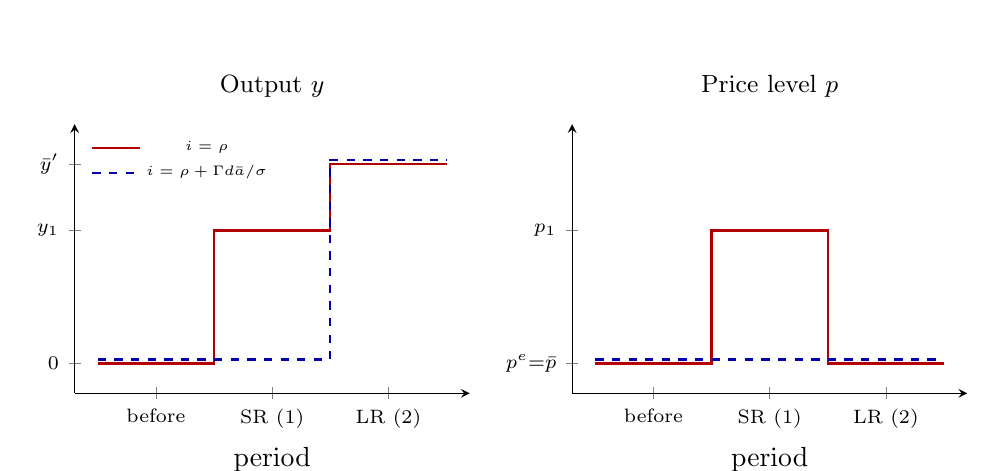
\begin{tikzpicture}
\begin{axis}[name=py,width=6.6cm,height=5cm,axis lines=left,xmin=-0.2,xmax=3.2,ymin=-0.15,ymax=1.2,
  xlabel={period},xtick={0.5,1.5,2.5},xticklabels={before,SR (1),LR (2)},ytick={0,0.6667,1},
  yticklabels={$0$,$y_1$,$\bar y'$},title={\small Output $y$},every tick label/.append style={font=\scriptsize},
  legend style={font=\tiny,draw=none,at={(0.02,0.98)},anchor=north west}]
\addplot[thick,red!70!black,const plot] coordinates {(0,0)(1,0.6667)(2,1)(3,1)};
\addplot[thick,blue!70!black,dashed,const plot] coordinates {(0,0.02)(1,0.02)(2,1.02)(3,1.02)};
\legend{$i=\rho$,$i=\rho+\Gamma d\bar a/\sigma$}
\end{axis}
\begin{axis}[at={(py.east)},anchor=west,xshift=1.3cm,width=6.6cm,height=5cm,axis lines=left,xmin=-0.2,xmax=3.2,
  ymin=-0.15,ymax=1.2,xlabel={period},xtick={0.5,1.5,2.5},xticklabels={before,SR (1),LR (2)},ytick={0,0.6667},
  yticklabels={$p^e{=}\bar p$,$p_1$},title={\small Price level $p$},every tick label/.append style={font=\scriptsize}]
\addplot[thick,red!70!black,const plot] coordinates {(0,0)(1,0.6667)(2,0)(3,0)};
\addplot[thick,blue!70!black,dashed,const plot] coordinates {(0,0.02)(3,0.02)};
\end{axis}
\end{tikzpicture}\\
{\footnotesize Figure 5. Solid: no response, a boom with a price surprise in the short run. Dashed: the rate rise
keeps $y=y_n=y_e$ and $p=p^e$ in the short run; in the long run both paths reach $\bar y'$ and $\bar p$.}
\end{center}
\intuicao{The central bank's job is to set the real rate to the one the economy would have with flexible prices.
Good news about the future raises that rate; tracking it is not ``fighting'' the news.}
\refbib{Benigno (2015) \S6.3, Fig.~8, pp.~511--513 (optimal response to expected productivity); \S5 ($r_n$); \S11, p.~522
(no trade-off when $y_n=y_e$).}
\rubrica{
\item Raise $i$, with the mechanism (AD back through $(y_n,p^e)$): 0.3 pt.
\item Size $\Gamma d\bar a/\sigma$, read as the rise in $r_n$: 0.2 pt.
\item Cost: none, both gaps closed, because the shock is efficient ($y_n=y_e$); claim rejected: 0.3 pt.
\item Paths SR/LR with and without the response: 0.2 pt (0.1 if the long run is missing).
\item Cutting $i$: max.\ 0.2 pt on the item. ``Cost: a recession'' (a trade-off asserted): max.\ 0.5 pt.
}
\gap{Prova 01, 3.a--3.b: which bar moves which curve; sign of the policy response to a pure AD shift; the cost
of a response when there is no trade-off.}
\end{sol}

\sub{3.c}{1 point} Suppose the monetary authority represents society's preferences by the quadratic
loss function, with parameter $\phi\geq0$,
\begin{equation}
L=\frac12\left(y-y_e\right)^2+\frac{\phi}{2\kappa}\left(p-p^e\right)^2 . \tag{LF}\label{q3:LF}
\end{equation}
In the same period as the news of item 3.a, the government temporarily raises a tax on firms' sales
revenue (an IPI-like tax), which raises the current mark-up by $d\mu>0$; the long-run mark-up $\bar\mu$
does not change. Derive the optimal monetary-policy rule (IT), find the optimal $y$, $p$ and $i$, and
show graphically the optimal policy. Discuss how your answer depends on $\phi$, separating the part of
the optimal response that answers the news from the part that answers the mark-up shock.
\resolespaco[8cm]
\begin{sol}
\begin{notacao}
\item As in 3.a--3.b. New: $\phi\ge0$, the weight on price surprises in \eqref{q3:LF}.
\item $m\equiv\frac{d\mu}{\sigma^{-1}+\eta}>0$: the fall in natural output caused by the tax.
$y_n'$: natural output after the tax.
\item $y^\ast$, $p^\ast$, $i^\ast$: optimal output, price level and interest rate; $O=(y^\ast,p^\ast)$.
\item $N$, $y_N$: the point on the new AS, and its output, reached when $i$ only offsets the news.
\end{notacao}
\passo{what the tax moves}{Differentiate \eqref{q3:YN} with respect to the current mark-up:}
\begin{equation}
y_n'=-\frac{d\mu}{\sigma^{-1}+\eta}=-m<0. \label{q3c:yn}
\end{equation}
Current natural output falls, so \textbf{AS shifts up/left} through $(y_n',p^e)$. $y_e$ in
\eqref{q3:ye} has no $\mu$: $y_e=0$ is unchanged. Now $y_n\neq y_e$: the tax is an
\emph{inefficient} shock. $\bar\mu$ is unchanged, so by \eqref{q3:ybar} the AD shift is only the
news ($\bar y=\Gamma d\bar a$, \eqref{q3a:dybar}).
\passo{AS is the constraint}{The central bank moves AD with $i$; for any point on AS there is an
$i$ that puts AD through it. AS, with $p^e$ preset, is what policy cannot move within the period:
it is the feasible set. So choose $y$ on AS and recover $i$ from AD. By \eqref{q3:AS} with
\eqref{q3c:yn}, the constraint is}
\begin{equation}
p-p^e=\kappa\,(y-y_n'). \label{q3c:AS}
\end{equation}
Substitute \eqref{q3c:AS} into \eqref{q3:LF}:
\begin{align}
L(y) &= \tfrac12(y-y_e)^2+\tfrac{\phi}{2\kappa}\big[\kappa\,(y-y_n')\big]^2\nonumber\\
&= \tfrac12(y-y_e)^2+\tfrac{\phi}{2\kappa}\kappa^2(y-y_n')^2\nonumber\\
&= \tfrac12(y-y_e)^2+\tfrac{\phi\kappa}{2}(y-y_n')^2 . \label{q3c:L}
\end{align}
\passo{targeting rule}{Differentiate \eqref{q3c:L} and set it to zero:}
\begin{equation}
\frac{dL}{dy}=(y-y_e)+\phi\kappa\,(y-y_n')=0. \label{q3c:foc}
\end{equation}
By \eqref{q3c:AS}, $\kappa(y-y_n')=p-p^e$. Substitute this into \eqref{q3c:foc}:
\begin{equation}
\boxed{(y-y_e)+\phi\,(p-p^e)=0}\qquad\text{(IT: a line through $(y_e,p^e)$ with slope $-1/\phi$).} \label{q3c:IT}
\end{equation}
SOC: from \eqref{q3c:L}, $d^2L/dy^2=1+\phi\kappa>0$.
\passo{optimal point}{Solve \eqref{q3c:foc} for $y$:}
\begin{align}
y(1+\phi\kappa) &= y_e+\phi\kappa\,y_n'\nonumber\\
y^\ast &= \frac{y_e+\phi\kappa\,y_n'}{1+\phi\kappa}. \label{q3c:ystar}
\end{align}
Substitute $y_e=0$ and \eqref{q3c:yn} into \eqref{q3c:ystar}:
\begin{align}
y^\ast &= \frac{(0)+\phi\kappa\,(-m)}{1+\phi\kappa}\nonumber\\
&= \boxed{-\frac{\phi\kappa}{1+\phi\kappa}\,m<0} \label{q3c:ystarm}
\end{align}
Substitute \eqref{q3c:ystarm} and \eqref{q3c:yn} into \eqref{q3c:AS}:
\begin{align}
p^\ast-p^e &= \kappa(y^\ast-y_n')\nonumber\\
&= \kappa\left[\left(-\frac{\phi\kappa}{1+\phi\kappa}\,m\right)-(-m)\right]\nonumber\\
&= \kappa\left(m-\frac{\phi\kappa\,m}{1+\phi\kappa}\right)\nonumber\\
&= \boxed{\frac{\kappa}{1+\phi\kappa}\,m>0}. \label{q3c:pstar}
\end{align}
Check in \eqref{q3c:IT}:
\begin{align*}
(y^\ast-y_e)+\phi(p^\ast-p^e) &= \left[\left(-\frac{\phi\kappa}{1+\phi\kappa}\,m\right)-(0)\right]
+\phi\left(\frac{\kappa}{1+\phi\kappa}\,m\right)\\
&= \frac{-\phi\kappa m+\phi\kappa m}{1+\phi\kappa}=0\ \checkmark
\end{align*}
The bank splits the shock: output below efficient \emph{and} prices above $p^e$.
\passo{optimal rate}{Evaluate AD \eqref{q3:ADr} at $(y^\ast,p^\ast)$, with $\bar y=\Gamma d\bar a$,
and solve for $i^\ast$:}
\begin{align}
(y^\ast) &= (\Gamma\,d\bar a)-\sigma(i^\ast-\rho)-\sigma\big((p^\ast)-p^e\big)\nonumber\\
\sigma(i^\ast-\rho) &= \Gamma\,d\bar a-y^\ast-\sigma(p^\ast-p^e)\nonumber\\
i^\ast &= \rho+\frac{\Gamma\,d\bar a-y^\ast}{\sigma}-(p^\ast-p^e). \label{q3c:igen}
\end{align}
Substitute \eqref{q3c:ystarm} and \eqref{q3c:pstar} into \eqref{q3c:igen}:
\begin{align}
i^\ast &= \rho+\frac{\Gamma\,d\bar a-\left(-\frac{\phi\kappa}{1+\phi\kappa}\,m\right)}{\sigma}
-\left(\frac{\kappa}{1+\phi\kappa}\,m\right)\nonumber\\
&= \rho+\frac{\Gamma\,d\bar a}{\sigma}+\frac{\phi\kappa m}{\sigma(1+\phi\kappa)}-\frac{\kappa m}{1+\phi\kappa}. \label{q3c:i4}
\end{align}
Put the last two terms of \eqref{q3c:i4} over the common denominator $\sigma(1+\phi\kappa)$:
\begin{equation}
\boxed{i^\ast=\rho+\underbrace{\frac{\Gamma\,d\bar a}{\sigma}}_{\text{news}}
+\underbrace{\frac{\kappa\,m\,(\phi-\sigma)}{\sigma(1+\phi\kappa)}}_{\text{mark-up}}} \label{q3c:istar}
\end{equation}
\passo{the news part does not depend on $\phi$}{The news moves neither $y_n$ nor $y_e$, so by
\eqref{q3c:ystar} it does not move the optimal point $O=(y^\ast,p^\ast)$ on AS. The bank simply
undoes the AD shift, $di=\Gamma d\bar a/\sigma$ in \eqref{q3c:istar}, for \emph{any} $\phi$, exactly
as in \eqref{q3b:i}.}
\passo{the mark-up part depends on $\phi$ against $\sigma$}{Substitute the news-offset rate
\eqref{q3b:i} and $\bar y=\Gamma d\bar a$ into AD \eqref{q3:ADr}: AD is back at AD$_0$. Then
substitute \eqref{q3c:AS} for $p-p^e$ to find the point $N$:}
\begin{align}
y &= (\Gamma\,d\bar a)-\sigma\left(\frac{\Gamma\,d\bar a}{\sigma}\right)-\sigma(p-p^e)\nonumber\\
&= -\sigma(p-p^e)\nonumber\\
y &= -\sigma\big[\kappa\,(y-y_n')\big]\nonumber\\
y_N &= \frac{\sigma\kappa}{1+\sigma\kappa}\,y_n'. \label{q3c:yN}
\end{align}
Subtract \eqref{q3c:yN}, with $y_n'=-m$, from \eqref{q3c:ystarm}:
\begin{align}
y^\ast-y_N &= \left(-\frac{\phi\kappa}{1+\phi\kappa}\,m\right)-\frac{\sigma\kappa}{1+\sigma\kappa}\,(-m)\nonumber\\
&= -\frac{\phi\kappa m}{1+\phi\kappa}+\frac{\sigma\kappa m}{1+\sigma\kappa}\nonumber\\
&= \frac{\kappa m(\sigma-\phi)}{(1+\phi\kappa)(1+\sigma\kappa)}. \label{q3c:diff}
\end{align}
If $\phi>\sigma$ (the IT line is flatter than AD), \eqref{q3c:diff} is negative: the bank raises $i$
further and accepts a deeper output loss for less price movement; if $\phi<\sigma$ it raises $i$ by
less than the news alone requires. Limits of \eqref{q3c:ystarm}, \eqref{q3c:pstar} and
\eqref{q3c:istar}:
\begin{align*}
\phi\to\infty\ \text{(strict price stability)}:&\quad y^\ast=y_n',\quad p^\ast=p^e,\quad
i^\ast=\rho+\frac{\Gamma d\bar a+m}{\sigma},\\
\phi=0:&\quad y^\ast=y_e,\quad p^\ast=p^e+\kappa m,\quad i^\ast=\rho+\frac{\Gamma d\bar a}{\sigma}-\kappa m.
\end{align*}
\passo{trade-off}{Unlike 3.b there is a trade-off: $y_n'\neq y_e$, so no rate closes both gaps;
$\phi$ chooses where on AS to sit.}
\begin{center}\begin{minipage}{\linewidth}\centering
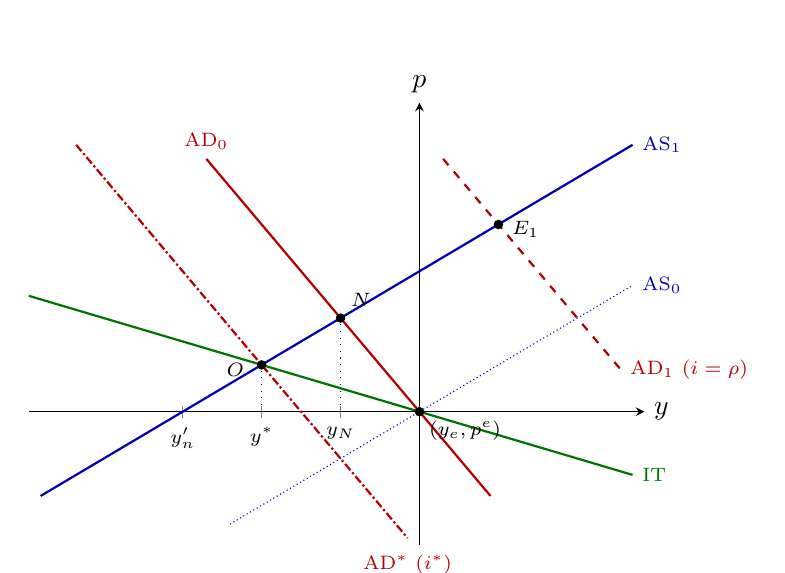
\begin{tikzpicture}
\begin{axis}[width=9.4cm,height=7.2cm,axis lines=middle,xmin=-1.65,xmax=0.95,ymin=-0.95,ymax=2.2,clip=false,
  xlabel={$y$},ylabel={$p$},xtick={-1,-0.6667,-0.3333},xticklabels={$y_n'$,$y^\ast$,$y_N$},ytick=\empty,
  every tick label/.append style={font=\scriptsize},x label style={anchor=west},y label style={anchor=south}]
\addplot[densely dotted,blue!70!black,domain=-0.8:0.9]{x};
\addplot[thick,blue!70!black,domain=-1.6:0.9]{x+1};
\addplot[thick,green!45!black,domain=-1.65:0.9]{-x/2};
\addplot[thick,red!70!black,dashed,domain=0.1:0.85]{2-2*x};
\addplot[thick,red!70!black,domain=-0.9:0.3]{-2*x};
\addplot[thick,red!70!black,densely dashdotted,domain=-1.45:-0.05]{-1-2*x};
\node[font=\scriptsize,blue!70!black,anchor=west] at (axis cs:0.9,0.9){AS$_0$};
\node[font=\scriptsize,blue!70!black,anchor=west] at (axis cs:0.9,1.9){AS$_1$};
\node[font=\scriptsize,green!45!black,anchor=west] at (axis cs:0.9,-0.45){IT};
\node[font=\scriptsize,red!70!black,anchor=west] at (axis cs:0.85,0.3){AD$_1$ ($i=\rho$)};
\node[font=\scriptsize,red!70!black,anchor=south] at (axis cs:-0.9,1.8){AD$_0$};
\node[font=\scriptsize,red!70!black,anchor=north] at (axis cs:-0.05,-0.95){AD$^\ast$ ($i^\ast$)};
\addplot[only marks,mark=*,mark size=1.5pt]coordinates{(0.3333,1.3333)(-0.3333,0.6667)(-0.6667,0.3333)(0,0)};
\node[font=\scriptsize,anchor=west] at (axis cs:0.35,1.3){$E_1$};
\node[font=\scriptsize,anchor=south west] at (axis cs:-0.33,0.68){$N$};
\node[font=\scriptsize,anchor=east] at (axis cs:-0.7,0.3){$O$};
\node[font=\scriptsize,anchor=north west] at (axis cs:0,0){$(y_e,p^e)$};
\draw[dotted](axis cs:-0.6667,0)--(axis cs:-0.6667,0.3333);
\draw[dotted](axis cs:-0.3333,0)--(axis cs:-0.3333,0.6667);
\end{axis}
\end{tikzpicture}\\
{\footnotesize Figure 6. The tax shifts AS from AS$_0$ to AS$_1$ (through $(y_n',p^e)$); the news shifts AD from AD$_0$ to
AD$_1$. With $i=\rho$ the economy is at $E_1$. Offsetting the news alone brings AD back to AD$_0$ and the economy to
$N$. The optimum $O$ is where AS$_1$ meets the IT line; drawn for $\phi=2>\sigma=0.5$, so the bank raises $i$ beyond
the news offset, to AD$^\ast$. ($\kappa=1$, $\Gamma d\bar a=m=1$.)}
\end{minipage}\end{center}
\intuicao{Two shocks, two different jobs. The news is a demand shock with no trade-off: offset it fully. The tax is a
cost shock that drives a wedge between natural and efficient output: no rate fixes both gaps, so the convex loss
spreads the miss, and $\phi$ says how much of it goes into prices.}
\refbib{Benigno (2015) \S11, eqs.~(33)--(35), Fig.~14, pp.~521--523; \S7, Fig.~9, pp.~513--514 (mark-up shocks; taxes in
$1+\mu$); \S4.4, p.~509.}
\rubrica{
\item AS shifts up/left, $y_e$ does not move, AD shift from the news only: 0.15 pt.
\item Why AS is the constraint; substitution into $L$: 0.15 pt.
\item Targeting rule $(y-y_e)+\phi(p-p^e)=0$ from $dL/dy=0$: 0.2 pt.
\item $y^\ast$, $p^\ast$: 0.15 pt. $i^\ast$ with its two components: 0.15 pt.
\item Role of $\phi$: news part independent of $\phi$; mark-up part signed by $\phi-\sigma$; a limit case: 0.1 pt.
\item Graph (AS$_1$, IT, AD before/after, $O$ labelled): 0.1 pt.
\item Differentiating in $i$ with AD as the constraint, or targeting $y_n$ instead of $y_e$: max.\ 0.4 pt. Claiming the whole
response (news included) depends on $\phi$ versus $\sigma$: max.\ 0.6 pt.
}
\gap{Prova 01, 3.c: $dL/dy=0$ along AS not used; the response to news wrongly made to depend on $\phi$.}
\end{sol}

\ifsolucoes\else
\vfill
\begin{center}\footnotesize\textit{End of exam.}\end{center}
\fi

\end{document}
